\documentclass[11pt,a4paper]{article}
\usepackage[margin=2.2cm]{geometry}
\usepackage{amsmath,amssymb,mathtools}
\usepackage{graphicx}
\usepackage{booktabs}
\usepackage{longtable}
\usepackage{array}
\usepackage{hyperref}
\usepackage{placeins}
\usepackage{xcolor}
\usepackage{caption}
\usepackage{subcaption}
\usepackage{enumitem}
\usepackage{algorithm}
\usepackage{algpseudocode}
\usepackage{listings}
\usepackage{siunitx}
\usepackage{microtype}
\usepackage{multirow}
\hypersetup{colorlinks=true,linkcolor=blue,urlcolor=blue,citecolor=blue}

\lstdefinestyle{cfg}{
  basicstyle=\ttfamily\footnotesize,
  breaklines=true,
  columns=fullflexible,
  frame=single,
  rulecolor=\color{black!30},
  showstringspaces=false,
}
\lstset{style=cfg}

\algrenewcommand\algorithmicrequire{\textbf{Input:}}
\algrenewcommand\algorithmicensure{\textbf{Output:}}

\newcommand{\code}[1]{\texttt{\small #1}}
\newcommand{\Vm}{V_{\text{m}}}
\newcommand{\Iion}{I_{\mathrm{ion}}}
\newcommand{\Dten}{\mathbf{D}}
\newcommand{\grad}{\nabla}
\newcommand{\divg}{\nabla\!\cdot}
\newcommand{\Mmass}{\mathbf{M}}
\newcommand{\Kstif}{\mathbf{K}}
\newcommand{\Lop}{\mathbf{L}}
\newcommand{\Aimp}{\mathbf{A}}
\newcommand{\Bimp}{\mathbf{B}}
\newcommand{\Fres}{\mathsf{F}}
\newcommand{\R}{\mathbb{R}}
\newcommand{\norm}[1]{\left\lVert #1 \right\rVert}
\title{Solver Specification and Verification Report:\\
       \texorpdfstring{\code{highOrderManufacturedFDAImplicitPETScDistributed}}{highOrderManufacturedFDAImplicitPETScDistributed}\\
       \large Manufactured monodomain-like PDE--ODE solver with high-order finite volumes,
       Picard, diagonal-\texorpdfstring{$\Iion$}{Iion}, and JFNK nonlinear coupling on a
       distributed PETSc Krylov backend}
\author{Pablo}
\date{\today}

\begin{document}
\maketitle

\begin{abstract}
This report documents the numerical formulation implemented in:

\begin{center}
\code{highOrderManufacturedFDAImplicitPETScDistributed}.
\end{center}

The solver solves a monodomain-like reaction--diffusion PDE for the
transmembrane potential $\Vm$, evolves local state ODEs for $(u_1,u_2,u_3)$,
evaluates a nonlinear ionic-current surrogate $\Iion(\Vm,u_1,u_2,u_3)$, and
allows the same nonlinear coupling strategies used in the physiological solver:
\code{Picard}, \code{diagonalIion} and \code{JFNK}.


\begin{itemize}
	\item The diffusion operator is discretised with the OpenFOAM cell-centred
	finite-volume framework, optionally enhanced to a high-order Local
	Regression Estimators (LRE) reconstruction;
	\item The ionic source is evaluated either at cell centres or at the cell
	quadrature points (required for high order);
	\item There are different ways to integrate the reaction ODE equations:
	\begin{itemize}
		\item[(i)] at each quadrature point used to evaluate the ionic source;
		\item[(ii)] only at the cell centres, reconstructing them afterwards wherever the ionic source has to be evaluated;
	\end{itemize}
	\item The ODE uses the OpenFOAM adaptive RKF45 integrator with configurable
	tolerances;
	\item Time integration follows a $\theta$ scheme (backward Euler or Crank--Nicolson);
	\item The mass operator can be \code{lumped} or high-order \code{consistent};
	\item Linear voltage systems are solved through a thin PETSc wrapper that
	\emph{caches} the KSP, the matrix and the ILU(T) symbolic factorisation across
	nonlinear iterations and time steps; an Eigen fallback
	(\code{SparseLU}/\code{BiCGSTAB}) is also available. JFNK uses a persistent
	matrix-free \code{MatShell}+KSP pair, defaulting to restarted GMRES, and an
	optional preconditioner derived from $\Aimp$ with a local $\Iion$
	linearisation (\code{diagonalIion}).
\end{itemize}

 The sparse-matrix assemblies of $\Mmass$ and $\Kstif$ are split into
\emph{chunks} over cells/faces to bound the transient triplet-vector peak on
large 3D unstructured meshes. The current implementation also exposes an
automatic memory-optimisation mode with adaptive stiffness triplet reservation,
compact consistent-mass assembly, conditional allocation of ionic
quadrature-point fields, and allocator trimming around the large setup phases.
The results section is data driven: tables are generated from the current
tutorial outputs and fitted directly from the aggregated \path{errors_vs_N}
files.

This \code{...Distributed} variant additionally makes the linear algebra
\emph{genuinely distributed}: the mesh is decomposed with \code{decomposePar},
the operators are assembled with local rows and global columns and become PETSc
\code{MPIAIJ} matrices on \code{PETSC\_COMM\_WORLD}, and every
matrix--vector product goes through \code{MatMult} rather than Eigen. The
formulation is unchanged. Section~\ref{sec:distributed} documents what the
decomposition requires --- including the exchange that carries a neighbouring
cell's reconstruction row across a partition, without which the face-jump
stabilisation is silently absent along every cut --- how a parallel operator is
verified entry by entry, and the one remaining inconsistency: a stencil
selection in the high-order library that is not invariant under partitioning
(Section~\ref{sec:dist-stencils}). That inconsistency is measured there and
shown not to affect the fitted convergence orders.
\end{abstract}

\tableofcontents
\bigskip

% ================================================================== %
\section{Purpose and notation}
% ================================================================== %

The MMS problem is not a physiological ionic model. Its role is to provide an
exact solution for a PDE--ODE--source structure that is deliberately close to
the electro-activation solver. If the same finite-volume operator, same source
quadrature, same state ODE integration, same $\theta$ time discretisation, and
same nonlinear coupling are used here and in the electro solver, then the
observed MMS convergence gives evidence for the numerical order of those shared
building blocks.

\begin{center}
\begin{tabular}{@{}lll@{}}
\toprule
Symbol & Meaning & Location in solver \\
\midrule
$\Omega\subset\R^d$ & computational domain, $d=1,2,3$ & OpenFOAM mesh \\
$K_i$ & finite-volume cell & \code{mesh.cells()} \\
$|K_i|$ & cell volume & \code{mesh.V()} \\
$\Vm(\mathbf{x},t)$ & manufactured transmembrane potential & \code{Vm} \\
$\mathbf{u}=(u_1,u_2,u_3)$ & manufactured state variables & \code{u1,u2,u3} \\
$\Iion(\Vm,\mathbf{u})$ & nonlinear source surrogate & \code{Iion} \\
$\chi$ and $C_m$ & monodomain scaling constants & \code{cardiacProperties} \\
$\Dten$ & conductivity tensor & \code{conductivity} \\
$\Mmass$ & cell-average mass operator & \code{M} (moved into \code{BImplicit} after $\Aimp/\Bimp$) \\
$\Kstif$ & volume-normalised diffusion/stiffness operator & \code{K} \\
$\Lop=(\chi C_m)^{-1}\Kstif$ & scaled diffusion operator & absorbed into $\Aimp/\Bimp$ (no separate storage) \\
$\Aimp,\Bimp$ & implicit $\theta$-scheme matrices & \code{AImplicit,BImplicit} \\
$\Fres(\mathsf{x})$ & nonlinear residual for voltage candidate $\mathsf{x}$ & \code{residualFor} \\
$\mathbf{P}$ & persistent JFNK preconditioner matrix $\approx\Aimp-\theta\,\mathrm{diag}(\mathbf{d})$ & \code{jfnkP} \\
\bottomrule
\end{tabular}
\end{center}

The cell-centred vector of voltages at time $t^n$ is denoted
$\mathsf{V}^n\in\R^{N_c}$. A nonlinear iteration inside one time step uses the
superscript $k$, e.g. $\mathsf{V}^k$ is a candidate for
$\mathsf{V}^{n+1}$. Quadrature point $q$ in cell $K_i$ is denoted
$\mathbf{x}_{iq}$ with positive weight $\omega_{iq}$.

% ================================================================== %
\section{Governing equations}
% ================================================================== %

\subsection{Electrophysiology motivation}

The physiological monodomain equation can be written, in one common convention,
as
\begin{equation}
  \chi C_m \frac{\partial \Vm}{\partial t}
  =
  \divg(\Dten \grad \Vm)
  - \chi C_m\,\Iion(\Vm,\mathbf{s})
  + I_{\mathrm{ext}},
  \label{eq:phys-monodomain}
\end{equation}
where $\mathbf{s}$ are ionic states and $\Iion$ is often stored as a voltage
rate with units \si{\volt\per\second}. Dividing by $\chi C_m$ gives
\begin{equation}
  \frac{\partial \Vm}{\partial t}
  =
  \frac{1}{\chi C_m}\divg(\Dten\grad\Vm)
  - \Iion(\Vm,\mathbf{s})
  + \frac{I_{\mathrm{ext}}}{\chi C_m}.
\end{equation}
The manufactured solver replaces the physiological states by three smooth MMS
states and replaces the cell-model ionic current by a constructed nonlinear
function. The purpose is not to reproduce cellular electrophysiology, but to
exercise the same numerical responsibilities: diffusion, local ODEs, nonlinear
source, quadrature, implicit time stepping, and nonlinear iteration.

\subsection{Manufactured PDE--ODE system}

The solver advances
\begin{align}
  \frac{\partial \Vm}{\partial t}
  &=
  \frac{1}{\chi C_m}\divg(\Dten\grad\Vm)
  - \Iion(\Vm,u_1,u_2,u_3),
  \label{eq:mms-pde}\\
  \dot u_1
  &=
  (u_1+u_3-\Vm)^2 u_2^2
  + \frac{1}{2}(u_1+u_3-\Vm)u_2^2(\Vm-u_3),
  \label{eq:mms-u1}\\
  \dot u_2
  &=
  -(u_1+u_3-\Vm)u_2^3,
  \label{eq:mms-u2}\\
  \dot u_3 &= 0.
  \label{eq:mms-u3}
\end{align}
The nonlinear ionic-current surrogate is
\begin{equation}
  \Iion(\Vm,u_1,u_2,u_3)
  =
  -\frac{1}{2}(u_1+u_3-\Vm)u_2^2(\Vm-u_3)
  + \frac{\beta}{\chi C_m}(\Vm-u_3).
  \label{eq:mms-iion}
\end{equation}
The PDE source used in the matrix right-hand side is
\begin{equation}
  S(\Vm,\mathbf{u})=-\Iion(\Vm,\mathbf{u}).
  \label{eq:mms-source}
\end{equation}
Thus the term called \code{Iion} in the output is the nonlinear manufactured
current, while the term passed into the voltage equation is its negative.

\subsection{Exact solution and the role of \texorpdfstring{$\beta$}{beta}}

The exact fields are built from two smooth spatial functions $F$ and $G$:
\begin{align}
  \Vm^\star(\mathbf{x},t) &= \sqrt{1+t}\,F(\mathbf{x}),\\
  u_1^\star(\mathbf{x},t) &= (1+t)G(\mathbf{x})+\Vm^\star(\mathbf{x},t),\\
  u_2^\star(\mathbf{x},t) &= \frac{1}{(1+t)\sqrt{G(\mathbf{x})}},\\
  u_3^\star(\mathbf{x},t) &= 0.
\end{align}
The solver uses
\begin{equation}
F =
\begin{cases}
\cos(\pi x), & d=1,\\
\cos(\pi x)\cos(2\pi y), & d=2,\\
\cos(\pi x)\cos(2\pi y)\cos(3\pi z), & d=3,
\end{cases}
\qquad
G =
\begin{cases}
1+x, & d=1,\\
1+x y^2, & d=2,\\
1+x y^2 z^3, & d=3.
\end{cases}
\end{equation}
The constant $\beta$ closes the analytical balance between the Laplacian of
$F$ and the conductivity tensor. For a diagonal constant conductivity sampled
from \code{conductivity[0]},
\begin{equation}
  \beta =
  \begin{cases}
    -\pi^2 D_{xx}, & d=1,\\
    -\pi^2(D_{xx}+4D_{yy}), & d=2,\\
    -\pi^2(D_{xx}+4D_{yy}+9D_{zz}), & d=3.
  \end{cases}
\end{equation}
This choice makes the manufactured source compatible with the exact
trigonometric mode under the selected conductivity tensor. Boundary values for
$\Vm$, $u_1$, $u_2$, and $u_3$ are overwritten with the exact solution where
appropriate, so the verification error is a discretisation error rather than a
boundary-data error.

In the case of this report $\Vm$ uses \code{zeroGradient}, a condition that the manufactured solution satisfies exactly, so that the overwriting mechanism and the vector $\mathsf{b}(t)$ are inactive for $\Vm$ (active only for the states $\mathbf{u}$).

% ================================================================== %
\section{Spatial discretisation}
% ================================================================== %

\subsection{Finite-volume integral form}

Integrating~\eqref{eq:mms-pde} over a control volume $K_i$ and dividing by
the cell volume gives the cell-average balance used by the implementation:
\begin{equation}
  \frac{1}{|K_i|}\int_{K_i}\frac{\partial \Vm}{\partial t}\,dV
  =
  \frac{1}{\chi C_m|K_i|}
  \int_{\partial K_i}\mathbf{n}\cdot\Dten\grad\Vm\,dA
  +
  \frac{1}{|K_i|}\int_{K_i}S(\Vm,\mathbf{u})\,dV.
  \label{eq:fv-integral}
\end{equation}
After spatial discretisation the semi-discrete cell-average problem has the
matrix form
\begin{equation}
  \Mmass \frac{d\mathsf{V}}{dt}
  =
  \Lop \mathsf{V}
  +
  \mathsf{S}(\mathsf{V},\mathbf{u}),
  \qquad
  \Lop = \frac{1}{\chi C_m}\Kstif.
  \label{eq:semidiscrete}
\end{equation}
Here $\Kstif\mathsf{V}$ approximates the volume-normalised divergence
$(1/|K_i|)\int_{\partial K_i}\mathbf{n}\cdot\Dten\grad\Vm\,dA$, and
$\mathsf{S}_i$ is a cell-average source rate, not a volume-integrated source.
Consequently the lumped finite-volume mass used by the code is the identity
matrix.

\subsection{Standard cell-centred operator}
\label{sec:std-operator}

When \code{useHighOrder\_Vm=false}, the solver assembles the standard
cell-centred finite-volume diffusion operator. For an internal face $f$ between
cells $P$ and $N$, the orthogonal part is of the form
\begin{equation}
  \frac{1}{|K_P|}\int_f \mathbf{n}\cdot\Dten\grad\Vm\,dA
  \approx
  \frac{a_f}{|K_P|}(V_N-V_P),
\end{equation}
where $a_f$ contains the face area, face-normal direction, conductivity tensor,
and distance between cell centres. Boundary faces use the OpenFOAM patch type.
\code{zeroGradient} and \code{empty} patches give no-flux contributions; fixed
value patches contribute known boundary terms.

For smooth solutions on regular orthogonal meshes, this standard finite-volume
operator is second-order accurate in space for diffusion. On skewed or
non-orthogonal meshes the effective order depends on the mesh quality and the
non-orthogonal treatment.

\subsection{High-order LRE operator}
\label{sec:lre}

When \code{useHighOrder\_Vm=true}, the solver uses Local
Regression Estimators (LRE) stencils. Around each cell centre $\mathbf{x}_i$, a polynomial
reconstruction of degree $N$ is fitted from neighbouring cell values:
\begin{equation}
  \Vm(\mathbf{x}_i+\mathbf{r})
  \approx
  V_i
  + \grad V_i\cdot\mathbf{r}
  + \frac{1}{2}\mathbf{r}^{T}H_i\mathbf{r}
  + \frac{1}{6}T_i[\mathbf{r},\mathbf{r},\mathbf{r}]
  + \cdots.
  \label{eq:lre-taylor}
\end{equation}
The dictionary entries \code{N}, \code{Nn}, \code{k}, and
\code{maxStencilSize} control the polynomial degree, target number of stencil
neighbours, radial weight exponent, and maximum stencil size. The solver can
evaluate reconstructed values, gradients, Hessians, and third-order tensors,
depending on the selected polynomial order.

Boundary patches are classified automatically before the LRE objects are
constructed. \code{fixedValue} and \code{fixedVoltage} patches are inserted into
the LRE stencils as boundary ghost points so that the manufactured boundary
value can be used. \code{zeroGradient} patches are passed to LRE as
\code{mirrorPatches}, which doubles the local stencil by reflecting neighbour
locations across the boundary plane and preserves the full reconstruction order
at homogeneous Neumann boundaries. \code{empty}, processor, and unsupported
patches are left out of the explicit include/mirror lists. A patch cannot be
both included as a Dirichlet ghost patch and mirrored; the LRE constructor
checks this and aborts if the dictionary is inconsistent.

The high-order dictionaries are read from
\code{highOrderCoeffs/LRECoeffs\_Vm} for the diffusion/mass reconstruction and
from \code{highOrderCoeffs/LRECoeffs\_Iion} for source/state quadrature. The
entry \code{LRECoeffs\_Iion} is required when high-order ionic quadrature is
enabled.

The high-order stiffness matrix is assembled by evaluating reconstructed
gradients at face quadrature points:
\begin{equation}
  (\Kstif\mathsf{V})_i
  \approx
  \frac{1}{|K_i|}
  \sum_{f\subset\partial K_i}\sigma_{if}
  |f|\sum_{q\in f}\omega_{fq}\,
  \mathbf{n}_f\cdot\Dten_{\mathrm{own}(f)}
  \grad_h \Vm(\mathbf{x}_{fq}),
  \label{eq:ho-face}
\end{equation}
where $\sigma_{if}$ is the owner/neighbour orientation sign. For the
manufactured verification cases the conductivity is constant, so using the
owner-cell tensor in this face reconstruction is equivalent to any consistent
face interpolation. Fixed-value boundaries contribute known exact-boundary
terms to a separate vector $\mathsf{b}(t)$.
The resulting operator is sparse but has a wider stencil than the standard
finite-volume Laplacian. For smooth fields, good stencils, sufficiently accurate
quadrature, and non-degenerate meshes, the expected spatial consistency improves
with the LRE polynomial degree. In practice the observed order is the minimum
of: reconstruction order, quadrature order, time-integration order, ODE
tolerance floor, nonlinear residual floor, and mesh/stencil conditioning.
If the error is controlled only by the interpolation/reconstruction of $\Vm$,
then the behaviour expected from Taylor term counting is the usual polynomial
one: linear reconstruction (\code{p1}) gives second-order accuracy, quadratic
reconstruction (\code{p2}) gives third-order accuracy, and cubic
reconstruction (\code{p3}) gives fourth-order accuracy.

That count, however, ignores stencil-symmetry cancellation, and the results of
\S\ref{sec:en-conclusions-2d} show that the actual behaviour of this diffusion
operator follows the odd/even pattern: the reconstructed face gradient has
$O(h^N)$ truncation for degree $N$, but on approximately symmetric stencils the
even-order error term cancels, so odd degrees gain one extra order and even
degrees do not. The 2D sweep returns $2.00$, $2.61$, $2.03$, and $4.32$ for
\code{NO}, \code{p1}, \code{p2}, and \code{p3} respectively, that is $2$, $2$,
and $4$ for the three LRE degrees. The expectation above should therefore be
read as a term-counting upper bound, not as the order actually attainable with
an even degree.

\paragraph{The boundary vector $\mathsf{b}(t)$.}
$\mathsf{b}(t)\in\R^{N_c}$ is the Dirichlet lifting vector: the part of the
discrete diffusion operator that multiplies known values and therefore cannot
stay inside the matrix.

The idea is standard. The discrete stencil of $\Kstif$ in a cell $i$ adjacent to
the boundary involves a ghost value $V_b$ on the boundary face. If $V_b$ were an
unknown it would go into the matrix; since it is data
($V_b=\Vm^\star(\mathbf{x}_b,t)$), it is moved to the right-hand side. Formally,
the complete diffusion operator is split as
$$
\underbrace{\Kstif\,\mathsf{V}}_{\text{depends on the interior unknowns}} +\underbrace{\mathsf{b}(t)}_{\text{depends only on boundary data}} \approx \frac{1}{|K_i|}\int_{\partial K_i}\mathbf{n}\cdot\Dten\grad\Vm\,dA .
$$
This is why the diagnostic numerical Laplacian is formed as
\code{lapNow = K*Vm + bcNow} and not as \code{K*Vm} alone.

\begin{itemize}
\item Low-order construction of $\mathsf{b}(t)$:
$$
b_i = \sum_{f\subset\partial K_i\cap\Gamma_D}\frac{a_f}{|K_i|}\,\Vm^\star(\mathbf{x}_f,t)+\text{(stabilisation term if }\alpha>0),
$$
with $a_f$ the same orthogonal coefficient
$\mathbf{S}_f\!\cdot\!\Dten\,\mathbf{d}/|\mathbf{d}|^2$ that was subtracted from
the diagonal of $\Kstif$.
\item High-order construction of $\mathsf{b}(t)$:
$$
b_i = \sum_{f\subset\partial K_i\cap\Gamma_D}\frac{|f|}{|K_i|}\sum_{q\in f}\omega_{fq}\Big(\mathbf{n}_f\cdot\Dten_{\mathrm{own}(f)}\,\mathbf{g}^{\text{ghost}}_{fq}\Big)\,\Vm^\star(\mathbf{x}_{fq},t),
$$
where $\mathbf{g}^{\text{ghost}}_{fq}$ is the LRE gradient coefficient
associated with the boundary ghost point (index
\code{ghostID = faceStencils[globalFaceI].size()}, i.e.\ the last stencil entry,
which is the one LRE reserves for the Dirichlet point). In other words: the
column of the LRE row that corresponds to the ghost point is split off,
multiplied by the exact value, and that product is $b_i$.
\end{itemize}

Three consequences are worth stating explicitly.
\begin{enumerate}
\item $\mathsf{b}$ depends on time because $\Vm^\star$ does. This is why the
$\theta$ scheme carries two distinct vectors, $\mathsf{b}^n=\mathsf{b}(t^n)$ and
$\mathsf{b}^{n+1}=\mathsf{b}(t^{n+1})$, weighted by $(1-\theta)$ and $\theta$
exactly like the source. Without that distinction, Crank--Nicolson would lose
its second-order temporal accuracy near the boundary.
\item $\mathsf{b}$ is constant with respect to the unknowns $\mathsf{x}$. It
therefore drops out of the JFNK Jacobian--vector product:
$\Fres(\mathsf{x}+\epsilon\mathbf{v})-\Fres(\mathsf{x})$ cancels $\mathsf{b}$.
It only appears in the residual itself.
\item In the worked example, $\mathsf{b}(t)\equiv\mathbf{0}$ at every step, because no patch of $V_\text{m}$ is fixedValue. The terms $\theta\mathsf{b}^{n+1}+(1-\theta)\mathsf{b}^{n}$ of \eqref{eq:theta}, \eqref{eq:implicit-system} and \eqref{eq:nonlinear-residual} vanish identically in the example. The machinery is there for the Dirichlet case, which other variants of the case do exercise.
\end{enumerate}

\subsection{Lumped and consistent mass matrices}

The \code{lumped} mass operator is the identity:
\begin{equation}
  \Mmass^{\mathrm{lump}}_{ij}
  =
  \delta_{ij}.
  \label{eq:lumped}
\end{equation}
This follows from the volume-normalised finite-volume form in
\eqref{eq:fv-integral}: the unknowns are advanced as cell-average rates, so
the volume factor has already been divided out of both the diffusion operator
and the source. The identity mass is cheap, robust, positive, and coincides
with the usual one-degree-of-freedom cell-centred update. If high-order $\Vm$
is disabled, the solver uses this diagonal mass even if the input asks for
\code{consistent}, because there is no high-order reconstruction operator to
integrate.

The \code{consistent} mass matrix is available when \code{useHighOrder\_Vm=true}
and is assembled with cell quadrature and the LRE reconstruction coefficients.
For quadrature point $\mathbf{x}_{iq}$ in cell $K_i$, write the local Taylor/LRE
reconstruction as
\begin{equation}
  \Vm{}_{h}(\mathbf{x}_{iq})
  =
  \sum_j c_{ijq} V_j ,
\end{equation}
where the non-zero coefficients $c_{ijq}$ are restricted to the cell stencil
of $K_i$ and include the self coefficient. The implemented consistent
cell-average mass is then
\begin{equation}
  \Mmass^{\mathrm{cons}}_{ij}
  \approx
  \sum_{q\in K_i}
  \bar{\omega}_{iq}\,c_{ijq},
  \qquad
  \bar{\omega}_{iq}
  =
  \frac{\omega_{iq}}{\sum_{q'}\omega_{iq'}}.
  \label{eq:consistent}
\end{equation}
It is therefore a high-order averaging/projection operator induced by the LRE
reconstruction, not a Galerkin mass matrix with products of basis functions.
It better matches the high-order spatial approximation, but it is sparse
rather than diagonal and increases the cost and conditioning sensitivity of
the implicit solve.

Note that usually (and in our \code{lumped} case):
\begin{equation}
\sum_{q'}\omega_{iq'}=1.
\end{equation}

\subsection{High-order averaging of \texorpdfstring{$\Iion$}{Iion} and states}
\label{sec:iion-quad}

The cell-average source rate can be approximated either by a cell-centred rule
or by quadrature. Since $S=-\Iion$, when \code{useHighOrder\_Iion=false} or
when the mesh is effectively one-dimensional, the solver uses the
cell-centred rate
\begin{equation}
  \mathsf{S}_i
  \approx
  -\Iion(V_i,u_{1,i},u_{2,i},u_{3,i}).
\end{equation}
When \code{useHighOrder\_Iion=true} and $d>1$, the voltage and states are
evaluated at ionic quadrature points and the source rate is averaged back to
the cell:
\begin{equation}
  \mathsf{S}_i
  \approx
  -\sum_{q\in K_i}\bar{\omega}_{iq}\,
  \Iion
  \left(
    \Vm{}_{h}(\mathbf{x}_{iq}),
    u_{1,iq},
    u_{2,iq},
    u_{3,iq}
  \right).
  \label{eq:iion-quadrature}
\end{equation}
These quadrature-point scalar fields are allocated only for multi-dimensional
high-order ionic integration, i.e. when \code{useHighOrder\_Iion=true} and
$d>1$. In all other cases the solver still reports the nominal number of ionic
integration points for auditability, but the allocated quadrature-point storage
is zero and the source/state update stays cell-centred.

There are two state-update modes for the high-order ionic path:
\begin{itemize}
\item \code{cellCentredReconstruct} (default) advances the ODE once per cell
from the time-step-start states using the cell-centred old voltage and the
current cell-centred voltage candidate. The updated cell-centred states are
then reconstructed to ionic quadrature points with the separate
\code{LRECoeffs\_states} interpolator before evaluating $\Iion$. This is the
default because it costs one ODE integration per cell.
\item \code{gaussPointODE} reconstructs the old and candidate voltages to each
ionic quadrature point and advances an independent state ODE at every
quadrature point. The quadrature-point states are then averaged back to cell
centres. This legacy path costs one ODE integration per quadrature point.
\end{itemize}

% ================================================================== %
\section{Time integration}
% ================================================================== %

\subsection{The \texorpdfstring{$\theta$}{theta} method}

Let $\Delta t=t^{n+1}-t^n$. The solver maps \code{backwardEuler} to
$\theta=1$ and \code{crankNicolson} to $\theta=1/2$. Applying the
$\theta$ method to~\eqref{eq:semidiscrete} gives
\begin{equation}
  \Mmass\frac{\mathsf{V}^{n+1}-\mathsf{V}^{n}}{\Delta t}
  =
  \Lop\left(\theta\mathsf{V}^{n+1}+(1-\theta)\mathsf{V}^{n}\right)
  +
  \theta\mathsf{S}^{n+1}
  +(1-\theta)\mathsf{S}^{n}
  +\theta\mathsf{b}^{n+1}
  +(1-\theta)\mathsf{b}^{n}.
  \label{eq:theta}
\end{equation}
Equivalently,
\begin{align}
  \Aimp \mathsf{V}^{n+1}
  &=
  \Bimp \mathsf{V}^{n}
  +\theta\mathsf{S}^{n+1}
  +(1-\theta)\mathsf{S}^{n}
  +\theta\mathsf{b}^{n+1}
  +(1-\theta)\mathsf{b}^{n},
  \label{eq:implicit-system}\\
  \Aimp &= \frac{1}{\Delta t}\Mmass-\theta\Lop,\qquad
  \Bimp = \frac{1}{\Delta t}\Mmass+(1-\theta)\Lop.
\end{align}
In the implementation, $\Lop$ is never stored as a separate sparse matrix. The
solver builds $\Mmass$ and $\Kstif$ once (with the chunked assemblies described
in \S\ref{sec:chunked-assembly}) and constructs $\Aimp$, $\Bimp$ directly from
the relation $\Lop=(\chi C_m)^{-1}\Kstif$ via expression-template arithmetic on
the sparse matrices: $\Aimp\leftarrow\Mmass/\Delta t-(\theta/\chi C_m)\Kstif$
and $\Bimp\leftarrow\Mmass/\Delta t+((1-\theta)/\chi C_m)\Kstif$. After
$\Aimp$ is copied from $\Mmass$, the storage of $\Mmass$ is moved into $\Bimp$
to avoid keeping a third copy of the mass matrix alive throughout the run.

\code{backwardEuler} is first order in time and strongly damping. It is usually
the most robust choice for stiff or poorly converged nonlinear problems.
\code{crankNicolson} is second order in time for smooth solutions and converged
nonlinear/source terms, but is less dissipative. Its observed order can drop if
the nonlinear iterations, state ODE tolerance, or spatial error dominate.

A property of Crank--Nicolson that matters on a stiff problem and is easy to
overlook: it is A-stable but \emph{not} L-stable. Its amplification factor tends
to $-1$, not to $0$, as $\lambda\Delta t\to-\infty$, so the stiffest modes are
not damped --- they oscillate with undiminished amplitude. \code{BDF2} below is
also second order and \emph{is} L-stable, which makes it the better of the two
second-order options wherever a sharp front is present.

\subsection{Backward differentiation formulae}
\label{sec:bdf}

The $\theta$ family cannot be pushed past second order. Dahlquist's second
barrier states that no A-stable linear multistep method has order greater than
two, and the trapezoidal rule ($\theta=1/2$) is the A-stable member of order two
with the smallest error constant. Higher temporal order therefore requires
either giving up A-stability or leaving the multistep family altogether. The
solver takes the first route for the scheme itself, and the second only to start
it (\S\ref{sec:bdf-startup}).

Applying the $k$-step backward differentiation formula
to~\eqref{eq:semidiscrete} gives
\begin{equation}
  \frac{1}{\Delta t}\sum_{j=0}^{k} a_j\,\Mmass\,\mathsf{V}^{n+1-j}
  =
  \Lop\mathsf{V}^{n+1}+\mathsf{S}^{n+1}+\mathsf{b}^{n+1},
  \label{eq:bdf}
\end{equation}
which rearranges into exactly the same pair of operators the $\theta$ method
uses:
\begin{align}
  \Aimp \mathsf{V}^{n+1}
  &=
  \Bimp\,\mathsf{H}^{n}+\mathsf{S}^{n+1}+\mathsf{b}^{n+1},
  \label{eq:bdf-system}\\
  \Aimp = \frac{a_0}{\Delta t}\Mmass-\Lop,
  \qquad
  \Bimp &= \frac{1}{\Delta t}\Mmass,
  \qquad
  \mathsf{H}^{n} = -\sum_{j=1}^{k} a_j\,\mathsf{V}^{n+1-j}.
\end{align}
Two consequences are what make BDF nearly free to add here. First, $\Aimp$
differs from the backward-Euler operator \emph{only} in the scalar multiplying
$\Mmass$: the assembly, the sparsity pattern and the cached factorisation are
untouched. Second, the history enters through a \emph{single} mass-matrix
product, because the linear combination $\mathsf{H}^n$ is formed as a field
before $\Bimp$ is applied --- a BDF-$k$ step costs one matrix--vector product,
not $k$. BDF is also fully implicit, so the source is needed at $t^{n+1}$ only,
one source evaluation per step fewer than Crank--Nicolson.

The coefficients, the theoretical order and the stability of each member are:
\begin{center}
\begin{tabular}{@{}llll@{}}
\toprule
\code{implicitScheme} & $(a_0,a_1,\dots,a_k)$ & Order & Stability \\
\midrule
\code{BDF1} & $(1,\,-1)$ & $O(\Delta t)$ & A-stable, L-stable \\
\code{BDF2} & $(\tfrac32,\,-2,\,\tfrac12)$ & $O(\Delta t^2)$ & A-stable, L-stable \\
\code{BDF3} & $(\tfrac{11}{6},\,-3,\,\tfrac32,\,-\tfrac13)$ & $O(\Delta t^3)$ & $A(86.03^\circ)$ \\
\code{BDF4} & $(\tfrac{25}{12},\,-4,\,3,\,-\tfrac43,\,\tfrac14)$ & $O(\Delta t^4)$ & $A(73.35^\circ)$ \\
\bottomrule
\end{tabular}
\end{center}

\code{BDF1} and \code{backwardEuler} are the same scheme, and the solver is
built so that this is exact rather than approximate: $a_0=1$ and
$\mathsf{H}^n=\mathsf{V}^n$ reduce~\eqref{eq:bdf-system} to the $\theta=1$ case
term by term, and the two produce byte-identical operators and byte-identical
answers. That identity is used as the regression test guarding every change to
this part of the solver.

\code{BDF5} and \code{BDF6} are deliberately not offered. Past BDF2 no member is
A-stable, and the $A(\alpha)$ wedge closes quickly: $86.03^\circ$ at BDF3 and
$73.35^\circ$ at BDF4, which a diffusion-dominated spectrum stays well inside,
but $51.84^\circ$ at BDF5 and $17.84^\circ$ at BDF6, which the reaction Jacobian
of a depolarisation front cannot be assumed to respect. BDF7 and beyond are
zero-unstable and do not exist as convergent methods.

\subsection{Starting values and the ESDIRK startup}
\label{sec:bdf-startup}

A $k$-step method needs $k$ levels before it can take a step, and at $t^0$ only
one exists. How the missing $k-1$ are supplied is not an implementation detail:
it decides the order that will be measured, and it does so silently.

The requirement is that the starting values be accurate to $O(\Delta t^k)$
\emph{with respect to the semi-discrete system}~\eqref{eq:semidiscrete}, not
with respect to the PDE. That distinction is the whole difficulty. Seeding the
history with the manufactured solution evaluated at $t^0-j\Delta t$ looks exact
and is not: the exact solution of the PDE does not satisfy the semi-discrete
equations, it satisfies them up to the spatial truncation error $\tau_h$, and
the mismatch accumulated over the span of the history is $O(\tau_h\,\Delta t)$.
That is \emph{first} order in $\Delta t$, so it pins the global order at one,
with a coefficient proportional to the spatial error.

The prediction that follows is falsifiable, and was tested --- suite test
\code{M20}, on \code{BDF3}, 2-D hexahedral, $p3$ triad. What is measured there is
the effect of the startup in isolation,
\begin{equation}
  e(\Delta t) = \bigl\|\,\mathsf{V}_{\text{startup}}(\Delta t)
  - \mathsf{V}_{\text{ESDIRK3}}(\Delta t)\,\bigr\|,
  \label{eq:startup-effect}
\end{equation}
at the same $\Delta t$ and the same mesh, so that BDF3's own truncation error is
common to both runs and cancels. Judging this on raw self-convergence
differences instead does \emph{not} work: they mix the startup term, which falls
with the mesh, with BDF3's own $O(\Delta t^3)$ term, which does not, and the
mesh-refinement ratio comes out diluted.
\begin{center}
\begin{tabular}{@{}llll@{}}
\toprule
Startup & order of $e$, $N=40$ & order of $e$, $N=80$ & $e(N{=}40)/e(N{=}80)$ \\
\midrule
\code{constant} & $1.00$ & $1.00$ & $1.00$ \\
\code{exact}    & $1.01$ & $1.13$ & $\mathbf{15.5}=2^{3.95}$ \\
\bottomrule
\end{tabular}
\end{center}
Both modes are $O(\Delta t)$, as predicted, and they differ exactly where the
theory says they should: \code{constant}'s coefficient is $\dot{\Vm}$, which does
not depend on $h$, so refining the mesh changes nothing; \code{exact}'s is
$\tau_h$, so its error falls by $15.5$ per refinement and the cap lifts as
$\tau_h\lesssim\Delta t^{k-1}$ is approached. At $N=40$ the two coefficients
differ by a factor of $1.28\times10^{4}$.

The remedy is a self-starting method of sufficient order, and the solver uses an
\textbf{ESDIRK3} --- Explicit first stage, Singly Diagonally Implicit
Runge--Kutta, four stages, classical order three, L-stable and stiffly accurate.
Each letter earns its place:
\begin{itemize}
  \item \emph{Explicit first stage} raises the \emph{stage} order to two. A
        plain DIRK has stage order one and suffers order reduction on stiff
        problems, the observed order falling towards the stage order --- which
        is exactly the regime a depolarisation front lives in.
  \item \emph{Singly diagonally implicit} means every implicit stage shares the
        same $\gamma$, so one operator
        $\Mmass/(\gamma\Delta t)-\Lop$ and one cached factorisation serve all of
        them, assembled exactly like $\Aimp$.
  \item \emph{Stiffly accurate} means $b$ equals the last row and $c_s=1$, so
        $\mathsf{V}^{n+1}=\mathsf{Y}_s$: the last stage is the answer, no
        separate combination step is needed, and $R(\infty)=0$.
\end{itemize}
Runge--Kutta methods are not bound by Dahlquist's barrier, which applies to
linear multistep methods only; L-stability at order three is available here and
provably not in the BDF family.

With $\gamma$ the root of $\gamma^3-3\gamma^2+\tfrac32\gamma-\tfrac16=0$ in
$(\tfrac14,\tfrac12)$ and $c=(0,\,2\gamma,\,\tfrac35,\,1)$, stage $i\ge2$ solves
\begin{equation}
  \left(\frac{\Mmass}{\gamma\Delta t}-\Lop\right)\mathsf{Y}_i
  =
  \frac{1}{\gamma}\left[\Bimp\mathsf{V}^{n}
  +\sum_{j<i}a_{ij}\mathsf{F}_j\right]
  +\mathsf{b}(t_i)+\mathsf{S}(\mathsf{Y}_i),
  \qquad
  t_i=t^n+c_i\Delta t,
  \label{eq:esdirk-stage}
\end{equation}
with $\mathsf{F}_j=\Lop\mathsf{Y}_j+\mathsf{b}(t_j)+\mathsf{S}(\mathsf{Y}_j)$.
Note that $\mathsf{b}$ enters with coefficient one while the other terms carry
$1/\gamma$; this follows from dividing the stage equation by $\gamma\Delta t$
and would be invisible on any case with homogeneous Neumann data, where
$\mathsf{b}\equiv0$.

The remaining coefficients were obtained by solving the order conditions for
this structure rather than transcribed from a table, and verified: all four
third-order conditions hold to $\sim10^{-41}$, while the fourth-order condition
$\sum b_ic_i^3=1/4$ misses by $1.4\times10^{-3}$, confirming the method is
exactly third order and not accidentally higher.

Since a one-step method of order $p$ leaves starting values accurate to
$O(\Delta t^{p+1})$, ESDIRK3 covers every BDF the solver offers, and it is the
\textbf{default}. With it, every scheme reaches its nominal order on the same
$N=40$ mesh where seeding from the exact solution capped everything at one
(\S\ref{sec:measured-temporal-orders}):
\begin{center}
\begin{tabular}{@{}llll@{}}
\toprule
Scheme & Nominal & Self-convergence (\code{M02}) & vs analytic (\code{M22}) \\
\midrule
\code{BDF2} & 2 & $1.979$ & $\mathbf{1.992}$ \\
\code{BDF3} & 3 & $2.932$ & $\mathbf{2.971}$ \\
\code{BDF4} & 4 & $3.890$ & $\mathbf{3.941}$ \\
\bottomrule
\end{tabular}
\end{center}
With \code{exact} or \code{constant} instead, the observed order of BDF3 and BDF4
collapses to one, and nothing in the run reports it.

\paragraph{What each startup mode actually does.} The distinction matters for
reading a log. \code{exact} and \code{constant} take \emph{no steps at all}:
they fabricate the history before the time loop begins --- \code{exact} by
evaluating the manufactured solution at the negative times $t^0-j\Delta t$,
\code{constant} by repeating $\mathsf{V}^0$ --- so step $0$ is already a BDF
step. \code{ESDIRK3} is the only mode that computes anything, and it does so by
taking the first $k-1$ steps of the run with a different scheme.

\code{ESDIRK3} is also the \textbf{default}, and the only mode meant to be used.
It is the only one that preserves the order of BDF3 and BDF4, and the only one
that needs no exact solution --- which a physical solver never has. \code{exact}
and \code{constant} are kept solely so that the cost of a bad startup remains
measurable (suite test M20), not as options.

\paragraph{How much of the run the startup occupies.} The guard is
$n_{\text{steps}}<k-1$, and each ESDIRK step contains four stages of which the
first is explicit, so three carry an implicit solve:
\begin{center}
\begin{tabular}{@{}lll@{}}
\toprule
\code{implicitScheme} & Startup steps & Fixed-point solves \\
\midrule
\code{backwardEuler}, \code{crankNicolson}, \code{BDF1} & $0$ & $0$ \\
\code{BDF2} & $1$ & $3$ \\
\code{BDF3} & $2$ & $6$ \\
\code{BDF4} & $3$ & $9$ \\
\bottomrule
\end{tabular}
\end{center}
The second column is not the first: a BDF4 run starts with three steps but nine
fixed-point solves, each iterating to \code{nonlinearVmTolerance} exactly as a
normal step does.

Two consequences follow, and both have already caused a wrong reading.

First, \textbf{the startup leaves no trace in
\code{nonlinearResiduals.dat}}. The ESDIRK block does not call the residual
writer, so on a five-step BDF4 run the file contains rows for steps $4$ and $5$
only. Over the thousands of steps of a production run this is immaterial, but
any comparison built on that file --- a parallel-invariance check, a
nonlinear-method equivalence test --- is comparing the BDF steps and not the
startup.

Second, \textbf{the startup cost is fixed, not proportional}. Nine solves is the
ceiling whether the run has fifty steps or fifty thousand. On a
\emph{convergence sweep at coarse $\Delta t$}, however, that fixed cost is a
large fraction of a short run, and the measured order then mixes two schemes.
This is not hypothetical: at $\Delta t=0.025$ with $t_{\text{end}}=0.05$, a BDF3
run has two steps and \emph{both} are startup, so the run is pure ESDIRK and its
fitted order says nothing about BDF. The coarse pairs of such a sweep must be
discarded, or the run lengthened until the startup is a small fraction of it.

\paragraph{Nonlinear methods.} BDF places no restriction on
\code{nonlinearMethod}: it changes only the scalar $a_0$ multiplying $\Mmass$ in
$\Aimp$ and the history vector $\mathsf{H}^n$, both of which Picard, JFNK and
\code{diagonalIion} consume alike. Verified across all three for BDF2, BDF3 and
BDF4, with agreement at the level of the nonlinear tolerance. The one exception
is the startup itself: the ESDIRK stages run their own fixed-point iteration and
ignore \code{nonlinearMethod}, so the first $k-1$ steps are Picard whatever was
requested. With \code{bdfStartup exact} or \code{constant} there is no ESDIRK and
every step uses the requested method.

\paragraph{Why ESDIRK is not offered as a scheme.} It is implemented and
verified, and it is nevertheless reachable only as a startup. Two measurements
decide this. First, order reduction is real: ESDIRK4 was implemented, its
tableau verified in exact rational arithmetic against all eight order
conditions and the stage-order condition $C(2)$, and it measures $3.03$ ---
capped at stage order plus one --- where BDF4 reaches $4.23$. A multistep method
has stage order equal to its order and suffers no such reduction. Second, the
cost metric that matters is not linear solves but ODE integrations: each ESDIRK
stage re-integrates the states over $[t^n,t^n+c_i\Delta t]$, so a four-stage
step costs $\sum_i c_i\approx2.5$ times the ODE work of a BDF step, and the ODE
integrations are $74$--$99\%$ of the runtime in this solver's physiological
sibling. BDF therefore wins on accuracy \emph{and} on the dominant cost, and
ESDIRK's uniquely valuable property --- being self-starting --- is exactly what
the startup needs.

\subsection{ODE states inside one PDE time step}

For a voltage candidate $\Vm^{n+1,k}$, the state ODEs are advanced from the
same time-step-start states $\mathbf{u}^n$. Inside the ODE integrator, voltage
is interpolated linearly between the old and candidate values:
\begin{equation}
  \Vm(\tau)
  =
  (1-\alpha)\Vm^n+\alpha \Vm^{n+1,k},
  \qquad
  \alpha=\frac{\tau}{\Delta t},\quad 0\le \tau\le \Delta t.
  \label{eq:ode-vm-interpolation}
\end{equation}

Here $\tau$ is the local time inside the PDE time step, that is, a temporal
coordinate running from $\tau=0$ at $t^n$ to $\tau=\Delta t$ at $t^{n+1}$, so
that the physical time is $t=t^n+\tau$. It is introduced because the state-ODE
integrator is autonomous with respect to the PDE solver: within a single step
$[t^n,t^{n+1}]$ the state integrator may take many sub-steps $h\le\Delta t$
(adaptive in the RKF45 case), and $\tau$ is the variable that tracks how
much of $\Delta t$ has already been covered, accumulating as
$\tau\leftarrow\tau+h$ until it reaches $\Delta t$.

Its specific role is to supply the voltage that the ODE sees at each
Runge--Kutta stage. This interpolation is what makes the PDE--ODE system
genuinely coupled inside the step: every change of the voltage candidate changes
the whole state trajectory, which is why each residual evaluation must
re-integrate the ODEs from $\mathbf{u}^n$.

\paragraph{The accuracy of the driver caps the whole solver.} The linear ramp
in~\eqref{eq:ode-vm-interpolation} is wrong by $O(\Delta t^2)$ pointwise, which
is $O(\Delta t^3)$ once integrated across the step and therefore $O(\Delta t^2)$
globally: it is compatible with Crank--Nicolson but bounds the attainable
temporal order at two, however good the PDE integrator or the state integrator
is. That is not a theoretical caveat, it is measured --- suite test \code{M21}
runs BDF4 with each driver and nothing else changed, and the ramp fits
$\mathbf{2.04}$ against $\mathbf{3.89}$ for the interpolant, with the error at
the finest pair larger by a factor of $44.7$.

\paragraph{The general form.} The driver is therefore no longer a pair of
endpoints. The solver evaluates
\begin{equation}
  \Vm(\tau) = \sum_{j=0}^{m} L_j(\alpha)\,\mathsf{V}_{j},
  \qquad
  L_j(\alpha)=\prod_{l\ne j}\frac{\alpha-s_l}{s_j-s_l},
  \qquad
  \alpha=\frac{\tau}{\Delta t_{\text{step}}},
  \label{eq:ode-vm-lagrange}
\end{equation}
the Lagrange polynomial through whatever voltages the outer scheme already
knows, at their normalised times $s_j$. Nothing extra is computed: the nodes are
values the scheme has produced anyway.
\begin{itemize}
  \item \textbf{$\theta$ methods and BDF1} supply two nodes, $s=(0,1)$ with
        $\Vm^n$ and the candidate. That is~\eqref{eq:ode-vm-interpolation}
        exactly. The two-node case is coded separately rather than left to the
        general loop, so these schemes remain byte-identical to what they
        produced before the generalisation.
  \item \textbf{BDF-$k$} supplies $k+1$ nodes at $s=-(k-1),\dots,-1,0,1$ from
        its own stored history levels and the candidate. The ODEs are integrated
        over $\alpha\in[0,1]$, inside the node hull, so this interpolates rather
        than extrapolates.
  \item \textbf{The ESDIRK startup} supplies $i+1$ nodes at $s_j=c_j/c_i$ from
        its already-computed stage values, normalised by the current stage's
        interval.
\end{itemize}

The effect on the measured order is the difference between a solver that stops
at two and one that does not (\code{M21}, BDF4, 2-D hexa $N=40$, $p3$ triad,
\code{bdfStartup ESDIRK3}):
\begin{center}
\begin{tabular}{@{}llll@{}}
\toprule
\code{stateODEDriver} & Driver & Measured order & Error, finest pair \\
\midrule
\code{linear}  & two-node ramp     & $2.04$ & $4.47\times10^{-9}$ \\
\code{history} & full interpolant  & $\mathbf{3.89}$ & $9.99\times10^{-11}$ \\
\bottomrule
\end{tabular}
\end{center}
The ramp lands on $2.04$, which is the order the argument above predicts, and
the interpolant recovers the scheme's own order. \code{history} is the default;
\code{linear} exists so that this cost stays measurable, because a capped order
is all the run reports --- there is no error and no warning.

One path deliberately keeps the two-node ramp: \code{gaussPointODE}, where the
ODE is solved at every quadrature point. Raising it would require reconstructing
and storing every stage or history level \emph{at every quadrature point},
$n_{\text{stages}}$ times the integration-point memory. The cell-centred path,
which the recommended triad uses, carries the full interpolant.

The available state solvers are:
\begin{center}
\begin{tabular}{@{}lll@{}}
\toprule
\code{stateODESolver} & Method & Nominal order \\
\midrule
\code{Euler} & explicit Euler & 1 \\
\code{RK4} & classical Runge--Kutta & 4 \\
\code{RKF45} & adaptive embedded Cash--Karp pair & 4/5 \\
\bottomrule
\end{tabular}
\end{center}
For \code{RKF45}, the fifth-order candidate is accepted and the fourth-order
embedded estimate supplies the local error indicator
\begin{equation}
  e =
  \max_j
  \frac{|u^{(5)}_j-u^{(4)}_j|}
       {\texttt{stateODEAbsTol}+
        \texttt{stateODERelTol}\max(|u^{(5)}_j|,|u^{(4)}_j|)}.
\end{equation}
A sub-step is accepted if $e\le 1$ or if the minimum step has been reached; the
next sub-step is scaled by a safety factor proportional to $e^{-1/4}$. In
convergence studies, the ODE tolerances must be tight enough that the state
integration error does not mask the spatial or PDE time-integration order.

\begin{algorithm}[h!]
\caption{Adaptive sub-step control of the embedded 5(4) pair inside one PDE
time step}
\label{alg:rkf45}
\begin{algorithmic}[1]
\Require States $\mathbf{u}^n$ at $t^n$, voltages $\Vm^n$ and $\Vm^{n+1,k}$, PDE step $\Delta t$
\State $\tau \gets 0$;\quad
       $h \gets \min(\Delta t,\ \texttt{stateODEInitialStep})$;\quad
       $\mathbf{u} \gets \mathbf{u}^n$
\State $h_{\min} \gets \max(10^{-12}\Delta t,\ \texttt{SMALL})$
\For{$s = 1,\ldots,\texttt{stateODEMaxSteps}$}
  \If{$\tau \ge \Delta t$} \State \textbf{break} \EndIf
  \State $h \gets \min(h,\ \Delta t-\tau)$
    \Comment{never overshoot $t^{n+1}$}
  \State Evaluate the 6 stages with $\Vm(\tau+c_sh)=(1-\tfrac{\tau+c_sh}{\Delta t})\Vm^n+\tfrac{\tau+c_sh}{\Delta t}\Vm^{n+1,k}$
  \State Form $\mathbf{u}^{(5)}$ (propagated) and $\mathbf{u}^{(4)}$ (embedded)
  \State $e \gets \displaystyle\max_{j}
         \frac{|u^{(5)}_j-u^{(4)}_j|}
              {\texttt{absTol}+\texttt{relTol}\max(|u^{(5)}_j|,|u^{(4)}_j|)}$
  \If{$e \le 1$ \textbf{or} $h \le h_{\min}$}
    \Comment{accept; the 2nd branch is an anti-stall safeguard}
    \State $\mathbf{u} \gets \mathbf{u}^{(5)}$;\quad $\tau \gets \tau + h$
  \Else
    \Comment{reject: $\mathbf{u}$ and $\tau$ are left untouched}
  \EndIf
  \State $\varphi \gets \min\!\big(4,\ \max(0.1,\ 0.84\,e^{-1/4})\big)$
    \Comment{$e^{-1/4}$ since the error per unit step is $O(h^4)$}
  \State $h \gets \max\!\big(h_{\min},\ \min(\Delta t-\tau,\ h\,\varphi)\big)$
\EndFor
\If{$\tau < \Delta t$}
  \State Emit a warning: sub-step budget exhausted
\EndIf
\Ensure $\mathbf{u}^{n+1,k} \gets \mathbf{u}$
\end{algorithmic}
\end{algorithm}

% ================================================================== %
\subsection{Measured temporal orders}
\label{sec:measured-temporal-orders}

The orders above are what the schemes are supposed to deliver. What follows is
what they deliver, measured two different ways, because neither way is
sufficient on its own.

\paragraph{Why not simply compare against the exact solution.} At a fixed mesh
the error against the manufactured solution is temporal \emph{plus} spatial, and
the spatial part does not fall with $\Delta t$. On the sine solution with the
$p3$ triad on a 2-D hexahedral $N=40$ mesh it is $2.4\times10^{-5}$ for every
scheme, while BDF4's temporal error at the finest $\Delta t$ of its sweep is
$\sim10^{-10}$: five orders of magnitude below the floor. Any fitted order is
then the floor's, not the scheme's --- an earlier version of the temporal test
fitted $0.563$ for Crank--Nicolson this way and reported a failure that was not
the solver's. Pushing the spatial error below the temporal one would require
$N\sim1000$ in 2-D, about an hour per run.

\paragraph{Self-convergence, with diffusion active.} The first measurement
avoids any reference: at a fixed mesh, sweep $\Delta t$ by halves and take
$d(\Delta t)=\|\mathsf{V}(\Delta t)-\mathsf{V}(\Delta t/2)\|$. If the temporal
error is $C\Delta t^p$ then $d = C\Delta t^p(1-2^{-p})$, so its slope is $p$, and
the spatial error cancels because both runs share the mesh. This is suite test
\code{M02}, on the sine solution, with the diffusion operator fully active.

\paragraph{Against the analytic solution, with the spatial error removed.} The
second measurement is the statement one actually wants, and it requires a
manufactured solution the discretisation reproduces \emph{exactly}:
\code{manufacturedSolution uniform}, where $\Vm=\sqrt{1+t}$ with every spatial
factor equal to one. Every reconstruction, quadrature and flux here is exact on
a constant field, so the spatial error is zero to roundoff and the whole error is
temporal. Suite test \code{M22} verifies that rather than assuming it: at a fixed
$\Delta t$ the error on $N=20$ and $N=40$ agrees to $1.7\times10^{-15}$, and the
residual spatial variation of the final field ($\sim10^{-11}$, relative) falls by
$83$--$246\times$ when the solver tolerances are tightened $100\times$, which is
what identifies it as iterative noise rather than discretisation error.

Its limitation is structural and worth stating: the Laplacian of a constant is
zero, so under the uniform solution the diffusion operator contributes nothing
and what is verified is the time integration of the coupled reaction system ---
$\Vm$, the three states, the ESDIRK3 startup, the BDF history and the ODE
driver. Diffusion is covered by \code{M02}. A solution that is both exactly
representable and diffusive would have to be a discrete eigenfunction of the LRE
operator, which has no closed form, and the \code{zeroGradient} boundaries rule
out the linear profile that would otherwise serve.

\begin{center}
\begin{tabular}{@{}llll@{}}
\toprule
\code{implicitScheme} & Nominal & Self-convergence (\code{M02}) & vs analytic (\code{M22}) \\
\midrule
\code{backwardEuler} & 1 & $1.000$ & $1.000$ \\
\code{BDF1}          & 1 & $1.000$ & $1.000$ \\
\code{crankNicolson} & 2 & $1.994$ & $2.000$ \\
\code{BDF2}          & 2 & $1.979$ & $1.992$ \\
\code{BDF3}          & 3 & $2.932$ & $2.971$ \\
\code{BDF4}          & 4 & $3.890$ & $3.941$ \\
\bottomrule
\end{tabular}
\end{center}

Both columns use \code{bdfStartup ESDIRK3}, the $p3$ triad, $\alpha=0$, Picard,
$t_{\text{end}}=0.512$, and the coarsest $\Delta t$ of every sweep leaves at
least ten steps so that the run is not mostly startup. \code{BDF1} reproduces
\code{backwardEuler} bit for bit, which is checked rather than asserted.

\paragraph{The floor of the judged quantity, measured.} Both quantities stop
reflecting the scheme once they reach the noise the solver's own tolerances
inject. That level is measured rather than guessed: the finest $\Delta t$ is run
again with tolerances $100\times$ tighter, and the floor is how much the judged
quantity itself moved. A value counts only if it exceeds $K=100$ times that
floor, $K$ being fixed in advance by the bound it implies --- such a separation
perturbs a pairwise order by at most $(2/K)/\ln 2 = 0.029$, a seventh of the
$\pm0.2$ margin the tests allow. Measured floors are $2\times10^{-14}$ to
$3\times10^{-13}$. An earlier fixed floor of $10^{-9}$, estimated and not
measured, discarded a BDF4 difference that sat $292\times$ above the real one.

% ================================================================== %
\section{Nonlinear coupled solve}
% ================================================================== %

\subsection{Residual and diagnostics}

For any voltage candidate $\mathsf{x}$, the solver evaluates the corresponding
state fields and source by calling \code{evaluateNonlinearFields}. This means:
reconstruct $\Vm$ to $\Iion$ quadrature points if required, reset/evolve states
from $t^n$ to $t^{n+1}$ using $\mathsf{x}$, compute $\Iion$, and assemble the
source. The coupled voltage residual is
\begin{equation}
  \Fres(\mathsf{x})
  =
  \Aimp\mathsf{x}
  -
  \left[
    \Bimp\mathsf{V}^{n}
    +\theta\left(\mathsf{S}(\mathsf{x})+\mathsf{b}^{n+1}\right)
    +(1-\theta)\left(\mathsf{S}^{n}+\mathsf{b}^{n}\right)
  \right],
  \label{eq:nonlinear-residual}
\end{equation}
where $\mathsf{b}^{n}$ and $\mathsf{b}^{n+1}$ are known boundary/source
contributions from the manufactured boundary treatment.

The solver records several relative diagnostics:
\begin{align}
  R_{\mathrm{cpl}} &=
  \frac{\norm{\Fres(\mathsf{x})}_2}
       {\norm{\mathsf{r}(\mathsf{x})}_2+\epsilon},
  &
  R_{\Vm} &=
  \frac{\norm{\mathsf{V}^{k+1}-\mathsf{V}^{k}}_2}
       {\norm{\mathsf{V}^{k}}_2+\epsilon},\\
  R_{\Iion} &=
  \frac{\norm{\mathsf{I}^{k+1}_{\mathrm{ion}}-\mathsf{I}^{k}_{\mathrm{ion}}}_2}
       {\norm{\mathsf{I}^{k}_{\mathrm{ion}}}_2+\epsilon},
  &
  R_{u_j} &=
  \frac{\norm{\mathsf{u}^{k+1}_{j}-\mathsf{u}^{k}_{j}}_2}
       {\norm{\mathsf{u}^{k}_{j}}_2+\epsilon}.
\end{align}
Here $\epsilon$ is the OpenFOAM \code{SMALL} safeguard. When high-order
$\Iion$ quadrature uses \code{gaussPointODE}, state residuals are measured at
the quadrature points. In the default \code{cellCentredReconstruct} mode, and
in the low-order source path, the authoritative states are cell-centred and
the state residuals are measured at cell centres. The maximum state residual
is
\begin{equation}
  R_{\mathbf{u}}=\max(R_{u_1},R_{u_2},R_{u_3}).
\end{equation}
The residual history is written to
\path{postProcessing/highOrderManufacturedFDAImplicitPETSc/nonlinearResiduals.dat}
when \code{writeNonlinearResiduals=true}.

\subsection{Picard fixed-point method}
\label{sec:picard}

Picard treats the nonlinear source as lagged during each linear voltage solve.
Given $\mathsf{V}^{k}$, the solver computes
$\mathsf{S}^{k}=\mathsf{S}(\mathsf{V}^{k},\mathbf{u}(\mathsf{V}^{k}))$ and then
solves
\begin{equation}
  \Aimp \widehat{\mathsf{V}}^{k+1}
  =
  \Bimp\mathsf{V}^{n}
  +\theta(\mathsf{S}^{k}+\mathsf{b}^{n+1})
  +(1-\theta)(\mathsf{S}^{n}+\mathsf{b}^{n}).
\end{equation}
The relaxed update is
\begin{equation}
  \mathsf{V}^{k+1}
  =
  \mathsf{V}^{k}
  +
  \omega\left(\widehat{\mathsf{V}}^{k+1}-\mathsf{V}^{k}\right),
  \qquad
  \omega=\texttt{nonlinearRelaxation}.
\end{equation}
Convergence requires at least \code{minNonlinearIterations}; in the Picard
branch the active criteria are $R_{\Vm}\le\texttt{nonlinearVmTolerance}$ and
all state residuals below \code{nonlinearStatesTolerance}. If Picard exhausts
the iteration budget, the current implementation accepts the last Picard
iterate and prints a warning.
The source vector used for the Picard residual diagnostic is the lagged source
from the current corrector evaluation; the fully coupled residual is not a
Picard stopping criterion in this branch.

It is useful to have the expected convergence rate at hand, because it governs
the iteration counts observed in the results. Linearising the iteration around
its fixed point, the error $\mathsf{e}^k=\mathsf{V}^k-\mathsf{V}^{n+1}$ obeys
\begin{equation}
  \mathsf{e}^{k+1}
  =
  \left[(1-\omega)\mathbf{I}+\omega\,\theta\,\Aimp^{-1}\mathbf{J}_S\right]\mathsf{e}^{k},
  \qquad
  \mathbf{J}_S=\frac{\partial\mathsf{S}}{\partial\mathsf{V}} .
\end{equation}
With lumped mass, $\Aimp=\Mmass/\Delta t-\theta\Lop$, so that for moderate
$\Delta t$ one has $\Aimp^{-1}\approx\Delta t\,\mathbf{I}$ and the spectral
radius of the iteration operator is approximately
\begin{equation}
  \rho_{\text{Picard}}
  \approx
  \omega\,\theta\,\Delta t\,\max_i\left|d_i\right|,
  \qquad
  d_i=\frac{\partial S_i}{\partial V_i}.
  \label{eq:picard-rate}
\end{equation}
Picard therefore converges linearly at a rate proportional to $\Delta t$ times
the Lipschitz constant of the source, and \emph{diverges} when
$\omega\theta\Delta t\max_i|d_i|\gtrsim1$. Even though the $\theta$ scheme is
A-stable, the lagged coupling imposes an explicit-like step restriction tied to
the stiffness of the reaction term; that is the limitation removed in
\S\ref{sec:diagonal}. The numerical verification of \eqref{eq:picard-rate} over
the full sweep is in \S\ref{sec:en-rollback-audit}.

\begin{algorithm}[h!]
\caption{Picard nonlinear coupling}
\label{alg:picard}
\begin{algorithmic}[1]
\Require Old solution $\mathsf{V}^n,\mathbf{u}^n$, source $\mathsf{S}^n$
\State Build $\Aimp$ and $\Bimp$ from $\Mmass$, $\Lop$, $\theta$, and $\Delta t$
\State Initialise $\mathsf{V}^0$ from $\mathsf{V}^n$ and impose exact boundary values at $t^{n+1}$
\For{$k=0,\ldots,N_{\mathrm{nl}}-1$}
  \State Evaluate states and source $\mathsf{S}^k$ from $\mathsf{V}^{k}$
  \State Solve $\Aimp\widehat{\mathsf{V}}^{k+1}=\mathsf{r}(\mathsf{S}^k)$
  \State Relax $\mathsf{V}^{k+1}=\mathsf{V}^{k}+\omega(\widehat{\mathsf{V}}^{k+1}-\mathsf{V}^{k})$
  \State Apply exact boundary values; the source is refreshed at the next Picard corrector
  \State Compute $R_{\Vm}$, $R_{u_1}$, $R_{u_2}$, $R_{u_3}$, $R_{\Iion}$
  \If{minimum iterations reached and Picard tolerances hold}
    \State accept and exit loop
  \EndIf
\EndFor
\Ensure Last Picard iterate is accepted; a warning is printed if not converged
\end{algorithmic}
\end{algorithm}

\subsection{Diagonal-\texorpdfstring{$\Iion$}{Iion} linearisation}
\label{sec:diagonal}

\code{diagonalIion} keeps the same scalar voltage unknowns but adds an
approximate row-wise source sensitivity to the matrix. The implementation
perturbs all internal voltage unknowns by the same scalar
\code{diagonalIionEpsilon}, re-imposes the exact boundary values, and uses the
result as a diagonal surrogate:
\begin{equation}
  d_i
  \approx
  \frac{S_i(\mathsf{V}^k+\varepsilon\mathbf{1})-S_i(\mathsf{V}^k)}
       {\varepsilon},
  \qquad
  \varepsilon=\texttt{diagonalIionEpsilon}.
  \label{eq:diagonal-derivative}
\end{equation}
The linearised source is
\begin{equation}
  S_i(\mathsf{V}^{k+1})
  \approx
  S_i(\mathsf{V}^{k})
  + d_i\left(V^{k+1}_i-V^k_i\right).
\end{equation}
Moving the unknown part to the left gives
\begin{equation}
  \left(\Aimp-\theta\operatorname{diag}(\mathbf{d})\right)
  \widehat{\mathsf{V}}^{k+1}
  =
  \mathsf{r}(\mathsf{S}^k)
  -
  \theta\,\mathbf{d}\odot\mathsf{V}^{k},
  \label{eq:diagonal-system}
\end{equation}
where $\odot$ is componentwise multiplication and
\begin{equation}
  \mathsf{r}(\mathsf{S}^{k})
  =
  \Bimp\mathsf{V}^{n}
  +\theta\left(\mathsf{S}^{k}+\mathsf{b}^{n+1}\right)
  +(1-\theta)\left(\mathsf{S}^{n}+\mathsf{b}^{n}\right).
\end{equation}
This is the same right-hand side used by the Picard voltage solve; the
\code{diagonalIion} branch only moves the local linearised source contribution
to the left-hand side. This is not a full Newton Jacobian. For a strictly
cell-local source it approximates the local voltage sensitivity, including the
effect of re-integrating the states for the perturbed candidate. With
high-order reconstruction/quadrature active, it should be read as a diagonal
surrogate for a uniform-direction row sensitivity: off-diagonal Jacobian
couplings from reconstruction and state reconstruction are not assembled. It
is often more implicit than Picard while remaining cheaper and simpler than
JFNK.

\begin{algorithm}[h!]
\caption{\code{diagonalIion} nonlinear coupling}
\label{alg:diagonal}
\begin{algorithmic}[1]
\Require Old solution $\mathsf{V}^n,\mathbf{u}^n$, source $\mathsf{S}^n$
\State Initialise $\mathsf{V}^0$ from $\mathsf{V}^n$ and impose exact boundary values at $t^{n+1}$
\For{$k=0,\ldots,N_{\mathrm{nl}}-1$}
  \State Evaluate $\mathsf{S}^k$ and $\Iion^k$ from $\mathsf{V}^{k}$
  \State Perturb all internal $\Vm$ values by \code{diagonalIionEpsilon}, re-apply boundary values, and re-evaluate source
  \State Form the diagonal surrogate $d_i$ by the row-wise finite difference
  \State Solve $\left(\Aimp-\theta\operatorname{diag}(\mathbf{d})\right)\widehat{\mathsf{V}}^{k+1}=\mathsf{r}(\mathsf{S}^k)-\theta\mathbf{d}\odot\mathsf{V}^k$
  \State Relax the voltage update
  \State Re-evaluate source/states at the relaxed voltage
  \State Check coupled, voltage, $\Iion$, and optional state criteria
  \If{minimum iterations reached and diagonal tolerances hold}
    \State accept and exit loop
  \EndIf
\EndFor
\If{not converged and \code{nonlinearAcceptUnconverged=false}}
  \State roll back $\Vm$, $\Iion$, and states to the beginning of the time step
\EndIf
\end{algorithmic}
\end{algorithm}

\subsection{Jacobian-free Newton--Krylov}

JFNK seeks a zero of~\eqref{eq:nonlinear-residual}:
\begin{equation}
  \Fres(\mathsf{x})=0.
\end{equation}
Newton's method would solve
\begin{equation}
  \mathbf{J}(\mathsf{x}_k)\delta_k=-\Fres(\mathsf{x}_k),
  \qquad
  \mathsf{x}_{k+1}=\mathsf{x}_k+\alpha\delta_k,
\end{equation}
but the full Jacobian is not assembled. Instead, a Krylov method only needs products
$\mathbf{J}\mathbf{v}$, approximated by the finite difference
\begin{equation}
  \mathbf{J}(\mathsf{x})\mathbf{v}
  \approx
  \frac{\Fres(\mathsf{x}+\epsilon\mathbf{v})-\Fres(\mathsf{x})}{\epsilon},
  \qquad
  \epsilon =
  \texttt{jfnkEpsilon}\,
  \frac{1+\norm{\mathsf{x}}_2}{\norm{\mathbf{v}}_2+\epsilon_{\mathrm{mach}}}.
  \label{eq:jfnk-matvec}
\end{equation}
Each matrix-free Krylov product therefore performs a full nonlinear residual
evaluation: ODE solve, source evaluation, source quadrature if active, and
matrix-vector application. This is the main cost of JFNK.

The Krylov solve is delegated to a selectable linear-algebra backend, which
decides which library materially executes the iterations without altering the
mathematics of the method. With the default backend, PETSc, the Newton system is
solved through a persistent \code{KSP} object (\emph{Krylov SPace solver}): the
\code{KSP} encapsulates the iterative method, its stopping criteria, and its
work vectors, and is coupled to a matrix of type \code{MatShell}, that is, a
matrix that stores no entries at all but merely registers the function
computing the matrix-vector product. That function is precisely the finite
difference~\eqref{eq:jfnk-matvec}, so the Jacobian is never formed. This
combination is possible because Krylov methods build the solution in the
subspace
$\mathcal{K}_m=\mathrm{span}\{\mathsf{r}_0,\mathbf{J}\mathsf{r}_0,\ldots,
\mathbf{J}^{m-1}\mathsf{r}_0\}$ and therefore only need to apply the operator to
vectors, never to inspect its coefficients. The default
\code{jfnkPetscKspType=gmres} selects GMRES (\emph{Generalized Minimal
RESidual}), the Krylov method appropriate for non-symmetric operators such as
this Jacobian: at each iteration it returns the vector of the subspace that
minimises the 2-norm of the linear residual, building an orthonormal basis by
the Arnoldi process and solving a small least-squares problem over it. Since
the cost and memory of Arnoldi grow with the iteration count --- every
accumulated basis vector must be stored and orthogonalised against ---
\emph{restarted} GMRES is used: after \code{jfnkPetscRestart} iterations the
basis is discarded and the process is relaunched from the current solution,
bounding the memory at the price of losing global minimisation over the whole
history. Other PETSc \code{KSP} types can be selected (for example \code{bcgs},
BiCGSTAB, of fixed memory) through the dictionary or the PETSc options database.

The alternative backend, \code{Eigen}, replaces PETSc by an equivalent in-file
implementation: restarted GMRES($m$) with $m=\texttt{jfnkMaxKrylovIterations}$
and \code{jfnkMaxRestarts} restarts, with the Arnoldi basis orthogonalised
explicitly in the code and the projected least-squares problem solved with
Eigen's column-pivoted Householder QR --- the pivoting adds robustness when the
Arnoldi basis becomes nearly rank-deficient, which can happen because the
finite-difference matrix-vector product carries round-off noise. In either
backend, the Krylov solve stops when the relative norm of its residual falls
below \code{jfnkLinearTolerance} or when the iteration and restart budget is
exhausted; it is worth emphasising that this tolerance is a \emph{linear} one
and only controls how accurately the Newton correction $\delta_k$ is solved for,
whereas convergence of the nonlinear problem is governed by the tolerances of
\S\ref{sec:solver-controls}. The two backends are numerically equivalent for the
same matrix and tolerances: they differ in the linear-solver implementation, not
in the PDE residual.

\subsection{Armijo line search and rollback}
\label{sec:rollback}

This subsection applies to the JFNK branch only. After the Krylov solve
proposes a Newton correction $\delta_k$, the solver optionally uses Armijo
backtracking. Starting from $\alpha=\texttt{nonlinearRelaxation}$, it
accepts the trial step if
\begin{equation}
  \norm{\Fres(\mathsf{x}_k+\alpha\delta_k)}_2^2
  \le
  \left(1-2c\alpha\right)
  \norm{\Fres(\mathsf{x}_k)}_2^2,
  \qquad c=\texttt{jfnkArmijoC}.
  \label{eq:armijo}
\end{equation}
If the condition fails, $\alpha$ is halved until either the condition is met,
\code{jfnkLineSearchMaxIter} is reached, or
\code{jfnkLineSearchAlphaMin} is reached. This globalises Newton by discouraging
steps that increase the nonlinear residual.

The damped Newton update is:
$$
\mathsf{x}_{k+1}=\mathsf{x}_k+\alpha\,\delta_k.
$$

$\alpha$ is the fraction of the Newton step that is actually applied, and $c$ fixes how demanding the ``sufficient decrease" criterion is --- asking for only a fraction $c$ of the reduction predicted by the linear model. The factor $(1-2c\alpha)$ is very close to 1, so in practice the condition only rejects steps that do not reduce the residual.

For \code{JFNK} and \code{diagonalIion}, if the nonlinear solver reaches the
maximum number of iterations without convergence, the default behaviour is a
rollback: $\Vm$, $\Iion$, and the state fields are restored to the beginning of
the time step. Setting \code{nonlinearAcceptUnconverged=true} disables this
rollback and accepts the last iterate. Picard is the exception: to preserve the
legacy manufactured implicit behaviour, an unconverged Picard iteration accepts
the last Picard iterate with a warning.

When the line search exhausts \code{jfnkLineSearchMaxIter}, the last trial point is accepted even though it failed the Armijo test.  The rollback freezes the state while time advances anyway, and therefore a single rollback invalidates the convergence rate of that run.

\begin{algorithm}[h!]
\caption{Jacobian-free Newton--Krylov nonlinear coupling}
\label{alg:jfnk}
\begin{algorithmic}[1]
\Require Old solution $\mathsf{V}^n,\mathbf{u}^n$, old source $\mathsf{S}^n$
\State Build initial guess $\mathsf{x}_0$ from $\mathsf{V}^n$ or extrapolation
\For{$k=0,\ldots,N_{\mathrm{nl}}-1$}
  \State Evaluate $\Fres(\mathsf{x}_k)$, states, source, and $\Iion$
  \If{minimum iterations reached and nonlinear tolerances hold}
    \State accept $\mathsf{x}_k$ and exit loop
  \EndIf
  \State Define matrix-free product $\mathbf{v}\mapsto [\Fres(\mathsf{x}_k+\epsilon\mathbf{v})-\Fres(\mathsf{x}_k)]/\epsilon$
  \State Use the configured matrix-free Krylov solve to approximate $\mathbf{J}\delta_k=-\Fres(\mathsf{x}_k)$
  \If{\code{jfnkLineSearch=true}}
    \State Set $\alpha\gets\texttt{nonlinearRelaxation}$
    \While{Armijo condition~\eqref{eq:armijo} fails and budget remains}
      \State $\alpha\gets\max(\alpha/2,\texttt{jfnkLineSearchAlphaMin})$
    \EndWhile
  \Else
    \State $\alpha\gets\texttt{nonlinearRelaxation}$
  \EndIf
  \State Update $\mathsf{x}_{k+1}=\mathsf{x}_k+\alpha\delta_k$
  \State Re-evaluate states/source at $\mathsf{x}_{k+1}$ and write residual diagnostics
  \If{minimum iterations reached and nonlinear tolerances hold}
    \State accept $\mathsf{x}_{k+1}$ and exit loop
  \EndIf
\EndFor
\If{not converged and \code{nonlinearAcceptUnconverged=false}}
  \State roll back $\Vm$, $\Iion$, and states to their time-step-start values
\EndIf
\end{algorithmic}
\end{algorithm}

\subsection{Method comparison}
\label{sec:method-comparison}

The comparison is made by looking at the iteration operator of each method.

\paragraph{Picard} With the lagged source, the iteration is
$\mathsf{V}^{k+1}=\mathsf{V}^k+\omega(\Aimp^{-1}\mathsf{r}(\mathsf{S}^k)-\mathsf{V}^k)$.
Linearising around the fixed point, the error
$\mathsf{e}^k=\mathsf{V}^k-\mathsf{V}^{n+1}$ evolves as
$$
\mathsf{e}^{k+1}=\big[(1-\omega)\mathbf{I}+\omega\,\theta\,\Aimp^{-1}\mathbf{J}_S\big]\mathsf{e}^k,\qquad \mathbf{J}_S=\frac{\partial\mathsf{S}}{\partial\mathsf{V}}.
$$
With lumped mass, $\Aimp=\mathbf{I}/\Delta t-\theta\Lop$, so that for moderate
$\Delta t$ one has $\Aimp^{-1}\approx\Delta t\,\mathbf{I}$ and the spectral
radius is approximately
$$
\rho_{\text{Picard}}\approx\omega\,\theta\,\Delta t\,\max_i|d_i| .
$$
\underline{Conclusion:} Picard converges linearly
at a rate proportional to $\Delta t$ times the Lipschitz constant of the source,
and diverges if $\theta\,\Delta t\,\max_i|d_i|\gtrsim1$. That is, even though
the $\theta$ scheme is A-stable, the coupling imposes an explicit-like step
restriction on the reaction term. This is precisely the Achilles heel in
electrophysiology, where $\partial\Iion/\partial\Vm$ is enormous during the
upstroke.

\paragraph{diagonalIion} Moving $\theta\,\mathrm{diag}(\mathbf{d})$ to the left-hand side turns the
iteration operator into
$$
\mathsf{e}^{k+1}=\big[(1-\omega)\mathbf{I}+\omega\,\theta\,(\Aimp-\theta\,\mathrm{diag}(\mathbf{d}))^{-1}\big(\mathbf{J}_S-\mathrm{diag}(\mathbf{d})\big)\big]\mathsf{e}^k .
$$
What multiplies the error is no longer $\mathbf{J}_S$ but only the part that the
diagonal surrogate fails to capture, $\mathbf{J}_S-\mathrm{diag}(\mathbf{d})$.
Hence the concrete theoretical advantages:

\begin{enumerate}
\item \textbf{It removes the step restriction due to reaction stiffness.} On the
low-order path (\code{useHighOrder\_Iion=false}) the source is strictly local
per cell, $\mathbf{J}_S$ is exactly diagonal, and therefore
$\mathbf{J}_S-\mathrm{diag}(\mathbf{d})\to\mathbf{0}$ up to the $O(\varepsilon)$
error of the finite difference. In that case diagonalIion is
Newton's method for the reaction part: it converges in essentially one or two
iterations and its convergence is independent of $\Delta t\max_i|d_i|$. Picard
cannot do that at any cost.

\item \textbf{On the high-order path the rate shrinks without vanishing.} With
reconstruction of $\Vm$ and of the states at the quadrature points,
$\mathbf{J}_S$ acquires off-diagonal couplings through the LRE stencil.
diagonalIion does not assemble them, so convergence is linear again ---
but at a rate
$\rho\approx\omega\theta\Delta t\,\norm{\mathbf{J}_S-\mathrm{diag}(\mathbf{d})}$,
where the norm is that of the non-local couplings, typically orders of magnitude
smaller than $\norm{\mathbf{J}_S}$ because the dominant terms are the on-point
ones.

\item \textbf{A fine point in its favour: $d_i$ is the row sum, not the
diagonal.} The perturbation is taken along the uniform direction
$\varepsilon\mathbf{1}$, so $$d_i=\frac{S_i(\mathsf{V}+\varepsilon\mathbf{1})-S_i(\mathsf{V})}{\varepsilon}\longrightarrow\sum_j\frac{\partial S_i}{\partial V_j},$$ that is, the row sum of the source Jacobian. For a local source this coincides
with the diagonal; for the high-order path it is a better choice than the pure
diagonal, because it is exact on constant modes
($\mathbf{J}_S\mathbf{1}=\mathrm{diag}(\mathbf{d})\mathbf{1}$ by construction).
In other words, the surrogate captures exactly the response to smooth,
long-wavelength perturbations, which are the ones that dominate slow
convergence.

\item \textbf{Better conditioning of the linear solve.} When the reaction is
stabilising ($d_i<0$, the regime of the term
$-\beta(\Vm-u_3)/\chi C_{\text{m}}$ with $\beta<0$), the shift
$-\theta\,\mathrm{diag}(\mathbf{d})$ adds to the diagonal, increasing the
diagonal dominance of the system matrix. GMRES/ILU then converge faster. Picard
always solves with $\Aimp$, which gets no such help.

\item \textbf{A stronger stopping criterion.} This is a property of the branch
rather than of the method, but it is real and it affects how the tables should
be read: Picard only checks $R_{\Vm}$ and the state residuals, whereas
\code{diagonalIion} additionally requires
$R_{\mathrm{cpl}}\le\texttt{nonlinearTolerance}$ and
$R_{\Iion}\le\texttt{nonlinearIionTolerance}$. With Picard it is possible to
leave the loop with small increments but a large coupled residual, which in an
MMS study shows up as a nonlinear error floor that masks the order.
\end{enumerate}

\textbf{Cost.} One extra source evaluation per iteration (the perturbed one) plus the diagonal
refresh, that is, of the order of $2\times$ the per-iteration cost of Picard,
against $\sim(m+1)\times$ for JFNK with $m$ Krylov iterations. If
diagonalIion reduces the number of nonlinear iterations by more than
$2\times$ --- which is the typical case in stiff regimes --- it wins in total
time.

\textbf{When it does NOT win.} If $\Delta t$ is small enough that $\theta\Delta t\max_i|d_i|\ll1$, Picard
already converges in one or two iterations and the extra finite-difference work
is pure overhead; \S\ref{sec:en-conclusions-2d} shows that this is exactly the
regime of the present manufactured problem. And diagonalIion is not full
Newton: in a strongly nonlinear regime with dominant high-order coupling, JFNK
remains the only method with superlinear convergence.

% ================================================================== %
\section{Linear-algebra backend and implementation notes}
\label{sec:linear-backend}
% ================================================================== %

The PDE-level operators $\Aimp$, $\Bimp$, $\Kstif$, and the JFNK preconditioner
$\mathbf{P}$ are stored as Eigen \code{SparseMatrix<scalar,RowMajor>}, while the
heavy linear solves run through PETSc by default. The solver wraps the PETSc
API in two small classes that exist in the anonymous namespace of the
translation unit:
\begin{itemize}
\item \code{PetscKspMatrixSolver} owns a (matrix, KSP, preconditioner)
triple. The first call to \code{reset()} translates an Eigen \code{SparseMatrix}
into a PETSc \code{MatSeqAIJ}, builds the \code{KSP}, and triggers the symbolic
ILU(T) factorisation. Subsequent updates call
\code{updateValues()}: this zeros the PETSc \code{Mat} in place
(\code{MatZeroEntries}), refreshes its numerical entries
(\code{MatSetValue}/\code{MatAssemblyEnd}), and asks the PETSc preconditioner to
recompute its numerical factor while reusing the existing symbolic structure
(\code{KSPSetReusePreconditioner(PETSC\_FALSE)} followed by
\code{KSPSetUp}). This means $\mathbf{P}$ can be refreshed many times per
time step without freeing and re-allocating the ILU(T) factor.
\item \code{PetscShellKspSolver} wraps a matrix-free shell-matrix used by
JFNK. A persistent \code{Mat} of type \code{MatShell}, a \code{KSP}, the
right-hand side and solution vectors, and the two callback contexts
(\code{matVec}, \code{applyPreconditioner}) are allocated once outside the time
loop. Each Newton iteration only refreshes the
\code{std::function} payloads of those contexts and calls \code{KSPSolve}; the
PETSc \code{KSP} object and its work storage persist across solves.
Numerically this is identical to
constructing a fresh shell matrix per Newton iteration, but it avoids
allocating and freeing roughly $40\,m\,N_c$ scalars per JFNK call (with
$m=\code{jfnkPetscRestart}$ and $N_c$ the number of cells).
\end{itemize}
For users who prefer to stay in pure Eigen, \code{linearSolverBackend} can be
set to \code{Eigen}. In that mode the voltage solve uses
\code{Eigen::SparseLU} or \code{Eigen::BiCGSTAB} and the JFNK inner GMRES uses
the in-file implementations \code{solveGMRES} (no preconditioner) or
\code{solveLeftPreconditionedGMRES} with the Eigen \code{IncompleteLUT}.
The two backends are numerically equivalent for the same matrix and tolerances:
they differ only in the linear solver implementation, not in the PDE residual.

Every option has exactly \emph{one} accepted spelling, compared
case-sensitively, and anything else stops the run at start-up with the list of
valid values. This replaced a normalisation layer that lower-cased user input,
mapped a collection of aliases (\code{KSPGMRES}, \code{JFNK}, \code{BCGS},
\code{LU}, \code{noPC}, \code{ILUT}, \code{jakobi}, \ldots) onto PETSc names,
and passed anything else through unchecked. Two spellings for one thing is how a
silent wrong answer went unnoticed: with \code{linearSolver SparseLU} one PETSc
path forced a direct solve while the cached Picard solver ran a single ILU
application in its place, because the two compared the same word differently.

The two vocabularies are now kept apart. \code{linearSolver} is backend-neutral,
one of \code{GMRES}, \code{BiCGSTAB} and \code{SparseLU}. The PETSc keys take
PETSc's own names from closed lists --- KSP: \code{gmres}, \code{bcgs},
\code{cg}, \code{preonly}; PC: \code{none}, \code{jacobi}, \code{ilu},
\code{lu}, \code{gamg}, \code{hypre} --- and \code{petscLinearKspType} defaults
to the \emph{translation} of \code{linearSolver}: \code{GMRES}$\to$\code{gmres},
\code{BiCGSTAB}$\to$\code{bcgs}, and \code{SparseLU}$\to$\code{preonly}, with
the PC forced to \code{lu}. If \code{petscUseOptions=true}, PETSc's options
database can still override solver details through the configured options
prefix, which is also how a preconditioner outside the list can be tried.

\subsection{JFNK preconditioner: \texorpdfstring{\code{diagonalIion}}{diagonalIion} ILU(T)}

When \code{jfnkPreconditioner=diagonalIion}, the inner GMRES applies a
left preconditioner $\mathbf{P}^{-1}$ defined implicitly by an ILU(T)
factorisation of
\begin{equation}
  \mathbf{P}
  =
  \Aimp - \theta\,\mathrm{diag}(\mathbf{d}),
  \qquad
  d_i =
  \frac{S_i(\mathsf{x}+\varepsilon\mathbf{1})-S_i(\mathsf{x})}{\varepsilon},
  \label{eq:jfnk-pc-matrix}
\end{equation}
which is exactly the matrix that the \code{diagonalIion} nonlinear method
would solve. The preconditioner solver type (\code{jfnkPreconditionerKspType},
\code{jfnkPreconditionerPcType}) defaults to a direct application of the
ILU(T) factor (\code{preonly}+\code{ilu}). The two ILU(T) controls
\code{jfnkPreconditionerDropTolerance} and
\code{jfnkPreconditionerFillFactor} are passed verbatim to PETSc's
\code{PCFactorSetDropTolerance} and \code{PCFactorSetFill}. The preconditioner
is refreshed every \code{jfnkPreconditionerUpdateFrequency} Newton iterations
inside a time step. Across time steps it stays alive through the cached
\code{PetscKspMatrixSolver} above. Selecting
\code{jfnkPreconditioner=diffusion} uses $\Aimp$ as the preconditioner matrix
without the diagonal source correction. Selecting
\code{jfnkPreconditioner=none} disables the left preconditioner and runs the
matrix-free Krylov solve without the shell preconditioner.

The persistent matrix $\mathbf{P}=\code{jfnkP}$ is allocated once. The first
preconditioner update copies $\Aimp$ into $\mathbf{P}$ (full sparse copy); all
subsequent updates only overwrite the value buffer
\code{P.valuePtr()} from \code{AImplicit.valuePtr()} via \code{std::copy} and
then add the diagonal correction in place. This is correct because the
sparsity pattern of $\Aimp$ is invariant in time, and the
\code{addDiagonalToMatrix} helper only touches diagonal entries that already
exist in $\Aimp$ (the identity/lumped mass path and the LRE consistent-mass
self coefficients provide the diagonal entries used by the correction).

\subsection{Chunked assembly of \texorpdfstring{$\Mmass$}{M} and
\texorpdfstring{$\Kstif$}{K}}
\label{sec:chunked-assembly}

The high-order stiffness matrix is the dominant transient memory cost of the
setup phase. On a 3D unstructured tetrahedral mesh with $\sim$290k cells, $p_3$
LRE reconstruction, $\sim$60-cell stencils, and stabilisation active, the
monolithic assembly accumulates of order $4\times 10^8$ Eigen triplets in a
single \code{std::vector<Triplet>}. Because the initial reservation cannot
match this exactly without an extra pre-pass, the vector would grow by
capacity-doubling, briefly holding both the old and new buffer in memory.

To avoid that transient peak, the solver assembles both $\Mmass$ and $\Kstif$
in fixed-size chunks. For $\Kstif$ the chunks are blocks of
\code{faceChunk = 50\,000} internal faces; for $\Mmass$ they are blocks of
\code{cellChunk = 50\,000} cells. Each chunk fills a triplet buffer of bounded
size, builds a chunk-local sparse matrix $\Kstif_{\mathrm{local}}$
(resp.\ $\Mmass_{\mathrm{local}}$) via \code{setFromTriplets}, and folds it
into the accumulated matrix:
\begin{equation}
  \Kstif \leftarrow \Kstif + \Kstif_{\mathrm{local}},
  \qquad
  \Mmass \leftarrow \Mmass + \Mmass_{\mathrm{local}},
  \label{eq:chunk-fold}
\end{equation}
where the first chunk uses assignment instead of accumulation. After the
chunked sweep over internal faces, the boundary-face contributions are
appended through the same flush mechanism. The triplet buffer is cleared
between chunks and explicitly released
(\code{std::vector<Triplet>().swap(triplets)}) at the end of the routine.

For the stiffness matrix, the chunk triplet reservation is controlled by
\code{stiffnessTripletsPerFaceReserve}. With \code{memoryOptimization=off} this
keeps the conservative historical value of 800 triplets per face. With
\code{memoryOptimization=on}, or with \code{memoryOptimization=auto} on large
3D high-order cases, the reserve is selected from
\code{memoryOptimizationFluxTripletsPerFace} for flux-only assemblies and from
\code{memoryOptimizationStabilisedTripletsPerFace} when stabilisation is
active. This changes only the capacity of the temporary \code{std::vector}; the
set of triplets that pass \code{addTripletIfNeeded(...)} is unchanged.

For the consistent high-order mass matrix, \code{compactMassAssembly} can
accumulate all quadrature-point contributions to a cell row in a small local
buffer before emitting triplets. The compact path therefore emits one triplet
per final row/stencil entry instead of one triplet per quadrature contribution.
Mathematically it assembles the same mass matrix; only the local floating-point
summation order is changed. The first non-empty mass and stiffness chunks are
moved into the global Eigen sparse matrix with \code{swap()}, avoiding an
extra full sparse copy during setup.

Numerically the chunked assembly is identical to the monolithic one: sparse
matrix addition is associative and commutative, and the per-triplet filter
\code{addTripletIfNeeded(...)} is independent of the chunking because it
inspects each triplet value before insertion.

\subsection{Memory layout in the time loop}
\label{sec:memory-loop}

Several sparse matrices and PETSc objects live across the time loop, so the
solver is careful about which copies are kept:
\begin{itemize}
\item $\Mmass$ is moved (not copied) into $\Bimp$ once the implicit matrices
are assembled. After this point $\Mmass$ is empty and only $\Aimp$ and $\Bimp$
hold the time-discrete operators.
\item In the Picard/\code{diagonalIion} branches, the modified system matrix
$\code{ACurrent}=\Aimp-\theta\,\mathrm{diag}(\mathbf{d})$ is allocated once
outside the corrector loop; subsequent corrector iterations refresh its value
buffer from $\Aimp$ via \code{std::copy} and re-apply the diagonal correction
in place. The branch is also skipped entirely for pure Picard when the PETSc
cached solver is used, since that branch never needs a separately stored
linearised matrix.
\item The Picard solve uses a single \code{PetscKspMatrixSolver} cached
across the run via \code{reset()} on the first call. Because $\Aimp$ is
time-constant in the Picard branch, no further numerical updates are needed.
\item The JFNK preconditioner solver uses the \code{updateValues()} fast path
described above, so the ILU(T) factor is built once symbolically and only its
numerical entries are recomputed per refresh.
\item The seven ionic quadrature-point scalar fields
(\code{VmOld}, \code{VmGuess}, source, \code{Iion}, and three states) are sized
with \code{allocatedIionIntegrationPoints}. This is zero unless high-order
ionic integration is actually active in $d>1$, so pure cell-centred source
runs do not pay for unused quadrature-point storage.
\item The diagnostic high-order flux/laplacian reconstruction is not evaluated
on every time step. The solver always forms the numerical laplacian used in
the RHS diagnostic from the already assembled matrix expression
$\Kstif\mathsf{V}+\mathsf{b}$. The expensive
\code{computeHighOrderLaplacian} path that fills \code{fluxVm\_HO} is only run
when an output time needs the flux field, and once more during final
post-processing.
\item On glibc systems the solver tightens the allocator before any large
allocation: \code{M\_ARENA\_MAX} is set to 2 to prevent the OpenMP ODE thread
pool from forcing dozens of arenas, \code{M\_MMAP\_THRESHOLD} and
\code{M\_TRIM\_THRESHOLD} are lowered to 64\,KiB so that mid-sized Eigen
temporaries during the LRE QR factorisations are placed in \code{mmap}'d
regions that are returned to the OS on free. When
\code{memoryOptimizationTrimHeap=true} and the memory optimisation mode is
effective, \code{malloc\_trim(0)} is called after the mass-matrix assembly,
after the stiffness-matrix assembly, and after $\Aimp/\Bimp$ are built; this
releases the heap padding left behind by the very large number of small Eigen
allocations performed during LRE setup.
\item When \code{profileTimings=true}, setup also prints peak-RSS checkpoints
before and after mass assembly, before and after stiffness assembly, and after
implicit matrix construction. These checkpoints report the monotone
\code{getrusage(RUSAGE\_SELF).ru\_maxrss} peak, not the instantaneous RSS.
\end{itemize}
These choices do not change any numerical output; they only change peak
resident memory and the cost of repeated linear solves.

% ================================================================== %
\section{Theoretical accuracy and practical error floors}
% ================================================================== %

For a smooth manufactured solution and exact nonlinear solves, the intended
orders are:
\begin{center}
\scriptsize
\begin{tabular}{@{}lll@{}}
Component & Expected order & Main caveat \\
\midrule
standard FV diffusion & second order in space on regular orthogonal meshes & mesh quality \\
LRE high-order reconstruction & increases with polynomial degree $N$ & stencil quality and quadrature \\
\code{backwardEuler} & first order in time & numerical damping \\
\code{crankNicolson} & second order in time & requires converged nonlinear/source terms \\
\code{Euler} states & first order in time & rarely appropriate for high-order studies \\
\code{RK4} states & fourth order for smooth ODEs & fixed step over PDE $\Delta t$ \\
\code{RKF45} states & adaptive fourth/fifth-order pair & tolerance sets error floor \\
Picard/JFNK/diagonal & nonlinear iteration, not spatial order by itself & residual tolerance must be small enough \\
\bottomrule
\end{tabular}
\end{center}
The measured MMS order is the order of the entire chain. It can be limited by
the largest of the following errors: spatial reconstruction, mass matrix
approximation, source quadrature, PDE time stepping, state ODE integration,
linear solver tolerance, nonlinear residual tolerance, and floating-point or
conditioning effects. In particular, a high-order spatial method will not show
its nominal order unless $\Delta t$, ODE tolerances, and nonlinear tolerances
are sufficiently tight.

% ================================================================== %
\section{Solver controls}
\label{sec:solver-controls}
% ================================================================== %

The numerical controls are read from
\code{constant/spatialIntegrationProperties} and
\code{constant/timeIntegrationProperties}; the tutorial
\code{run\_convergence.py} writes these dictionaries.

\begin{longtable}{@{}p{0.34\linewidth}p{0.58\linewidth}@{}}
\toprule
Control & Meaning \\
\midrule
\endfirsthead
\toprule
Control & Meaning \\
\midrule
\endhead
\code{useHighOrder\_Vm} & Selects standard FV or LRE high-order diffusion/mass reconstruction for $\Vm$. \\
\code{useHighOrder\_Iion} & Selects cell-centred source evaluation or high-order ionic quadrature in $d>1$. State placement is then controlled by \code{stateIntegrationMode}. \\
\code{stateIntegrationMode} together with \code{highOrderCoeffs/LRECoeffs\_states} & How the states are treated. This is a \emph{separate} control from \code{useHighOrder\_Iion}, which selects only the quadrature of the ionic source. The former name of that key, \code{useHighOrder\_states}, is no longer accepted: a dictionary that still carries it is refused with an error rather than silently ignored. \\
\code{implicitScheme} & \code{backwardEuler} or \code{crankNicolson}, which set $\theta$, or \code{BDF1}--\code{BDF4}. \code{BDF1} is \code{backwardEuler} bit for bit. \\
\code{bdfStartup} & How the $k-1$ starting values of a BDF-$k$ run are supplied: \code{ESDIRK3} (default, and the only one that preserves the order), \code{exact} or \code{constant}. Inert for the $\theta$ family and \code{BDF1}. \\
\code{stateODEDriver} & Which polynomial in time drives the state ODEs across a step: \code{history} (default, through the levels the scheme already stores) or \code{linear} (the two-node ramp, which caps the order at two). \\
\code{manufacturedSolution} & \code{sines} (default), the smooth non-polynomial solution whose spatial order is the scheme's, or \code{uniform}, exactly representable so that the error against the exact solution is purely temporal (\S\ref{sec:measured-temporal-orders}). \\
\code{massMatrix} & \code{lumped} identity cell-average mass operator or LRE \code{consistent} high-order averaging mass. \\
\code{highOrderCoeffs/stabilisationAlpha} & Optional positive face-stabilisation strength for the high-order diffusion operator; defaults to zero. \\
\code{highOrderCoeffs/LRECoeffs\_Vm} & LRE settings \code{N}, \code{Nn}, \code{k}, and \code{maxStencilSize} for $\Vm$ diffusion and the consistent mass matrix. \\
\code{highOrderCoeffs/LRECoeffs\_Iion} & Required LRE settings \code{N}, \code{Nn}, \code{k}, and \code{maxStencilSize} for ionic quadrature. \\
\code{highOrderCoeffs/LRECoeffs\_states} & Required only for \code{stateIntegrationMode=cellCentredReconstruct} with high-order ionic quadrature; controls reconstruction of cell-centred states to ionic quadrature points. \\
\code{stateIntegrationMode} & \code{cellCentredReconstruct} (default, one ODE solve per cell plus state reconstruction) or \code{gaussPointODE} (legacy, one ODE solve per ionic quadrature point). \\
\code{linearSolverBackend} & \code{PETSc} (default) routes the voltage solve through PETSc; \code{Eigen} keeps the original in-process Eigen path. \\
\code{linearSolver} & Eigen sparse solver name when the Eigen backend is selected: \code{BiCGSTAB} or \code{SparseLU}. \\
\code{tolerance}, \code{maxIterations} & Linear PDE solver stopping tolerance and iteration cap. \\
\code{petscLinearKspType}, \code{petscLinearPcType}, \code{petscLinearRestart} & PETSc KSP type (\code{gmres}, \code{bcgs}, \code{preonly}, \ldots), preconditioner type (\code{ilu}, \code{lu}, \code{none}, \ldots) and GMRES restart length for the Picard voltage solve. \\
\code{petscLinearOptionsPrefix}, \code{petscUseOptions} & Options-database prefix and switch that lets the user override KSP/PC settings from the PETSc options database. \\
\code{nonlinearMethod} & \code{Picard}, \code{diagonalIion}, or \code{JFNK}. \\
\code{nonlinearIterations} & Maximum nonlinear iterations per PDE time step. \\
\code{minNonlinearIterations} & Minimum nonlinear iterations before convergence can be accepted. \\
\code{nonlinearTolerance} & Coupled residual tolerance for JFNK/diagonal branches. \\
\code{nonlinearVmTolerance} & Relative $L_2$ tolerance for the voltage update. \\
\code{nonlinearStatesTolerance} & Relative $L_2$ tolerance for state updates. \\
\code{nonlinearRequireStatesConvergence} & If true, state residuals are part of the JFNK/diagonal stopping test. \\
\code{nonlinearAcceptUnconverged} & If false, JFNK/diagonal roll back on nonlinear failure. \\
\code{nonlinearIionTolerance} & Relative $L_2$ tolerance for $\Iion$ changes. \\
\code{nonlinearRelaxation} & Picard relaxation or initial Newton step length. \\
\code{jfnkLinearSolverBackend} & \code{PETSc} (default) for the persistent shell-Krylov solver or \code{Eigen} for the in-file GMRES implementations. \\
\code{jfnkMaxKrylovIterations} & GMRES restart length $m$ (also the Krylov budget for the matrix-free solve). \\
\code{jfnkMaxRestarts} & Number of restarted GMRES cycles. \\
\code{jfnkLinearTolerance} & GMRES relative residual tolerance. \\
\code{jfnkPetscKspType}, \code{jfnkPetscPcType}, \code{jfnkPetscRestart}, \code{jfnkPetscOptionsPrefix} & PETSc KSP/PC settings and options-database prefix used by the persistent shell-Krylov solver. \\
\code{jfnkEpsilon} & Scaling of the finite-difference Jacobian-vector perturbation. \\
\code{jfnkInitGuessOrder} & JFNK-only initial guess: constant old voltage for order 0, or linear extrapolation from the previous two committed voltages for order $\ge 1$. \\
\code{jfnkInitGuessVmMin/Max} & Clamp for extrapolated guess and optionally for ODE input. \\
\code{jfnkClampODEInput} & If true, clamps voltage passed to state ODE evaluations. \\
\code{jfnkLineSearch}, \code{jfnkLineSearchMaxIter}, \code{jfnkLineSearchAlphaMin}, \code{jfnkArmijoC} & Armijo backtracking controls. \\
\code{jfnkPreconditioner} & Left preconditioner for the JFNK Krylov solve: \code{none}, \code{diagonalIion} or \code{AImplicit}. \\
\code{jfnkPreconditionerKspType}, \code{jfnkPreconditionerPcType} & KSP and PC types for the preconditioner solve, typically \code{preonly}+\code{ilu} to apply the cached ILU(T) factor directly. \\
\code{jfnkPreconditionerDropTolerance}, \code{jfnkPreconditionerFillFactor} & PETSc ILU(T) drop tolerance and fill factor for the JFNK preconditioner factorisation. \\
\code{jfnkPreconditionerTolerance}, \code{jfnkPreconditionerMaxIterations} & Inner KSP tolerance and iteration cap for the preconditioner solve (used by iterative inner solvers; the default \code{preonly} ignores them). \\
\code{jfnkPreconditionerUpdateFrequency}, \code{jfnkPreconditionerOptionsPrefix} & How often the preconditioner matrix and factor are refreshed (every $n$ Newton iterations) and the PETSc options-database prefix. \\
\code{diagonalIionEpsilon} & Finite-difference perturbation for diagonal source derivative. \\
\code{stateODESolver} & \code{RKF45}, \code{RK4} or \code{Euler}. \\
\code{stateODEInitialStep}, \code{stateODEAbsTol}, \code{stateODERelTol}, \code{stateODEMaxSteps} & Adaptive ODE step and tolerance controls, read only under these names. \code{timeIntegrationProperties} is not read by this solver, and the former names \code{stateODETolerance} and \code{stateODEMaxSubSteps} are refused with an error. \\
\code{stateODEUseOpenMP}, \code{stateODENumThreads}, \code{stateODEOpenMPThreshold} & Enables OpenMP parallelisation of the per-cell/per-quadrature-point state ODE integration, sets the thread count and the cell threshold above which the parallel region is entered. \\
\code{memoryOptimization} & \code{off}, \code{on}, or \code{auto}. In \code{auto}, memory optimisations are effective only for 3D high-order $\Vm$ runs with at least \code{memoryOptimizationCellThreshold} cells. \\
\code{memoryOptimizationCellThreshold} & Cell-count threshold used by \code{memoryOptimization=auto}; default 8000. \\
\code{memoryOptimizationAdaptiveTripletReserve} & If effective, selects a smaller or stabilised stiffness triplet reserve instead of the conservative 800 triplets per face. \\
\code{memoryOptimizationFluxTripletsPerFace}, \code{memoryOptimizationStabilisedTripletsPerFace} & Triplets-per-face reserve used for high-order stiffness assembly in flux-only and stabilised cases. Values are clamped to at least 16. \\
\code{memoryOptimizationTrimHeap} & Enables gated \code{malloc\_trim(0)} calls after large setup phases when memory optimisation is effective. \\
\code{memoryOptimizationCompactMassAssembly} & Enables compact row-wise triplet emission for the consistent high-order mass matrix when memory optimisation is effective. \\
\code{profileTimings} & Records per-phase wall-clock timings (assembly, GMRES, preconditioner setup/apply, sparse solves) for the final summary. \\
\code{writeNonlinearResiduals} & Writes per-iteration nonlinear residual diagnostics. \\
\bottomrule
\end{longtable}

% ================================================================== %
\section{Output diagnostics}
% ================================================================== %

At the final time, the solver writes cell-centred fields, manufactured exact
fields, error fields, reconstructed/quadrature diagnostics when available, and
a text summary. The summary includes mesh size, dimension, $\Delta t$, time
scheme, mass matrix, high-order settings for $\Vm$ and $\Iion$, selected
nonlinear method, relevant tolerances, ODE controls, nonlinear convergence
statistics, effective memory-optimisation settings, allocated ionic
quadrature-point storage, wall-clock timings, and peak resident memory. These diagnostics are
intended to make each convergence point auditable: the numerical method used to
generate a data point is recorded alongside the error data.

\section{Error Measures and Convergence Rates}
The solver writes cell-centred volume-weighted $L_1$, $L_2$, and $L_\infty$
errors for $V_m$, $u_1$, and $u_2$. For a generic field $q\in\{V_m,u_1,u_2\}$,
let $q_i$ be the numerical value stored at the centre of cell $K_i$,
$q^\star(\mathbf{x},t)$ the manufactured exact solution, and
\begin{equation}
  e_i(q)=q_i-q^\star(\mathbf{C}_i,t),
  \qquad
  |\Omega_h|=\sum_i |K_i|.
\end{equation}
The cell-centred errors written by the solver are
\begin{align}
  E_{1}^{C}(q)
  &=
  \frac{1}{|\Omega_h|}
  \sum_i |K_i|\,|e_i(q)|,
  \label{eq:cell-l1-error}
  \\
  E_{2}^{C}(q)
  &=
  \left[
  \frac{1}{|\Omega_h|}
  \sum_i |K_i|\,e_i(q)^2
  \right]^{1/2},
  \label{eq:cell-l2-error}
  \\
  E_{\infty}^{C}(q)
  &=
  \max_i |e_i(q)|.
  \label{eq:cell-linf-error}
\end{align}
These are volume-weighted mean/RMS errors, not unnormalised integral norms.

The solver also writes reconstructed quadrature errors, denoted by the
superscript $G$. Let $\mathbf{x}_{iq}$ be a quadrature point in cell $K_i$ and
let $\omega_{iq}$ be its normalised quadrature weight, so that
$m_{iq}=|K_i|\omega_{iq}$ is the physical measure associated with that point.
For voltage, $q^G_{iq}$ is the LRE/Taylor reconstructed voltage
$V_{m,h}(\mathbf{x}_{iq})$; for the states, when high-order ionic integration is
active, $q^G_{iq}$ is the state value used at the ionic quadrature point. In
the default \code{cellCentredReconstruct} mode this value is reconstructed from
the advanced cell-centred state; in the legacy \code{gaussPointODE} mode it is
the state advanced directly at that quadrature point.
The quadrature-point error is
\begin{equation}
  e_{iq}^{G}(q)=q^G_{iq}-q^\star(\mathbf{x}_{iq},t),
  \qquad
  |\Omega_h|_G=\sum_i\sum_q m_{iq}.
\end{equation}
The corresponding quadrature errors are
\begin{align}
  E_{1}^{G}(q)
  &=
  \frac{1}{|\Omega_h|_G}
  \sum_i\sum_q m_{iq}\,|e_{iq}^{G}(q)|,
  \label{eq:gauss-l1-error}
  \\
  E_{2}^{G}(q)
  &=
  \left[
  \frac{1}{|\Omega_h|_G}
  \sum_i\sum_q m_{iq}\,\left(e_{iq}^{G}(q)\right)^2
  \right]^{1/2},
  \label{eq:gauss-l2-error}
  \\
  E_{\infty}^{G}(q)
  &=
  \max_{i,q} |e_{iq}^{G}(q)|.
  \label{eq:gauss-linf-error}
\end{align}
If the corresponding high-order diagnostic is inactive, the report maps the
cell-centred errors into the same output columns.

For the quadrature diagnostics, the exact-solution RMS norm and the relative
percentage error are
\begin{equation}
  \norm{q^\star}_{2,G}
  =
  \left[
  \frac{1}{|\Omega_h|_G}
  \sum_i\sum_q m_{iq}\,
  \left(q^\star(\mathbf{x}_{iq},t)\right)^2
  \right]^{1/2},
  \qquad
  E_{\mathrm{rel},2}^{G}(q)
  =
  100\,\frac{E_2^G(q)}{\max(\norm{q^\star}_{2,G},\texttt{SMALL})}.
\end{equation}

Pairwise rates use consecutive mesh sizes,
\begin{equation}
p_{N_1,N_2} = \frac{\log(E_{N_1}/E_{N_2})}{\log(h_{N_1}/h_{N_2})}, \qquad h_N=1/N.
\end{equation}
The convergence tables below recompute log--log fits directly from the
\path{errors_vs_N} files. The 2D tables use $N=10$--$100$ and
$N=70$--$100$; the 3D tables use $N=10$--$30$ and $N=20$--$30$.


% ================================================================== %
\section{Distributed-memory parallelisation}
\label{sec:distributed}
% ================================================================== %

This variant leaves the formulation of the previous sections untouched and
makes the linear algebra genuinely distributed. Three solvers exist in this
family, and only the last one is parallel in the algebraic sense:

\begin{center}
\begin{tabular}{@{}p{0.30\linewidth}p{0.62\linewidth}@{}}
\toprule
Variant & Linear algebra \\
\midrule
\code{...ImplicitPETSc} & Serial mesh, serial LRE, Eigen assembly, PETSc used
   only as a solver on \code{PETSC\_COMM\_SELF}. \\
\code{...ImplicitPETScParallel} & Parallel high-order library: the mesh is
   decomposed and the stencils cross ranks, but the assembly still produces one
   Eigen matrix per rank and hands the finished CSR to PETSc on
   \code{PETSC\_COMM\_SELF}. Serial by construction. \\
\code{...ImplicitPETScDistributed} & Operators become \code{MPIAIJ} matrices on
   \code{PETSC\_COMM\_WORLD} and every matrix--vector product goes through
   \code{MatMult}. \\
\bottomrule
\end{tabular}
\end{center}

Because this solver's purpose is verification, the requirement is sharper than
"it runs": at a fixed manufactured problem the discrete operator must not
depend on how the mesh was partitioned. Sections~\ref{sec:dist-stab}
and~\ref{sec:dist-verif} are about establishing exactly that, and
Section~\ref{sec:dist-stencils} about the one place where it still fails.

% ------------------------------------------------------------------ %
\subsection{Matrix layout: local rows, global columns}
\label{sec:dist-layout}
% ------------------------------------------------------------------ %

Each rank owns the rows of its own cells and nothing else, while columns are
\emph{global} cell indices taken from the \code{globalIndex} that the
high-order library builds alongside its stencils. With $n_{\text{loc}}$ the
local cell count and $n_{\text{glob}}$ the total, every assembled operator has
shape $n_{\text{loc}}\times n_{\text{glob}}$ and this rank's row offset is
\[
   \texttt{gRowStart} \;=\; \texttt{globalIndex::localStart()} .
\]

That is PETSc's \code{MPIAIJ} layout, so \code{buildDistributedMat} only has to
offset the row index and split the preallocation into the diagonal block
(columns this rank owns) and the off-diagonal one. In serial
$\texttt{gRowStart}=0$ and $n_{\text{glob}}=n_{\text{loc}}$, so the same code
reproduces the sequential matrix exactly.

\paragraph{The trap that follows from it.} \emph{A local index used where a
global one is expected is invisible in serial.} In this solver the whole
orthogonal assembly (\code{assembleStandardOrthogonalStiffnessMatrix}, the
\code{useHighOrder\_Vm = false} path) wrote local cell indices as columns for
its two-point fluxes while \code{addCellGradientDotCoeffs} wrote global ones
for its stabilisation terms, and produced a square $n_{\text{loc}}\times
n_{\text{loc}}$ matrix. Both are correct at one rank and neither can be
assembled correctly at more than one. Four further instances of the same family
were found in the physiological sibling.

% ------------------------------------------------------------------ %
\subsection{Stabilisation across processor faces}
\label{sec:dist-stab}
% ------------------------------------------------------------------ %

The face-jump stabilisation of Section~\ref{sec:lre} is the only term that
needs the \emph{neighbouring cell's entire reconstruction row} --- up to
$\sim60$ (global column, coefficient) pairs for a $p3$ stencil in 3-D. No field
swap can carry that, and for a while the term was simply omitted on coupled
faces: a processor patch passed the empty/zeroGradient filter, contributed its
flux, and fell through the \code{fixedValue} test that gated the stabilisation.

\paragraph{Mechanism.} The rank that \emph{owns} the far cell builds the row
itself and ships the pairs (\code{exchangeCoupledFaceRows}, one
\code{PstreamBuffers} round per assembly):

\begin{itemize}
  \item high-order operator: \code{buildCellTaylorExtrapolationRow}, evaluated
        at the face centre, a point both ranks have;
  \item orthogonal operator: \code{buildCellGradientDotRow}, evaluated at
        \emph{minus} the sending rank's \code{patch.delta()}, so the row
        arrives already expressed in the receiving rank's orientation.
\end{itemize}

Nothing else is exchanged: no cell centres, no stencils, no coefficient tables.
In particular \code{mesh.C()} --- a \code{slicedVolVectorField} whose coupled
values are valid only after an evaluation the assembly does not perform --- is
never touched; $\mathbf{d}_{PN}$ comes from \code{patch.delta()} and the far
conductivity from \code{syncTools::swapBoundaryCellList}, since a processor
patch field holds the interpolated \emph{face} value rather than the
neighbouring \emph{cell} value.

Only the local row is written on each side. Writing the jump from the point of
view of the local cell,
\[
   \frac{a}{V_{c}}\Bigl( T_{\text{far}}(\mathbf{x}_{f})
                        - T_{c}(\mathbf{x}_{f}) \Bigr),
\]
with $T_{c}$ the Taylor reconstruction of cell $c$, removes the owner/neighbour
convention entirely: the $+$ the internal-face loop writes into the owner row
and the $-$ it writes into the neighbour row are the same expression seen from
either cell. The face coefficient $a$ enters only through
$|\mathbf{d}_{PN}\!\cdot\!\mathbf{n}|$ and
$\mathbf{n}\!\cdot\!\Dten\!\cdot\!\mathbf{n}$, both orientation-independent, so
the two ranks compute the same $a$ without agreeing on anything. The Taylor
coefficient of a single stencil entry is factored into
\code{cellTaylorEntryCoeff} so that the shipped row and the locally assembled
one cannot drift apart.

\paragraph{Acceptance.} Deviation of $\norm{\Vm}_{L_2}$ between one and two
ranks at $\alpha=0.1$, against the $\alpha=0$ control (\code{diagonalIion};
the other two nonlinear methods agree to the digits shown, which is what
identified the defect as spatial rather than algebraic):

\begin{center}
\begin{tabular}{@{}llrrr@{}}
\toprule
dim & mesh & before & after & $\alpha=0$ \\
\midrule
2D & hexahedral & 3.34e-05 & 4.55e-06 & 2.40e-09 \\
2D & triangular & 1.99e-04 & 1.30e-07 & 2.04e-07 \\
3D & hexahedral & 6.80e-03 & 7.38e-10 & 1.81e-10 \\
3D & triangular & 7.40e-04 & 9.55e-04 & 9.70e-04 \\
\bottomrule
\end{tabular}
\end{center}

Serial results are unchanged to every digit. Three of the four rows collapse
onto their $\alpha=0$ control, which is the acceptance criterion. The two that
do not are explained below and neither is the stabilisation: the 2-D
hexahedral residual is preconditioner path dependence
(Section~\ref{sec:dist-verif}) and the 3-D triangular control is itself wrong
(Section~\ref{sec:dist-stencils}).

% ------------------------------------------------------------------ %
\subsection{Verifying a parallel operator}
\label{sec:dist-verif}
% ------------------------------------------------------------------ %

Two checks are cheap and neither is sufficient alone:

\begin{itemize}
  \item \textbf{Row sums.} With no-flux boundaries every row of $\Kstif$ must
        sum to zero, since a constant field has zero gradient. This caught a
        \code{CompactListList::operator[]} that returns a view by value, which
        compiled but yielded an empty stencil and hence an empty operator. It
        cannot see an \emph{omitted} face: omitting one contributes nothing to
        either of its rows, so the sums still vanish --- which is precisely why
        the missing stabilisation of Section~\ref{sec:dist-stab} survived.
  \item \textbf{Operator fingerprint} (global nnz, $\sum a_{ij}$,
        $\sum|a_{ij}|$, $\max_i|\sum_j a_{ij}|$). The stencils are geometric,
        so the global nnz must match the serial value exactly --- but a value
        written into the \emph{wrong column} changes none of these.
\end{itemize}

The check that decides is an entry-by-entry comparison. With \code{CF\_DUMP\_K}
set in the environment the solver writes $\Kstif$ as (global row, global
column, value), one file per rank; mapping the parallel indices back through
\code{processor$N$/constant/polyMesh/cellProcAddressing} gives a direct diff
against the serial assembly. For 2-D hexahedra at $\alpha=0.1$ the fixed
high-order operator matches serial \textbf{exactly}: 47012 nonzeros on both
sides, identical sparsity, no entry differing by more than $10^{-12}$
relative. \code{CF\_DUMP\_STENCILS} does the same one level lower, dumping
stencil \emph{membership} and cell centres, which separates a differing
coefficient from a differing stencil.

\paragraph{Comparing iteration by iteration.} Set
\code{petscLinearPcType} to \code{jacobi}. PETSc wraps \code{ilu} and
\code{lu} in block-Jacobi in parallel, so those preconditioners are
partition-dependent \emph{by construction}. That is the whole of the
$4.55\times10^{-6}$ left in the 2-D hexahedral row above: with \code{jacobi}
the same case agrees between one and two ranks to all thirteen printed digits,
deviation exactly zero, on a run whose error norm is $2.7\times10^{-5}$ to
begin with.

% ------------------------------------------------------------------ %
\subsection{Partition dependence of the MLS stencils}
\label{sec:dist-stencils}
% ------------------------------------------------------------------ %

One genuine inconsistency remains. It is independent of the stabilisation --- it
is present at $\alpha=0$ --- and it lives in the stencil selection of the
high-order library rather than in this solver.

\paragraph{Mechanism.} A stencil is meant to be \emph{the $N$ cells whose
centres are nearest the face centre}. The library reaches that in two steps: it
grows complete layers of \code{cellCells} until the candidate pool holds
$\lceil 1.5N\rceil$ cells, then keeps the nearest $N$ of the pool by Euclidean
distance. The second step is geometric; \textbf{the first is topological}. On a
tetrahedral mesh ``within $k$ hops'' and ``within radius $r$'' are different
sets, and with only $0.5N$ of slack the last positions of the stencil are
decided by the connectivity rather than by the geometry.

Under decomposition the layer growth stops at the cut and the far side is
supplied instead by a query returning every cell of the neighbouring rank
inside a bounding box --- a \emph{geometric} set, and a generous one. Near a
partition the selection therefore mixes a topological candidate set on one side
with a geometric one on the other. This is why the deviation does not respond
to \code{haloDepthScale}: the box was never the binding constraint.

\paragraph{Measurements} (3-D unstructured tetrahedra, 4971 cells, one rank
against two, $\alpha=0$):

\begin{center}
\begin{tabular}{@{}p{0.55\linewidth}p{0.37\linewidth}@{}}
\toprule
Observable & Value \\
\midrule
Face stencils that differ & 536 of 10676 \\
Their size & identical (80): members are \emph{substituted}, not lost \\
Position of the swapped members & 98\,\% in the last 10\,\% of the
   distance-ordered stencil \\
Rows of $\Kstif$ that differ & 552 of 4971, up to 4.17 against
   $\max|K| = 256$ \\
Cut faces whose two ranks disagree with \emph{each other} & 9 \\
Cell centres, serial vs decomposed & up to $3.3\times10^{-16}$ (the centroid
   sum runs over a renumbered face list) \\
\bottomrule
\end{tabular}
\end{center}

The nine cut faces are a defect on their own terms: the two rows of one face
are then built from different flux stencils, so the flux leaving a cell is not
the flux entering its neighbour and the scheme is not conservative there.

\paragraph{Effect on the verification.} Comparing the $\Vm$ \emph{fields} cell
by cell rather than the deviation of a norm, at $\alpha=0.1$ with
\code{jacobi}:
\[
  \frac{\norm{\Vm^{np=1}-\Vm^{np=2}}}{\norm{\Vm-\Vm^{\text{exact}}}}
  = \frac{1.51\times10^{-5}}{6.84\times10^{-4}} = 2.2\,\%,
  \qquad
  \frac{\norm{\Delta\Vm}}{\text{amplitude}} = 7.5\times10^{-6}.
\]

Over a refinement sweep the deviation stays at the $10^{-4}$--$10^{-3}$ level
while the error itself falls by a factor of five, i.e.\ the perturbation
shrinks at the same rate as the error:

\begin{center}
\begin{tabular}{@{}rrrr@{}}
\toprule
$N$ & $\norm{\Vm}_{L_2}$, $np=1$ & $np=2$ & rel.\ deviation \\
\midrule
 8 & 1.187049e-03 & 1.186528e-03 & 4.39e-04 \\
10 & 6.429373e-04 & 6.423235e-04 & 9.55e-04 \\
12 & 3.975660e-04 & 3.975437e-04 & 5.60e-05 \\
14 & 2.275209e-04 & 2.273524e-04 & 7.41e-04 \\
\bottomrule
\end{tabular}
\end{center}

The fitted convergence order is therefore untouched:
\[
  p^{np=1}_{\Vm,L_2} = 2.90722821,
  \qquad
  p^{np=2}_{\Vm,L_2} = 2.90722635,
\]
a difference of $1.9\times10^{-6}$ against an acceptance tolerance of $0.05$;
every other metric agrees to $10^{-5}$ or better. That is what two
\emph{consistent} schemes of the same formal order predict --- their difference
is a same-order perturbation, not a systematic error --- and it is the
statement that matters for a verification study: the convergence results of
Section~\ref{sec:mms-results} are not affected by the decomposition.

\paragraph{How it would be fixed.}
\begin{enumerate}
  \item Make the candidate pool geometric on both sides: query cell centres by
        radius (\code{indexedOctree}) instead of growing \code{cellCells}
        layers, with the radius taken from the layer estimate as an upper
        bound. The stencil then becomes a function of (face centre, cell
        centres, $N$) alone, invariant under partitioning.
  \item Stop the tie clipping: the parallel branch filters candidates by radius
        \emph{before} the equal-distance expansion runs, so a tie group
        straddling that radius is cut in half (17 members in serial against 16
        at two ranks, on a structured 2-D case at $p1$). Inflating the radius by
        $(1+\texttt{relTol})$ and routing the serial early return through the
        same selection code closes it.
  \item Assert completeness instead of failing silently: check that the $N$-th
        distance lies strictly inside the queried radius.
  \item One face, one stencil: let the lower-ranked side of a cut face own the
        stencil and send it, restoring conservation across the cut.
\end{enumerate}

\code{relTol} ($10^{-8}$), \code{overSampleFactor} ($1.5$) and
\code{searchExpansionFactor} ($1.3$) are hard-coded default arguments rather
than dictionary entries, so none of this can be explored from a case: it is a
library change.

\paragraph{A caveat before touching it.} The serial run is the truncated one
--- its candidate pool is topological everywhere, not only near a cut --- so
fixing the selection changes serial results too, and with them every
convergence table in Section~\ref{sec:mms-results}. That is a decision to take
deliberately, not a side effect to absorb.



\subsection{Verification cases: what was run and where it lives}
\label{sec:parverif-cases}

Every case below sits under
\code{tutorials\_electro/mmsTestParallelVerification/}. The driver itself is
\code{tutorials\_electro/mmsDistValidation/}; the directories here are copies of
it with one setting changed each, so that a sweep never overwrites another.

\begin{center}
\begin{tabular}{@{}lll@{}}
\toprule
Directory & Configuration & What it establishes \\
\midrule
\code{matrix\_mms\_2D\_np1}, \code{...\_np2}   & $N=30$, $\alpha=0.1$ & the matrix at $\alpha>0$ \\
\code{matrix\_mms\_3D\_np1}, \code{...\_np2}   & $N=10$, $\alpha=0.1$ & idem, 3-D \\
\code{alpha0\_mms\_2D\_np1}, \code{...\_np2}   & $N=30$, $\alpha=0$   & the control \\
\code{alpha0\_mms\_3D\_np1}, \code{...\_np2}   & $N=10$, $\alpha=0$   & idem, 3-D \\
\code{halo\_3D\_np1}, \code{halo\_3D\_np2}     & \code{haloDepthScale} $7.5\to16$ & falsifies the halo hypothesis \\
\code{mmsJFNK\_np1}, \code{\_np2}, \code{\_np4} & early JFNK attempt & superseded by the matrix \\
\bottomrule
\end{tabular}
\end{center}

Each \code{matrix\_*} and \code{alpha0\_*} directory holds three results trees,
\code{res\_Picard}, \code{res\_JFNK} and \code{res\_diagonalIion}, because the
driver takes a single nonlinear method per invocation. Both meshes (\code{hexa}
and \code{triangular\_Unstr}) are swept inside each run. The triad is
$(p3, \mathrm{CCp3}, p3)$ throughout, with $\Delta t = 10^{-3}$.

\paragraph{Result.} All 24 runs at $\alpha=0.1$ and all 24 at $\alpha=0$
completed successfully, which is what establishes that JFNK and diagonalIion
work under MPI in 2-D and 3-D on both mesh types --- until this sweep every
parallel run had used Picard.

The deviation of $\|Vm\|_{L2}$ between $np=1$ and $np=2$, before the coupled-face
stabilisation was implemented:

\begin{center}
\begin{tabular}{@{}llrrr@{}}
\toprule
Dim & Mesh & $\alpha=0.1$ & $\alpha=0$ & Ratio \\
\midrule
2-D & hexa       & \num{3.34e-05} & \num{2.40e-09} & $13\,900\times$ \\
2-D & triangular & \num{1.99e-04} & \num{2.03e-07} & $980\times$ \\
3-D & hexa       & \num{6.80e-03} & \num{1.81e-10} & $3.8\times10^{7}$ \\
3-D & triangular & \num{7.40e-04} & \num{9.70e-04} & $1\times$ \\
\bottomrule
\end{tabular}
\end{center}

The three nonlinear methods gave almost identical deviations for a given mesh
--- \num{6.80e-03} for all three on 3-D hexa --- which is what identified this
as a spatial-discretisation defect rather than a solver one: a bug in the
nonlinear iteration would differ from method to method.

\paragraph{The case that does not collapse.} 3-D unstructured stays at
\num{9.70e-04} with the stabilisation switched off, so the missing term does not
explain it. Two hypotheses were tested and both failed: the meshes are
byte-identical between the two runs (same \code{.msh} and \code{polyMesh}
checksums, 4971 cells), and raising \code{haloDepthScale} from 7.5 to 16
(\code{halo\_3D\_np1}, \code{halo\_3D\_np2}) reproduces \num{9.70e-04} exactly.
The cause is the stencil selection in solids4foam's
\code{movingLeastSquaresStencil}, not this solver; see the discussion in
\code{CHANGES-cardiacFoam.md}.


\section{Results}
\label{sec:mms-results}

This section collects the current convergence tables generated from
\path{/home/pablo/OpenFOAM/pablo-v2312/run/tutorials_electro/highOrderManufacturedFDAImplicitPETSc/results/example0/}.
All result blocks in this section use \code{crankNicolson} time integration,
the \code{consistent} mass matrix, and \code{RKF45} for the state ODEs. The
tables are split by dimension, nonlinear method, mesh family, stabilisation
parameter, and time step. Their first column records the actual
\code{Vm-states-Iion} triplet used in each run.

The complete sweep comprises $139\,776$ runs: two dimensions, three nonlinear
methods, two time steps, two mesh families, two values of $\alpha$, $52$
\code{Vm-states-Iion} triplets, and $91$ mesh sizes in 2D ($N=10$--$100$) or
$21$ in 3D ($N=10$--$30$).

% ================================================================== %
\subsection{Rollback audit and nonlinear robustness}
\label{sec:en-rollback-audit}
% ================================================================== %

As discussed in \S\ref{sec:rollback}, a time step that exhausts the nonlinear
iteration budget is neither retried nor resolved with a smaller $\Delta t$: for
\code{diagonalIion} and \code{JFNK} with
\code{nonlinearAcceptUnconverged=false} the fields are reverted to their
start-of-step values while the clock advances anyway, and for \code{Picard} the
last iterate is accepted with a warning. In both cases the affected step
introduces an $O(1)$ consistency error that is \emph{not} recovered by later
steps, so a single such event invalidates the convergence rate of that run. The
rates reported in this section are therefore only interpretable once it has been
verified that no step was left unconverged.

That verification was carried out by walking the
\path{postProcessing/.../nonlinearResiduals_N*_dt_*.dat} files of all
$139\,776$ runs and grouping their rows by time step: a step counts as converged
if any of its iterations has the \code{converged} flag set to 1, which is
exactly the condition under which the solver breaks out of the corrector loop.
The outcome is summarised in Table~\ref{tab:en-rollback-audit} and broken down,
row by row, in the \code{RB} column of every table in the following sections.

\begin{table}[h!]
\centering
\footnotesize
\caption{Global nonlinear-convergence audit over the complete \code{example0} sweep. \code{RB} counts the time steps that exhausted the \code{nonlinearIterations}$=2000$ budget (and that would therefore have been rolled back for \code{diagonalIion}/\code{JFNK}, or accepted with a warning for \code{Picard}). $\bar n_{\mathrm{nl}}$ and $n^{\max}_{\mathrm{nl}}$ are the mean and maximum number of nonlinear iterations per step; $\Sigma_{\mathrm{LS}}$ is the total number of Armijo line-search backtracks.}
\label{tab:en-rollback-audit}
\begin{tabular}{@{}llrrrrrrr@{}}
\toprule
Dim. & Method & $\Delta t$ & Runs & Steps & RB & $\bar n_{\mathrm{nl}}$ & $n^{\max}_{\mathrm{nl}}$ & $\Sigma_{\mathrm{LS}}$ \\
\midrule
\midrule
3D & \code{Picard} & $10^{-2}$ & 4368 & 21840 & \textbf{0} & 4.012 & 5 & 0 \\
3D & \code{Picard} & $10^{-3}$ & 4368 & 218400 & \textbf{0} & 3.000 & 3 & 0 \\
3D & \code{diagonalIion} & $10^{-2}$ & 4368 & 21840 & \textbf{0} & 3.002 & 4 & 0 \\
3D & \code{diagonalIion} & $10^{-3}$ & 4368 & 218400 & \textbf{0} & 2.153 & 3 & 0 \\
3D & \code{JFNK} & $10^{-2}$ & 4368 & 21840 & \textbf{0} & 2.317 & 3 & 0 \\
3D & \code{JFNK} & $10^{-3}$ & 4368 & 218400 & \textbf{0} & 2.009 & 3 & 0 \\
\midrule
\multicolumn{3}{@{}l}{Total} & 26208 & 720720 & \textbf{0} & & & \\
\bottomrule
\end{tabular}
\end{table}


\FloatBarrier

The result is categorical: \textbf{zero rollbacks in $3\,843\,840$ time steps}.
None of the convergence rates reported below is contaminated by a frozen step or
an unconverged iterate. Moreover the margin is not marginal but three orders of
magnitude: the configured budget is \code{nonlinearIterations}$=2000$ and the
maximum observed over the whole sweep is $5$ iterations.

The iteration statistics of Table~\ref{tab:en-rollback-audit} admit a direct
quantitative reading in terms of the analysis of \S\ref{sec:picard} and
\S\ref{sec:method-comparison}. For this manufactured solution, with $u_3=0$,
$u_1+u_3-\Vm=(1+t)G$ and $u_2^2=[(1+t)^2G]^{-1}$, the local source sensitivity
is
\begin{equation}
  d=\frac{\partial S}{\partial \Vm}
  =
  \frac{1}{2}\left[\frac{1}{1+t}-\frac{F}{(1+t)^{3/2}G}\right]
  -\frac{\beta}{\chi C_{\text{m}}},
  \label{eq:d-analytic}
\end{equation}
which with $\Dten=\mathrm{diag}(0.1115,\,0.1216,\,0.0304)$ and
$\chi C_{\text{m}}=6$ gives $\max_i|d_i|\approx 2.0$ in 2D and $\approx 2.4$ in
3D. The Picard contraction factor predicted by \eqref{eq:picard-rate} is then
\begin{equation}
  \rho_{\text{Picard}}\approx\omega\,\theta\,\Delta t\,\max_i|d_i|
  \approx
  \begin{cases}
    1.0\times10^{-2}, & \Delta t=10^{-2},\\
    1.0\times10^{-3}, & \Delta t=10^{-3},
  \end{cases}
  \label{eq:rho-numeric}
\end{equation}
that is, two to three orders of magnitude below the divergence threshold
$\rho=1$. Each Picard correction gains between two and three decimal digits, and
with an initial residual of $\sim\!5\times10^{-4}$ and tolerances of $10^{-8}$
three or four iterations are needed. That is exactly what the data show: Picard
averages $4.00$ iterations per step with $\Delta t=10^{-2}$ and $3.00$ with
$\Delta t=10^{-3}$, and \code{diagonalIion} drops from $3.00$ to $2.00$ over the
same change of step. The floor of $2$ is structural, not numerical: the
convergence criterion is evaluated \emph{after} the update, so even a step that
converges in a single correction needs a second iteration to confirm it.

Three observations follow that are worth keeping in mind when reading the
tables.

\begin{itemize}
\item \textbf{The nonlinear iteration count is independent of the spatial
discretisation.} Within a given (dimension, method, $\Delta t$) combination, the
$52$ \code{Vm-states-Iion} triplets give exactly the same $n_{\mathrm{nl}}$: for
instance $4.00/4$ for all $52$ triplets of 2D \code{Picard} with
$\Delta t=10^{-2}$. This is the empirical confirmation that the convergence rate
of the coupling is governed by $\theta\Delta t\max_i|d_i|$, that is by the
reaction term, and not by the diffusion operator or the reconstruction order.

\item \textbf{The Armijo line search never engaged.} The
$\Sigma_{\mathrm{LS}}$ column of Table~\ref{tab:en-rollback-audit} is identically
zero in the six \code{JFNK} rows: across the $46\,592$ JFNK runs of the sweep,
the full Newton step always satisfied condition~\eqref{eq:armijo} on the first
try, so $\alpha=\texttt{nonlinearRelaxation}=1$ in every case. The globalisation
is present as a safeguard but does not intervene in this regime.

\item \textbf{The linear-solve cost \emph{decreases} as the spatial order
rises.} The maximum number of GMRES iterations per correction, with
$\Delta t=10^{-2}$ and $\alpha=0$, goes from $10$ (\code{NO}) to $5$, $5$, and
$4$ for \code{p1}, \code{p2}, and \code{p3} on the 2D hexahedral mesh, and from
$24$ to $11$, $9$, and $8$ on the unstructured triangular one. The high-order
systems have a wider stencil but are not harder for PETSc's ILU(T) to solve; the
extra cost of high order lies in the assembly and in the source evaluation, not
in the linear algebra.
\end{itemize}

\subsection{Two-dimensional manufactured problem}
\label{sec:en-results-2d}
The tables in this subsection are generated directly from the
current \path{/home/pablo/OpenFOAM/pablo-v2312/run/tutorials_electro/highOrderManufacturedFDAImplicitPETSc/results/example0} result tree. The method-specific roots are \path{/home/pablo/OpenFOAM/pablo-v2312/run/tutorials_electro/highOrderManufacturedFDAImplicitPETSc/results/example0/2D_CN_cons_Picard_RKF45}, \path{/home/pablo/OpenFOAM/pablo-v2312/run/tutorials_electro/highOrderManufacturedFDAImplicitPETSc/results/example0/2D_CN_cons_diagonalIion_RKF45}, \path{/home/pablo/OpenFOAM/pablo-v2312/run/tutorials_electro/highOrderManufacturedFDAImplicitPETSc/results/example0/2D_CN_cons_JFNK_RKF45}.
All entries use \code{crankNicolson}, the \code{consistent} mass matrix, and \code{RKF45} for the state ODEs.
The first column reports \code{Vm-states-Iion}: the $V_m$ reconstruction degree, the state treatment (\code{CCp*}, \code{GP}, or \code{na}), and the $\Iion$ quadrature/reconstruction setting.
Fits use $N=10$--$100$ for the broad mesh range and $N=70$--$100$ for the fine-mesh range.
The last two columns audit the nonlinear solver: \code{RB} counts rolled-back steps and $n_{\mathrm{nl}}$ summarises the nonlinear iterations per step (median/maximum).

\subsubsection{\code{Picard}}
\paragraph{$\Delta t=10^{-2}$}
\tiny
\setlength{\tabcolsep}{1.4pt}
\begin{longtable}{lllrrrrrrrrrrrrrrrr}
\caption{2D manufactured results for \code{Picard}, \code{crankNicolson}, \code{consistent} mass, \code{RKF45} states, and $\Delta t=10^{-2}$. The first convergence block is fitted over $N=10$--$100$; the second over $N=70$--$100$. The first column records the actual \code{Vm-states-Iion} triplet used by the run. \textbf{RB} is the number of time steps that exhausted the nonlinear iteration budget, accumulated over the 91 mesh sizes of the row (455 time steps per row in total). \code{Picard} accepts its last iterate with a warning instead of rolling back, so for this method the column counts steps accepted without converging. \textbf{$n_{\mathrm{nl}}$} reports the median and the maximum number of nonlinear iterations per step over those same steps; the configured budget is \code{nonlinearIterations}$=2000$.}\label{tab:en-results-2d-picard-1p0em02}\\
\toprule
& & & \multicolumn{6}{c}{Fit $N=10$--$100$} & \multicolumn{6}{c}{Fit $N=70$--$100$} & & & & \\
\cmidrule(lr){4-9}\cmidrule(lr){10-15}
\code{Vm-states-Iion} & Mesh type & $\alpha$ & $V_m$ & $V_m^G$ & $u_1$ & $u_1^G$ & $u_2$ & $u_2^G$ & $V_m$ & $V_m^G$ & $u_1$ & $u_1^G$ & $u_2$ & $u_2^G$ & $t_{\Sigma}$ [s] & RSS$_{\Sigma}$ [MB] & RB & $n_{\mathrm{nl}}$ \\
\midrule
\endfirsthead
\toprule
& & & \multicolumn{6}{c}{Fit $N=10$--$100$} & \multicolumn{6}{c}{Fit $N=70$--$100$} & & & & \\
\cmidrule(lr){4-9}\cmidrule(lr){10-15}
\code{Vm-states-Iion} & Mesh type & $\alpha$ & $V_m$ & $V_m^G$ & $u_1$ & $u_1^G$ & $u_2$ & $u_2^G$ & $V_m$ & $V_m^G$ & $u_1$ & $u_1^G$ & $u_2$ & $u_2^G$ & $t_{\Sigma}$ [s] & RSS$_{\Sigma}$ [MB] & RB & $n_{\mathrm{nl}}$ \\
\midrule
\endhead
\code{NO--na--NO} & hexa & 0.0 & 1.992 & 1.992 & 2.135 & 2.135 & 2.134 & 2.134 & 1.985 & 1.985 & 2.500 & 2.500 & 2.497 & 2.497 & 5.143 & 16406.2 & 0 & 4.00/4 \\
\code{NO--na--NO} & hexa & 0.1 & 1.849 & 1.849 & 1.612 & 1.612 & 1.618 & 1.618 & 2.278 & 2.278 & 2.159 & 2.159 & 2.163 & 2.163 & 18.689 & 18355.6 & 0 & 4.00/4 \\
\code{NO--na--NO} & triangular unstr & 0.0 & 0.730 & 0.730 & 0.778 & 0.778 & 0.784 & 0.784 & 0.862 & 0.862 & 1.037 & 1.037 & 1.107 & 1.107 & 66.651 & 17158.0 & 0 & 4.00/4 \\
\code{NO--na--NO} & triangular unstr & 0.1 & 0.722 & 0.722 & 0.772 & 0.772 & 0.777 & 0.777 & 0.871 & 0.871 & 1.027 & 1.027 & 1.097 & 1.097 & 118.52 & 20786.3 & 0 & 4.00/4 \\
\hline
\code{NO--CCp1--p1} & hexa & 0.0 & 1.993 & 1.993 & 2.136 & 2.354 & 2.134 & 2.333 & 1.985 & 1.985 & 2.505 & 2.289 & 2.497 & 2.242 & 17.995 & 16908.0 & 0 & 4.00/4 \\
\code{NO--CCp1--p1} & hexa & 0.1 & 1.849 & 1.849 & 1.611 & 2.354 & 1.618 & 2.310 & 2.278 & 2.278 & 2.159 & 2.289 & 2.163 & 2.225 & 37.501 & 18456.9 & 0 & 4.00/4 \\
\code{NO--CCp1--p1} & triangular unstr & 0.0 & 0.730 & 0.730 & 0.778 & 0.778 & 0.784 & 0.784 & 0.862 & 0.862 & 1.037 & 1.037 & 1.107 & 1.107 & 126.46 & 17892.6 & 0 & 4.00/4 \\
\code{NO--CCp1--p1} & triangular unstr & 0.1 & 0.722 & 0.722 & 0.772 & 0.772 & 0.777 & 0.777 & 0.871 & 0.871 & 1.027 & 1.027 & 1.097 & 1.097 & 158.68 & 20895.8 & 0 & 4.00/4 \\
\hline
\code{NO--CCp1--p2} & hexa & 0.0 & 1.993 & 1.993 & 2.140 & 2.229 & 2.134 & 2.184 & 1.985 & 1.985 & 2.513 & 2.150 & 2.495 & 2.094 & 21.941 & 17118.3 & 0 & 4.00/4 \\
\code{NO--CCp1--p2} & hexa & 0.1 & 1.849 & 1.849 & 1.609 & 2.229 & 1.619 & 2.181 & 2.278 & 2.278 & 2.159 & 2.149 & 2.163 & 2.091 & 32.920 & 18586.4 & 0 & 4.00/4 \\
\code{NO--CCp1--p2} & triangular unstr & 0.0 & 0.730 & 0.730 & 0.778 & 2.111 & 0.784 & 1.164 & 0.862 & 0.862 & 1.037 & 2.101 & 1.107 & 1.150 & 133.37 & 18167.6 & 0 & 4.00/4 \\
\code{NO--CCp1--p2} & triangular unstr & 0.1 & 0.722 & 0.722 & 0.772 & 2.112 & 0.777 & 1.172 & 0.871 & 0.871 & 1.027 & 2.105 & 1.097 & 1.143 & 153.34 & 21019.5 & 0 & 4.00/4 \\
\hline
\code{NO--CCp1--p3} & hexa & 0.0 & 1.993 & 1.993 & 2.140 & 2.247 & 2.134 & 2.211 & 1.985 & 1.985 & 2.513 & 2.167 & 2.495 & 2.112 & 20.564 & 17226.5 & 0 & 4.00/4 \\
\code{NO--CCp1--p3} & hexa & 0.1 & 1.849 & 1.849 & 1.609 & 2.247 & 1.619 & 2.206 & 2.278 & 2.278 & 2.159 & 2.166 & 2.163 & 2.109 & 25.935 & 18641.4 & 0 & 4.00/4 \\
\code{NO--CCp1--p3} & triangular unstr & 0.0 & 0.730 & 0.730 & 0.778 & 2.139 & 0.784 & 1.132 & 0.862 & 0.862 & 1.037 & 2.131 & 1.107 & 1.144 & 115.55 & 18286.4 & 0 & 4.00/4 \\
\code{NO--CCp1--p3} & triangular unstr & 0.1 & 0.722 & 0.722 & 0.772 & 2.140 & 0.777 & 1.139 & 0.871 & 0.871 & 1.027 & 2.135 & 1.097 & 1.136 & 153.47 & 21092.0 & 0 & 4.00/4 \\
\hline
\code{NO--CCp2--p1} & hexa & 0.0 & 1.992 & 1.992 & 2.141 & 3.042 & 2.132 & 2.624 & 1.985 & 1.985 & 2.518 & 2.999 & 2.491 & 2.604 & 25.070 & 17413.8 & 0 & 4.00/4 \\
\code{NO--CCp2--p1} & hexa & 0.1 & 1.849 & 1.849 & 1.607 & 3.038 & 1.618 & 1.948 & 2.278 & 2.278 & 2.158 & 2.987 & 2.162 & 2.187 & 42.260 & 18557.9 & 0 & 4.00/4 \\
\code{NO--CCp2--p1} & triangular unstr & 0.0 & 0.730 & 0.730 & 0.778 & 0.778 & 0.784 & 0.784 & 0.862 & 0.862 & 1.037 & 1.037 & 1.107 & 1.107 & 120.75 & 19093.8 & 0 & 4.00/4 \\
\code{NO--CCp2--p1} & triangular unstr & 0.1 & 0.722 & 0.722 & 0.772 & 0.772 & 0.777 & 0.777 & 0.871 & 0.871 & 1.027 & 1.027 & 1.097 & 1.097 & 180.69 & 20978.0 & 0 & 4.00/4 \\
\hline
\code{NO--CCp2--p2} & hexa & 0.0 & 1.991 & 1.991 & 2.145 & 3.063 & 2.121 & 2.765 & 1.986 & 1.986 & 2.519 & 3.002 & 2.444 & 2.630 & 29.600 & 17632.8 & 0 & 4.00/4 \\
\code{NO--CCp2--p2} & hexa & 0.1 & 1.851 & 1.851 & 1.600 & 3.061 & 1.624 & 2.068 & 2.274 & 2.274 & 2.155 & 2.996 & 2.162 & 2.210 & 30.224 & 18673.4 & 0 & 4.00/4 \\
\code{NO--CCp2--p2} & triangular unstr & 0.0 & 0.730 & 0.730 & 0.778 & 1.941 & 0.784 & 0.776 & 0.862 & 0.862 & 1.037 & 1.095 & 1.107 & 1.097 & 117.04 & 19335.1 & 0 & 4.00/4 \\
\code{NO--CCp2--p2} & triangular unstr & 0.1 & 0.722 & 0.722 & 0.772 & 1.957 & 0.777 & 0.773 & 0.871 & 0.871 & 1.027 & 1.090 & 1.097 & 1.087 & 177.40 & 21128.6 & 0 & 4.00/4 \\
\hline
\code{NO--CCp2--p3} & hexa & 0.0 & 1.991 & 1.991 & 2.145 & 3.058 & 2.121 & 2.763 & 1.986 & 1.986 & 2.519 & 3.001 & 2.444 & 2.632 & 28.256 & 17729.6 & 0 & 4.00/4 \\
\code{NO--CCp2--p3} & hexa & 0.1 & 1.851 & 1.851 & 1.600 & 3.056 & 1.624 & 2.069 & 2.274 & 2.274 & 2.155 & 2.995 & 2.162 & 2.211 & 42.963 & 18800.3 & 0 & 4.00/4 \\
\code{NO--CCp2--p3} & triangular unstr & 0.0 & 0.730 & 0.730 & 0.778 & 1.952 & 0.784 & 0.776 & 0.862 & 0.862 & 1.037 & 1.098 & 1.107 & 1.096 & 112.55 & 19472.0 & 0 & 4.00/4 \\
\code{NO--CCp2--p3} & triangular unstr & 0.1 & 0.722 & 0.722 & 0.772 & 1.968 & 0.777 & 0.773 & 0.871 & 0.871 & 1.027 & 1.093 & 1.097 & 1.087 & 173.29 & 21226.5 & 0 & 4.00/4 \\
\hline
\code{NO--CCp3--p1} & hexa & 0.0 & 1.992 & 1.992 & 2.139 & 4.063 & 2.132 & 2.165 & 1.985 & 1.985 & 2.518 & 3.183 & 2.491 & 2.491 & 40.748 & 18769.0 & 0 & 4.00/4 \\
\code{NO--CCp3--p1} & hexa & 0.1 & 1.849 & 1.849 & 1.605 & 3.118 & 1.618 & 1.661 & 2.278 & 2.278 & 2.158 & 2.340 & 2.163 & 2.189 & 52.484 & 19843.9 & 0 & 4.00/4 \\
\code{NO--CCp3--p1} & triangular unstr & 0.0 & 0.730 & 0.730 & 0.778 & 0.778 & 0.784 & 0.784 & 0.862 & 0.862 & 1.037 & 1.037 & 1.107 & 1.107 & 131.85 & 21560.9 & 0 & 4.00/4 \\
\code{NO--CCp3--p1} & triangular unstr & 0.1 & 0.722 & 0.722 & 0.772 & 0.772 & 0.777 & 0.777 & 0.871 & 0.871 & 1.027 & 1.027 & 1.097 & 1.097 & 207.53 & 23322.9 & 0 & 4.00/4 \\
\hline
\code{NO--CCp3--p2} & hexa & 0.0 & 1.992 & 1.992 & 2.141 & 4.277 & 2.120 & 2.217 & 1.985 & 1.985 & 2.519 & 4.233 & 2.444 & 2.444 & 34.667 & 18981.8 & 0 & 4.00/4 \\
\code{NO--CCp3--p2} & hexa & 0.1 & 1.851 & 1.851 & 1.594 & 3.421 & 1.622 & 1.722 & 2.274 & 2.274 & 2.155 & 2.589 & 2.162 & 2.221 & 54.473 & 20039.5 & 0 & 4.00/4 \\
\code{NO--CCp3--p2} & triangular unstr & 0.0 & 0.730 & 0.730 & 0.778 & 1.071 & 0.784 & 0.796 & 0.862 & 0.862 & 1.037 & 1.037 & 1.107 & 1.109 & 165.34 & 21845.6 & 0 & 4.00/4 \\
\code{NO--CCp3--p2} & triangular unstr & 0.1 & 0.722 & 0.722 & 0.772 & 1.081 & 0.777 & 0.798 & 0.871 & 0.871 & 1.027 & 1.028 & 1.097 & 1.100 & 208.25 & 23561.6 & 0 & 4.00/4 \\
\hline
\code{NO--CCp3--p3} & hexa & 0.0 & 1.992 & 1.992 & 2.141 & 4.293 & 2.120 & 2.214 & 1.985 & 1.985 & 2.519 & 4.254 & 2.444 & 2.444 & 47.414 & 19082.2 & 0 & 4.00/4 \\
\code{NO--CCp3--p3} & hexa & 0.1 & 1.851 & 1.851 & 1.594 & 3.409 & 1.622 & 1.721 & 2.274 & 2.274 & 2.155 & 2.578 & 2.162 & 2.221 & 56.993 & 20145.0 & 0 & 4.00/4 \\
\code{NO--CCp3--p3} & triangular unstr & 0.0 & 0.730 & 0.730 & 0.778 & 1.054 & 0.784 & 0.796 & 0.862 & 0.862 & 1.037 & 1.037 & 1.107 & 1.109 & 180.29 & 21975.3 & 0 & 4.00/4 \\
\code{NO--CCp3--p3} & triangular unstr & 0.1 & 0.722 & 0.722 & 0.772 & 1.064 & 0.777 & 0.797 & 0.871 & 0.871 & 1.027 & 1.028 & 1.097 & 1.100 & 205.65 & 23684.7 & 0 & 4.00/4 \\
\hline
\code{NO--GP--p1} & hexa & 0.0 & 1.992 & 1.992 & 2.000 & 2.057 & 2.005 & 2.061 & 1.985 & 1.985 & 2.002 & 2.031 & 2.023 & 2.031 & 6.823 & 16540.8 & 0 & 4.00/4 \\
\code{NO--GP--p1} & hexa & 0.1 & 1.849 & 1.849 & 2.000 & 2.049 & 1.997 & 2.053 & 2.278 & 2.278 & 2.002 & 2.039 & 2.030 & 2.039 & 21.520 & 18420.0 & 0 & 4.00/4 \\
\code{NO--GP--p1} & triangular unstr & 0.0 & 0.730 & 0.730 & 0.778 & 0.778 & 0.784 & 0.784 & 0.862 & 0.862 & 1.037 & 1.037 & 1.107 & 1.107 & 72.359 & 17303.3 & 0 & 4.00/4 \\
\code{NO--GP--p1} & triangular unstr & 0.1 & 0.722 & 0.722 & 0.772 & 0.772 & 0.777 & 0.777 & 0.871 & 0.871 & 1.027 & 1.027 & 1.097 & 1.097 & 128.31 & 20871.0 & 0 & 4.00/4 \\
\hline
\code{NO--GP--p2} & hexa & 0.0 & 1.992 & 1.992 & 1.999 & 2.015 & 2.002 & 2.017 & 1.986 & 1.986 & 2.001 & 2.010 & 2.011 & 2.010 & 14.302 & 16794.5 & 0 & 4.00/4 \\
\code{NO--GP--p2} & hexa & 0.1 & 1.851 & 1.851 & 1.999 & 2.015 & 2.001 & 2.017 & 2.274 & 2.274 & 2.001 & 2.011 & 2.013 & 2.011 & 26.791 & 18563.5 & 0 & 4.00/4 \\
\code{NO--GP--p2} & triangular unstr & 0.0 & 0.730 & 0.730 & 1.878 & 1.418 & 1.102 & 1.411 & 0.862 & 0.862 & 1.678 & 1.219 & 1.112 & 1.269 & 71.948 & 17559.7 & 0 & 4.00/4 \\
\code{NO--GP--p2} & triangular unstr & 0.1 & 0.722 & 0.722 & 1.880 & 1.427 & 1.107 & 1.420 & 0.871 & 0.871 & 1.682 & 1.220 & 1.104 & 1.270 & 132.64 & 21009.7 & 0 & 4.00/4 \\
\hline
\code{NO--GP--p3} & hexa & 0.0 & 1.992 & 1.992 & 1.999 & 2.019 & 2.002 & 2.021 & 1.986 & 1.986 & 2.001 & 2.011 & 2.011 & 2.011 & 34.842 & 16938.5 & 0 & 4.00/4 \\
\code{NO--GP--p3} & hexa & 0.1 & 1.851 & 1.851 & 1.999 & 2.019 & 2.001 & 2.021 & 2.274 & 2.274 & 2.001 & 2.013 & 2.013 & 2.013 & 36.836 & 18613.1 & 0 & 4.00/4 \\
\code{NO--GP--p3} & triangular unstr & 0.0 & 0.730 & 0.730 & 1.878 & 1.389 & 1.102 & 1.384 & 0.862 & 0.862 & 1.678 & 1.206 & 1.112 & 1.258 & 78.186 & 17682.8 & 0 & 4.00/4 \\
\code{NO--GP--p3} & triangular unstr & 0.1 & 0.722 & 0.722 & 1.881 & 1.398 & 1.107 & 1.392 & 0.871 & 0.871 & 1.682 & 1.207 & 1.104 & 1.259 & 129.33 & 21069.0 & 0 & 4.00/4 \\
\hline
\code{p1--na--NO} & hexa & 0.0 & 1.911 & 2.146 & 1.616 & 1.616 & 1.626 & 1.626 & 2.612 & 2.168 & 2.381 & 2.381 & 2.387 & 2.387 & 116.43 & 17750.5 & 0 & 4.00/4 \\
\code{p1--na--NO} & hexa & 0.1 & 1.971 & 2.163 & 1.677 & 1.677 & 1.687 & 1.687 & 2.614 & 2.141 & 2.416 & 2.416 & 2.422 & 2.422 & 93.581 & 19067.1 & 0 & 4.00/4 \\
\code{p1--na--NO} & triangular unstr & 0.0 & 2.271 & 2.126 & 2.004 & 2.004 & 2.002 & 2.002 & 2.384 & 2.115 & 2.552 & 2.552 & 2.549 & 2.549 & 566.18 & 19578.9 & 0 & 4.00/4 \\
\code{p1--na--NO} & triangular unstr & 0.1 & 2.301 & 2.106 & 2.092 & 2.092 & 2.090 & 2.090 & 2.222 & 2.054 & 2.524 & 2.524 & 2.524 & 2.524 & 636.61 & 21518.4 & 0 & 4.00/4 \\
\hline
\code{p1--CCp1--p1} & hexa & 0.0 & 1.911 & 2.146 & 1.616 & 2.349 & 1.626 & 1.955 & 2.612 & 2.168 & 2.381 & 2.294 & 2.387 & 2.369 & 114.17 & 18231.1 & 0 & 4.00/4 \\
\code{p1--CCp1--p1} & hexa & 0.1 & 1.971 & 2.163 & 1.677 & 2.351 & 1.687 & 2.045 & 2.614 & 2.141 & 2.416 & 2.293 & 2.422 & 2.383 & 93.147 & 19257.6 & 0 & 4.00/4 \\
\code{p1--CCp1--p1} & triangular unstr & 0.0 & 2.271 & 2.126 & 2.004 & 2.004 & 2.002 & 2.002 & 2.384 & 2.115 & 2.552 & 2.552 & 2.549 & 2.549 & 591.55 & 20179.6 & 0 & 4.00/4 \\
\code{p1--CCp1--p1} & triangular unstr & 0.1 & 2.301 & 2.106 & 2.092 & 2.092 & 2.090 & 2.090 & 2.222 & 2.054 & 2.524 & 2.524 & 2.524 & 2.524 & 609.37 & 21594.2 & 0 & 4.00/4 \\
\hline
\code{p1--CCp1--p2} & hexa & 0.0 & 1.911 & 2.146 & 1.616 & 2.228 & 1.626 & 2.057 & 2.612 & 2.168 & 2.381 & 2.153 & 2.387 & 2.232 & 116.12 & 18427.4 & 0 & 4.00/4 \\
\code{p1--CCp1--p2} & hexa & 0.1 & 1.971 & 2.163 & 1.676 & 2.228 & 1.687 & 2.104 & 2.614 & 2.141 & 2.416 & 2.152 & 2.422 & 2.208 & 104.61 & 19367.0 & 0 & 4.00/4 \\
\code{p1--CCp1--p2} & triangular unstr & 0.0 & 2.271 & 2.126 & 2.004 & 2.102 & 2.002 & 2.036 & 2.384 & 2.115 & 2.552 & 2.063 & 2.549 & 2.285 & 668.38 & 20456.4 & 0 & 4.00/4 \\
\code{p1--CCp1--p2} & triangular unstr & 0.1 & 2.302 & 2.106 & 2.092 & 2.102 & 2.090 & 2.066 & 2.222 & 2.054 & 2.524 & 2.061 & 2.524 & 2.190 & 625.36 & 21732.8 & 0 & 4.00/4 \\
\hline
\code{p1--CCp1--p3} & hexa & 0.0 & 1.911 & 2.146 & 1.616 & 2.246 & 1.626 & 2.063 & 2.612 & 2.168 & 2.381 & 2.170 & 2.387 & 2.255 & 83.912 & 18517.0 & 0 & 4.00/4 \\
\code{p1--CCp1--p3} & hexa & 0.1 & 1.971 & 2.163 & 1.676 & 2.246 & 1.687 & 2.115 & 2.614 & 2.141 & 2.416 & 2.169 & 2.422 & 2.234 & 97.852 & 19438.2 & 0 & 4.00/4 \\
\code{p1--CCp1--p3} & triangular unstr & 0.0 & 2.271 & 2.126 & 2.004 & 2.127 & 2.002 & 2.040 & 2.384 & 2.115 & 2.552 & 2.080 & 2.549 & 2.315 & 725.98 & 20581.6 & 0 & 4.00/4 \\
\code{p1--CCp1--p3} & triangular unstr & 0.1 & 2.302 & 2.106 & 2.092 & 2.127 & 2.090 & 2.075 & 2.222 & 2.054 & 2.524 & 2.078 & 2.524 & 2.217 & 606.33 & 21809.8 & 0 & 4.00/4 \\
\hline
\code{p1--CCp2--p1} & hexa & 0.0 & 1.911 & 2.146 & 1.616 & 2.904 & 1.626 & 1.665 & 2.612 & 2.168 & 2.381 & 2.783 & 2.387 & 2.395 & 91.324 & 18731.6 & 0 & 4.00/4 \\
\code{p1--CCp2--p1} & hexa & 0.1 & 1.971 & 2.163 & 1.676 & 2.954 & 1.687 & 1.736 & 2.614 & 2.141 & 2.416 & 2.859 & 2.422 & 2.431 & 109.98 & 19338.5 & 0 & 4.00/4 \\
\code{p1--CCp2--p1} & triangular unstr & 0.0 & 2.271 & 2.126 & 2.004 & 2.004 & 2.002 & 2.002 & 2.384 & 2.115 & 2.552 & 2.552 & 2.549 & 2.549 & 797.98 & 21404.6 & 0 & 4.00/4 \\
\code{p1--CCp2--p1} & triangular unstr & 0.1 & 2.301 & 2.106 & 2.092 & 2.092 & 2.090 & 2.090 & 2.222 & 2.054 & 2.524 & 2.524 & 2.524 & 2.524 & 616.74 & 21869.5 & 0 & 4.00/4 \\
\hline
\code{p1--CCp2--p2} & hexa & 0.0 & 1.912 & 2.146 & 1.616 & 2.990 & 1.627 & 1.688 & 2.612 & 2.168 & 2.381 & 2.882 & 2.387 & 2.400 & 98.916 & 18950.6 & 0 & 4.00/4 \\
\code{p1--CCp2--p2} & hexa & 0.1 & 1.971 & 2.163 & 1.676 & 3.018 & 1.687 & 1.765 & 2.613 & 2.141 & 2.416 & 2.931 & 2.422 & 2.437 & 105.47 & 19476.9 & 0 & 4.00/4 \\
\code{p1--CCp2--p2} & triangular unstr & 0.0 & 2.271 & 2.126 & 2.004 & 2.677 & 2.002 & 1.977 & 2.384 & 2.115 & 2.552 & 2.669 & 2.549 & 2.528 & 768.73 & 21638.0 & 0 & 4.00/4 \\
\code{p1--CCp2--p2} & triangular unstr & 0.1 & 2.301 & 2.106 & 2.092 & 2.799 & 2.090 & 2.062 & 2.222 & 2.054 & 2.524 & 2.735 & 2.523 & 2.511 & 678.26 & 22074.3 & 0 & 4.00/4 \\
\hline
\code{p1--CCp2--p3} & hexa & 0.0 & 1.912 & 2.146 & 1.616 & 2.987 & 1.627 & 1.688 & 2.612 & 2.168 & 2.381 & 2.884 & 2.387 & 2.400 & 102.86 & 19056.1 & 0 & 4.00/4 \\
\code{p1--CCp2--p3} & hexa & 0.1 & 1.971 & 2.163 & 1.676 & 3.015 & 1.687 & 1.765 & 2.613 & 2.141 & 2.416 & 2.932 & 2.422 & 2.437 & 100.90 & 19565.9 & 0 & 4.00/4 \\
\code{p1--CCp2--p3} & triangular unstr & 0.0 & 2.271 & 2.126 & 2.004 & 2.681 & 2.002 & 1.977 & 2.384 & 2.115 & 2.552 & 2.672 & 2.549 & 2.527 & 746.78 & 21749.9 & 0 & 4.00/4 \\
\code{p1--CCp2--p3} & triangular unstr & 0.1 & 2.301 & 2.106 & 2.092 & 2.802 & 2.090 & 2.062 & 2.222 & 2.054 & 2.524 & 2.740 & 2.523 & 2.510 & 743.82 & 22186.1 & 0 & 4.00/4 \\
\hline
\code{p1--CCp3--p1} & hexa & 0.0 & 1.911 & 2.146 & 1.616 & 2.034 & 1.626 & 1.630 & 2.612 & 2.168 & 2.381 & 2.378 & 2.387 & 2.407 & 125.49 & 20075.4 & 0 & 4.00/4 \\
\code{p1--CCp3--p1} & hexa & 0.1 & 1.971 & 2.163 & 1.677 & 2.165 & 1.687 & 1.692 & 2.614 & 2.141 & 2.416 & 2.409 & 2.422 & 2.443 & 124.88 & 20548.1 & 0 & 4.00/4 \\
\code{p1--CCp3--p1} & triangular unstr & 0.0 & 2.271 & 2.126 & 2.004 & 2.004 & 2.002 & 2.002 & 2.384 & 2.115 & 2.552 & 2.552 & 2.549 & 2.549 & 680.89 & 23892.8 & 0 & 4.00/4 \\
\code{p1--CCp3--p1} & triangular unstr & 0.1 & 2.301 & 2.106 & 2.092 & 2.092 & 2.090 & 2.090 & 2.222 & 2.054 & 2.524 & 2.524 & 2.524 & 2.524 & 773.90 & 24267.6 & 0 & 4.00/4 \\
\hline
\code{p1--CCp3--p2} & hexa & 0.0 & 1.912 & 2.146 & 1.617 & 2.239 & 1.627 & 1.634 & 2.612 & 2.168 & 2.381 & 2.377 & 2.387 & 2.426 & 131.82 & 20280.0 & 0 & 4.00/4 \\
\code{p1--CCp3--p2} & hexa & 0.1 & 1.971 & 2.163 & 1.677 & 2.394 & 1.688 & 1.698 & 2.613 & 2.141 & 2.416 & 2.402 & 2.422 & 2.464 & 138.65 & 20735.8 & 0 & 4.00/4 \\
\code{p1--CCp3--p2} & triangular unstr & 0.0 & 2.271 & 2.126 & 2.004 & 2.031 & 2.002 & 1.964 & 2.384 & 2.115 & 2.552 & 2.527 & 2.549 & 2.528 & 642.44 & 24134.8 & 0 & 4.00/4 \\
\code{p1--CCp3--p2} & triangular unstr & 0.1 & 2.301 & 2.106 & 2.092 & 2.141 & 2.090 & 2.052 & 2.222 & 2.054 & 2.524 & 2.511 & 2.523 & 2.516 & 762.00 & 24520.7 & 0 & 4.00/4 \\
\hline
\code{p1--CCp3--p3} & hexa & 0.0 & 1.912 & 2.146 & 1.617 & 2.225 & 1.627 & 1.634 & 2.612 & 2.168 & 2.381 & 2.376 & 2.387 & 2.426 & 131.02 & 20374.9 & 0 & 4.00/4 \\
\code{p1--CCp3--p3} & hexa & 0.1 & 1.971 & 2.163 & 1.677 & 2.379 & 1.688 & 1.697 & 2.613 & 2.141 & 2.416 & 2.402 & 2.422 & 2.463 & 141.29 & 20835.1 & 0 & 4.00/4 \\
\code{p1--CCp3--p3} & triangular unstr & 0.0 & 2.271 & 2.126 & 2.004 & 2.027 & 2.002 & 1.964 & 2.384 & 2.115 & 2.552 & 2.527 & 2.549 & 2.528 & 639.63 & 24254.8 & 0 & 4.00/4 \\
\code{p1--CCp3--p3} & triangular unstr & 0.1 & 2.301 & 2.106 & 2.092 & 2.136 & 2.090 & 2.052 & 2.222 & 2.054 & 2.524 & 2.512 & 2.523 & 2.516 & 799.58 & 24633.1 & 0 & 4.00/4 \\
\hline
\code{p1--GP--p1} & hexa & 0.0 & 1.911 & 2.146 & 1.998 & 2.154 & 1.838 & 2.160 & 2.612 & 2.168 & 2.007 & 2.316 & 2.258 & 2.316 & 81.360 & 17778.0 & 0 & 4.00/4 \\
\code{p1--GP--p1} & hexa & 0.1 & 1.971 & 2.163 & 1.999 & 2.221 & 1.898 & 2.227 & 2.614 & 2.141 & 2.005 & 2.319 & 2.234 & 2.318 & 86.674 & 19080.5 & 0 & 4.00/4 \\
\code{p1--GP--p1} & triangular unstr & 0.0 & 2.271 & 2.126 & 2.004 & 2.004 & 2.002 & 2.002 & 2.384 & 2.115 & 2.552 & 2.552 & 2.549 & 2.549 & 713.46 & 19611.5 & 0 & 4.00/4 \\
\code{p1--GP--p1} & triangular unstr & 0.1 & 2.301 & 2.106 & 2.092 & 2.092 & 2.090 & 2.090 & 2.222 & 2.054 & 2.524 & 2.524 & 2.524 & 2.524 & 644.65 & 21555.8 & 0 & 4.00/4 \\
\hline
\code{p1--GP--p2} & hexa & 0.0 & 1.912 & 2.146 & 1.999 & 2.182 & 1.951 & 2.181 & 2.612 & 2.168 & 2.002 & 2.161 & 2.105 & 2.157 & 87.844 & 17999.5 & 0 & 4.00/4 \\
\code{p1--GP--p2} & hexa & 0.1 & 1.971 & 2.163 & 1.999 & 2.201 & 1.975 & 2.199 & 2.613 & 2.141 & 2.001 & 2.156 & 2.080 & 2.151 & 94.921 & 19190.6 & 0 & 4.00/4 \\
\code{p1--GP--p2} & triangular unstr & 0.0 & 2.271 & 2.126 & 1.992 & 2.069 & 2.012 & 2.068 & 2.384 & 2.115 & 2.004 & 2.184 & 2.284 & 2.176 & 648.18 & 19866.6 & 0 & 4.00/4 \\
\code{p1--GP--p2} & triangular unstr & 0.1 & 2.301 & 2.106 & 1.992 & 2.089 & 2.038 & 2.087 & 2.222 & 2.054 & 2.002 & 2.117 & 2.186 & 2.113 & 717.87 & 21700.1 & 0 & 4.00/4 \\
\hline
\code{p1--GP--p3} & hexa & 0.0 & 1.912 & 2.146 & 1.999 & 2.196 & 1.951 & 2.195 & 2.612 & 2.168 & 2.002 & 2.177 & 2.105 & 2.173 & 90.087 & 18115.0 & 0 & 4.00/4 \\
\code{p1--GP--p3} & hexa & 0.1 & 1.971 & 2.163 & 1.999 & 2.217 & 1.975 & 2.215 & 2.613 & 2.141 & 2.001 & 2.172 & 2.080 & 2.167 & 100.92 & 19245.1 & 0 & 4.00/4 \\
\code{p1--GP--p3} & triangular unstr & 0.0 & 2.271 & 2.126 & 1.992 & 2.082 & 2.012 & 2.081 & 2.384 & 2.115 & 2.004 & 2.219 & 2.284 & 2.210 & 575.95 & 19986.2 & 0 & 4.00/4 \\
\code{p1--GP--p3} & triangular unstr & 0.1 & 2.301 & 2.106 & 1.992 & 2.109 & 2.038 & 2.106 & 2.222 & 2.054 & 2.002 & 2.144 & 2.186 & 2.139 & 677.12 & 21763.5 & 0 & 4.00/4 \\
\hline
\code{p2--na--NO} & hexa & 0.0 & 2.127 & 2.567 & 2.176 & 2.176 & 2.176 & 2.176 & 2.016 & 2.179 & 2.139 & 2.139 & 2.139 & 2.139 & 85.517 & 18507.1 & 0 & 4.00/4 \\
\code{p2--na--NO} & hexa & 0.1 & 2.128 & 2.607 & 2.180 & 2.180 & 2.181 & 2.181 & 2.018 & 2.209 & 2.153 & 2.153 & 2.153 & 2.153 & 87.941 & 20275.2 & 0 & 4.00/4 \\
\code{p2--na--NO} & triangular unstr & 0.0 & 2.056 & 2.374 & 2.166 & 2.166 & 2.162 & 2.162 & 1.982 & 2.068 & 2.261 & 2.261 & 2.263 & 2.263 & 593.35 & 21544.9 & 0 & 4.00/4 \\
\code{p2--na--NO} & triangular unstr & 0.1 & 2.043 & 2.402 & 2.162 & 2.162 & 2.158 & 2.158 & 1.980 & 2.081 & 2.286 & 2.286 & 2.285 & 2.285 & 591.36 & 24379.3 & 0 & 4.00/4 \\
\hline
\code{p2--CCp1--p1} & hexa & 0.0 & 2.149 & 2.608 & 2.201 & 2.356 & 2.203 & 2.337 & 2.019 & 2.209 & 2.154 & 2.292 & 2.155 & 2.244 & 119.60 & 19444.1 & 0 & 4.00/4 \\
\code{p2--CCp1--p1} & hexa & 0.1 & 2.151 & 2.651 & 2.208 & 2.356 & 2.211 & 2.338 & 2.021 & 2.247 & 2.171 & 2.291 & 2.172 & 2.246 & 129.42 & 20862.0 & 0 & 4.00/4 \\
\code{p2--CCp1--p1} & triangular unstr & 0.0 & 2.056 & 2.374 & 2.166 & 2.166 & 2.162 & 2.162 & 1.982 & 2.068 & 2.261 & 2.261 & 2.263 & 2.263 & 628.11 & 22471.6 & 0 & 4.00/4 \\
\code{p2--CCp1--p1} & triangular unstr & 0.1 & 2.043 & 2.402 & 2.162 & 2.162 & 2.158 & 2.158 & 1.980 & 2.081 & 2.286 & 2.286 & 2.285 & 2.285 & 644.03 & 24808.0 & 0 & 4.00/4 \\
\hline
\code{p2--CCp1--p2} & hexa & 0.0 & 2.212 & 2.708 & 2.272 & 2.230 & 2.283 & 2.188 & 2.026 & 2.303 & 2.199 & 2.150 & 2.206 & 2.095 & 100.91 & 19646.5 & 0 & 4.00/4 \\
\code{p2--CCp1--p2} & hexa & 0.1 & 2.223 & 2.759 & 2.291 & 2.229 & 2.304 & 2.188 & 2.030 & 2.364 & 2.229 & 2.150 & 2.238 & 2.095 & 112.47 & 20964.3 & 0 & 4.00/4 \\
\code{p2--CCp1--p2} & triangular unstr & 0.0 & 2.118 & 2.532 & 2.273 & 2.101 & 2.279 & 2.040 & 1.977 & 2.149 & 2.394 & 2.057 & 2.419 & 2.018 & 643.37 & 22685.6 & 0 & 4.00/4 \\
\code{p2--CCp1--p2} & triangular unstr & 0.1 & 2.104 & 2.578 & 2.283 & 2.101 & 2.292 & 2.039 & 1.972 & 2.185 & 2.455 & 2.057 & 2.480 & 2.018 & 583.69 & 24950.0 & 0 & 4.00/4 \\
\hline
\code{p2--CCp1--p3} & hexa & 0.0 & 2.212 & 2.708 & 2.272 & 2.248 & 2.283 & 2.215 & 2.026 & 2.303 & 2.199 & 2.167 & 2.206 & 2.114 & 110.96 & 19740.6 & 0 & 4.00/4 \\
\code{p2--CCp1--p3} & hexa & 0.1 & 2.223 & 2.759 & 2.291 & 2.248 & 2.304 & 2.214 & 2.030 & 2.364 & 2.229 & 2.167 & 2.238 & 2.114 & 104.35 & 21027.4 & 0 & 4.00/4 \\
\code{p2--CCp1--p3} & triangular unstr & 0.0 & 2.118 & 2.532 & 2.273 & 2.126 & 2.279 & 2.050 & 1.977 & 2.149 & 2.394 & 2.074 & 2.419 & 2.023 & 641.34 & 22793.8 & 0 & 4.00/4 \\
\code{p2--CCp1--p3} & triangular unstr & 0.1 & 2.104 & 2.578 & 2.283 & 2.126 & 2.292 & 2.050 & 1.972 & 2.185 & 2.455 & 2.074 & 2.480 & 2.023 & 584.37 & 25015.4 & 0 & 4.00/4 \\
\hline
\code{p2--CCp2--p1} & hexa & 0.0 & 2.149 & 2.608 & 2.203 & 3.039 & 2.203 & 2.289 & 2.019 & 2.210 & 2.155 & 2.989 & 2.155 & 2.169 & 125.93 & 19924.8 & 0 & 4.00/4 \\
\code{p2--CCp2--p1} & hexa & 0.1 & 2.152 & 2.651 & 2.211 & 3.040 & 2.211 & 2.310 & 2.021 & 2.247 & 2.173 & 2.991 & 2.172 & 2.190 & 99.702 & 20884.2 & 0 & 4.00/4 \\
\code{p2--CCp2--p1} & triangular unstr & 0.0 & 2.056 & 2.374 & 2.166 & 2.166 & 2.162 & 2.162 & 1.982 & 2.068 & 2.261 & 2.261 & 2.263 & 2.263 & 658.27 & 23562.2 & 0 & 4.00/4 \\
\code{p2--CCp2--p1} & triangular unstr & 0.1 & 2.043 & 2.402 & 2.162 & 2.162 & 2.158 & 2.158 & 1.980 & 2.081 & 2.286 & 2.286 & 2.285 & 2.285 & 597.89 & 24901.6 & 0 & 4.00/4 \\
\hline
\code{p2--CCp2--p2} & hexa & 0.0 & 2.212 & 2.708 & 2.284 & 3.063 & 2.283 & 2.480 & 2.026 & 2.303 & 2.207 & 3.000 & 2.206 & 2.250 & 104.23 & 20117.0 & 0 & 4.00/4 \\
\code{p2--CCp2--p2} & hexa & 0.1 & 2.224 & 2.760 & 2.305 & 3.063 & 2.305 & 2.528 & 2.030 & 2.365 & 2.239 & 3.001 & 2.239 & 2.294 & 102.48 & 21009.3 & 0 & 4.00/4 \\
\code{p2--CCp2--p2} & triangular unstr & 0.0 & 2.118 & 2.532 & 2.286 & 3.012 & 2.280 & 2.428 & 1.977 & 2.149 & 2.413 & 2.995 & 2.420 & 2.443 & 661.07 & 23788.5 & 0 & 4.00/4 \\
\code{p2--CCp2--p2} & triangular unstr & 0.1 & 2.104 & 2.579 & 2.300 & 3.012 & 2.293 & 2.467 & 1.972 & 2.186 & 2.481 & 2.996 & 2.483 & 2.512 & 607.64 & 25036.1 & 0 & 4.00/4 \\
\hline
\code{p2--CCp2--p3} & hexa & 0.0 & 2.212 & 2.708 & 2.284 & 3.058 & 2.283 & 2.480 & 2.026 & 2.303 & 2.207 & 2.999 & 2.206 & 2.251 & 108.61 & 20220.7 & 0 & 4.00/4 \\
\code{p2--CCp2--p3} & hexa & 0.1 & 2.224 & 2.760 & 2.305 & 3.058 & 2.305 & 2.527 & 2.030 & 2.365 & 2.239 & 3.000 & 2.239 & 2.296 & 106.87 & 21070.0 & 0 & 4.00/4 \\
\code{p2--CCp2--p3} & triangular unstr & 0.0 & 2.118 & 2.532 & 2.286 & 3.010 & 2.280 & 2.425 & 1.977 & 2.149 & 2.413 & 2.995 & 2.420 & 2.444 & 657.26 & 23893.4 & 0 & 4.00/4 \\
\code{p2--CCp2--p3} & triangular unstr & 0.1 & 2.104 & 2.579 & 2.300 & 3.010 & 2.293 & 2.465 & 1.972 & 2.186 & 2.481 & 2.996 & 2.483 & 2.512 & 604.31 & 25115.3 & 0 & 4.00/4 \\
\hline
\code{p2--CCp3--p1} & hexa & 0.0 & 2.149 & 2.608 & 2.203 & 3.175 & 2.203 & 2.220 & 2.019 & 2.210 & 2.155 & 2.123 & 2.155 & 2.154 & 123.23 & 21147.6 & 0 & 4.00/4 \\
\code{p2--CCp3--p1} & hexa & 0.1 & 2.152 & 2.651 & 2.211 & 3.250 & 2.211 & 2.227 & 2.021 & 2.247 & 2.173 & 2.151 & 2.172 & 2.171 & 123.06 & 21550.1 & 0 & 4.00/4 \\
\code{p2--CCp3--p1} & triangular unstr & 0.0 & 2.056 & 2.374 & 2.166 & 2.166 & 2.162 & 2.162 & 1.982 & 2.068 & 2.261 & 2.261 & 2.263 & 2.263 & 701.21 & 26008.8 & 0 & 4.00/4 \\
\code{p2--CCp3--p1} & triangular unstr & 0.1 & 2.043 & 2.402 & 2.162 & 2.162 & 2.158 & 2.158 & 1.980 & 2.081 & 2.286 & 2.286 & 2.285 & 2.285 & 636.67 & 26829.5 & 0 & 4.00/4 \\
\hline
\code{p2--CCp3--p2} & hexa & 0.0 & 2.212 & 2.708 & 2.284 & 3.846 & 2.283 & 2.347 & 2.026 & 2.303 & 2.207 & 2.397 & 2.206 & 2.204 & 130.67 & 21307.4 & 0 & 4.00/4 \\
\code{p2--CCp3--p2} & hexa & 0.1 & 2.224 & 2.760 & 2.305 & 3.936 & 2.304 & 2.369 & 2.030 & 2.365 & 2.239 & 2.584 & 2.239 & 2.237 & 126.33 & 21721.4 & 0 & 4.00/4 \\
\code{p2--CCp3--p2} & triangular unstr & 0.0 & 2.118 & 2.532 & 2.286 & 3.422 & 2.279 & 2.345 & 1.977 & 2.149 & 2.413 & 2.437 & 2.420 & 2.419 & 706.14 & 26226.4 & 0 & 4.00/4 \\
\code{p2--CCp3--p2} & triangular unstr & 0.1 & 2.104 & 2.579 & 2.300 & 3.528 & 2.293 & 2.358 & 1.972 & 2.186 & 2.481 & 2.550 & 2.483 & 2.482 & 647.27 & 27058.1 & 0 & 4.00/4 \\
\hline
\code{p2--CCp3--p3} & hexa & 0.0 & 2.212 & 2.708 & 2.284 & 3.839 & 2.283 & 2.346 & 2.026 & 2.303 & 2.207 & 2.351 & 2.206 & 2.204 & 133.61 & 21423.4 & 0 & 4.00/4 \\
\code{p2--CCp3--p3} & hexa & 0.1 & 2.224 & 2.760 & 2.305 & 3.933 & 2.304 & 2.368 & 2.030 & 2.365 & 2.239 & 2.531 & 2.239 & 2.237 & 131.80 & 21828.1 & 0 & 4.00/4 \\
\code{p2--CCp3--p3} & triangular unstr & 0.0 & 2.118 & 2.532 & 2.286 & 3.389 & 2.279 & 2.343 & 1.977 & 2.149 & 2.413 & 2.404 & 2.420 & 2.419 & 687.20 & 26345.2 & 0 & 4.00/4 \\
\code{p2--CCp3--p3} & triangular unstr & 0.1 & 2.104 & 2.579 & 2.300 & 3.497 & 2.293 & 2.356 & 1.972 & 2.186 & 2.481 & 2.509 & 2.483 & 2.482 & 651.90 & 27158.1 & 0 & 4.00/4 \\
\hline
\code{p2--GP--p1} & hexa & 0.0 & 2.149 & 2.608 & 2.004 & 2.716 & 2.109 & 2.720 & 2.019 & 2.210 & 2.002 & 2.416 & 2.034 & 2.422 & 113.49 & 18606.1 & 0 & 4.00/4 \\
\code{p2--GP--p1} & hexa & 0.1 & 2.152 & 2.651 & 2.004 & 2.757 & 2.107 & 2.760 & 2.021 & 2.247 & 2.002 & 2.470 & 2.033 & 2.476 & 95.066 & 20320.7 & 0 & 4.00/4 \\
\code{p2--GP--p1} & triangular unstr & 0.0 & 2.056 & 2.374 & 2.166 & 2.166 & 2.162 & 2.162 & 1.982 & 2.068 & 2.261 & 2.261 & 2.263 & 2.263 & 613.49 & 21589.3 & 0 & 4.00/4 \\
\code{p2--GP--p1} & triangular unstr & 0.1 & 2.043 & 2.402 & 2.162 & 2.162 & 2.158 & 2.158 & 1.980 & 2.081 & 2.286 & 2.286 & 2.285 & 2.285 & 601.41 & 24401.3 & 0 & 4.00/4 \\
\hline
\code{p2--GP--p2} & hexa & 0.0 & 2.212 & 2.708 & 2.004 & 2.942 & 2.118 & 2.941 & 2.026 & 2.303 & 2.001 & 2.735 & 2.020 & 2.738 & 101.01 & 18797.0 & 0 & 4.00/4 \\
\code{p2--GP--p2} & hexa & 0.1 & 2.224 & 2.760 & 2.004 & 2.969 & 2.116 & 2.968 & 2.030 & 2.365 & 2.001 & 2.794 & 2.019 & 2.798 & 97.950 & 20436.8 & 0 & 4.00/4 \\
\code{p2--GP--p2} & triangular unstr & 0.0 & 2.118 & 2.532 & 1.993 & 2.860 & 2.044 & 2.862 & 1.977 & 2.149 & 2.000 & 2.751 & 2.026 & 2.758 & 607.86 & 21808.2 & 0 & 4.00/4 \\
\code{p2--GP--p2} & triangular unstr & 0.1 & 2.104 & 2.579 & 1.993 & 2.895 & 2.042 & 2.896 & 1.972 & 2.186 & 2.000 & 2.820 & 2.025 & 2.823 & 595.60 & 24545.1 & 0 & 4.00/4 \\
\hline
\code{p2--GP--p3} & hexa & 0.0 & 2.212 & 2.708 & 2.004 & 2.940 & 2.118 & 2.940 & 2.026 & 2.303 & 2.001 & 2.739 & 2.020 & 2.743 & 115.81 & 18890.9 & 0 & 4.00/4 \\
\code{p2--GP--p3} & hexa & 0.1 & 2.224 & 2.760 & 2.004 & 2.967 & 2.117 & 2.966 & 2.030 & 2.365 & 2.001 & 2.798 & 2.019 & 2.801 & 105.75 & 20496.0 & 0 & 4.00/4 \\
\code{p2--GP--p3} & triangular unstr & 0.0 & 2.118 & 2.532 & 1.993 & 2.863 & 2.044 & 2.865 & 1.977 & 2.149 & 2.000 & 2.758 & 2.026 & 2.764 & 600.35 & 21930.4 & 0 & 4.00/4 \\
\code{p2--GP--p3} & triangular unstr & 0.1 & 2.104 & 2.579 & 1.993 & 2.897 & 2.042 & 2.898 & 1.972 & 2.186 & 2.000 & 2.825 & 2.025 & 2.829 & 571.33 & 24606.0 & 0 & 4.00/4 \\
\hline
\code{p3--na--NO} & hexa & 0.0 & 2.121 & 2.481 & 2.256 & 2.256 & 2.258 & 2.258 & 1.999 & 2.037 & 2.472 & 2.472 & 2.469 & 2.469 & 139.64 & 21801.9 & 0 & 4.00/4 \\
\code{p3--na--NO} & hexa & 0.1 & 2.104 & 2.476 & 2.238 & 2.238 & 2.240 & 2.240 & 1.996 & 2.034 & 2.468 & 2.468 & 2.465 & 2.465 & 131.88 & 24501.4 & 0 & 4.00/4 \\
\code{p3--na--NO} & triangular unstr & 0.0 & 2.033 & 2.201 & 2.348 & 2.348 & 2.346 & 2.346 & 1.972 & 1.988 & 3.183 & 3.183 & 3.173 & 3.173 & 702.42 & 27521.8 & 0 & 4.00/4 \\
\code{p3--na--NO} & triangular unstr & 0.1 & 2.021 & 2.196 & 2.333 & 2.333 & 2.331 & 2.331 & 1.972 & 1.987 & 3.183 & 3.183 & 3.173 & 3.173 & 668.22 & 31503.9 & 0 & 4.00/4 \\
\hline
\code{p3--CCp1--p1} & hexa & 0.0 & 2.180 & 2.629 & 2.347 & 2.353 & 2.360 & 2.339 & 2.003 & 2.055 & 2.608 & 2.289 & 2.617 & 2.247 & 148.33 & 22964.6 & 0 & 4.00/4 \\
\code{p3--CCp1--p1} & hexa & 0.1 & 2.155 & 2.624 & 2.323 & 2.353 & 2.335 & 2.339 & 1.998 & 2.051 & 2.600 & 2.289 & 2.609 & 2.247 & 150.54 & 25237.0 & 0 & 4.00/4 \\
\code{p3--CCp1--p1} & triangular unstr & 0.0 & 2.033 & 2.201 & 2.348 & 2.348 & 2.346 & 2.346 & 1.972 & 1.988 & 3.183 & 3.183 & 3.173 & 3.173 & 731.36 & 28009.0 & 0 & 4.00/4 \\
\code{p3--CCp1--p1} & triangular unstr & 0.1 & 2.021 & 2.196 & 2.333 & 2.333 & 2.331 & 2.331 & 1.972 & 1.987 & 3.183 & 3.183 & 3.173 & 3.173 & 731.11 & 31964.1 & 0 & 4.00/4 \\
\hline
\code{p3--CCp1--p2} & hexa & 0.0 & 2.672 & 3.361 & 2.672 & 2.229 & 2.497 & 2.184 & 2.142 & 2.316 & 1.404 & 2.150 & 1.266 & 2.093 & 149.27 & 23080.2 & 0 & 4.00/4 \\
\code{p3--CCp1--p2} & hexa & 0.1 & 2.615 & 3.360 & 2.623 & 2.229 & 2.442 & 2.184 & 2.103 & 2.281 & 1.305 & 2.150 & 1.208 & 2.093 & 163.93 & 25346.8 & 0 & 4.00/4 \\
\code{p3--CCp1--p2} & triangular unstr & 0.0 & 2.439 & 2.843 & 2.196 & 2.101 & 2.045 & 2.038 & 1.999 & 2.026 & 0.132 & 2.057 & 0.463 & 2.016 & 761.76 & 28151.6 & 0 & 4.00/4 \\
\code{p3--CCp1--p2} & triangular unstr & 0.1 & 2.369 & 2.829 & 2.121 & 2.101 & 1.975 & 2.038 & 1.995 & 2.023 & 0.125 & 2.057 & 0.459 & 2.016 & 716.74 & 32105.2 & 0 & 4.00/4 \\
\hline
\code{p3--CCp1--p3} & hexa & 0.0 & 2.672 & 3.361 & 2.672 & 2.247 & 2.497 & 2.210 & 2.142 & 2.316 & 1.404 & 2.166 & 1.266 & 2.111 & 142.46 & 23133.2 & 0 & 4.00/4 \\
\code{p3--CCp1--p3} & hexa & 0.1 & 2.615 & 3.360 & 2.623 & 2.247 & 2.442 & 2.210 & 2.103 & 2.281 & 1.305 & 2.166 & 1.208 & 2.111 & 148.27 & 25409.8 & 0 & 4.00/4 \\
\code{p3--CCp1--p3} & triangular unstr & 0.0 & 2.439 & 2.843 & 2.196 & 2.126 & 2.045 & 2.048 & 1.999 & 2.026 & 0.132 & 2.073 & 0.463 & 2.021 & 736.86 & 28242.9 & 0 & 4.00/4 \\
\code{p3--CCp1--p3} & triangular unstr & 0.1 & 2.369 & 2.829 & 2.120 & 2.126 & 1.975 & 2.048 & 1.995 & 2.023 & 0.125 & 2.073 & 0.459 & 2.021 & 707.29 & 32170.5 & 0 & 4.00/4 \\
\hline
\code{p3--CCp2--p1} & hexa & 0.0 & 2.181 & 2.631 & 2.362 & 3.042 & 2.362 & 2.762 & 2.003 & 2.056 & 2.629 & 2.999 & 2.620 & 2.746 & 146.87 & 23022.2 & 0 & 4.00/4 \\
\code{p3--CCp2--p1} & hexa & 0.1 & 2.156 & 2.626 & 2.337 & 3.042 & 2.337 & 2.758 & 1.998 & 2.051 & 2.621 & 2.999 & 2.611 & 2.740 & 142.23 & 25237.2 & 0 & 4.00/4 \\
\code{p3--CCp2--p1} & triangular unstr & 0.0 & 2.033 & 2.201 & 2.348 & 2.348 & 2.346 & 2.346 & 1.972 & 1.988 & 3.183 & 3.183 & 3.173 & 3.173 & 743.90 & 28372.6 & 0 & 4.00/4 \\
\code{p3--CCp2--p1} & triangular unstr & 0.1 & 2.021 & 2.196 & 2.333 & 2.333 & 2.331 & 2.331 & 1.972 & 1.987 & 3.183 & 3.183 & 3.173 & 3.173 & 753.95 & 31971.9 & 0 & 4.00/4 \\
\hline
\code{p3--CCp2--p2} & hexa & 0.0 & 3.520 & 3.971 & 2.698 & 3.063 & 2.707 & 3.071 & 4.171 & 4.124 & 0.669 & 3.002 & 0.640 & 2.724 & 147.94 & 23158.8 & 0 & 4.00/4 \\
\code{p3--CCp2--p2} & hexa & 0.1 & 3.547 & 4.002 & 2.648 & 3.063 & 2.656 & 3.069 & 4.105 & 4.100 & 0.514 & 3.002 & 0.488 & 2.716 & 151.97 & 25350.9 & 0 & 4.00/4 \\
\code{p3--CCp2--p2} & triangular unstr & 0.0 & 3.749 & 3.924 & 2.081 & 3.013 & 2.060 & 2.855 & 2.166 & 2.959 & 0.011 & 2.997 & 0.007 & 1.543 & 744.77 & 28535.6 & 0 & 4.00/4 \\
\code{p3--CCp2--p2} & triangular unstr & 0.1 & 3.693 & 3.923 & 1.982 & 3.013 & 1.961 & 2.852 & 1.803 & 2.888 & 0.004 & 2.997 & 0.001 & 1.542 & 693.97 & 32108.5 & 0 & 4.00/4 \\
\hline
\code{p3--CCp2--p3} & hexa & 0.0 & 3.520 & 3.971 & 2.698 & 3.058 & 2.707 & 3.064 & 4.171 & 4.124 & 0.669 & 3.001 & 0.640 & 2.728 & 155.77 & 23227.6 & 0 & 4.00/4 \\
\code{p3--CCp2--p3} & hexa & 0.1 & 3.547 & 4.002 & 2.648 & 3.058 & 2.656 & 3.062 & 4.105 & 4.100 & 0.514 & 3.001 & 0.488 & 2.721 & 148.70 & 25410.3 & 0 & 4.00/4 \\
\code{p3--CCp2--p3} & triangular unstr & 0.0 & 3.748 & 3.924 & 2.081 & 3.011 & 2.059 & 2.848 & 2.167 & 2.959 & 0.011 & 2.996 & 0.007 & 1.566 & 753.06 & 28621.7 & 0 & 4.00/4 \\
\code{p3--CCp2--p3} & triangular unstr & 0.1 & 3.692 & 3.923 & 1.982 & 3.011 & 1.960 & 2.845 & 1.803 & 2.888 & 0.004 & 2.996 & 0.001 & 1.564 & 686.54 & 32165.2 & 0 & 4.00/4 \\
\hline
\code{p3--CCp3--p1} & hexa & 0.0 & 2.181 & 2.631 & 2.362 & 4.082 & 2.362 & 2.385 & 2.003 & 2.056 & 2.629 & 3.391 & 2.620 & 2.620 & 168.18 & 23706.2 & 0 & 4.00/4 \\
\code{p3--CCp3--p1} & hexa & 0.1 & 2.156 & 2.626 & 2.337 & 4.082 & 2.337 & 2.361 & 1.998 & 2.051 & 2.621 & 3.389 & 2.611 & 2.611 & 160.28 & 25271.4 & 0 & 4.00/4 \\
\code{p3--CCp3--p1} & triangular unstr & 0.0 & 2.033 & 2.201 & 2.348 & 2.348 & 2.346 & 2.346 & 1.972 & 1.988 & 3.183 & 3.183 & 3.173 & 3.173 & 798.28 & 30639.9 & 0 & 4.00/4 \\
\code{p3--CCp3--p1} & triangular unstr & 0.1 & 2.021 & 2.196 & 2.333 & 2.333 & 2.331 & 2.331 & 1.972 & 1.987 & 3.183 & 3.183 & 3.173 & 3.173 & 715.06 & 32100.9 & 0 & 4.00/4 \\
\hline
\code{p3--CCp3--p2} & hexa & 0.0 & 3.520 & 3.971 & 2.705 & 4.177 & 2.708 & 2.869 & 4.171 & 4.124 & 0.670 & 3.889 & 0.642 & 0.729 & 173.31 & 23875.3 & 0 & 4.00/4 \\
\code{p3--CCp3--p2} & hexa & 0.1 & 3.547 & 4.002 & 2.656 & 4.177 & 2.658 & 2.839 & 4.105 & 4.100 & 0.515 & 3.888 & 0.489 & 0.577 & 154.17 & 25374.4 & 0 & 4.00/4 \\
\code{p3--CCp3--p2} & triangular unstr & 0.0 & 3.749 & 3.924 & 2.085 & 3.906 & 2.061 & 2.111 & 2.166 & 2.959 & 0.011 & 2.694 & 0.007 & 0.004 & 784.14 & 30867.0 & 0 & 4.00/4 \\
\code{p3--CCp3--p2} & triangular unstr & 0.1 & 3.693 & 3.924 & 1.986 & 3.906 & 1.962 & 2.027 & 1.803 & 2.888 & 0.004 & 2.693 & 0.001 & -0.001 & 721.74 & 32251.5 & 0 & 4.00/4 \\
\hline
\code{p3--CCp3--p3} & hexa & 0.0 & 3.520 & 3.971 & 2.705 & 4.182 & 2.708 & 2.865 & 4.171 & 4.124 & 0.670 & 3.874 & 0.642 & 0.728 & 184.56 & 23970.5 & 0 & 4.00/4 \\
\code{p3--CCp3--p3} & hexa & 0.1 & 3.547 & 4.002 & 2.656 & 4.182 & 2.658 & 2.835 & 4.105 & 4.100 & 0.515 & 3.873 & 0.489 & 0.577 & 160.92 & 25445.4 & 0 & 4.00/4 \\
\code{p3--CCp3--p3} & triangular unstr & 0.0 & 3.749 & 3.924 & 2.084 & 3.889 & 2.061 & 2.107 & 2.167 & 2.959 & 0.011 & 2.591 & 0.007 & 0.004 & 784.89 & 30979.2 & 0 & 4.00/4 \\
\code{p3--CCp3--p3} & triangular unstr & 0.1 & 3.693 & 3.924 & 1.986 & 3.889 & 1.962 & 2.022 & 1.803 & 2.888 & 0.004 & 2.591 & 0.001 & -0.001 & 719.74 & 32318.2 & 0 & 4.00/4 \\
\hline
\code{p3--GP--p1} & hexa & 0.0 & 2.181 & 2.631 & 2.002 & 2.762 & 1.992 & 2.758 & 2.003 & 2.056 & 2.002 & 2.661 & 2.008 & 2.651 & 139.74 & 21832.7 & 0 & 4.00/4 \\
\code{p3--GP--p1} & hexa & 0.1 & 2.156 & 2.626 & 2.002 & 2.756 & 1.991 & 2.752 & 1.998 & 2.051 & 2.002 & 2.653 & 2.008 & 2.642 & 137.21 & 24543.6 & 0 & 4.00/4 \\
\code{p3--GP--p1} & triangular unstr & 0.0 & 2.033 & 2.201 & 2.348 & 2.348 & 2.346 & 2.346 & 1.972 & 1.988 & 3.183 & 3.183 & 3.173 & 3.173 & 723.30 & 27552.4 & 0 & 4.00/4 \\
\code{p3--GP--p1} & triangular unstr & 0.1 & 2.021 & 2.196 & 2.333 & 2.333 & 2.331 & 2.331 & 1.972 & 1.987 & 3.183 & 3.183 & 3.173 & 3.173 & 697.04 & 31547.6 & 0 & 4.00/4 \\
\hline
\code{p3--GP--p2} & hexa & 0.0 & 3.520 & 3.971 & 2.000 & 3.744 & 1.999 & 3.748 & 4.171 & 4.124 & 2.001 & 1.457 & 2.006 & 1.395 & 127.20 & 21964.0 & 0 & 4.00/4 \\
\code{p3--GP--p2} & hexa & 0.1 & 3.547 & 4.002 & 1.999 & 3.757 & 1.998 & 3.761 & 4.105 & 4.100 & 2.001 & 1.347 & 2.006 & 1.283 & 134.32 & 24618.0 & 0 & 4.00/4 \\
\code{p3--GP--p2} & triangular unstr & 0.0 & 3.749 & 3.924 & 1.992 & 2.844 & 2.005 & 2.843 & 2.166 & 2.959 & 2.000 & -0.092 & 2.012 & -0.097 & 721.62 & 27688.9 & 0 & 4.00/4 \\
\code{p3--GP--p2} & triangular unstr & 0.1 & 3.693 & 3.924 & 1.992 & 2.836 & 2.005 & 2.836 & 1.803 & 2.888 & 2.000 & -0.098 & 2.012 & -0.103 & 725.45 & 31682.7 & 0 & 4.00/4 \\
\hline
\code{p3--GP--p3} & hexa & 0.0 & 3.520 & 3.971 & 2.000 & 3.738 & 1.999 & 3.742 & 4.171 & 4.124 & 2.001 & 1.419 & 2.006 & 1.354 & 135.58 & 22012.0 & 0 & 4.00/4 \\
\code{p3--GP--p3} & hexa & 0.1 & 3.547 & 4.002 & 2.000 & 3.751 & 1.999 & 3.755 & 4.105 & 4.100 & 2.001 & 1.304 & 2.006 & 1.237 & 142.03 & 24707.6 & 0 & 4.00/4 \\
\code{p3--GP--p3} & triangular unstr & 0.0 & 3.749 & 3.924 & 1.992 & 2.812 & 2.005 & 2.811 & 2.166 & 2.959 & 2.000 & -0.108 & 2.012 & -0.114 & 732.26 & 27747.5 & 0 & 4.00/4 \\
\code{p3--GP--p3} & triangular unstr & 0.1 & 3.693 & 3.924 & 1.992 & 2.803 & 2.005 & 2.803 & 1.803 & 2.888 & 2.000 & -0.115 & 2.012 & -0.120 & 691.27 & 31746.0 & 0 & 4.00/4 \\
\bottomrule
\end{longtable}
\normalsize

\paragraph{$\Delta t=10^{-3}$}
\tiny
\setlength{\tabcolsep}{1.4pt}
\begin{longtable}{lllrrrrrrrrrrrrrrrr}
\caption{2D manufactured results for \code{Picard}, \code{crankNicolson}, \code{consistent} mass, \code{RKF45} states, and $\Delta t=10^{-3}$. The first convergence block is fitted over $N=10$--$100$; the second over $N=70$--$100$. The first column records the actual \code{Vm-states-Iion} triplet used by the run. \textbf{RB} is the number of time steps that exhausted the nonlinear iteration budget, accumulated over the 0 mesh sizes of the row (0 time steps per row in total). \code{Picard} accepts its last iterate with a warning instead of rolling back, so for this method the column counts steps accepted without converging. \textbf{$n_{\mathrm{nl}}$} reports the median and the maximum number of nonlinear iterations per step over those same steps; the configured budget is \code{nonlinearIterations}$=2000$.}\label{tab:en-results-2d-picard-1p0em03}\\
\toprule
& & & \multicolumn{6}{c}{Fit $N=10$--$100$} & \multicolumn{6}{c}{Fit $N=70$--$100$} & & & & \\
\cmidrule(lr){4-9}\cmidrule(lr){10-15}
\code{Vm-states-Iion} & Mesh type & $\alpha$ & $V_m$ & $V_m^G$ & $u_1$ & $u_1^G$ & $u_2$ & $u_2^G$ & $V_m$ & $V_m^G$ & $u_1$ & $u_1^G$ & $u_2$ & $u_2^G$ & $t_{\Sigma}$ [s] & RSS$_{\Sigma}$ [MB] & RB & $n_{\mathrm{nl}}$ \\
\midrule
\endfirsthead
\toprule
& & & \multicolumn{6}{c}{Fit $N=10$--$100$} & \multicolumn{6}{c}{Fit $N=70$--$100$} & & & & \\
\cmidrule(lr){4-9}\cmidrule(lr){10-15}
\code{Vm-states-Iion} & Mesh type & $\alpha$ & $V_m$ & $V_m^G$ & $u_1$ & $u_1^G$ & $u_2$ & $u_2^G$ & $V_m$ & $V_m^G$ & $u_1$ & $u_1^G$ & $u_2$ & $u_2^G$ & $t_{\Sigma}$ [s] & RSS$_{\Sigma}$ [MB] & RB & $n_{\mathrm{nl}}$ \\
\midrule
\endhead
\multicolumn{19}{c}{No aggregated error file found for this case.} \\
\bottomrule
\end{longtable}
\normalsize


\subsubsection{\code{diagonalIion}}
\paragraph{$\Delta t=10^{-2}$}
\tiny
\setlength{\tabcolsep}{1.4pt}
\begin{longtable}{lllrrrrrrrrrrrrrrrr}
\caption{2D manufactured results for \code{diagonalIion}, \code{crankNicolson}, \code{consistent} mass, \code{RKF45} states, and $\Delta t=10^{-2}$. The first convergence block is fitted over $N=10$--$100$; the second over $N=70$--$100$. The first column records the actual \code{Vm-states-Iion} triplet used by the run. \textbf{RB} is the number of time steps that exhausted the nonlinear iteration budget, accumulated over the 91 mesh sizes of the row (455 time steps per row in total). With \code{nonlinearAcceptUnconverged=false} an unconverged step is reverted to its start-of-step values while the clock still advances. \textbf{$n_{\mathrm{nl}}$} reports the median and the maximum number of nonlinear iterations per step over those same steps; the configured budget is \code{nonlinearIterations}$=2000$.}\label{tab:en-results-2d-diagonaliion-1p0em02}\\
\toprule
& & & \multicolumn{6}{c}{Fit $N=10$--$100$} & \multicolumn{6}{c}{Fit $N=70$--$100$} & & & & \\
\cmidrule(lr){4-9}\cmidrule(lr){10-15}
\code{Vm-states-Iion} & Mesh type & $\alpha$ & $V_m$ & $V_m^G$ & $u_1$ & $u_1^G$ & $u_2$ & $u_2^G$ & $V_m$ & $V_m^G$ & $u_1$ & $u_1^G$ & $u_2$ & $u_2^G$ & $t_{\Sigma}$ [s] & RSS$_{\Sigma}$ [MB] & RB & $n_{\mathrm{nl}}$ \\
\midrule
\endfirsthead
\toprule
& & & \multicolumn{6}{c}{Fit $N=10$--$100$} & \multicolumn{6}{c}{Fit $N=70$--$100$} & & & & \\
\cmidrule(lr){4-9}\cmidrule(lr){10-15}
\code{Vm-states-Iion} & Mesh type & $\alpha$ & $V_m$ & $V_m^G$ & $u_1$ & $u_1^G$ & $u_2$ & $u_2^G$ & $V_m$ & $V_m^G$ & $u_1$ & $u_1^G$ & $u_2$ & $u_2^G$ & $t_{\Sigma}$ [s] & RSS$_{\Sigma}$ [MB] & RB & $n_{\mathrm{nl}}$ \\
\midrule
\endhead
\code{NO--na--NO} & hexa & 0.0 & 1.992 & 1.992 & 2.135 & 2.135 & 2.134 & 2.134 & 1.985 & 1.985 & 2.500 & 2.500 & 2.497 & 2.497 & 10.461 & 16447.3 & 0 & 3.00/3 \\
\code{NO--na--NO} & hexa & 0.1 & 1.849 & 1.849 & 1.612 & 1.612 & 1.618 & 1.618 & 2.278 & 2.278 & 2.159 & 2.159 & 2.163 & 2.163 & 34.701 & 18361.8 & 0 & 3.00/3 \\
\code{NO--na--NO} & triangular unstr & 0.0 & 0.730 & 0.730 & 0.778 & 0.778 & 0.784 & 0.784 & 0.862 & 0.862 & 1.037 & 1.037 & 1.107 & 1.107 & 85.422 & 17192.2 & 0 & 3.00/3 \\
\code{NO--na--NO} & triangular unstr & 0.1 & 0.722 & 0.722 & 0.772 & 0.772 & 0.777 & 0.777 & 0.871 & 0.871 & 1.027 & 1.027 & 1.097 & 1.097 & 158.63 & 20812.7 & 0 & 3.00/3 \\
\hline
\code{NO--CCp1--p1} & hexa & 0.0 & 1.993 & 1.993 & 2.136 & 2.354 & 2.134 & 2.333 & 1.985 & 1.985 & 2.504 & 2.289 & 2.497 & 2.242 & 26.905 & 16918.2 & 0 & 3.00/3 \\
\code{NO--CCp1--p1} & hexa & 0.1 & 1.849 & 1.849 & 1.611 & 2.354 & 1.618 & 2.310 & 2.278 & 2.278 & 2.159 & 2.289 & 2.163 & 2.225 & 53.309 & 18484.4 & 0 & 3.00/3 \\
\code{NO--CCp1--p1} & triangular unstr & 0.0 & 0.730 & 0.730 & 0.778 & 0.778 & 0.784 & 0.784 & 0.862 & 0.862 & 1.037 & 1.037 & 1.107 & 1.107 & 152.08 & 17929.7 & 0 & 3.00/3 \\
\code{NO--CCp1--p1} & triangular unstr & 0.1 & 0.722 & 0.722 & 0.772 & 0.772 & 0.777 & 0.777 & 0.871 & 0.871 & 1.027 & 1.027 & 1.097 & 1.097 & 202.40 & 20927.9 & 0 & 3.00/3 \\
\hline
\code{NO--CCp1--p2} & hexa & 0.0 & 1.993 & 1.993 & 2.139 & 2.229 & 2.134 & 2.184 & 1.985 & 1.985 & 2.513 & 2.150 & 2.495 & 2.094 & 36.302 & 17151.2 & 0 & 3.00/3 \\
\code{NO--CCp1--p2} & hexa & 0.1 & 1.849 & 1.849 & 1.609 & 2.229 & 1.619 & 2.181 & 2.278 & 2.278 & 2.159 & 2.149 & 2.163 & 2.091 & 56.018 & 18610.3 & 0 & 3.00/3 \\
\code{NO--CCp1--p2} & triangular unstr & 0.0 & 0.730 & 0.730 & 0.778 & 2.111 & 0.784 & 1.164 & 0.862 & 0.862 & 1.037 & 2.101 & 1.107 & 1.150 & 128.42 & 18180.6 & 0 & 3.00/3 \\
\code{NO--CCp1--p2} & triangular unstr & 0.1 & 0.722 & 0.722 & 0.772 & 2.112 & 0.777 & 1.172 & 0.871 & 0.871 & 1.027 & 2.105 & 1.097 & 1.143 & 193.06 & 21050.2 & 0 & 3.00/3 \\
\hline
\code{NO--CCp1--p3} & hexa & 0.0 & 1.993 & 1.993 & 2.139 & 2.247 & 2.134 & 2.211 & 1.985 & 1.985 & 2.513 & 2.167 & 2.495 & 2.112 & 39.682 & 17266.4 & 0 & 3.00/3 \\
\code{NO--CCp1--p3} & hexa & 0.1 & 1.849 & 1.849 & 1.609 & 2.247 & 1.619 & 2.206 & 2.278 & 2.278 & 2.159 & 2.166 & 2.163 & 2.109 & 53.827 & 18659.0 & 0 & 3.00/3 \\
\code{NO--CCp1--p3} & triangular unstr & 0.0 & 0.730 & 0.730 & 0.778 & 2.139 & 0.784 & 1.132 & 0.862 & 0.862 & 1.037 & 2.131 & 1.107 & 1.144 & 158.11 & 18311.1 & 0 & 3.00/3 \\
\code{NO--CCp1--p3} & triangular unstr & 0.1 & 0.722 & 0.722 & 0.772 & 2.140 & 0.777 & 1.139 & 0.871 & 0.871 & 1.027 & 2.135 & 1.097 & 1.136 & 210.31 & 21126.0 & 0 & 3.00/3 \\
\hline
\code{NO--CCp2--p1} & hexa & 0.0 & 1.992 & 1.992 & 2.141 & 3.042 & 2.132 & 2.624 & 1.985 & 1.985 & 2.517 & 2.999 & 2.491 & 2.603 & 40.777 & 17394.3 & 0 & 3.00/3 \\
\code{NO--CCp2--p1} & hexa & 0.1 & 1.849 & 1.849 & 1.607 & 3.038 & 1.618 & 1.948 & 2.278 & 2.278 & 2.158 & 2.987 & 2.162 & 2.187 & 57.797 & 18603.4 & 0 & 3.00/3 \\
\code{NO--CCp2--p1} & triangular unstr & 0.0 & 0.730 & 0.730 & 0.778 & 0.778 & 0.784 & 0.784 & 0.862 & 0.862 & 1.037 & 1.037 & 1.107 & 1.107 & 173.84 & 19021.5 & 0 & 3.00/3 \\
\code{NO--CCp2--p1} & triangular unstr & 0.1 & 0.722 & 0.722 & 0.772 & 0.772 & 0.777 & 0.777 & 0.871 & 0.871 & 1.027 & 1.027 & 1.097 & 1.097 & 225.85 & 21033.4 & 0 & 3.00/3 \\
\hline
\code{NO--CCp2--p2} & hexa & 0.0 & 1.991 & 1.991 & 2.145 & 3.063 & 2.120 & 2.764 & 1.986 & 1.986 & 2.519 & 3.002 & 2.444 & 2.629 & 42.048 & 17646.0 & 0 & 3.00/3 \\
\code{NO--CCp2--p2} & hexa & 0.1 & 1.851 & 1.851 & 1.600 & 3.061 & 1.624 & 2.068 & 2.274 & 2.274 & 2.155 & 2.996 & 2.162 & 2.210 & 59.158 & 18838.7 & 0 & 3.00/3 \\
\code{NO--CCp2--p2} & triangular unstr & 0.0 & 0.730 & 0.730 & 0.778 & 1.941 & 0.784 & 0.776 & 0.862 & 0.862 & 1.037 & 1.095 & 1.107 & 1.097 & 162.86 & 19271.0 & 0 & 3.00/3 \\
\code{NO--CCp2--p2} & triangular unstr & 0.1 & 0.722 & 0.722 & 0.772 & 1.957 & 0.777 & 0.773 & 0.871 & 0.871 & 1.027 & 1.090 & 1.097 & 1.087 & 250.97 & 21225.4 & 0 & 3.00/3 \\
\hline
\code{NO--CCp2--p3} & hexa & 0.0 & 1.991 & 1.991 & 2.145 & 3.058 & 2.120 & 2.763 & 1.986 & 1.986 & 2.519 & 3.001 & 2.444 & 2.632 & 40.253 & 17775.1 & 0 & 3.00/3 \\
\code{NO--CCp2--p3} & hexa & 0.1 & 1.851 & 1.851 & 1.600 & 3.056 & 1.624 & 2.069 & 2.274 & 2.274 & 2.155 & 2.995 & 2.162 & 2.211 & 57.600 & 18965.1 & 0 & 3.00/3 \\
\code{NO--CCp2--p3} & triangular unstr & 0.0 & 0.730 & 0.730 & 0.778 & 1.952 & 0.784 & 0.776 & 0.862 & 0.862 & 1.037 & 1.098 & 1.107 & 1.096 & 171.94 & 19401.9 & 0 & 3.00/3 \\
\code{NO--CCp2--p3} & triangular unstr & 0.1 & 0.722 & 0.722 & 0.772 & 1.968 & 0.777 & 0.773 & 0.871 & 0.871 & 1.027 & 1.093 & 1.097 & 1.087 & 226.38 & 21364.4 & 0 & 3.00/3 \\
\hline
\code{NO--CCp3--p1} & hexa & 0.0 & 1.992 & 1.992 & 2.139 & 4.063 & 2.132 & 2.165 & 1.985 & 1.985 & 2.517 & 3.183 & 2.491 & 2.491 & 55.598 & 18727.0 & 0 & 3.00/3 \\
\code{NO--CCp3--p1} & hexa & 0.1 & 1.849 & 1.849 & 1.605 & 3.118 & 1.618 & 1.661 & 2.278 & 2.278 & 2.158 & 2.340 & 2.163 & 2.189 & 77.383 & 19869.3 & 0 & 3.00/3 \\
\code{NO--CCp3--p1} & triangular unstr & 0.0 & 0.730 & 0.730 & 0.778 & 0.778 & 0.784 & 0.784 & 0.862 & 0.862 & 1.037 & 1.037 & 1.107 & 1.107 & 206.33 & 21447.4 & 0 & 3.00/3 \\
\code{NO--CCp3--p1} & triangular unstr & 0.1 & 0.722 & 0.722 & 0.772 & 0.772 & 0.777 & 0.777 & 0.871 & 0.871 & 1.027 & 1.027 & 1.097 & 1.097 & 261.62 & 23304.6 & 0 & 3.00/3 \\
\hline
\code{NO--CCp3--p2} & hexa & 0.0 & 1.992 & 1.992 & 2.141 & 4.277 & 2.120 & 2.216 & 1.985 & 1.985 & 2.519 & 4.233 & 2.444 & 2.443 & 71.803 & 19000.5 & 0 & 3.00/3 \\
\code{NO--CCp3--p2} & hexa & 0.1 & 1.851 & 1.851 & 1.594 & 3.421 & 1.622 & 1.722 & 2.274 & 2.274 & 2.155 & 2.589 & 2.162 & 2.221 & 75.873 & 20100.4 & 0 & 3.00/3 \\
\code{NO--CCp3--p2} & triangular unstr & 0.0 & 0.730 & 0.730 & 0.778 & 1.071 & 0.784 & 0.796 & 0.862 & 0.862 & 1.037 & 1.037 & 1.107 & 1.109 & 214.00 & 21742.7 & 0 & 3.00/3 \\
\code{NO--CCp3--p2} & triangular unstr & 0.1 & 0.722 & 0.722 & 0.772 & 1.081 & 0.777 & 0.798 & 0.871 & 0.871 & 1.027 & 1.028 & 1.097 & 1.100 & 282.58 & 23548.4 & 0 & 3.00/3 \\
\hline
\code{NO--CCp3--p3} & hexa & 0.0 & 1.992 & 1.992 & 2.141 & 4.293 & 2.120 & 2.214 & 1.985 & 1.985 & 2.519 & 4.254 & 2.444 & 2.443 & 60.643 & 19121.6 & 0 & 3.00/3 \\
\code{NO--CCp3--p3} & hexa & 0.1 & 1.851 & 1.851 & 1.594 & 3.409 & 1.622 & 1.721 & 2.274 & 2.274 & 2.155 & 2.578 & 2.162 & 2.221 & 67.099 & 20203.7 & 0 & 3.00/3 \\
\code{NO--CCp3--p3} & triangular unstr & 0.0 & 0.730 & 0.730 & 0.778 & 1.054 & 0.784 & 0.796 & 0.862 & 0.862 & 1.037 & 1.037 & 1.107 & 1.109 & 243.59 & 21897.1 & 0 & 3.00/3 \\
\code{NO--CCp3--p3} & triangular unstr & 0.1 & 0.722 & 0.722 & 0.772 & 1.064 & 0.777 & 0.797 & 0.871 & 0.871 & 1.027 & 1.028 & 1.097 & 1.100 & 198.26 & 23661.4 & 0 & 3.00/3 \\
\hline
\code{NO--GP--p1} & hexa & 0.0 & 1.992 & 1.992 & 2.000 & 2.057 & 2.005 & 2.061 & 1.985 & 1.985 & 2.002 & 2.031 & 2.023 & 2.031 & 13.699 & 16534.5 & 0 & 3.00/3 \\
\code{NO--GP--p1} & hexa & 0.1 & 1.849 & 1.849 & 2.000 & 2.049 & 1.997 & 2.053 & 2.278 & 2.278 & 2.002 & 2.039 & 2.030 & 2.039 & 45.175 & 18416.0 & 0 & 3.00/3 \\
\code{NO--GP--p1} & triangular unstr & 0.0 & 0.730 & 0.730 & 0.778 & 0.778 & 0.784 & 0.784 & 0.862 & 0.862 & 1.037 & 1.037 & 1.107 & 1.107 & 87.018 & 17338.7 & 0 & 3.00/3 \\
\code{NO--GP--p1} & triangular unstr & 0.1 & 0.722 & 0.722 & 0.772 & 0.772 & 0.777 & 0.777 & 0.871 & 0.871 & 1.027 & 1.027 & 1.097 & 1.097 & 165.88 & 20895.6 & 0 & 3.00/3 \\
\hline
\code{NO--GP--p2} & hexa & 0.0 & 1.992 & 1.992 & 1.999 & 2.015 & 2.002 & 2.017 & 1.986 & 1.986 & 2.001 & 2.010 & 2.011 & 2.010 & 28.704 & 16813.7 & 0 & 3.00/3 \\
\code{NO--GP--p2} & hexa & 0.1 & 1.851 & 1.851 & 1.999 & 2.015 & 2.001 & 2.017 & 2.274 & 2.274 & 2.001 & 2.011 & 2.013 & 2.011 & 52.057 & 18561.0 & 0 & 3.00/3 \\
\code{NO--GP--p2} & triangular unstr & 0.0 & 0.730 & 0.730 & 1.878 & 1.418 & 1.102 & 1.411 & 0.862 & 0.862 & 1.678 & 1.219 & 1.112 & 1.269 & 133.70 & 17598.5 & 0 & 3.00/3 \\
\code{NO--GP--p2} & triangular unstr & 0.1 & 0.722 & 0.722 & 1.880 & 1.427 & 1.107 & 1.420 & 0.871 & 0.871 & 1.682 & 1.220 & 1.104 & 1.270 & 133.85 & 21034.4 & 0 & 3.00/3 \\
\hline
\code{NO--GP--p3} & hexa & 0.0 & 1.992 & 1.992 & 1.999 & 2.019 & 2.002 & 2.021 & 1.986 & 1.986 & 2.001 & 2.011 & 2.011 & 2.011 & 47.744 & 16969.7 & 0 & 3.00/3 \\
\code{NO--GP--p3} & hexa & 0.1 & 1.851 & 1.851 & 1.999 & 2.019 & 2.001 & 2.021 & 2.274 & 2.274 & 2.001 & 2.013 & 2.013 & 2.013 & 50.120 & 18613.3 & 0 & 3.00/3 \\
\code{NO--GP--p3} & triangular unstr & 0.0 & 0.730 & 0.730 & 1.878 & 1.389 & 1.102 & 1.384 & 0.862 & 0.862 & 1.678 & 1.206 & 1.112 & 1.258 & 71.347 & 17710.6 & 0 & 3.00/3 \\
\code{NO--GP--p3} & triangular unstr & 0.1 & 0.722 & 0.722 & 1.881 & 1.398 & 1.107 & 1.392 & 0.871 & 0.871 & 1.682 & 1.207 & 1.104 & 1.259 & 143.32 & 21099.4 & 0 & 3.00/3 \\
\hline
\code{p1--na--NO} & hexa & 0.0 & 1.911 & 2.146 & 1.616 & 1.616 & 1.626 & 1.626 & 2.612 & 2.168 & 2.381 & 2.381 & 2.387 & 2.387 & 80.953 & 17858.1 & 0 & 3.00/3 \\
\code{p1--na--NO} & hexa & 0.1 & 1.971 & 2.163 & 1.677 & 1.677 & 1.687 & 1.687 & 2.614 & 2.141 & 2.416 & 2.416 & 2.422 & 2.422 & 94.616 & 19059.8 & 0 & 3.00/3 \\
\code{p1--na--NO} & triangular unstr & 0.0 & 2.271 & 2.126 & 2.004 & 2.004 & 2.002 & 2.002 & 2.384 & 2.115 & 2.552 & 2.552 & 2.549 & 2.549 & 590.16 & 19872.9 & 0 & 3.00/3 \\
\code{p1--na--NO} & triangular unstr & 0.1 & 2.301 & 2.106 & 2.092 & 2.092 & 2.090 & 2.090 & 2.222 & 2.054 & 2.524 & 2.524 & 2.524 & 2.524 & 559.07 & 21538.7 & 0 & 3.00/3 \\
\hline
\code{p1--CCp1--p1} & hexa & 0.0 & 1.911 & 2.146 & 1.616 & 2.349 & 1.626 & 1.955 & 2.612 & 2.168 & 2.381 & 2.294 & 2.387 & 2.369 & 91.258 & 18293.1 & 0 & 3.00/3 \\
\code{p1--CCp1--p1} & hexa & 0.1 & 1.971 & 2.163 & 1.677 & 2.351 & 1.687 & 2.045 & 2.614 & 2.141 & 2.416 & 2.293 & 2.422 & 2.383 & 104.24 & 19267.6 & 0 & 3.00/3 \\
\code{p1--CCp1--p1} & triangular unstr & 0.0 & 2.271 & 2.126 & 2.004 & 2.004 & 2.002 & 2.002 & 2.384 & 2.115 & 2.552 & 2.552 & 2.549 & 2.549 & 623.89 & 20378.7 & 0 & 3.00/3 \\
\code{p1--CCp1--p1} & triangular unstr & 0.1 & 2.301 & 2.106 & 2.092 & 2.092 & 2.090 & 2.090 & 2.222 & 2.054 & 2.524 & 2.524 & 2.524 & 2.524 & 591.30 & 21752.6 & 0 & 3.00/3 \\
\hline
\code{p1--CCp1--p2} & hexa & 0.0 & 1.911 & 2.146 & 1.616 & 2.228 & 1.626 & 2.057 & 2.612 & 2.168 & 2.381 & 2.153 & 2.387 & 2.232 & 91.419 & 18505.1 & 0 & 3.00/3 \\
\code{p1--CCp1--p2} & hexa & 0.1 & 1.971 & 2.163 & 1.676 & 2.228 & 1.687 & 2.104 & 2.614 & 2.141 & 2.416 & 2.152 & 2.422 & 2.208 & 107.48 & 19395.6 & 0 & 3.00/3 \\
\code{p1--CCp1--p2} & triangular unstr & 0.0 & 2.271 & 2.126 & 2.004 & 2.102 & 2.002 & 2.036 & 2.384 & 2.115 & 2.552 & 2.063 & 2.549 & 2.285 & 611.35 & 20633.4 & 0 & 3.00/3 \\
\code{p1--CCp1--p2} & triangular unstr & 0.1 & 2.302 & 2.106 & 2.092 & 2.102 & 2.090 & 2.066 & 2.222 & 2.054 & 2.524 & 2.061 & 2.524 & 2.190 & 595.05 & 21917.4 & 0 & 3.00/3 \\
\hline
\code{p1--CCp1--p3} & hexa & 0.0 & 1.911 & 2.146 & 1.616 & 2.246 & 1.626 & 2.063 & 2.612 & 2.168 & 2.381 & 2.170 & 2.387 & 2.255 & 97.575 & 18602.7 & 0 & 3.00/3 \\
\code{p1--CCp1--p3} & hexa & 0.1 & 1.971 & 2.163 & 1.676 & 2.246 & 1.687 & 2.115 & 2.614 & 2.141 & 2.416 & 2.169 & 2.422 & 2.234 & 111.94 & 19454.3 & 0 & 3.00/3 \\
\code{p1--CCp1--p3} & triangular unstr & 0.0 & 2.271 & 2.126 & 2.004 & 2.127 & 2.002 & 2.040 & 2.384 & 2.115 & 2.552 & 2.080 & 2.549 & 2.315 & 608.61 & 20768.4 & 0 & 3.00/3 \\
\code{p1--CCp1--p3} & triangular unstr & 0.1 & 2.302 & 2.106 & 2.092 & 2.127 & 2.090 & 2.075 & 2.222 & 2.054 & 2.524 & 2.078 & 2.524 & 2.217 & 593.84 & 21991.6 & 0 & 3.00/3 \\
\hline
\code{p1--CCp2--p1} & hexa & 0.0 & 1.911 & 2.146 & 1.616 & 2.904 & 1.626 & 1.665 & 2.612 & 2.168 & 2.381 & 2.783 & 2.387 & 2.395 & 109.67 & 18769.5 & 0 & 3.00/3 \\
\code{p1--CCp2--p1} & hexa & 0.1 & 1.971 & 2.163 & 1.676 & 2.954 & 1.687 & 1.736 & 2.614 & 2.141 & 2.416 & 2.859 & 2.422 & 2.431 & 122.16 & 19370.8 & 0 & 3.00/3 \\
\code{p1--CCp2--p1} & triangular unstr & 0.0 & 2.271 & 2.126 & 2.004 & 2.004 & 2.002 & 2.002 & 2.384 & 2.115 & 2.552 & 2.552 & 2.549 & 2.549 & 661.75 & 21487.3 & 0 & 3.00/3 \\
\code{p1--CCp2--p1} & triangular unstr & 0.1 & 2.301 & 2.106 & 2.092 & 2.092 & 2.090 & 2.090 & 2.222 & 2.054 & 2.524 & 2.524 & 2.524 & 2.524 & 625.71 & 22098.7 & 0 & 3.00/3 \\
\hline
\code{p1--CCp2--p2} & hexa & 0.0 & 1.912 & 2.146 & 1.616 & 2.990 & 1.627 & 1.688 & 2.612 & 2.168 & 2.381 & 2.882 & 2.387 & 2.400 & 120.42 & 18967.0 & 0 & 3.00/3 \\
\code{p1--CCp2--p2} & hexa & 0.1 & 1.971 & 2.163 & 1.676 & 3.018 & 1.687 & 1.765 & 2.613 & 2.141 & 2.416 & 2.931 & 2.422 & 2.437 & 122.15 & 19561.4 & 0 & 3.00/3 \\
\code{p1--CCp2--p2} & triangular unstr & 0.0 & 2.271 & 2.126 & 2.004 & 2.677 & 2.002 & 1.977 & 2.384 & 2.115 & 2.552 & 2.669 & 2.549 & 2.528 & 649.54 & 21723.7 & 0 & 3.00/3 \\
\code{p1--CCp2--p2} & triangular unstr & 0.1 & 2.301 & 2.106 & 2.092 & 2.799 & 2.090 & 2.062 & 2.222 & 2.054 & 2.524 & 2.735 & 2.523 & 2.511 & 631.25 & 22285.7 & 0 & 3.00/3 \\
\hline
\code{p1--CCp2--p3} & hexa & 0.0 & 1.912 & 2.146 & 1.616 & 2.987 & 1.627 & 1.688 & 2.612 & 2.168 & 2.381 & 2.884 & 2.387 & 2.400 & 121.12 & 19064.7 & 0 & 3.00/3 \\
\code{p1--CCp2--p3} & hexa & 0.1 & 1.971 & 2.163 & 1.676 & 3.015 & 1.687 & 1.765 & 2.613 & 2.141 & 2.416 & 2.932 & 2.422 & 2.437 & 117.46 & 19617.3 & 0 & 3.00/3 \\
\code{p1--CCp2--p3} & triangular unstr & 0.0 & 2.271 & 2.126 & 2.004 & 2.681 & 2.002 & 1.977 & 2.384 & 2.115 & 2.552 & 2.672 & 2.549 & 2.527 & 650.20 & 21848.2 & 0 & 3.00/3 \\
\code{p1--CCp2--p3} & triangular unstr & 0.1 & 2.301 & 2.106 & 2.092 & 2.802 & 2.090 & 2.062 & 2.222 & 2.054 & 2.524 & 2.740 & 2.523 & 2.510 & 629.57 & 22409.5 & 0 & 3.00/3 \\
\hline
\code{p1--CCp3--p1} & hexa & 0.0 & 1.911 & 2.146 & 1.616 & 2.034 & 1.626 & 1.630 & 2.612 & 2.168 & 2.381 & 2.378 & 2.387 & 2.407 & 148.41 & 20023.7 & 0 & 3.00/3 \\
\code{p1--CCp3--p1} & hexa & 0.1 & 1.971 & 2.163 & 1.677 & 2.165 & 1.687 & 1.692 & 2.614 & 2.141 & 2.416 & 2.409 & 2.422 & 2.443 & 137.46 & 20539.4 & 0 & 3.00/3 \\
\code{p1--CCp3--p1} & triangular unstr & 0.0 & 2.271 & 2.126 & 2.004 & 2.004 & 2.002 & 2.002 & 2.384 & 2.115 & 2.552 & 2.552 & 2.549 & 2.549 & 694.57 & 23794.5 & 0 & 3.00/3 \\
\code{p1--CCp3--p1} & triangular unstr & 0.1 & 2.301 & 2.106 & 2.092 & 2.092 & 2.090 & 2.090 & 2.222 & 2.054 & 2.524 & 2.524 & 2.524 & 2.524 & 677.84 & 24272.0 & 0 & 3.00/3 \\
\hline
\code{p1--CCp3--p2} & hexa & 0.0 & 1.912 & 2.146 & 1.617 & 2.239 & 1.627 & 1.634 & 2.612 & 2.168 & 2.381 & 2.377 & 2.387 & 2.426 & 135.39 & 20235.5 & 0 & 3.00/3 \\
\code{p1--CCp3--p2} & hexa & 0.1 & 1.971 & 2.163 & 1.677 & 2.394 & 1.688 & 1.698 & 2.613 & 2.141 & 2.416 & 2.402 & 2.422 & 2.464 & 139.88 & 20752.4 & 0 & 3.00/3 \\
\code{p1--CCp3--p2} & triangular unstr & 0.0 & 2.271 & 2.126 & 2.004 & 2.031 & 2.002 & 1.964 & 2.384 & 2.115 & 2.552 & 2.527 & 2.549 & 2.528 & 738.52 & 24032.2 & 0 & 3.00/3 \\
\code{p1--CCp3--p2} & triangular unstr & 0.1 & 2.301 & 2.106 & 2.092 & 2.141 & 2.090 & 2.052 & 2.222 & 2.054 & 2.524 & 2.511 & 2.523 & 2.516 & 676.05 & 24507.1 & 0 & 3.00/3 \\
\hline
\code{p1--CCp3--p3} & hexa & 0.0 & 1.912 & 2.146 & 1.617 & 2.225 & 1.627 & 1.634 & 2.612 & 2.168 & 2.381 & 2.376 & 2.387 & 2.426 & 146.52 & 20334.8 & 0 & 3.00/3 \\
\code{p1--CCp3--p3} & hexa & 0.1 & 1.971 & 2.163 & 1.677 & 2.379 & 1.688 & 1.697 & 2.613 & 2.141 & 2.416 & 2.402 & 2.422 & 2.463 & 136.92 & 20848.2 & 0 & 3.00/3 \\
\code{p1--CCp3--p3} & triangular unstr & 0.0 & 2.271 & 2.126 & 2.004 & 2.027 & 2.002 & 1.964 & 2.384 & 2.115 & 2.552 & 2.527 & 2.549 & 2.528 & 771.47 & 24158.5 & 0 & 3.00/3 \\
\code{p1--CCp3--p3} & triangular unstr & 0.1 & 2.301 & 2.106 & 2.092 & 2.136 & 2.090 & 2.052 & 2.222 & 2.054 & 2.524 & 2.512 & 2.523 & 2.516 & 663.06 & 24640.8 & 0 & 3.00/3 \\
\hline
\code{p1--GP--p1} & hexa & 0.0 & 1.911 & 2.146 & 1.998 & 2.154 & 1.838 & 2.160 & 2.612 & 2.168 & 2.007 & 2.316 & 2.258 & 2.316 & 85.742 & 17904.5 & 0 & 3.00/3 \\
\code{p1--GP--p1} & hexa & 0.1 & 1.971 & 2.163 & 1.999 & 2.221 & 1.898 & 2.227 & 2.614 & 2.141 & 2.005 & 2.319 & 2.234 & 2.318 & 106.80 & 19111.6 & 0 & 3.00/3 \\
\code{p1--GP--p1} & triangular unstr & 0.0 & 2.271 & 2.126 & 2.004 & 2.004 & 2.002 & 2.002 & 2.384 & 2.115 & 2.552 & 2.552 & 2.549 & 2.549 & 598.75 & 19898.8 & 0 & 3.00/3 \\
\code{p1--GP--p1} & triangular unstr & 0.1 & 2.301 & 2.106 & 2.092 & 2.092 & 2.090 & 2.090 & 2.222 & 2.054 & 2.524 & 2.524 & 2.524 & 2.524 & 560.43 & 21570.5 & 0 & 3.00/3 \\
\hline
\code{p1--GP--p2} & hexa & 0.0 & 1.912 & 2.146 & 1.999 & 2.182 & 1.951 & 2.181 & 2.612 & 2.168 & 2.002 & 2.161 & 2.105 & 2.157 & 101.45 & 18110.1 & 0 & 3.00/3 \\
\code{p1--GP--p2} & hexa & 0.1 & 1.971 & 2.163 & 1.999 & 2.201 & 1.975 & 2.199 & 2.613 & 2.141 & 2.001 & 2.156 & 2.080 & 2.151 & 122.27 & 19231.4 & 0 & 3.00/3 \\
\code{p1--GP--p2} & triangular unstr & 0.0 & 2.271 & 2.126 & 1.992 & 2.069 & 2.012 & 2.068 & 2.384 & 2.115 & 2.004 & 2.184 & 2.284 & 2.176 & 625.13 & 20140.2 & 0 & 3.00/3 \\
\code{p1--GP--p2} & triangular unstr & 0.1 & 2.301 & 2.106 & 1.992 & 2.089 & 2.038 & 2.087 & 2.222 & 2.054 & 2.002 & 2.117 & 2.186 & 2.113 & 570.64 & 21716.5 & 0 & 3.00/3 \\
\hline
\code{p1--GP--p3} & hexa & 0.0 & 1.912 & 2.146 & 1.999 & 2.196 & 1.951 & 2.195 & 2.612 & 2.168 & 2.002 & 2.177 & 2.105 & 2.173 & 108.74 & 18227.1 & 0 & 3.00/3 \\
\code{p1--GP--p3} & hexa & 0.1 & 1.971 & 2.163 & 1.999 & 2.217 & 1.975 & 2.215 & 2.613 & 2.141 & 2.001 & 2.172 & 2.080 & 2.167 & 117.87 & 19282.9 & 0 & 3.00/3 \\
\code{p1--GP--p3} & triangular unstr & 0.0 & 2.271 & 2.126 & 1.992 & 2.082 & 2.012 & 2.081 & 2.384 & 2.115 & 2.004 & 2.219 & 2.284 & 2.210 & 663.03 & 20261.8 & 0 & 3.00/3 \\
\code{p1--GP--p3} & triangular unstr & 0.1 & 2.301 & 2.106 & 1.992 & 2.109 & 2.038 & 2.106 & 2.222 & 2.054 & 2.002 & 2.144 & 2.186 & 2.139 & 563.90 & 21789.6 & 0 & 3.00/3 \\
\hline
\code{p2--na--NO} & hexa & 0.0 & 2.127 & 2.567 & 2.176 & 2.176 & 2.176 & 2.176 & 2.016 & 2.179 & 2.139 & 2.139 & 2.139 & 2.139 & 98.709 & 18691.7 & 0 & 3.00/3 \\
\code{p2--na--NO} & hexa & 0.1 & 2.128 & 2.607 & 2.180 & 2.180 & 2.181 & 2.181 & 2.018 & 2.209 & 2.153 & 2.153 & 2.153 & 2.153 & 115.37 & 20296.1 & 0 & 3.00/3 \\
\code{p2--na--NO} & triangular unstr & 0.0 & 2.056 & 2.374 & 2.166 & 2.166 & 2.161 & 2.161 & 1.982 & 2.068 & 2.260 & 2.260 & 2.263 & 2.263 & 620.05 & 21912.9 & 0 & 3.00/3 \\
\code{p2--na--NO} & triangular unstr & 0.1 & 2.043 & 2.402 & 2.162 & 2.162 & 2.158 & 2.158 & 1.980 & 2.081 & 2.286 & 2.286 & 2.285 & 2.285 & 587.89 & 24376.3 & 0 & 3.00/3 \\
\hline
\code{p2--CCp1--p1} & hexa & 0.0 & 2.149 & 2.608 & 2.201 & 2.356 & 2.203 & 2.337 & 2.019 & 2.209 & 2.154 & 2.292 & 2.154 & 2.244 & 117.40 & 19455.1 & 0 & 3.00/3 \\
\code{p2--CCp1--p1} & hexa & 0.1 & 2.151 & 2.651 & 2.208 & 2.356 & 2.211 & 2.338 & 2.021 & 2.247 & 2.171 & 2.291 & 2.172 & 2.246 & 119.24 & 20864.2 & 0 & 3.00/3 \\
\code{p2--CCp1--p1} & triangular unstr & 0.0 & 2.056 & 2.374 & 2.166 & 2.166 & 2.161 & 2.161 & 1.982 & 2.068 & 2.260 & 2.260 & 2.263 & 2.263 & 727.82 & 22654.0 & 0 & 3.00/3 \\
\code{p2--CCp1--p1} & triangular unstr & 0.1 & 2.043 & 2.402 & 2.162 & 2.162 & 2.158 & 2.158 & 1.980 & 2.081 & 2.286 & 2.286 & 2.285 & 2.285 & 615.73 & 24950.3 & 0 & 3.00/3 \\
\hline
\code{p2--CCp1--p2} & hexa & 0.0 & 2.212 & 2.708 & 2.272 & 2.230 & 2.283 & 2.188 & 2.026 & 2.303 & 2.199 & 2.150 & 2.206 & 2.095 & 123.45 & 19688.0 & 0 & 3.00/3 \\
\code{p2--CCp1--p2} & hexa & 0.1 & 2.223 & 2.759 & 2.291 & 2.229 & 2.304 & 2.188 & 2.030 & 2.364 & 2.229 & 2.150 & 2.238 & 2.095 & 121.64 & 20990.5 & 0 & 3.00/3 \\
\code{p2--CCp1--p2} & triangular unstr & 0.0 & 2.118 & 2.532 & 2.273 & 2.101 & 2.279 & 2.040 & 1.977 & 2.149 & 2.394 & 2.057 & 2.419 & 2.018 & 726.78 & 22876.9 & 0 & 3.00/3 \\
\code{p2--CCp1--p2} & triangular unstr & 0.1 & 2.104 & 2.578 & 2.283 & 2.101 & 2.292 & 2.039 & 1.972 & 2.185 & 2.455 & 2.057 & 2.479 & 2.018 & 596.61 & 25104.2 & 0 & 3.00/3 \\
\hline
\code{p2--CCp1--p3} & hexa & 0.0 & 2.212 & 2.708 & 2.272 & 2.248 & 2.283 & 2.215 & 2.026 & 2.303 & 2.199 & 2.167 & 2.206 & 2.114 & 132.77 & 19802.8 & 0 & 3.00/3 \\
\code{p2--CCp1--p3} & hexa & 0.1 & 2.223 & 2.759 & 2.291 & 2.248 & 2.304 & 2.214 & 2.030 & 2.364 & 2.229 & 2.167 & 2.238 & 2.114 & 120.06 & 21058.9 & 0 & 3.00/3 \\
\code{p2--CCp1--p3} & triangular unstr & 0.0 & 2.118 & 2.532 & 2.273 & 2.126 & 2.279 & 2.050 & 1.977 & 2.149 & 2.394 & 2.074 & 2.419 & 2.023 & 777.40 & 22967.1 & 0 & 3.00/3 \\
\code{p2--CCp1--p3} & triangular unstr & 0.1 & 2.104 & 2.578 & 2.283 & 2.126 & 2.292 & 2.050 & 1.972 & 2.185 & 2.455 & 2.074 & 2.479 & 2.023 & 627.52 & 25163.3 & 0 & 3.00/3 \\
\hline
\code{p2--CCp2--p1} & hexa & 0.0 & 2.149 & 2.608 & 2.203 & 3.039 & 2.203 & 2.289 & 2.019 & 2.210 & 2.155 & 2.989 & 2.155 & 2.169 & 140.24 & 19917.8 & 0 & 3.00/3 \\
\code{p2--CCp2--p1} & hexa & 0.1 & 2.152 & 2.651 & 2.211 & 3.040 & 2.211 & 2.310 & 2.021 & 2.247 & 2.173 & 2.991 & 2.172 & 2.189 & 125.89 & 20909.1 & 0 & 3.00/3 \\
\code{p2--CCp2--p1} & triangular unstr & 0.0 & 2.056 & 2.374 & 2.166 & 2.166 & 2.161 & 2.161 & 1.982 & 2.068 & 2.260 & 2.260 & 2.263 & 2.263 & 754.03 & 23653.5 & 0 & 3.00/3 \\
\code{p2--CCp2--p1} & triangular unstr & 0.1 & 2.043 & 2.402 & 2.162 & 2.162 & 2.158 & 2.158 & 1.980 & 2.081 & 2.286 & 2.286 & 2.285 & 2.285 & 617.64 & 25105.4 & 0 & 3.00/3 \\
\hline
\code{p2--CCp2--p2} & hexa & 0.0 & 2.212 & 2.708 & 2.284 & 3.063 & 2.283 & 2.480 & 2.026 & 2.303 & 2.206 & 3.000 & 2.206 & 2.250 & 141.14 & 20114.9 & 0 & 3.00/3 \\
\code{p2--CCp2--p2} & hexa & 0.1 & 2.224 & 2.760 & 2.305 & 3.063 & 2.305 & 2.527 & 2.030 & 2.365 & 2.239 & 3.001 & 2.239 & 2.294 & 134.56 & 21038.7 & 0 & 3.00/3 \\
\code{p2--CCp2--p2} & triangular unstr & 0.0 & 2.118 & 2.532 & 2.286 & 3.012 & 2.279 & 2.428 & 1.977 & 2.149 & 2.413 & 2.995 & 2.420 & 2.443 & 727.80 & 23875.1 & 0 & 3.00/3 \\
\code{p2--CCp2--p2} & triangular unstr & 0.1 & 2.104 & 2.579 & 2.300 & 3.012 & 2.293 & 2.467 & 1.972 & 2.186 & 2.481 & 2.996 & 2.482 & 2.511 & 613.39 & 25257.0 & 0 & 3.00/3 \\
\hline
\code{p2--CCp2--p3} & hexa & 0.0 & 2.212 & 2.708 & 2.284 & 3.058 & 2.283 & 2.480 & 2.026 & 2.303 & 2.206 & 2.999 & 2.206 & 2.251 & 140.66 & 20243.0 & 0 & 3.00/3 \\
\code{p2--CCp2--p3} & hexa & 0.1 & 2.224 & 2.760 & 2.305 & 3.058 & 2.305 & 2.527 & 2.030 & 2.365 & 2.239 & 3.000 & 2.239 & 2.296 & 143.18 & 21098.7 & 0 & 3.00/3 \\
\code{p2--CCp2--p3} & triangular unstr & 0.0 & 2.118 & 2.532 & 2.286 & 3.010 & 2.279 & 2.425 & 1.977 & 2.149 & 2.413 & 2.995 & 2.420 & 2.443 & 725.90 & 23969.0 & 0 & 3.00/3 \\
\code{p2--CCp2--p3} & triangular unstr & 0.1 & 2.104 & 2.579 & 2.300 & 3.010 & 2.293 & 2.465 & 1.972 & 2.186 & 2.481 & 2.996 & 2.482 & 2.512 & 622.84 & 25335.9 & 0 & 3.00/3 \\
\hline
\code{p2--CCp3--p1} & hexa & 0.0 & 2.149 & 2.608 & 2.203 & 3.175 & 2.203 & 2.220 & 2.019 & 2.210 & 2.155 & 2.123 & 2.155 & 2.154 & 167.65 & 21118.3 & 0 & 3.00/3 \\
\code{p2--CCp3--p1} & hexa & 0.1 & 2.152 & 2.651 & 2.211 & 3.250 & 2.211 & 2.227 & 2.021 & 2.247 & 2.173 & 2.151 & 2.172 & 2.171 & 198.67 & 21530.3 & 0 & 3.00/3 \\
\code{p2--CCp3--p1} & triangular unstr & 0.0 & 2.056 & 2.374 & 2.166 & 2.166 & 2.161 & 2.161 & 1.982 & 2.068 & 2.260 & 2.260 & 2.263 & 2.263 & 773.41 & 25977.5 & 0 & 3.00/3 \\
\code{p2--CCp3--p1} & triangular unstr & 0.1 & 2.043 & 2.402 & 2.162 & 2.162 & 2.158 & 2.158 & 1.980 & 2.081 & 2.286 & 2.286 & 2.285 & 2.285 & 668.09 & 26830.7 & 0 & 3.00/3 \\
\hline
\code{p2--CCp3--p2} & hexa & 0.0 & 2.212 & 2.708 & 2.284 & 3.846 & 2.283 & 2.347 & 2.026 & 2.303 & 2.206 & 2.397 & 2.206 & 2.204 & 162.87 & 21297.1 & 0 & 3.00/3 \\
\code{p2--CCp3--p2} & hexa & 0.1 & 2.224 & 2.760 & 2.305 & 3.936 & 2.304 & 2.369 & 2.030 & 2.365 & 2.239 & 2.584 & 2.238 & 2.237 & 184.34 & 21724.7 & 0 & 3.00/3 \\
\code{p2--CCp3--p2} & triangular unstr & 0.0 & 2.118 & 2.532 & 2.286 & 3.422 & 2.279 & 2.345 & 1.977 & 2.149 & 2.413 & 2.437 & 2.420 & 2.419 & 793.59 & 26150.4 & 0 & 3.00/3 \\
\code{p2--CCp3--p2} & triangular unstr & 0.1 & 2.104 & 2.579 & 2.300 & 3.528 & 2.293 & 2.358 & 1.972 & 2.186 & 2.481 & 2.550 & 2.482 & 2.482 & 653.69 & 27025.5 & 0 & 3.00/3 \\
\hline
\code{p2--CCp3--p3} & hexa & 0.0 & 2.212 & 2.708 & 2.284 & 3.839 & 2.283 & 2.346 & 2.026 & 2.303 & 2.206 & 2.351 & 2.206 & 2.204 & 159.34 & 21389.3 & 0 & 3.00/3 \\
\code{p2--CCp3--p3} & hexa & 0.1 & 2.224 & 2.760 & 2.305 & 3.933 & 2.304 & 2.368 & 2.030 & 2.365 & 2.239 & 2.531 & 2.238 & 2.237 & 169.65 & 21784.7 & 0 & 3.00/3 \\
\code{p2--CCp3--p3} & triangular unstr & 0.0 & 2.118 & 2.532 & 2.286 & 3.389 & 2.279 & 2.343 & 1.977 & 2.149 & 2.413 & 2.404 & 2.420 & 2.419 & 803.40 & 26267.3 & 0 & 3.00/3 \\
\code{p2--CCp3--p3} & triangular unstr & 0.1 & 2.104 & 2.579 & 2.300 & 3.497 & 2.293 & 2.356 & 1.972 & 2.186 & 2.481 & 2.509 & 2.482 & 2.482 & 596.37 & 27166.6 & 0 & 3.00/3 \\
\hline
\code{p2--GP--p1} & hexa & 0.0 & 2.149 & 2.608 & 2.004 & 2.716 & 2.109 & 2.720 & 2.019 & 2.210 & 2.002 & 2.416 & 2.034 & 2.422 & 114.99 & 18745.8 & 0 & 3.00/3 \\
\code{p2--GP--p1} & hexa & 0.1 & 2.152 & 2.651 & 2.004 & 2.757 & 2.107 & 2.760 & 2.021 & 2.247 & 2.002 & 2.470 & 2.033 & 2.476 & 131.63 & 20347.1 & 0 & 3.00/3 \\
\code{p2--GP--p1} & triangular unstr & 0.0 & 2.056 & 2.374 & 2.166 & 2.166 & 2.161 & 2.161 & 1.982 & 2.068 & 2.260 & 2.260 & 2.263 & 2.263 & 643.71 & 21946.4 & 0 & 3.00/3 \\
\code{p2--GP--p1} & triangular unstr & 0.1 & 2.043 & 2.402 & 2.162 & 2.162 & 2.158 & 2.158 & 1.980 & 2.081 & 2.286 & 2.286 & 2.285 & 2.285 & 626.12 & 24414.7 & 0 & 3.00/3 \\
\hline
\code{p2--GP--p2} & hexa & 0.0 & 2.212 & 2.708 & 2.004 & 2.942 & 2.118 & 2.941 & 2.026 & 2.303 & 2.001 & 2.734 & 2.020 & 2.738 & 133.29 & 18953.3 & 0 & 3.00/3 \\
\code{p2--GP--p2} & hexa & 0.1 & 2.224 & 2.760 & 2.004 & 2.969 & 2.116 & 2.968 & 2.030 & 2.365 & 2.001 & 2.794 & 2.019 & 2.797 & 154.46 & 20458.3 & 0 & 3.00/3 \\
\code{p2--GP--p2} & triangular unstr & 0.0 & 2.118 & 2.532 & 1.993 & 2.860 & 2.044 & 2.862 & 1.977 & 2.149 & 2.000 & 2.751 & 2.026 & 2.757 & 655.40 & 22216.4 & 0 & 3.00/3 \\
\code{p2--GP--p2} & triangular unstr & 0.1 & 2.104 & 2.579 & 1.993 & 2.895 & 2.042 & 2.896 & 1.972 & 2.186 & 2.000 & 2.820 & 2.025 & 2.823 & 649.16 & 24557.3 & 0 & 3.00/3 \\
\hline
\code{p2--GP--p3} & hexa & 0.0 & 2.212 & 2.708 & 2.004 & 2.940 & 2.118 & 2.940 & 2.026 & 2.303 & 2.001 & 2.739 & 2.020 & 2.743 & 129.78 & 19057.3 & 0 & 3.00/3 \\
\code{p2--GP--p3} & hexa & 0.1 & 2.224 & 2.760 & 2.004 & 2.967 & 2.117 & 2.966 & 2.030 & 2.365 & 2.001 & 2.798 & 2.019 & 2.801 & 196.31 & 20537.1 & 0 & 3.00/3 \\
\code{p2--GP--p3} & triangular unstr & 0.0 & 2.118 & 2.532 & 1.993 & 2.863 & 2.044 & 2.865 & 1.977 & 2.149 & 2.000 & 2.758 & 2.026 & 2.764 & 683.61 & 22289.2 & 0 & 3.00/3 \\
\code{p2--GP--p3} & triangular unstr & 0.1 & 2.104 & 2.579 & 1.993 & 2.897 & 2.041 & 2.898 & 1.972 & 2.186 & 2.000 & 2.825 & 2.025 & 2.829 & 626.99 & 24625.8 & 0 & 3.00/3 \\
\hline
\code{p3--na--NO} & hexa & 0.0 & 2.121 & 2.481 & 2.256 & 2.256 & 2.258 & 2.258 & 1.999 & 2.037 & 2.472 & 2.472 & 2.469 & 2.469 & 127.96 & 21803.9 & 0 & 3.00/3 \\
\code{p3--na--NO} & hexa & 0.1 & 2.104 & 2.476 & 2.238 & 2.238 & 2.240 & 2.240 & 1.996 & 2.034 & 2.467 & 2.467 & 2.464 & 2.464 & 175.14 & 24520.5 & 0 & 3.00/3 \\
\code{p3--na--NO} & triangular unstr & 0.0 & 2.033 & 2.201 & 2.348 & 2.348 & 2.345 & 2.345 & 1.972 & 1.988 & 3.183 & 3.183 & 3.172 & 3.172 & 725.87 & 27537.3 & 0 & 3.00/3 \\
\code{p3--na--NO} & triangular unstr & 0.1 & 2.021 & 2.196 & 2.333 & 2.333 & 2.331 & 2.331 & 1.972 & 1.987 & 3.182 & 3.182 & 3.171 & 3.171 & 700.89 & 31526.0 & 0 & 3.00/3 \\
\hline
\code{p3--CCp1--p1} & hexa & 0.0 & 2.180 & 2.629 & 2.347 & 2.353 & 2.360 & 2.339 & 2.003 & 2.055 & 2.608 & 2.289 & 2.617 & 2.247 & 157.29 & 22965.0 & 0 & 3.00/3 \\
\code{p3--CCp1--p1} & hexa & 0.1 & 2.155 & 2.624 & 2.323 & 2.353 & 2.335 & 2.339 & 1.998 & 2.051 & 2.600 & 2.289 & 2.608 & 2.247 & 167.80 & 25249.5 & 0 & 3.00/3 \\
\code{p3--CCp1--p1} & triangular unstr & 0.0 & 2.033 & 2.201 & 2.348 & 2.348 & 2.345 & 2.345 & 1.972 & 1.988 & 3.183 & 3.183 & 3.172 & 3.172 & 853.69 & 28339.2 & 0 & 3.00/3 \\
\code{p3--CCp1--p1} & triangular unstr & 0.1 & 2.021 & 2.196 & 2.333 & 2.333 & 2.331 & 2.331 & 1.972 & 1.987 & 3.182 & 3.182 & 3.171 & 3.171 & 638.38 & 31988.0 & 0 & 3.00/3 \\
\hline
\code{p3--CCp1--p2} & hexa & 0.0 & 2.672 & 3.361 & 2.672 & 2.229 & 2.497 & 2.184 & 2.142 & 2.316 & 1.405 & 2.150 & 1.266 & 2.093 & 166.44 & 23100.5 & 0 & 3.00/3 \\
\code{p3--CCp1--p2} & hexa & 0.1 & 2.615 & 3.360 & 2.623 & 2.229 & 2.442 & 2.184 & 2.103 & 2.281 & 1.306 & 2.150 & 1.209 & 2.093 & 170.38 & 25367.0 & 0 & 3.00/3 \\
\code{p3--CCp1--p2} & triangular unstr & 0.0 & 2.439 & 2.843 & 2.197 & 2.101 & 2.046 & 2.038 & 1.999 & 2.026 & 0.132 & 2.057 & 0.463 & 2.016 & 850.23 & 28492.7 & 0 & 3.00/3 \\
\code{p3--CCp1--p2} & triangular unstr & 0.1 & 2.369 & 2.829 & 2.121 & 2.101 & 1.976 & 2.038 & 1.995 & 2.023 & 0.125 & 2.057 & 0.459 & 2.016 & 645.23 & 32105.2 & 0 & 3.00/3 \\
\hline
\code{p3--CCp1--p3} & hexa & 0.0 & 2.672 & 3.361 & 2.672 & 2.247 & 2.497 & 2.210 & 2.142 & 2.316 & 1.405 & 2.166 & 1.266 & 2.111 & 161.31 & 23166.0 & 0 & 3.00/3 \\
\code{p3--CCp1--p3} & hexa & 0.1 & 2.615 & 3.360 & 2.623 & 2.247 & 2.442 & 2.210 & 2.103 & 2.281 & 1.306 & 2.166 & 1.209 & 2.111 & 173.48 & 25411.9 & 0 & 3.00/3 \\
\code{p3--CCp1--p3} & triangular unstr & 0.0 & 2.439 & 2.843 & 2.196 & 2.126 & 2.045 & 2.048 & 1.999 & 2.026 & 0.132 & 2.073 & 0.463 & 2.021 & 861.85 & 28573.6 & 0 & 3.00/3 \\
\code{p3--CCp1--p3} & triangular unstr & 0.1 & 2.369 & 2.829 & 2.121 & 2.126 & 1.976 & 2.048 & 1.995 & 2.023 & 0.125 & 2.073 & 0.459 & 2.021 & 920.66 & 32166.9 & 0 & 3.00/3 \\
\hline
\code{p3--CCp2--p1} & hexa & 0.0 & 2.181 & 2.631 & 2.362 & 3.042 & 2.362 & 2.762 & 2.003 & 2.055 & 2.629 & 2.999 & 2.619 & 2.745 & 171.36 & 23027.8 & 0 & 3.00/3 \\
\code{p3--CCp2--p1} & hexa & 0.1 & 2.156 & 2.626 & 2.337 & 3.042 & 2.337 & 2.758 & 1.998 & 2.051 & 2.620 & 2.999 & 2.611 & 2.740 & 201.57 & 25251.4 & 0 & 3.00/3 \\
\code{p3--CCp2--p1} & triangular unstr & 0.0 & 2.033 & 2.201 & 2.348 & 2.348 & 2.345 & 2.345 & 1.972 & 1.988 & 3.183 & 3.183 & 3.172 & 3.172 & 902.08 & 28536.7 & 0 & 3.00/3 \\
\code{p3--CCp2--p1} & triangular unstr & 0.1 & 2.021 & 2.196 & 2.333 & 2.333 & 2.331 & 2.331 & 1.972 & 1.987 & 3.182 & 3.182 & 3.171 & 3.171 & 846.35 & 31989.9 & 0 & 3.00/3 \\
\hline
\code{p3--CCp2--p2} & hexa & 0.0 & 3.520 & 3.971 & 2.698 & 3.063 & 2.707 & 3.071 & 4.171 & 4.123 & 0.669 & 3.002 & 0.641 & 2.724 & 156.32 & 23188.1 & 0 & 3.00/3 \\
\code{p3--CCp2--p2} & hexa & 0.1 & 3.547 & 4.002 & 2.648 & 3.063 & 2.657 & 3.069 & 4.104 & 4.100 & 0.514 & 3.002 & 0.488 & 2.717 & 238.50 & 25382.0 & 0 & 3.00/3 \\
\code{p3--CCp2--p2} & triangular unstr & 0.0 & 3.748 & 3.924 & 2.081 & 3.013 & 2.060 & 2.855 & 2.165 & 2.958 & 0.011 & 2.997 & 0.007 & 1.544 & 936.56 & 28757.3 & 0 & 3.00/3 \\
\code{p3--CCp2--p2} & triangular unstr & 0.1 & 3.692 & 3.923 & 1.983 & 3.013 & 1.961 & 2.852 & 1.802 & 2.887 & 0.004 & 2.997 & 0.001 & 1.543 & 822.29 & 32135.0 & 0 & 3.00/3 \\
\hline
\code{p3--CCp2--p3} & hexa & 0.0 & 3.520 & 3.971 & 2.698 & 3.058 & 2.707 & 3.064 & 4.171 & 4.123 & 0.669 & 3.001 & 0.641 & 2.729 & 152.33 & 23274.7 & 0 & 3.00/3 \\
\code{p3--CCp2--p3} & hexa & 0.1 & 3.547 & 4.002 & 2.648 & 3.058 & 2.657 & 3.062 & 4.104 & 4.100 & 0.514 & 3.001 & 0.488 & 2.721 & 241.40 & 25437.1 & 0 & 3.00/3 \\
\code{p3--CCp2--p3} & triangular unstr & 0.0 & 3.748 & 3.923 & 2.081 & 3.011 & 2.060 & 2.849 & 2.165 & 2.958 & 0.011 & 2.996 & 0.007 & 1.567 & 944.25 & 28825.7 & 0 & 3.00/3 \\
\code{p3--CCp2--p3} & triangular unstr & 0.1 & 3.692 & 3.923 & 1.982 & 3.011 & 1.961 & 2.846 & 1.802 & 2.887 & 0.004 & 2.996 & 0.001 & 1.565 & 806.35 & 32197.5 & 0 & 3.00/3 \\
\hline
\code{p3--CCp3--p1} & hexa & 0.0 & 2.181 & 2.631 & 2.362 & 4.082 & 2.362 & 2.385 & 2.003 & 2.056 & 2.629 & 3.391 & 2.619 & 2.619 & 193.31 & 23618.3 & 0 & 3.00/3 \\
\code{p3--CCp3--p1} & hexa & 0.1 & 2.156 & 2.626 & 2.337 & 4.082 & 2.337 & 2.361 & 1.998 & 2.051 & 2.620 & 3.388 & 2.611 & 2.611 & 189.17 & 25269.6 & 0 & 3.00/3 \\
\code{p3--CCp3--p1} & triangular unstr & 0.0 & 2.033 & 2.201 & 2.348 & 2.348 & 2.345 & 2.345 & 1.972 & 1.988 & 3.183 & 3.183 & 3.172 & 3.172 & 873.64 & 30657.9 & 0 & 3.00/3 \\
\code{p3--CCp3--p1} & triangular unstr & 0.1 & 2.021 & 2.196 & 2.333 & 2.333 & 2.331 & 2.331 & 1.972 & 1.987 & 3.182 & 3.182 & 3.171 & 3.171 & 823.45 & 32119.3 & 0 & 3.00/3 \\
\hline
\code{p3--CCp3--p2} & hexa & 0.0 & 3.520 & 3.971 & 2.705 & 4.177 & 2.709 & 2.869 & 4.171 & 4.124 & 0.671 & 3.889 & 0.642 & 0.730 & 196.25 & 23779.8 & 0 & 3.00/3 \\
\code{p3--CCp3--p2} & hexa & 0.1 & 3.547 & 4.002 & 2.656 & 4.177 & 2.658 & 2.840 & 4.105 & 4.100 & 0.516 & 3.888 & 0.490 & 0.578 & 239.00 & 25414.8 & 0 & 3.00/3 \\
\code{p3--CCp3--p2} & triangular unstr & 0.0 & 3.749 & 3.924 & 2.085 & 3.907 & 2.062 & 2.112 & 2.165 & 2.958 & 0.011 & 2.695 & 0.007 & 0.004 & 844.77 & 30890.6 & 0 & 3.00/3 \\
\code{p3--CCp3--p2} & triangular unstr & 0.1 & 3.693 & 3.924 & 1.987 & 3.906 & 1.963 & 2.027 & 1.802 & 2.887 & 0.004 & 2.694 & 0.001 & -0.001 & 758.28 & 32277.2 & 0 & 3.00/3 \\
\hline
\code{p3--CCp3--p3} & hexa & 0.0 & 3.520 & 3.971 & 2.705 & 4.182 & 2.709 & 2.866 & 4.171 & 4.124 & 0.671 & 3.875 & 0.642 & 0.729 & 178.20 & 23856.2 & 0 & 3.00/3 \\
\code{p3--CCp3--p3} & hexa & 0.1 & 3.547 & 4.002 & 2.656 & 4.182 & 2.658 & 2.835 & 4.105 & 4.100 & 0.516 & 3.873 & 0.490 & 0.577 & 215.29 & 25464.6 & 0 & 3.00/3 \\
\code{p3--CCp3--p3} & triangular unstr & 0.0 & 3.749 & 3.924 & 2.085 & 3.889 & 2.061 & 2.108 & 2.165 & 2.958 & 0.011 & 2.592 & 0.007 & 0.004 & 905.41 & 30993.9 & 0 & 3.00/3 \\
\code{p3--CCp3--p3} & triangular unstr & 0.1 & 3.693 & 3.924 & 1.986 & 3.889 & 1.963 & 2.022 & 1.802 & 2.887 & 0.004 & 2.591 & 0.001 & -0.001 & 718.57 & 32342.4 & 0 & 3.00/3 \\
\hline
\code{p3--GP--p1} & hexa & 0.0 & 2.181 & 2.631 & 2.002 & 2.762 & 1.992 & 2.757 & 2.003 & 2.056 & 2.002 & 2.661 & 2.008 & 2.650 & 151.23 & 21847.0 & 0 & 3.00/3 \\
\code{p3--GP--p1} & hexa & 0.1 & 2.156 & 2.626 & 2.002 & 2.756 & 1.991 & 2.752 & 1.998 & 2.051 & 2.002 & 2.653 & 2.008 & 2.642 & 196.90 & 24560.6 & 0 & 3.00/3 \\
\code{p3--GP--p1} & triangular unstr & 0.0 & 2.033 & 2.201 & 2.348 & 2.348 & 2.345 & 2.345 & 1.972 & 1.988 & 3.183 & 3.183 & 3.172 & 3.172 & 792.64 & 27566.0 & 0 & 3.00/3 \\
\code{p3--GP--p1} & triangular unstr & 0.1 & 2.021 & 2.196 & 2.333 & 2.333 & 2.331 & 2.331 & 1.972 & 1.987 & 3.182 & 3.182 & 3.171 & 3.171 & 711.74 & 31533.8 & 0 & 3.00/3 \\
\hline
\code{p3--GP--p2} & hexa & 0.0 & 3.520 & 3.971 & 2.000 & 3.744 & 1.999 & 3.748 & 4.171 & 4.124 & 2.001 & 1.458 & 2.006 & 1.396 & 178.12 & 21950.5 & 0 & 3.00/3 \\
\code{p3--GP--p2} & hexa & 0.1 & 3.547 & 4.002 & 1.999 & 3.757 & 1.998 & 3.761 & 4.105 & 4.100 & 2.001 & 1.348 & 2.006 & 1.284 & 181.72 & 24663.2 & 0 & 3.00/3 \\
\code{p3--GP--p2} & triangular unstr & 0.0 & 3.749 & 3.924 & 1.992 & 2.844 & 2.005 & 2.843 & 2.165 & 2.958 & 2.000 & -0.092 & 2.012 & -0.097 & 974.21 & 27701.8 & 0 & 3.00/3 \\
\code{p3--GP--p2} & triangular unstr & 0.1 & 3.693 & 3.924 & 1.992 & 2.836 & 2.005 & 2.836 & 1.802 & 2.887 & 2.000 & -0.098 & 2.012 & -0.103 & 907.50 & 31675.3 & 0 & 3.00/3 \\
\hline
\code{p3--GP--p3} & hexa & 0.0 & 3.520 & 3.971 & 2.000 & 3.738 & 1.999 & 3.742 & 4.171 & 4.124 & 2.001 & 1.420 & 2.006 & 1.355 & 206.65 & 22042.1 & 0 & 3.00/3 \\
\code{p3--GP--p3} & hexa & 0.1 & 3.547 & 4.002 & 2.000 & 3.751 & 1.999 & 3.755 & 4.105 & 4.100 & 2.001 & 1.305 & 2.006 & 1.239 & 227.33 & 24736.5 & 0 & 3.00/3 \\
\code{p3--GP--p3} & triangular unstr & 0.0 & 3.748 & 3.924 & 1.992 & 2.812 & 2.005 & 2.811 & 2.165 & 2.958 & 2.000 & -0.108 & 2.012 & -0.114 & 802.37 & 27772.6 & 0 & 3.00/3 \\
\code{p3--GP--p3} & triangular unstr & 0.1 & 3.693 & 3.923 & 1.992 & 2.803 & 2.005 & 2.803 & 1.802 & 2.887 & 2.000 & -0.115 & 2.012 & -0.120 & 733.20 & 31735.5 & 0 & 3.00/3 \\
\bottomrule
\end{longtable}
\normalsize

\paragraph{$\Delta t=10^{-3}$}
\tiny
\setlength{\tabcolsep}{1.4pt}
\begin{longtable}{lllrrrrrrrrrrrrrrrr}
\caption{2D manufactured results for \code{diagonalIion}, \code{crankNicolson}, \code{consistent} mass, \code{RKF45} states, and $\Delta t=10^{-3}$. The first convergence block is fitted over $N=10$--$100$; the second over $N=70$--$100$. The first column records the actual \code{Vm-states-Iion} triplet used by the run. \textbf{RB} is the number of time steps that exhausted the nonlinear iteration budget, accumulated over the 0 mesh sizes of the row (0 time steps per row in total). With \code{nonlinearAcceptUnconverged=false} an unconverged step is reverted to its start-of-step values while the clock still advances. \textbf{$n_{\mathrm{nl}}$} reports the median and the maximum number of nonlinear iterations per step over those same steps; the configured budget is \code{nonlinearIterations}$=2000$.}\label{tab:en-results-2d-diagonaliion-1p0em03}\\
\toprule
& & & \multicolumn{6}{c}{Fit $N=10$--$100$} & \multicolumn{6}{c}{Fit $N=70$--$100$} & & & & \\
\cmidrule(lr){4-9}\cmidrule(lr){10-15}
\code{Vm-states-Iion} & Mesh type & $\alpha$ & $V_m$ & $V_m^G$ & $u_1$ & $u_1^G$ & $u_2$ & $u_2^G$ & $V_m$ & $V_m^G$ & $u_1$ & $u_1^G$ & $u_2$ & $u_2^G$ & $t_{\Sigma}$ [s] & RSS$_{\Sigma}$ [MB] & RB & $n_{\mathrm{nl}}$ \\
\midrule
\endfirsthead
\toprule
& & & \multicolumn{6}{c}{Fit $N=10$--$100$} & \multicolumn{6}{c}{Fit $N=70$--$100$} & & & & \\
\cmidrule(lr){4-9}\cmidrule(lr){10-15}
\code{Vm-states-Iion} & Mesh type & $\alpha$ & $V_m$ & $V_m^G$ & $u_1$ & $u_1^G$ & $u_2$ & $u_2^G$ & $V_m$ & $V_m^G$ & $u_1$ & $u_1^G$ & $u_2$ & $u_2^G$ & $t_{\Sigma}$ [s] & RSS$_{\Sigma}$ [MB] & RB & $n_{\mathrm{nl}}$ \\
\midrule
\endhead
\multicolumn{19}{c}{No aggregated error file found for this case.} \\
\bottomrule
\end{longtable}
\normalsize


\subsubsection{\code{JFNK}}
\paragraph{$\Delta t=10^{-2}$}
\tiny
\setlength{\tabcolsep}{1.4pt}
\begin{longtable}{lllrrrrrrrrrrrrrrrr}
\caption{2D manufactured results for \code{JFNK}, \code{crankNicolson}, \code{consistent} mass, \code{RKF45} states, and $\Delta t=10^{-2}$. The first convergence block is fitted over $N=10$--$100$; the second over $N=70$--$100$. The first column records the actual \code{Vm-states-Iion} triplet used by the run. \textbf{RB} is the number of time steps that exhausted the nonlinear iteration budget, accumulated over the 0 mesh sizes of the row (0 time steps per row in total). With \code{nonlinearAcceptUnconverged=false} an unconverged step is reverted to its start-of-step values while the clock still advances. \textbf{$n_{\mathrm{nl}}$} reports the median and the maximum number of nonlinear iterations per step over those same steps; the configured budget is \code{nonlinearIterations}$=2000$.}\label{tab:en-results-2d-jfnk-1p0em02}\\
\toprule
& & & \multicolumn{6}{c}{Fit $N=10$--$100$} & \multicolumn{6}{c}{Fit $N=70$--$100$} & & & & \\
\cmidrule(lr){4-9}\cmidrule(lr){10-15}
\code{Vm-states-Iion} & Mesh type & $\alpha$ & $V_m$ & $V_m^G$ & $u_1$ & $u_1^G$ & $u_2$ & $u_2^G$ & $V_m$ & $V_m^G$ & $u_1$ & $u_1^G$ & $u_2$ & $u_2^G$ & $t_{\Sigma}$ [s] & RSS$_{\Sigma}$ [MB] & RB & $n_{\mathrm{nl}}$ \\
\midrule
\endfirsthead
\toprule
& & & \multicolumn{6}{c}{Fit $N=10$--$100$} & \multicolumn{6}{c}{Fit $N=70$--$100$} & & & & \\
\cmidrule(lr){4-9}\cmidrule(lr){10-15}
\code{Vm-states-Iion} & Mesh type & $\alpha$ & $V_m$ & $V_m^G$ & $u_1$ & $u_1^G$ & $u_2$ & $u_2^G$ & $V_m$ & $V_m^G$ & $u_1$ & $u_1^G$ & $u_2$ & $u_2^G$ & $t_{\Sigma}$ [s] & RSS$_{\Sigma}$ [MB] & RB & $n_{\mathrm{nl}}$ \\
\midrule
\endhead
\multicolumn{19}{c}{No aggregated error file found for this case.} \\
\bottomrule
\end{longtable}
\normalsize

\paragraph{$\Delta t=10^{-3}$}
\tiny
\setlength{\tabcolsep}{1.4pt}
\begin{longtable}{lllrrrrrrrrrrrrrrrr}
\caption{2D manufactured results for \code{JFNK}, \code{crankNicolson}, \code{consistent} mass, \code{RKF45} states, and $\Delta t=10^{-3}$. The first convergence block is fitted over $N=10$--$100$; the second over $N=70$--$100$. The first column records the actual \code{Vm-states-Iion} triplet used by the run. \textbf{RB} is the number of time steps that exhausted the nonlinear iteration budget, accumulated over the 0 mesh sizes of the row (0 time steps per row in total). With \code{nonlinearAcceptUnconverged=false} an unconverged step is reverted to its start-of-step values while the clock still advances. \textbf{$n_{\mathrm{nl}}$} reports the median and the maximum number of nonlinear iterations per step over those same steps; the configured budget is \code{nonlinearIterations}$=2000$.}\label{tab:en-results-2d-jfnk-1p0em03}\\
\toprule
& & & \multicolumn{6}{c}{Fit $N=10$--$100$} & \multicolumn{6}{c}{Fit $N=70$--$100$} & & & & \\
\cmidrule(lr){4-9}\cmidrule(lr){10-15}
\code{Vm-states-Iion} & Mesh type & $\alpha$ & $V_m$ & $V_m^G$ & $u_1$ & $u_1^G$ & $u_2$ & $u_2^G$ & $V_m$ & $V_m^G$ & $u_1$ & $u_1^G$ & $u_2$ & $u_2^G$ & $t_{\Sigma}$ [s] & RSS$_{\Sigma}$ [MB] & RB & $n_{\mathrm{nl}}$ \\
\midrule
\endfirsthead
\toprule
& & & \multicolumn{6}{c}{Fit $N=10$--$100$} & \multicolumn{6}{c}{Fit $N=70$--$100$} & & & & \\
\cmidrule(lr){4-9}\cmidrule(lr){10-15}
\code{Vm-states-Iion} & Mesh type & $\alpha$ & $V_m$ & $V_m^G$ & $u_1$ & $u_1^G$ & $u_2$ & $u_2^G$ & $V_m$ & $V_m^G$ & $u_1$ & $u_1^G$ & $u_2$ & $u_2^G$ & $t_{\Sigma}$ [s] & RSS$_{\Sigma}$ [MB] & RB & $n_{\mathrm{nl}}$ \\
\midrule
\endhead
\multicolumn{19}{c}{No aggregated error file found for this case.} \\
\bottomrule
\end{longtable}
\normalsize




\FloatBarrier

% ================================================================== %
\subsection{Discussion of the 2D results}
\label{sec:en-conclusions-2d}
% ================================================================== %

\paragraph{The three nonlinear methods are numerically indistinguishable.}
Comparing the $4\,992$ (configuration, metric) pairs for which all three methods
exist, the maximum spread of the fitted order between \code{Picard},
\code{diagonalIion}, and \code{JFNK} is $0.0030$, the median is
$8\times10^{-7}$, and \emph{no} case exceeds $0.01$. This is what one expects and
is itself a verification result: the three methods solve the same discrete
nonlinear equation down to tolerances of $10^{-8}$, so they can only differ below
that tolerance. The choice between them is a decision about cost and robustness,
never about accuracy.

\paragraph{In this regime Picard is the cheapest, despite needing more
iterations.}
The median wall-clock ratio over the $208$ identical configurations is
$t_{\code{diagonalIion}}/t_{\code{Picard}}=1.16$ and
$t_{\code{JFNK}}/t_{\code{Picard}}=1.12$ with $\Delta t=10^{-2}$, and $1.39$ and
$1.27$ with $\Delta t=10^{-3}$. The reason is the one noted in
\S\ref{sec:memory-loop}: in the Picard branch $\Aimp$ is constant in time, so the
cached \code{PetscKspMatrixSolver} factorises once for the whole run, whereas
\code{diagonalIion} must refresh the diagonal and redo the numeric ILU(T)
factorisation at every correction and additionally pay one extra source
evaluation for the finite difference. With
$\rho_{\text{Picard}}\approx10^{-2}$, Picard's additional iteration costs less
than that per-iteration overhead. The theoretical advantage of
\code{diagonalIion} described in \S\ref{sec:method-comparison} is real but
manifests itself in the stiff regime $\theta\Delta t\max_i|d_i|\gtrsim1$, which
this manufactured problem never reaches; with a physiological ionic model, where
$\partial\Iion/\partial\Vm$ is several orders larger during the depolarisation
front, the balance reverses.

\paragraph{The cheapest configuration for a given order is not the diagonal one.}
Plotting every run of the sweep as a point in (cost, error) makes the question
``which triad should one actually use'' answerable rather than a matter of
symmetry. Figure~\ref{fig:pareto-triads} does that for the whole triad space, on
both mesh families and both stabilisation settings. The natural choice
$(p3,\mathrm{CC}p3,p3)$ --- the same level everywhere --- never appears on the
Pareto front: $(p3,\mathrm{CC}p2,p2)$ reaches the same order $3.72$ in $234$\,s
against $375$\,s, i.e. $60\,\%$ cheaper for an identical result, because the
ionic quadrature and the state reconstruction stop paying once $\Vm$ is the
binding link. The \code{gaussPointODE} family is dominated on both axes at once.

\begin{figure}[htbp]
  \centering
  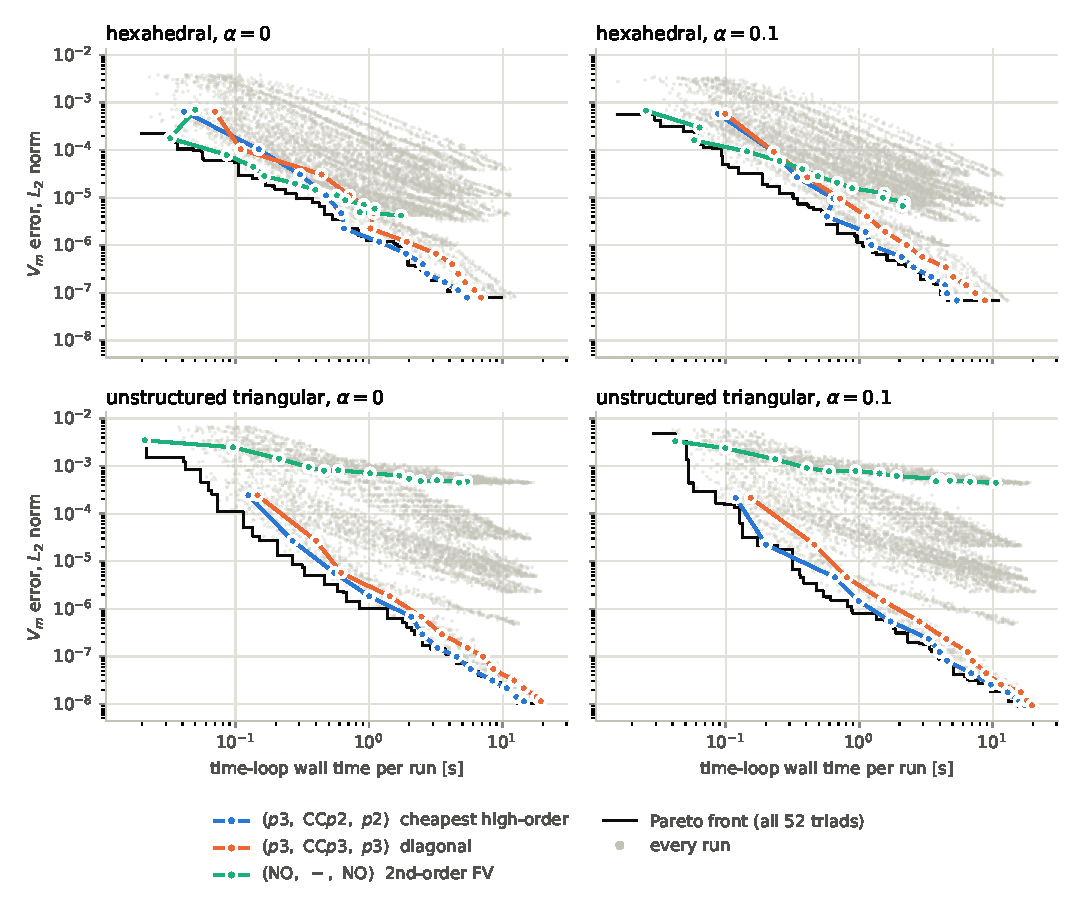
\includegraphics[width=\linewidth]{figures/fig_pareto_triads.pdf}
  \caption{Accuracy--cost Pareto front over the $(\Vm, \text{states},
  \Iion)$ triad space, from the $\code{np}=4$ sweep with Picard and
  $\Delta t=10^{-3}$, $N=10$--$130$. Each faint dot is one run; the black step
  curve is the non-dominated front; the three coloured curves are
  mesh-refinement paths for the cheapest high-order triad
  $(p3,\mathrm{CC}p2,p2)$, the diagonal $(p3,\mathrm{CC}p3,p3)$, and
  second-order FV. The diagonal triad lies above the front in all four panels.
  Generated by \code{figures/fig\_pareto\_triads.py} from
  \code{figures/pareto\_2d\_picard\_dt1e-3.csv}.}
  \label{fig:pareto-triads}
\end{figure}

\paragraph{The 3-D sweep, and what it replicates.} The 3-D study is a sweep of
its own: seven triads on hexahedral and unstructured tetrahedral meshes,
$N=10$--$30$, BDF4 with the ESDIRK3 startup and $\Delta t=10^{-3}$. Its orders,
and the 2-D ones, are Figure~\ref{fig:order-vm}. Two results carry over from 2-D
unchanged. The loss of consistency of the standard operator on simplices is
\emph{worse} in 3-D --- \code{NO} fits $0.65$ on tetrahedra against $0.77$ on
triangles and $1.96$--$1.98$ on hexahedra --- and the cheap triad still matches
the diagonal, $3.383$ for $(p3,\mathrm{CC}p2,p2)$ against $3.381$ for
$(p3,\mathrm{CC}p3,p3)$.

One number must be read with care: $p3$ fits $3.38$ in 3-D against $3.72$--$4.32$
in 2-D, and that is \emph{not} temporal contamination. Halving $\Delta t$ on the
finest 3-D mesh moves the error in the seventh digit
($3.9486606\times10^{-5}\to3.9486604\times10^{-5}$ on hexa), so the temporal
error is $\sim10^{-11}$ against a spatial error of $\sim3\times10^{-5}$. The
pairwise orders say the two families are in different regimes: on hexahedra they
oscillate without rising ($3.67, 3.22, 3.20, 3.35$) while on tetrahedra they
climb monotonically ($2.91, 3.15, 3.40, 3.51$), i.e. the asymptotic range is not
reached by $N=30$ --- and $N>30$ is out of reach here, since $N=50$ on hexahedra
is killed by the OOM killer during stiffness assembly with four ranks.

\begin{figure}[htbp]
  \centering
  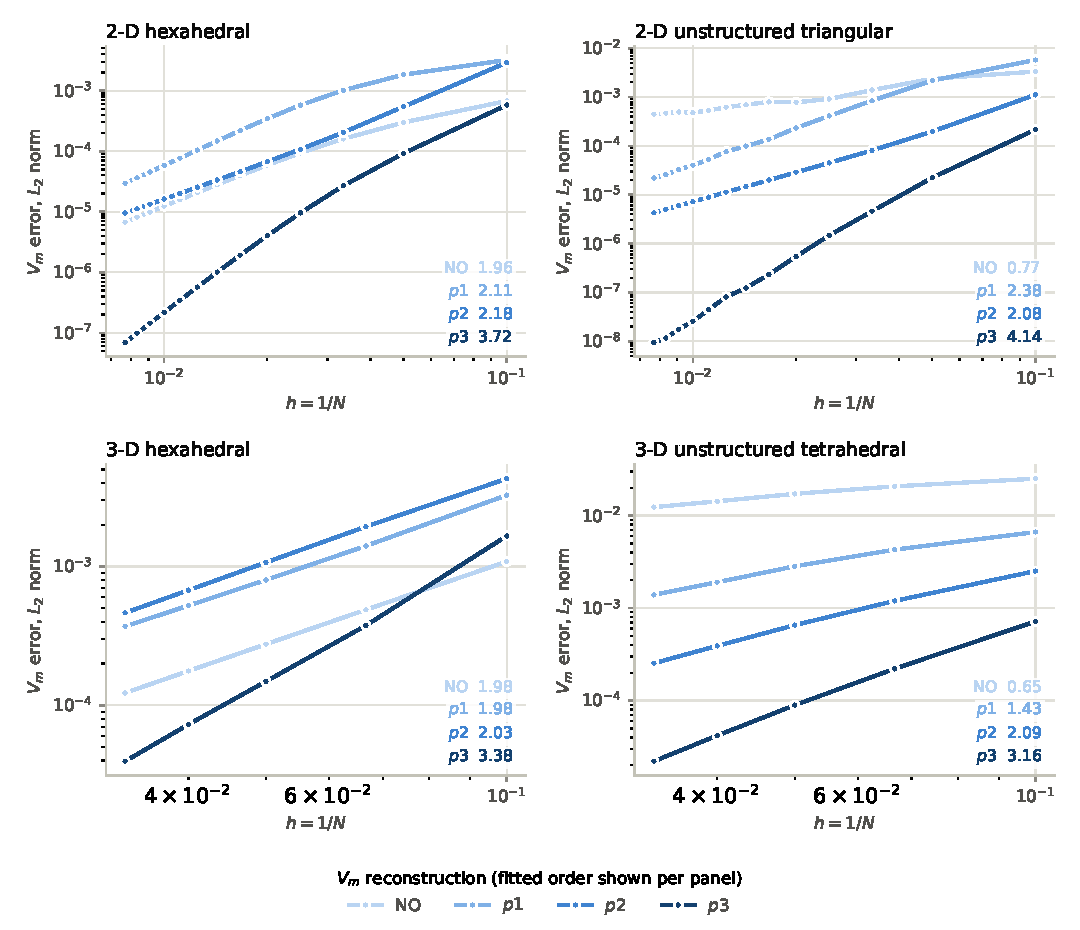
\includegraphics[width=\linewidth]{figures/fig_order_vm.pdf}
  \caption{Spatial order of $\Vm$ for the four reconstruction levels on the
  diagonal, in 2-D ($N=10$--$130$) and 3-D ($N=10$--$30$), on structured and
  unstructured meshes. The number in each panel is the order fitted over that
  panel's whole range. The four levels are an ordered scale, so they are drawn
  as one hue light to dark rather than as four categorical colours. Generated by
  \code{figures/fig\_orders.py} from the raw \code{errors\_vs\_N} files.}
  \label{fig:order-vm}
\end{figure}

\paragraph{States at cell centres against states at Gauss points.} The claim
that the cell-centred mode is both cheaper and strictly more accurate is
Figure~\ref{fig:cc-vs-gp}, and it now holds in 3-D as well. Integrating the
states at the quadrature points pins their cell-centred error at order two
exactly --- $2.00$ and $1.99$ in 2-D, $1.99$ and $1.92$ in 3-D --- because
averaging them back to the centres destroys the order, while the cell-centred
mode follows the scheme ($3.48$, $3.87$, $3.25$, $2.97$). $\Vm$ itself converges
identically either way ($3.384$ against $3.381$ on 3-D hexa), so nothing is lost
by the cheaper path, which solves one ODE per cell instead of $N_q$.

\begin{figure}[htbp]
  \centering
  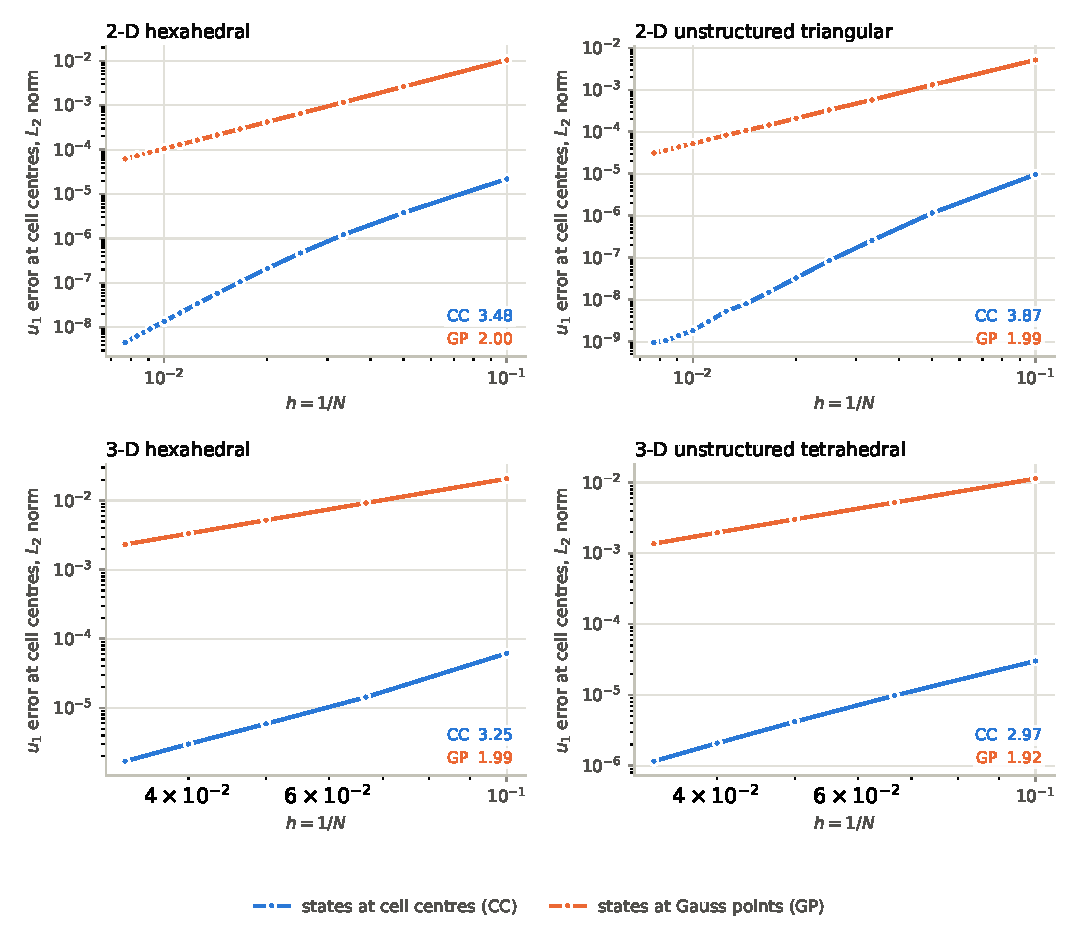
\includegraphics[width=\linewidth]{figures/fig_cc_vs_gp.pdf}
  \caption{Error of the ionic state $u_1$ at cell centres,
  \code{cellCentredReconstruct} against \code{gaussPointODE}, with the
  $(p3,\cdot,p3)$ triad. The Gauss-point mode is pinned at order two in every
  panel; the cell-centred mode follows the scheme. Generated by
  \code{figures/fig\_orders.py}.}
  \label{fig:cc-vs-gp}
\end{figure}

\paragraph{Only odd reconstruction degrees buy a new order.}
Fixing the hexahedral mesh, $\alpha=0$, and $\Delta t=10^{-3}$, the observed
order of $\Vm$ in the fine fit ($N=70$--$100$) is
\begin{center}
\begin{tabular}{@{}lcccc@{}}
\toprule
$\Vm$ reconstruction & \code{NO} & \code{p1} & \code{p2} & \code{p3} \\
\midrule
Expected order (\S\ref{sec:lre}) & 2 & 2 & 3 & 4 \\
Observed order (hexa) & $2.00$ & $2.61$ & $2.03$ & $4.32$ \\
Observed order (triangular unstr) & $0.96$ & $2.60$ & $1.99$ & $4.48$ \\
\bottomrule
\end{tabular}
\end{center}
The pattern is the classical odd/even one for cell-centred diffusion operators:
the reconstructed face gradient has $O(h^{N})$ truncation for degree $N$, but on
approximately symmetric stencils the even-order error term cancels, so odd
degrees gain one extra order and even degrees do not. This reproduces $2$, $2$,
and $4$ for \code{p1}, \code{p2}, and \code{p3}, and explains why \code{p2} does
\emph{not} reach the nominal third order anticipated in \S\ref{sec:lre}: in the
fine fit \code{p2} delivers $2.03$, barely above \code{p1} but with a wider
stencil and a higher cost. The practical conclusion is that, for this operator,
the useful options are \code{p1} and \code{p3}; \code{p2} pays for a wider
stencil without buying order.

\paragraph{The standard operator loses consistency on the unstructured mesh.}
With \code{useHighOrder\_Vm=false} the observed order on the unstructured
triangular mesh drops to $0.96$ (and to $0.80$ in the broad $N=10$--$100$ fit),
against $2.00$ on the hexahedral one. The reason is the one noted in
\S\ref{sec:std-operator}: the solver assembles only the orthogonal part of the
face flux, and on a triangular mesh with significant non-orthogonality the
omitted term is not a high-order perturbation but a leading-order contribution.
Stabilisation does not fix it ($0.95$ with $\alpha=0.1$). By contrast, the
cheapest LRE reconstruction, \code{p1}, recovers $2.60$ on that same mesh, and
\code{p3} reaches $4.48$. This is the strongest quantitative argument in the
report in favour of the high-order path: on unstructured meshes the LRE does not
merely improve the order, it restores the consistency that the standard operator
loses.

\paragraph{The bottleneck moves to the ionic path once $\Vm$ is high order.}
With \code{NO} or \code{p1} for $\Vm$, the complete $5\times4$ grid of
(states $\times$ $\Iion$) combinations gives the same order to three digits:
$2.000$ and $2.611$ respectively. The ionic path is then irrelevant. With
\code{p3} the picture changes completely (hexa mesh, $\alpha=0$,
$\Delta t=10^{-3}$, order of $\Vm$ in the fine fit):
\begin{center}
\begin{tabular}{@{}lcccc@{}}
\toprule
states $\backslash$ $\Iion$ & \code{NO} & \code{p1} & \code{p2} & \code{p3} \\
\midrule
\code{na}   & $2.01$ & --     & --     & --     \\
\code{CCp1} & --     & $2.02$ & $2.12$ & $2.12$ \\
\code{CCp2} & --     & $2.02$ & $\mathbf{4.32}$ & $\mathbf{4.32}$ \\
\code{CCp3} & --     & $2.02$ & $\mathbf{4.32}$ & $\mathbf{4.32}$ \\
\code{GP}   & --     & $2.02$ & $\mathbf{4.32}$ & $\mathbf{4.32}$ \\
\bottomrule
\end{tabular}
\end{center}
Fourth order is unlocked if and only if the $\Iion$ quadrature is at least
\code{p2} \emph{and} the state interpolator is at least \code{CCp2}. Failing
either condition degrades the result to second order, even though the $\Vm$
reconstruction is cubic and the diffusion operator is assembled to fourth order.
This is the quantitative verification of the principle stated in
\S\ref{sec:lre}: the observed order is the minimum of the orders of all the
links. Translated into a usage rule, the triplet must be raised jointly:
\code{p3--CCp2--p2} is the cheapest configuration that attains fourth order, and
raising only one of the three levels is wasted effort.

\paragraph{\code{cellCentredReconstruct} dominates \code{gaussPointODE}.}
The legacy \code{GP} mode reaches $4.19$ on the quadrature-point metrics
$u_1^G$ and $u_2^G$, but its cell-centred state errors are stuck at $2.000$:
averaging the states from the quadrature points back to the cell centres
destroys the order, exactly as anticipated in \S\ref{sec:iion-quad}. The default
mode \code{CCp3} delivers $4.08$ at cell centres and $4.28$ at the quadrature
points simultaneously, and does so integrating one ODE per cell instead of one
per quadrature point. On the quadrature-point metrics, the degree of the state
interpolator sets the order directly: \code{CCp1}$\to2.15$,
\code{CCp2}$\to3.00$, \code{CCp3}$\to4.28$. There is no metric on which
\code{GP} beats \code{CCp3}.

\paragraph{With $\Delta t=10^{-2}$ the temporal floor contaminates the state
rates.}
For the \code{p3--CCp2--p2} triplet on the hexa mesh, the cell-centred $L_2$
error of $u_1$ goes from $9.68\times10^{-8}$ ($N=70$) to $7.47\times10^{-8}$
($N=100$) with $\Delta t=10^{-2}$: it has stalled. With $\Delta t=10^{-3}$ the
same two points give $6.71\times10^{-8}$ and $1.57\times10^{-8}$, i.e.\ it is
still converging at fourth order. The Crank--Nicolson error plus that of the
linear $\Vm$ ramp in $\tau$, \eqref{eq:ode-vm-interpolation}, produces a floor of
$\approx7\times10^{-8}$ that the fine meshes already reach. Quantified over the
whole 2D sweep, the fine fit changes by more than $0.5$ when going from
$\Delta t=10^{-2}$ to $10^{-3}$ in $120$ out of $156$ \code{p3} configurations
for $u_1$ and $u_2$, and in $36$ out of $156$ for $\Vm$. \textbf{The $u_1$ and
$u_2$ rates of the 2D tables with $\Delta t=10^{-2}$ must not be read as spatial
orders}; only the $\Delta t=10^{-3}$ tables are. For $\Vm$, whose error is
larger, the contamination is marginal.

\paragraph{Stabilisation is unnecessary in 2D.}
Except for the \code{NO} case on the hexahedral mesh, where $\alpha=0.1$
artificially raises the fine fit from $2.00$ to $2.29$ (a pre-asymptotic effect,
not an order improvement), the median effect of going from $\alpha=0$ to
$\alpha=0.1$ on the order of $\Vm$ is smaller than $0.05$ in every other
level/mesh combination. Since $\alpha>0$ additionally adds terms to the assembly
and raises the run time by between $40\%$ and $80\%$, $\alpha=0$ is the
preferable choice in 2D.

\subsection{Three-dimensional manufactured problem}
\label{sec:en-results-3d}
The tables in this subsection are generated directly from the
current \path{/home/pablo/OpenFOAM/pablo-v2312/run/tutorials_electro/highOrderManufacturedFDAImplicitPETSc/results/example0} result tree. The method-specific roots are \path{/home/pablo/OpenFOAM/pablo-v2312/run/tutorials_electro/highOrderManufacturedFDAImplicitPETSc/results/example0/3D_CN_cons_Picard_RKF45}, \path{/home/pablo/OpenFOAM/pablo-v2312/run/tutorials_electro/highOrderManufacturedFDAImplicitPETSc/results/example0/3D_CN_cons_diagonalIion_RKF45}, \path{/home/pablo/OpenFOAM/pablo-v2312/run/tutorials_electro/highOrderManufacturedFDAImplicitPETSc/results/example0/3D_CN_cons_JFNK_RKF45}.
All entries use \code{crankNicolson}, the \code{consistent} mass matrix, and \code{RKF45} for the state ODEs.
The first column reports \code{Vm-states-Iion}: the $V_m$ reconstruction degree, the state treatment (\code{CCp*}, \code{GP}, or \code{na}), and the $\Iion$ quadrature/reconstruction setting.
Fits use $N=10$--$30$ for the broad mesh range and $N=20$--$30$ for the fine-mesh range.
The last two columns audit the nonlinear solver: \code{RB} counts rolled-back steps and $n_{\mathrm{nl}}$ summarises the nonlinear iterations per step (median/maximum).

\subsubsection{\code{Picard}}
\paragraph{$\Delta t=10^{-2}$}
\tiny
\setlength{\tabcolsep}{1.4pt}
\begin{longtable}{lllrrrrrrrrrrrrrrrr}
\caption{3D manufactured results for \code{Picard}, \code{crankNicolson}, \code{consistent} mass, \code{RKF45} states, and $\Delta t=10^{-2}$. The first convergence block is fitted over $N=10$--$30$; the second over $N=20$--$30$. The first column records the actual \code{Vm-states-Iion} triplet used by the run. \textbf{RB} is the number of time steps that exhausted the nonlinear iteration budget, accumulated over the 21 mesh sizes of the row (105 time steps per row in total). \code{Picard} accepts its last iterate with a warning instead of rolling back, so for this method the column counts steps accepted without converging. \textbf{$n_{\mathrm{nl}}$} reports the median and the maximum number of nonlinear iterations per step over those same steps; the configured budget is \code{nonlinearIterations}$=2000$.}\label{tab:en-results-3d-picard-1p0em02}\\
\toprule
& & & \multicolumn{6}{c}{Fit $N=10$--$30$} & \multicolumn{6}{c}{Fit $N=20$--$30$} & & & & \\
\cmidrule(lr){4-9}\cmidrule(lr){10-15}
\code{Vm-states-Iion} & Mesh type & $\alpha$ & $V_m$ & $V_m^G$ & $u_1$ & $u_1^G$ & $u_2$ & $u_2^G$ & $V_m$ & $V_m^G$ & $u_1$ & $u_1^G$ & $u_2$ & $u_2^G$ & $t_{\Sigma}$ [s] & RSS$_{\Sigma}$ [MB] & RB & $n_{\mathrm{nl}}$ \\
\midrule
\endfirsthead
\toprule
& & & \multicolumn{6}{c}{Fit $N=10$--$30$} & \multicolumn{6}{c}{Fit $N=20$--$30$} & & & & \\
\cmidrule(lr){4-9}\cmidrule(lr){10-15}
\code{Vm-states-Iion} & Mesh type & $\alpha$ & $V_m$ & $V_m^G$ & $u_1$ & $u_1^G$ & $u_2$ & $u_2^G$ & $V_m$ & $V_m^G$ & $u_1$ & $u_1^G$ & $u_2$ & $u_2^G$ & $t_{\Sigma}$ [s] & RSS$_{\Sigma}$ [MB] & RB & $n_{\mathrm{nl}}$ \\
\midrule
\endhead
\code{NO--na--NO} & hexa & 0.0 & 1.985 & 1.985 & 1.994 & 1.994 & 1.994 & 1.994 & 1.993 & 1.993 & 2.009 & 2.009 & 2.009 & 2.009 & 13.701 & 4034.4 & 0 & 4.00/4 \\
\code{NO--na--NO} & hexa & 0.1 & 1.436 & 1.436 & 1.297 & 1.297 & 1.306 & 1.306 & 1.411 & 1.411 & 1.214 & 1.214 & 1.223 & 1.223 & 22.097 & 6312.2 & 0 & 4.00/4 \\
\code{NO--na--NO} & tetra unstr & 0.0 & 0.664 & 0.664 & 0.375 & 0.375 & 0.373 & 0.373 & 0.826 & 0.826 & 0.617 & 0.617 & 0.616 & 0.616 & 21.144 & 4988.3 & 0 & 4.00/5 \\
\code{NO--na--NO} & tetra unstr & 0.1 & 0.677 & 0.677 & 0.398 & 0.398 & 0.396 & 0.396 & 0.823 & 0.823 & 0.629 & 0.629 & 0.628 & 0.628 & 105.72 & 12055.9 & 0 & 4.00/5 \\
\hline
\code{NO--CCp1--p1} & hexa & 0.0 & 1.985 & 1.985 & 1.998 & 2.166 & 1.995 & 2.246 & 1.992 & 1.992 & 2.010 & 2.208 & 2.009 & 2.189 & 28.255 & 4710.5 & 0 & 4.00/4 \\
\code{NO--CCp1--p1} & hexa & 0.1 & 1.436 & 1.436 & 1.287 & 2.167 & 1.306 & 2.230 & 1.411 & 1.411 & 1.205 & 2.208 & 1.224 & 2.159 & 46.542 & 6565.3 & 0 & 4.00/4 \\
\code{NO--CCp1--p1} & tetra unstr & 0.0 & 0.664 & 0.664 & 0.375 & 0.375 & 0.373 & 0.373 & 0.826 & 0.826 & 0.617 & 0.617 & 0.616 & 0.616 & 116.61 & 6199.0 & 0 & 4.00/5 \\
\code{NO--CCp1--p1} & tetra unstr & 0.1 & 0.677 & 0.677 & 0.398 & 0.398 & 0.396 & 0.396 & 0.823 & 0.823 & 0.629 & 0.629 & 0.628 & 0.628 & 186.46 & 12250.5 & 0 & 4.00/5 \\
\hline
\code{NO--CCp1--p2} & hexa & 0.0 & 1.985 & 1.985 & 1.999 & 2.098 & 1.994 & 2.090 & 1.992 & 1.992 & 2.011 & 2.130 & 2.009 & 2.062 & 31.539 & 5888.2 & 0 & 4.00/4 \\
\code{NO--CCp1--p2} & hexa & 0.1 & 1.436 & 1.436 & 1.283 & 2.098 & 1.307 & 2.087 & 1.411 & 1.411 & 1.201 & 2.130 & 1.224 & 2.056 & 44.590 & 7233.9 & 0 & 4.00/4 \\
\code{NO--CCp1--p2} & tetra unstr & 0.0 & 0.664 & 0.664 & 0.375 & 1.924 & 0.373 & 0.457 & 0.826 & 0.826 & 0.617 & 1.896 & 0.616 & 0.669 & 128.54 & 6649.6 & 0 & 4.00/5 \\
\code{NO--CCp1--p2} & tetra unstr & 0.1 & 0.677 & 0.677 & 0.398 & 1.928 & 0.396 & 0.483 & 0.823 & 0.823 & 0.629 & 1.903 & 0.628 & 0.683 & 199.14 & 12498.6 & 0 & 4.00/5 \\
\hline
\code{NO--CCp1--p3} & hexa & 0.0 & 1.985 & 1.985 & 1.999 & 2.094 & 1.994 & 2.088 & 1.992 & 1.992 & 2.011 & 2.127 & 2.009 & 2.061 & 35.704 & 8248.0 & 0 & 4.00/4 \\
\code{NO--CCp1--p3} & hexa & 0.1 & 1.436 & 1.436 & 1.283 & 2.095 & 1.307 & 2.085 & 1.411 & 1.411 & 1.201 & 2.127 & 1.224 & 2.054 & 57.374 & 9568.3 & 0 & 4.00/4 \\
\code{NO--CCp1--p3} & tetra unstr & 0.0 & 0.664 & 0.664 & 0.375 & 1.923 & 0.373 & 0.460 & 0.826 & 0.826 & 0.617 & 1.906 & 0.616 & 0.670 & 123.28 & 7555.6 & 0 & 4.00/5 \\
\code{NO--CCp1--p3} & tetra unstr & 0.1 & 0.677 & 0.677 & 0.398 & 1.926 & 0.396 & 0.485 & 0.823 & 0.823 & 0.629 & 1.912 & 0.628 & 0.684 & 217.11 & 12994.2 & 0 & 4.00/5 \\
\hline
\code{NO--CCp2--p1} & hexa & 0.0 & 1.977 & 1.977 & 2.009 & 3.171 & 1.987 & 2.618 & 1.989 & 1.989 & 2.014 & 3.091 & 2.005 & 2.390 & 37.567 & 5489.6 & 0 & 4.00/4 \\
\code{NO--CCp2--p1} & hexa & 0.1 & 1.447 & 1.447 & 1.257 & 3.172 & 1.318 & 2.180 & 1.426 & 1.426 & 1.176 & 3.092 & 1.239 & 1.626 & 56.054 & 6775.8 & 0 & 4.00/4 \\
\code{NO--CCp2--p1} & tetra unstr & 0.0 & 0.664 & 0.664 & 0.375 & 0.375 & 0.373 & 0.373 & 0.826 & 0.826 & 0.617 & 0.617 & 0.616 & 0.616 & 190.82 & 9543.3 & 0 & 4.00/5 \\
\code{NO--CCp2--p1} & tetra unstr & 0.1 & 0.677 & 0.677 & 0.398 & 0.398 & 0.396 & 0.396 & 0.823 & 0.823 & 0.629 & 0.629 & 0.628 & 0.628 & 244.84 & 13294.2 & 0 & 4.00/5 \\
\hline
\code{NO--CCp2--p2} & hexa & 0.0 & 1.969 & 1.969 & 2.010 & 3.247 & 1.979 & 2.753 & 1.985 & 1.985 & 2.013 & 3.146 & 2.001 & 2.494 & 55.354 & 6662.9 & 0 & 4.00/4 \\
\code{NO--CCp2--p2} & hexa & 0.1 & 1.457 & 1.457 & 1.248 & 3.248 & 1.333 & 2.320 & 1.441 & 1.441 & 1.170 & 3.147 & 1.257 & 1.718 & 58.989 & 7953.8 & 0 & 4.00/4 \\
\code{NO--CCp2--p2} & tetra unstr & 0.0 & 0.664 & 0.664 & 0.375 & 2.080 & 0.373 & 0.465 & 0.826 & 0.826 & 0.617 & 1.273 & 0.616 & 0.673 & 183.95 & 9999.5 & 0 & 4.00/5 \\
\code{NO--CCp2--p2} & tetra unstr & 0.1 & 0.677 & 0.677 & 0.398 & 2.128 & 0.396 & 0.486 & 0.823 & 0.823 & 0.629 & 1.333 & 0.628 & 0.683 & 257.01 & 13767.7 & 0 & 4.00/5 \\
\hline
\code{NO--CCp2--p3} & hexa & 0.0 & 1.969 & 1.969 & 2.010 & 3.252 & 1.979 & 2.758 & 1.985 & 1.985 & 2.013 & 3.149 & 2.001 & 2.501 & 68.040 & 9017.1 & 0 & 4.00/4 \\
\code{NO--CCp2--p3} & hexa & 0.1 & 1.457 & 1.457 & 1.248 & 3.253 & 1.333 & 2.328 & 1.441 & 1.441 & 1.170 & 3.150 & 1.257 & 1.726 & 66.357 & 10307.2 & 0 & 4.00/4 \\
\code{NO--CCp2--p3} & tetra unstr & 0.0 & 0.664 & 0.664 & 0.375 & 1.992 & 0.373 & 0.466 & 0.826 & 0.826 & 0.617 & 1.241 & 0.616 & 0.675 & 180.62 & 10904.7 & 0 & 4.00/5 \\
\code{NO--CCp2--p3} & tetra unstr & 0.1 & 0.677 & 0.677 & 0.398 & 2.039 & 0.396 & 0.487 & 0.823 & 0.823 & 0.629 & 1.295 & 0.628 & 0.686 & 257.54 & 14649.4 & 0 & 4.00/5 \\
\hline
\code{NO--CCp3--p1} & hexa & 0.0 & 1.980 & 1.980 & 2.001 & 4.033 & 1.989 & 2.062 & 1.991 & 1.991 & 2.011 & 4.072 & 2.007 & 2.017 & 90.356 & 7390.4 & 0 & 4.00/4 \\
\code{NO--CCp3--p1} & hexa & 0.1 & 1.452 & 1.452 & 1.244 & 4.015 & 1.323 & 1.276 & 1.429 & 1.429 & 1.170 & 4.028 & 1.241 & 1.186 & 89.988 & 8677.1 & 0 & 4.00/4 \\
\code{NO--CCp3--p1} & tetra unstr & 0.0 & 0.664 & 0.664 & 0.375 & 0.375 & 0.373 & 0.373 & 0.826 & 0.826 & 0.617 & 0.617 & 0.616 & 0.616 & 358.12 & 18313.3 & 0 & 4.00/5 \\
\code{NO--CCp3--p1} & tetra unstr & 0.1 & 0.677 & 0.677 & 0.398 & 0.398 & 0.396 & 0.396 & 0.823 & 0.823 & 0.629 & 0.629 & 0.628 & 0.628 & 385.12 & 22079.8 & 0 & 4.00/5 \\
\hline
\code{NO--CCp3--p2} & hexa & 0.0 & 1.976 & 1.976 & 2.000 & 3.980 & 1.985 & 2.107 & 1.990 & 1.990 & 2.011 & 4.053 & 2.005 & 2.022 & 94.372 & 8563.2 & 0 & 4.00/4 \\
\code{NO--CCp3--p2} & hexa & 0.1 & 1.469 & 1.469 & 1.233 & 3.966 & 1.343 & 1.305 & 1.447 & 1.447 & 1.163 & 4.019 & 1.261 & 1.187 & 88.556 & 9854.5 & 0 & 4.00/4 \\
\code{NO--CCp3--p2} & tetra unstr & 0.0 & 0.664 & 0.664 & 0.375 & 0.890 & 0.373 & 0.418 & 0.826 & 0.826 & 0.617 & 0.674 & 0.616 & 0.657 & 346.61 & 18765.0 & 0 & 4.00/5 \\
\code{NO--CCp3--p2} & tetra unstr & 0.1 & 0.677 & 0.677 & 0.398 & 0.930 & 0.396 & 0.441 & 0.823 & 0.823 & 0.629 & 0.689 & 0.628 & 0.670 & 399.32 & 22514.1 & 0 & 4.00/5 \\
\hline
\code{NO--CCp3--p3} & hexa & 0.0 & 1.976 & 1.976 & 2.000 & 3.973 & 1.985 & 2.108 & 1.990 & 1.990 & 2.011 & 4.054 & 2.005 & 2.022 & 94.607 & 10920.3 & 0 & 4.00/4 \\
\code{NO--CCp3--p3} & hexa & 0.1 & 1.469 & 1.469 & 1.233 & 3.959 & 1.343 & 1.305 & 1.447 & 1.447 & 1.163 & 4.021 & 1.261 & 1.186 & 106.47 & 12209.7 & 0 & 4.00/4 \\
\code{NO--CCp3--p3} & tetra unstr & 0.0 & 0.664 & 0.664 & 0.375 & 0.888 & 0.373 & 0.432 & 0.826 & 0.826 & 0.617 & 0.684 & 0.616 & 0.665 & 348.72 & 19672.6 & 0 & 4.00/5 \\
\code{NO--CCp3--p3} & tetra unstr & 0.1 & 0.677 & 0.677 & 0.398 & 0.926 & 0.396 & 0.454 & 0.823 & 0.823 & 0.629 & 0.697 & 0.628 & 0.677 & 418.61 & 23417.4 & 0 & 4.00/5 \\
\hline
\code{NO--GP--p1} & hexa & 0.0 & 1.984 & 1.984 & 1.992 & 2.072 & 1.992 & 2.077 & 1.992 & 1.992 & 1.996 & 2.038 & 1.997 & 2.041 & 28.095 & 4465.1 & 0 & 4.00/4 \\
\code{NO--GP--p1} & hexa & 0.1 & 1.459 & 1.459 & 1.992 & 2.073 & 1.993 & 2.079 & 1.429 & 1.429 & 1.996 & 2.038 & 1.996 & 2.041 & 37.380 & 6564.9 & 0 & 4.00/4 \\
\code{NO--GP--p1} & tetra unstr & 0.0 & 0.664 & 0.664 & 0.375 & 0.375 & 0.373 & 0.373 & 0.826 & 0.826 & 0.617 & 0.617 & 0.616 & 0.616 & 29.082 & 5234.8 & 0 & 4.00/5 \\
\code{NO--GP--p1} & tetra unstr & 0.1 & 0.677 & 0.677 & 0.398 & 0.398 & 0.396 & 0.396 & 0.823 & 0.823 & 0.629 & 0.629 & 0.628 & 0.628 & 97.186 & 12251.2 & 0 & 4.00/5 \\
\hline
\code{NO--GP--p2} & hexa & 0.0 & 1.983 & 1.983 & 1.984 & 2.014 & 1.985 & 2.018 & 1.992 & 1.992 & 1.992 & 2.007 & 1.993 & 2.009 & 72.453 & 5644.5 & 0 & 4.00/4 \\
\code{NO--GP--p2} & hexa & 0.1 & 1.482 & 1.482 & 1.984 & 2.015 & 1.985 & 2.018 & 1.447 & 1.447 & 1.992 & 2.007 & 1.993 & 2.010 & 84.100 & 7214.1 & 0 & 4.00/4 \\
\code{NO--GP--p2} & tetra unstr & 0.0 & 0.664 & 0.664 & 1.832 & 0.861 & 0.516 & 0.859 & 0.826 & 0.826 & 1.792 & 0.867 & 0.652 & 0.866 & 43.013 & 5699.3 & 0 & 4.00/5 \\
\code{NO--GP--p2} & tetra unstr & 0.1 & 0.677 & 0.677 & 1.844 & 0.883 & 0.546 & 0.881 & 0.823 & 0.823 & 1.812 & 0.884 & 0.668 & 0.883 & 115.92 & 12501.1 & 0 & 4.00/5 \\
\hline
\code{NO--GP--p3} & hexa & 0.0 & 1.983 & 1.983 & 1.983 & 2.010 & 1.984 & 2.014 & 1.992 & 1.992 & 1.992 & 2.005 & 1.993 & 2.008 & 159.70 & 7997.1 & 0 & 4.00/4 \\
\code{NO--GP--p3} & hexa & 0.1 & 1.482 & 1.482 & 1.984 & 2.011 & 1.985 & 2.015 & 1.447 & 1.447 & 1.992 & 2.006 & 1.992 & 2.008 & 156.73 & 9198.0 & 0 & 4.00/4 \\
\code{NO--GP--p3} & tetra unstr & 0.0 & 0.664 & 0.664 & 1.828 & 0.863 & 0.513 & 0.862 & 0.826 & 0.826 & 1.790 & 0.868 & 0.651 & 0.868 & 71.823 & 6602.5 & 0 & 4.00/5 \\
\code{NO--GP--p3} & tetra unstr & 0.1 & 0.677 & 0.677 & 1.840 & 0.885 & 0.542 & 0.884 & 0.823 & 0.823 & 1.810 & 0.885 & 0.667 & 0.885 & 146.28 & 12996.8 & 0 & 4.00/5 \\
\hline
\code{p1--na--NO} & hexa & 0.0 & 1.967 & 2.095 & 1.927 & 1.927 & 1.930 & 1.930 & 1.919 & 2.125 & 1.838 & 1.838 & 1.845 & 1.845 & 77.496 & 7145.3 & 0 & 4.00/4 \\
\code{p1--na--NO} & hexa & 0.1 & 2.067 & 2.093 & 2.047 & 2.047 & 2.048 & 2.048 & 2.066 & 2.124 & 2.033 & 2.033 & 2.035 & 2.035 & 67.389 & 8698.8 & 0 & 4.00/4 \\
\code{p1--na--NO} & tetra unstr & 0.0 & 1.474 & 1.866 & 1.140 & 1.140 & 1.142 & 1.142 & 1.771 & 1.928 & 1.419 & 1.419 & 1.428 & 1.428 & 207.91 & 9888.9 & 0 & 4.00/4 \\
\code{p1--na--NO} & tetra unstr & 0.1 & 1.613 & 1.909 & 1.262 & 1.262 & 1.264 & 1.264 & 1.889 & 1.963 & 1.556 & 1.556 & 1.558 & 1.558 & 209.36 & 11566.5 & 0 & 4.00/4 \\
\hline
\code{p1--CCp1--p1} & hexa & 0.0 & 1.967 & 2.095 & 1.926 & 2.166 & 1.930 & 2.193 & 1.919 & 2.125 & 1.836 & 2.207 & 1.845 & 2.115 & 73.944 & 7263.0 & 0 & 4.00/4 \\
\code{p1--CCp1--p1} & hexa & 0.1 & 2.067 & 2.093 & 2.046 & 2.167 & 2.048 & 2.225 & 2.066 & 2.124 & 2.033 & 2.208 & 2.035 & 2.168 & 93.736 & 8854.4 & 0 & 4.00/4 \\
\code{p1--CCp1--p1} & tetra unstr & 0.0 & 1.474 & 1.866 & 1.140 & 1.140 & 1.142 & 1.142 & 1.771 & 1.928 & 1.419 & 1.419 & 1.428 & 1.428 & 315.13 & 10862.6 & 0 & 4.00/4 \\
\code{p1--CCp1--p1} & tetra unstr & 0.1 & 1.613 & 1.909 & 1.262 & 1.262 & 1.264 & 1.264 & 1.889 & 1.963 & 1.556 & 1.556 & 1.558 & 1.558 & 289.28 & 12081.8 & 0 & 4.00/4 \\
\hline
\code{p1--CCp1--p2} & hexa & 0.0 & 1.967 & 2.095 & 1.925 & 2.098 & 1.930 & 2.083 & 1.919 & 2.125 & 1.835 & 2.130 & 1.845 & 2.049 & 83.398 & 8101.2 & 0 & 4.00/4 \\
\code{p1--CCp1--p2} & hexa & 0.1 & 2.067 & 2.093 & 2.046 & 2.098 & 2.047 & 2.090 & 2.066 & 2.124 & 2.033 & 2.130 & 2.035 & 2.061 & 87.516 & 9506.3 & 0 & 4.00/4 \\
\code{p1--CCp1--p2} & tetra unstr & 0.0 & 1.474 & 1.866 & 1.139 & 1.973 & 1.142 & 1.493 & 1.771 & 1.928 & 1.419 & 1.984 & 1.428 & 1.590 & 330.99 & 11305.1 & 0 & 4.00/4 \\
\code{p1--CCp1--p2} & tetra unstr & 0.1 & 1.613 & 1.909 & 1.262 & 1.973 & 1.264 & 1.621 & 1.889 & 1.963 & 1.556 & 1.983 & 1.558 & 1.721 & 309.50 & 12482.1 & 0 & 4.00/4 \\
\hline
\code{p1--CCp1--p3} & hexa & 0.0 & 1.967 & 2.095 & 1.925 & 2.094 & 1.930 & 2.081 & 1.919 & 2.125 & 1.835 & 2.127 & 1.845 & 2.048 & 105.81 & 10456.5 & 0 & 4.00/4 \\
\code{p1--CCp1--p3} & hexa & 0.1 & 2.067 & 2.093 & 2.046 & 2.094 & 2.047 & 2.088 & 2.066 & 2.124 & 2.033 & 2.127 & 2.035 & 2.060 & 106.65 & 11155.3 & 0 & 4.00/4 \\
\code{p1--CCp1--p3} & tetra unstr & 0.0 & 1.474 & 1.866 & 1.139 & 1.965 & 1.142 & 1.505 & 1.771 & 1.928 & 1.419 & 1.982 & 1.428 & 1.597 & 307.94 & 12243.6 & 0 & 4.00/4 \\
\code{p1--CCp1--p3} & tetra unstr & 0.1 & 1.613 & 1.909 & 1.262 & 1.965 & 1.264 & 1.632 & 1.889 & 1.963 & 1.556 & 1.982 & 1.558 & 1.727 & 309.45 & 13293.2 & 0 & 4.00/4 \\
\hline
\code{p1--CCp2--p1} & hexa & 0.0 & 1.966 & 2.095 & 1.926 & 3.169 & 1.929 & 2.043 & 1.919 & 2.125 & 1.831 & 3.089 & 1.845 & 1.844 & 115.71 & 7558.1 & 0 & 4.00/4 \\
\code{p1--CCp2--p1} & hexa & 0.1 & 2.065 & 2.093 & 2.050 & 3.170 & 2.046 & 2.200 & 2.066 & 2.124 & 2.033 & 3.090 & 2.034 & 2.090 & 96.811 & 8857.6 & 0 & 4.00/4 \\
\code{p1--CCp2--p1} & tetra unstr & 0.0 & 1.474 & 1.866 & 1.140 & 1.140 & 1.142 & 1.142 & 1.771 & 1.928 & 1.419 & 1.419 & 1.428 & 1.428 & 356.84 & 14195.6 & 0 & 4.00/4 \\
\code{p1--CCp2--p1} & tetra unstr & 0.1 & 1.613 & 1.909 & 1.262 & 1.262 & 1.264 & 1.264 & 1.889 & 1.963 & 1.556 & 1.556 & 1.558 & 1.558 & 342.43 & 14883.3 & 0 & 4.00/4 \\
\hline
\code{p1--CCp2--p2} & hexa & 0.0 & 1.965 & 2.095 & 1.925 & 3.244 & 1.929 & 2.095 & 1.919 & 2.125 & 1.828 & 3.143 & 1.845 & 1.846 & 115.21 & 8770.9 & 0 & 4.00/4 \\
\code{p1--CCp2--p2} & hexa & 0.1 & 2.064 & 2.093 & 2.051 & 3.245 & 2.045 & 2.265 & 2.065 & 2.124 & 2.033 & 3.145 & 2.034 & 2.115 & 109.97 & 9580.9 & 0 & 4.00/4 \\
\code{p1--CCp2--p2} & tetra unstr & 0.0 & 1.475 & 1.866 & 1.139 & 2.917 & 1.142 & 1.199 & 1.771 & 1.928 & 1.418 & 2.913 & 1.428 & 1.465 & 379.66 & 14646.2 & 0 & 4.00/4 \\
\code{p1--CCp2--p2} & tetra unstr & 0.1 & 1.613 & 1.909 & 1.262 & 2.928 & 1.264 & 1.336 & 1.889 & 1.963 & 1.555 & 2.938 & 1.558 & 1.614 & 374.84 & 15337.7 & 0 & 4.00/4 \\
\hline
\code{p1--CCp2--p3} & hexa & 0.0 & 1.965 & 2.095 & 1.925 & 3.250 & 1.929 & 2.098 & 1.919 & 2.125 & 1.828 & 3.146 & 1.845 & 1.848 & 108.78 & 11158.3 & 0 & 4.00/4 \\
\code{p1--CCp2--p3} & hexa & 0.1 & 2.064 & 2.093 & 2.051 & 3.251 & 2.045 & 2.269 & 2.065 & 2.124 & 2.033 & 3.148 & 2.034 & 2.117 & 114.59 & 11791.9 & 0 & 4.00/4 \\
\code{p1--CCp2--p3} & tetra unstr & 0.0 & 1.475 & 1.866 & 1.139 & 2.922 & 1.142 & 1.211 & 1.771 & 1.928 & 1.418 & 2.906 & 1.428 & 1.476 & 352.44 & 15569.3 & 0 & 4.00/4 \\
\code{p1--CCp2--p3} & tetra unstr & 0.1 & 1.613 & 1.909 & 1.262 & 2.938 & 1.264 & 1.348 & 1.889 & 1.963 & 1.555 & 2.938 & 1.558 & 1.624 & 367.63 & 16260.6 & 0 & 4.00/4 \\
\hline
\code{p1--CCp3--p1} & hexa & 0.0 & 1.967 & 2.095 & 1.922 & 4.067 & 1.929 & 1.877 & 1.919 & 2.125 & 1.830 & 4.138 & 1.845 & 1.729 & 114.34 & 9452.8 & 0 & 4.00/4 \\
\code{p1--CCp3--p1} & hexa & 0.1 & 2.066 & 2.093 & 2.046 & 4.057 & 2.047 & 2.042 & 2.066 & 2.124 & 2.032 & 4.119 & 2.034 & 2.007 & 131.72 & 9844.0 & 0 & 4.00/4 \\
\code{p1--CCp3--p1} & tetra unstr & 0.0 & 1.474 & 1.866 & 1.140 & 1.140 & 1.142 & 1.142 & 1.771 & 1.928 & 1.419 & 1.419 & 1.428 & 1.428 & 499.68 & 22974.6 & 0 & 4.00/4 \\
\code{p1--CCp3--p1} & tetra unstr & 0.1 & 1.613 & 1.909 & 1.262 & 1.262 & 1.264 & 1.264 & 1.889 & 1.963 & 1.556 & 1.556 & 1.558 & 1.558 & 473.73 & 23656.3 & 0 & 4.00/4 \\
\hline
\code{p1--CCp3--p2} & hexa & 0.0 & 1.967 & 2.095 & 1.920 & 4.009 & 1.930 & 1.853 & 1.920 & 2.125 & 1.827 & 4.112 & 1.846 & 1.682 & 127.48 & 10692.9 & 0 & 4.00/4 \\
\code{p1--CCp3--p2} & hexa & 0.1 & 2.066 & 2.093 & 2.045 & 4.000 & 2.047 & 2.039 & 2.066 & 2.124 & 2.031 & 4.092 & 2.034 & 1.993 & 142.00 & 10999.5 & 0 & 4.00/4 \\
\code{p1--CCp3--p2} & tetra unstr & 0.0 & 1.475 & 1.866 & 1.139 & 2.936 & 1.142 & 1.202 & 1.771 & 1.928 & 1.418 & 2.110 & 1.428 & 1.472 & 498.40 & 23422.0 & 0 & 4.00/4 \\
\code{p1--CCp3--p2} & tetra unstr & 0.1 & 1.613 & 1.909 & 1.262 & 3.163 & 1.264 & 1.332 & 1.889 & 1.963 & 1.555 & 2.437 & 1.558 & 1.614 & 470.69 & 24109.9 & 0 & 4.00/4 \\
\hline
\code{p1--CCp3--p3} & hexa & 0.0 & 1.967 & 2.095 & 1.920 & 4.003 & 1.930 & 1.852 & 1.920 & 2.125 & 1.827 & 4.114 & 1.846 & 1.681 & 162.36 & 13075.5 & 0 & 4.00/4 \\
\code{p1--CCp3--p3} & hexa & 0.1 & 2.066 & 2.093 & 2.045 & 3.992 & 2.047 & 2.039 & 2.066 & 2.124 & 2.031 & 4.094 & 2.034 & 1.993 & 143.37 & 13660.3 & 0 & 4.00/4 \\
\code{p1--CCp3--p3} & tetra unstr & 0.0 & 1.475 & 1.866 & 1.139 & 2.837 & 1.142 & 1.240 & 1.771 & 1.928 & 1.418 & 2.066 & 1.428 & 1.496 & 507.99 & 24331.7 & 0 & 4.00/4 \\
\code{p1--CCp3--p3} & tetra unstr & 0.1 & 1.613 & 1.909 & 1.262 & 3.084 & 1.264 & 1.375 & 1.889 & 1.963 & 1.555 & 2.395 & 1.558 & 1.644 & 490.47 & 25022.1 & 0 & 4.00/4 \\
\hline
\code{p1--GP--p1} & hexa & 0.0 & 1.967 & 2.095 & 1.992 & 2.157 & 1.999 & 2.164 & 1.919 & 2.125 & 1.997 & 2.201 & 2.001 & 2.201 & 87.931 & 7353.8 & 0 & 4.00/4 \\
\code{p1--GP--p1} & hexa & 0.1 & 2.067 & 2.093 & 1.993 & 2.155 & 2.002 & 2.162 & 2.066 & 2.124 & 1.997 & 2.199 & 2.005 & 2.199 & 78.820 & 8903.7 & 0 & 4.00/4 \\
\code{p1--GP--p1} & tetra unstr & 0.0 & 1.474 & 1.866 & 1.140 & 1.140 & 1.142 & 1.142 & 1.771 & 1.928 & 1.419 & 1.419 & 1.428 & 1.428 & 222.68 & 9942.5 & 0 & 4.00/4 \\
\code{p1--GP--p1} & tetra unstr & 0.1 & 1.613 & 1.909 & 1.262 & 1.262 & 1.264 & 1.264 & 1.889 & 1.963 & 1.556 & 1.556 & 1.558 & 1.558 & 219.88 & 11623.1 & 0 & 4.00/4 \\
\hline
\code{p1--GP--p2} & hexa & 0.0 & 1.968 & 2.095 & 1.984 & 2.094 & 1.989 & 2.098 & 1.920 & 2.125 & 1.993 & 2.129 & 1.997 & 2.128 & 127.68 & 8029.7 & 0 & 4.00/4 \\
\code{p1--GP--p2} & hexa & 0.1 & 2.067 & 2.093 & 1.985 & 2.093 & 1.991 & 2.096 & 2.066 & 2.124 & 1.993 & 2.128 & 1.998 & 2.126 & 120.62 & 9552.9 & 0 & 4.00/4 \\
\code{p1--GP--p2} & tetra unstr & 0.0 & 1.475 & 1.866 & 1.918 & 1.862 & 1.726 & 1.866 & 1.771 & 1.928 & 1.953 & 1.877 & 1.777 & 1.880 & 215.29 & 10400.8 & 0 & 4.00/4 \\
\code{p1--GP--p2} & tetra unstr & 0.1 & 1.613 & 1.909 & 1.920 & 1.897 & 1.790 & 1.900 & 1.889 & 1.963 & 1.955 & 1.921 & 1.848 & 1.922 & 230.12 & 11946.2 & 0 & 4.00/4 \\
\hline
\code{p1--GP--p3} & hexa & 0.0 & 1.968 & 2.095 & 1.984 & 2.091 & 1.989 & 2.094 & 1.920 & 2.125 & 1.993 & 2.126 & 1.996 & 2.125 & 195.10 & 10159.3 & 0 & 4.00/4 \\
\code{p1--GP--p3} & hexa & 0.1 & 2.067 & 2.093 & 1.984 & 2.089 & 1.990 & 2.093 & 2.066 & 2.124 & 1.993 & 2.124 & 1.998 & 2.123 & 195.10 & 10948.2 & 0 & 4.00/4 \\
\code{p1--GP--p3} & tetra unstr & 0.0 & 1.475 & 1.866 & 1.914 & 1.870 & 1.723 & 1.874 & 1.771 & 1.928 & 1.951 & 1.889 & 1.775 & 1.892 & 264.06 & 11323.2 & 0 & 4.00/4 \\
\code{p1--GP--p3} & tetra unstr & 0.1 & 1.613 & 1.909 & 1.916 & 1.900 & 1.786 & 1.903 & 1.889 & 1.963 & 1.953 & 1.927 & 1.846 & 1.929 & 256.05 & 12695.5 & 0 & 4.00/4 \\
\hline
\code{p2--na--NO} & hexa & 0.0 & 1.947 & 3.025 & 1.944 & 1.944 & 1.948 & 1.948 & 2.001 & 2.766 & 2.003 & 2.003 & 2.005 & 2.005 & 126.94 & 25863.3 & 0 & 4.00/4 \\
\code{p2--na--NO} & hexa & 0.1 & 1.946 & 3.053 & 1.943 & 1.943 & 1.947 & 1.947 & 2.000 & 2.807 & 2.002 & 2.002 & 2.005 & 2.005 & 127.33 & 23781.8 & 0 & 4.00/4 \\
\code{p2--na--NO} & tetra unstr & 0.0 & 2.043 & 2.626 & 1.868 & 1.868 & 1.869 & 1.869 & 2.248 & 2.602 & 2.078 & 2.078 & 2.084 & 2.084 & 329.21 & 17527.9 & 0 & 4.00/4 \\
\code{p2--na--NO} & tetra unstr & 0.1 & 2.198 & 2.743 & 1.984 & 1.984 & 1.987 & 1.987 & 2.433 & 2.768 & 2.271 & 2.271 & 2.279 & 2.279 & 299.85 & 21384.0 & 0 & 4.00/4 \\
\hline
\code{p2--CCp1--p1} & hexa & 0.0 & 2.003 & 3.107 & 1.995 & 2.168 & 2.003 & 2.183 & 2.035 & 2.884 & 2.035 & 2.209 & 2.040 & 2.147 & 162.66 & 13057.9 & 0 & 4.00/4 \\
\code{p2--CCp1--p1} & hexa & 0.1 & 2.008 & 3.133 & 2.000 & 2.167 & 2.008 & 2.193 & 2.037 & 2.925 & 2.037 & 2.209 & 2.042 & 2.153 & 154.56 & 15809.6 & 0 & 4.00/4 \\
\code{p2--CCp1--p1} & tetra unstr & 0.0 & 2.043 & 2.626 & 1.868 & 1.868 & 1.869 & 1.869 & 2.248 & 2.602 & 2.078 & 2.078 & 2.084 & 2.084 & 401.07 & 18278.8 & 0 & 4.00/4 \\
\code{p2--CCp1--p1} & tetra unstr & 0.1 & 2.198 & 2.743 & 1.984 & 1.984 & 1.987 & 1.987 & 2.433 & 2.768 & 2.271 & 2.271 & 2.279 & 2.279 & 409.42 & 21360.5 & 0 & 4.00/4 \\
\hline
\code{p2--CCp1--p2} & hexa & 0.0 & 2.040 & 3.142 & 2.028 & 2.098 & 2.039 & 2.087 & 2.059 & 2.936 & 2.057 & 2.131 & 2.064 & 2.063 & 153.06 & 13705.3 & 0 & 4.00/4 \\
\code{p2--CCp1--p2} & hexa & 0.1 & 2.049 & 3.165 & 2.037 & 2.098 & 2.049 & 2.088 & 2.063 & 2.975 & 2.062 & 2.131 & 2.069 & 2.063 & 144.90 & 16447.5 & 0 & 4.00/4 \\
\code{p2--CCp1--p2} & tetra unstr & 0.0 & 2.103 & 2.703 & 1.863 & 1.971 & 1.864 & 1.960 & 2.383 & 2.718 & 2.113 & 1.982 & 2.121 & 1.974 & 369.74 & 18791.5 & 0 & 4.00/4 \\
\code{p2--CCp1--p2} & tetra unstr & 0.1 & 2.347 & 2.823 & 2.013 & 1.971 & 2.016 & 1.970 & 2.727 & 2.903 & 2.362 & 1.982 & 2.372 & 1.985 & 404.73 & 21713.1 & 0 & 4.00/4 \\
\hline
\code{p2--CCp1--p3} & hexa & 0.0 & 2.040 & 3.142 & 2.028 & 2.095 & 2.039 & 2.085 & 2.059 & 2.936 & 2.057 & 2.127 & 2.064 & 2.061 & 146.72 & 15161.4 & 0 & 4.00/4 \\
\code{p2--CCp1--p3} & hexa & 0.1 & 2.049 & 3.165 & 2.037 & 2.095 & 2.049 & 2.086 & 2.063 & 2.975 & 2.062 & 2.127 & 2.069 & 2.061 & 168.64 & 17752.1 & 0 & 4.00/4 \\
\code{p2--CCp1--p3} & tetra unstr & 0.0 & 2.103 & 2.703 & 1.863 & 1.963 & 1.864 & 1.958 & 2.383 & 2.718 & 2.112 & 1.981 & 2.121 & 1.972 & 408.34 & 19711.2 & 0 & 4.00/4 \\
\code{p2--CCp1--p3} & tetra unstr & 0.1 & 2.347 & 2.823 & 2.013 & 1.963 & 2.016 & 1.968 & 2.727 & 2.903 & 2.362 & 1.981 & 2.372 & 1.983 & 451.98 & 22462.7 & 0 & 4.00/4 \\
\hline
\code{p2--CCp2--p1} & hexa & 0.0 & 2.003 & 3.107 & 1.999 & 3.170 & 2.004 & 2.077 & 2.035 & 2.884 & 2.038 & 3.091 & 2.040 & 2.074 & 151.33 & 13056.4 & 0 & 4.00/4 \\
\code{p2--CCp2--p1} & hexa & 0.1 & 2.008 & 3.133 & 2.005 & 3.171 & 2.009 & 2.096 & 2.037 & 2.925 & 2.040 & 3.091 & 2.043 & 2.083 & 144.64 & 15812.2 & 0 & 4.00/4 \\
\code{p2--CCp2--p1} & tetra unstr & 0.0 & 2.043 & 2.626 & 1.868 & 1.868 & 1.869 & 1.869 & 2.248 & 2.602 & 2.078 & 2.078 & 2.084 & 2.084 & 414.32 & 21601.2 & 0 & 4.00/4 \\
\code{p2--CCp2--p1} & tetra unstr & 0.1 & 2.198 & 2.743 & 1.984 & 1.984 & 1.987 & 1.987 & 2.433 & 2.768 & 2.271 & 2.271 & 2.279 & 2.279 & 459.74 & 23596.6 & 0 & 4.00/4 \\
\hline
\code{p2--CCp2--p2} & hexa & 0.0 & 2.040 & 3.142 & 2.036 & 3.246 & 2.040 & 2.173 & 2.059 & 2.936 & 2.063 & 3.146 & 2.065 & 2.129 & 183.26 & 13759.2 & 0 & 4.00/4 \\
\code{p2--CCp2--p2} & hexa & 0.1 & 2.050 & 3.166 & 2.046 & 3.246 & 2.050 & 2.209 & 2.064 & 2.975 & 2.068 & 3.146 & 2.070 & 2.147 & 160.11 & 16458.6 & 0 & 4.00/4 \\
\code{p2--CCp2--p2} & tetra unstr & 0.0 & 2.103 & 2.704 & 1.863 & 2.944 & 1.864 & 1.932 & 2.384 & 2.719 & 2.114 & 2.972 & 2.121 & 2.120 & 456.55 & 22081.1 & 0 & 4.00/4 \\
\code{p2--CCp2--p2} & tetra unstr & 0.1 & 2.349 & 2.824 & 2.014 & 2.945 & 2.016 & 2.103 & 2.732 & 2.904 & 2.367 & 2.972 & 2.373 & 2.405 & 446.99 & 24005.8 & 0 & 4.00/4 \\
\hline
\code{p2--CCp2--p3} & hexa & 0.0 & 2.040 & 3.142 & 2.036 & 3.251 & 2.040 & 2.176 & 2.059 & 2.936 & 2.063 & 3.149 & 2.065 & 2.130 & 193.86 & 15535.7 & 0 & 4.00/4 \\
\code{p2--CCp2--p3} & hexa & 0.1 & 2.050 & 3.166 & 2.046 & 3.251 & 2.050 & 2.212 & 2.064 & 2.975 & 2.068 & 3.149 & 2.070 & 2.149 & 164.90 & 17811.0 & 0 & 4.00/4 \\
\code{p2--CCp2--p3} & tetra unstr & 0.0 & 2.103 & 2.704 & 1.863 & 2.958 & 1.864 & 1.943 & 2.384 & 2.719 & 2.114 & 2.980 & 2.121 & 2.133 & 428.34 & 22991.9 & 0 & 4.00/4 \\
\code{p2--CCp2--p3} & tetra unstr & 0.1 & 2.349 & 2.824 & 2.014 & 2.959 & 2.016 & 2.110 & 2.732 & 2.904 & 2.367 & 2.981 & 2.373 & 2.411 & 463.22 & 24901.5 & 0 & 4.00/4 \\
\hline
\code{p2--CCp3--p1} & hexa & 0.0 & 2.003 & 3.107 & 1.999 & 4.087 & 2.004 & 2.022 & 2.035 & 2.884 & 2.038 & 4.142 & 2.040 & 2.059 & 188.83 & 13728.6 & 0 & 4.00/4 \\
\code{p2--CCp3--p1} & hexa & 0.1 & 2.008 & 3.133 & 2.004 & 4.082 & 2.009 & 2.028 & 2.037 & 2.925 & 2.040 & 4.137 & 2.043 & 2.062 & 176.63 & 15813.4 & 0 & 4.00/4 \\
\code{p2--CCp3--p1} & tetra unstr & 0.0 & 2.043 & 2.626 & 1.868 & 1.868 & 1.869 & 1.869 & 2.248 & 2.602 & 2.078 & 2.078 & 2.084 & 2.084 & 572.02 & 30371.1 & 0 & 4.00/4 \\
\code{p2--CCp3--p1} & tetra unstr & 0.1 & 2.198 & 2.743 & 1.984 & 1.984 & 1.987 & 1.987 & 2.433 & 2.768 & 2.271 & 2.271 & 2.279 & 2.279 & 607.78 & 31489.2 & 0 & 4.00/4 \\
\hline
\code{p2--CCp3--p2} & hexa & 0.0 & 2.041 & 3.142 & 2.035 & 4.022 & 2.040 & 2.074 & 2.059 & 2.936 & 2.063 & 4.109 & 2.065 & 2.104 & 182.15 & 14822.2 & 0 & 4.00/4 \\
\code{p2--CCp3--p2} & hexa & 0.1 & 2.050 & 3.166 & 2.045 & 4.017 & 2.050 & 2.087 & 2.064 & 2.975 & 2.068 & 4.103 & 2.070 & 2.111 & 177.15 & 16475.9 & 0 & 4.00/4 \\
\code{p2--CCp3--p2} & tetra unstr & 0.0 & 2.103 & 2.704 & 1.863 & 3.893 & 1.864 & 1.896 & 2.384 & 2.719 & 2.114 & 3.841 & 2.121 & 2.127 & 586.59 & 30834.3 & 0 & 4.00/4 \\
\code{p2--CCp3--p2} & tetra unstr & 0.1 & 2.349 & 2.824 & 2.014 & 3.911 & 2.016 & 2.046 & 2.732 & 2.904 & 2.367 & 3.890 & 2.373 & 2.389 & 634.18 & 31950.0 & 0 & 4.00/4 \\
\hline
\code{p2--CCp3--p3} & hexa & 0.0 & 2.041 & 3.142 & 2.035 & 4.014 & 2.040 & 2.075 & 2.059 & 2.936 & 2.063 & 4.110 & 2.065 & 2.105 & 244.85 & 17100.4 & 0 & 4.00/4 \\
\code{p2--CCp3--p3} & hexa & 0.1 & 2.050 & 3.166 & 2.045 & 4.010 & 2.050 & 2.087 & 2.064 & 2.975 & 2.068 & 4.104 & 2.070 & 2.112 & 199.29 & 18144.8 & 0 & 4.00/4 \\
\code{p2--CCp3--p3} & tetra unstr & 0.0 & 2.103 & 2.704 & 1.863 & 3.888 & 1.864 & 1.929 & 2.384 & 2.719 & 2.114 & 3.831 & 2.121 & 2.146 & 611.73 & 31741.8 & 0 & 4.00/4 \\
\code{p2--CCp3--p3} & tetra unstr & 0.1 & 2.349 & 2.824 & 2.014 & 3.907 & 2.016 & 2.072 & 2.732 & 2.904 & 2.367 & 3.883 & 2.373 & 2.403 & 632.63 & 32867.4 & 0 & 4.00/4 \\
\hline
\code{p2--GP--p1} & hexa & 0.0 & 2.003 & 3.107 & 2.011 & 3.133 & 2.845 & 3.122 & 2.035 & 2.884 & 2.004 & 3.005 & 2.449 & 2.999 & 164.63 & 26074.9 & 0 & 4.00/4 \\
\code{p2--GP--p1} & hexa & 0.1 & 2.008 & 3.133 & 2.011 & 3.142 & 2.888 & 3.131 & 2.037 & 2.925 & 2.004 & 3.021 & 2.476 & 3.015 & 138.88 & 23991.3 & 0 & 4.00/4 \\
\code{p2--GP--p1} & tetra unstr & 0.0 & 2.043 & 2.626 & 1.868 & 1.868 & 1.869 & 1.869 & 2.248 & 2.602 & 2.078 & 2.078 & 2.084 & 2.084 & 342.41 & 17573.5 & 0 & 4.00/4 \\
\code{p2--GP--p1} & tetra unstr & 0.1 & 2.198 & 2.743 & 1.984 & 1.984 & 1.987 & 1.987 & 2.433 & 2.768 & 2.271 & 2.271 & 2.279 & 2.279 & 330.06 & 21400.4 & 0 & 4.00/4 \\
\hline
\code{p2--GP--p2} & hexa & 0.0 & 2.041 & 3.142 & 2.004 & 3.230 & 2.898 & 3.215 & 2.059 & 2.936 & 2.001 & 3.092 & 2.432 & 3.083 & 236.16 & 26715.1 & 0 & 4.00/4 \\
\code{p2--GP--p2} & hexa & 0.1 & 2.050 & 3.166 & 2.004 & 3.236 & 2.920 & 3.222 & 2.064 & 2.975 & 2.001 & 3.105 & 2.440 & 3.095 & 179.04 & 24639.4 & 0 & 4.00/4 \\
\code{p2--GP--p2} & tetra unstr & 0.0 & 2.103 & 2.704 & 1.928 & 2.794 & 2.100 & 2.796 & 2.384 & 2.719 & 1.960 & 2.779 & 2.102 & 2.784 & 342.91 & 17961.8 & 0 & 4.00/4 \\
\code{p2--GP--p2} & tetra unstr & 0.1 & 2.349 & 2.824 & 1.928 & 2.831 & 2.146 & 2.833 & 2.732 & 2.904 & 1.960 & 2.861 & 2.166 & 2.866 & 336.90 & 21691.1 & 0 & 4.00/4 \\
\hline
\code{p2--GP--p3} & hexa & 0.0 & 2.041 & 3.142 & 2.003 & 3.235 & 2.897 & 3.220 & 2.059 & 2.936 & 2.000 & 3.095 & 2.432 & 3.085 & 355.85 & 28015.7 & 0 & 4.00/4 \\
\code{p2--GP--p3} & hexa & 0.1 & 2.050 & 3.166 & 2.003 & 3.242 & 2.920 & 3.227 & 2.064 & 2.975 & 2.000 & 3.108 & 2.439 & 3.097 & 288.86 & 25931.7 & 0 & 4.00/4 \\
\code{p2--GP--p3} & tetra unstr & 0.0 & 2.103 & 2.704 & 1.924 & 2.802 & 2.082 & 2.802 & 2.384 & 2.719 & 1.958 & 2.769 & 2.088 & 2.773 & 414.66 & 18813.0 & 0 & 4.00/4 \\
\code{p2--GP--p3} & tetra unstr & 0.1 & 2.349 & 2.824 & 1.924 & 2.847 & 2.128 & 2.847 & 2.732 & 2.904 & 1.958 & 2.864 & 2.152 & 2.868 & 497.14 & 22280.7 & 0 & 4.00/4 \\
\hline
\code{p3--na--NO} & hexa & 0.0 & 2.313 & 3.204 & 2.308 & 2.308 & 2.312 & 2.312 & 2.193 & 2.830 & 2.197 & 2.197 & 2.200 & 2.200 & 897.53 & 77071.6 & 0 & 4.00/4 \\
\code{p3--na--NO} & hexa & 0.1 & 2.278 & 3.207 & 2.274 & 2.274 & 2.278 & 2.278 & 2.169 & 2.826 & 2.174 & 2.174 & 2.176 & 2.176 & 755.12 & 60518.2 & 0 & 4.00/4 \\
\code{p3--na--NO} & tetra unstr & 0.0 & 2.189 & 2.753 & 2.216 & 2.216 & 2.217 & 2.217 & 2.121 & 2.431 & 2.176 & 2.176 & 2.179 & 2.179 & 1241.6 & 45021.5 & 0 & 4.00/4 \\
\code{p3--na--NO} & tetra unstr & 0.1 & 2.155 & 2.754 & 2.192 & 2.192 & 2.193 & 2.193 & 2.080 & 2.410 & 2.142 & 2.142 & 2.144 & 2.144 & 1292.1 & 53563.8 & 0 & 4.00/4 \\
\hline
\code{p3--CCp1--p1} & hexa & 0.0 & 2.761 & 3.638 & 2.698 & 2.166 & 2.745 & 2.264 & 2.550 & 3.526 & 2.508 & 2.207 & 2.553 & 2.199 & 878.49 & 44825.6 & 0 & 4.00/4 \\
\code{p3--CCp1--p1} & hexa & 0.1 & 2.717 & 3.647 & 2.659 & 2.166 & 2.706 & 2.261 & 2.501 & 3.534 & 2.465 & 2.207 & 2.509 & 2.198 & 790.19 & 45947.9 & 0 & 4.00/4 \\
\code{p3--CCp1--p1} & tetra unstr & 0.0 & 2.189 & 2.753 & 2.216 & 2.216 & 2.217 & 2.217 & 2.121 & 2.431 & 2.176 & 2.176 & 2.179 & 2.179 & 1339.5 & 45670.1 & 0 & 4.00/4 \\
\code{p3--CCp1--p1} & tetra unstr & 0.1 & 2.155 & 2.754 & 2.192 & 2.192 & 2.193 & 2.193 & 2.080 & 2.410 & 2.142 & 2.142 & 2.144 & 2.144 & 1387.9 & 53118.8 & 0 & 4.00/4 \\
\hline
\code{p3--CCp1--p2} & hexa & 0.0 & 3.129 & 3.794 & 3.046 & 2.097 & 3.078 & 2.094 & 2.914 & 3.838 & 2.857 & 2.130 & 2.869 & 2.063 & 1000.0 & 45474.5 & 0 & 4.00/4 \\
\code{p3--CCp1--p2} & hexa & 0.1 & 3.103 & 3.804 & 3.033 & 2.097 & 3.064 & 2.093 & 2.862 & 3.851 & 2.828 & 2.130 & 2.835 & 2.063 & 818.24 & 46594.6 & 0 & 4.00/4 \\
\code{p3--CCp1--p2} & tetra unstr & 0.0 & 3.009 & 3.711 & 2.897 & 1.970 & 2.893 & 1.968 & 3.092 & 3.661 & 3.022 & 1.982 & 3.021 & 1.961 & 1488.2 & 45933.5 & 0 & 4.00/4 \\
\code{p3--CCp1--p2} & tetra unstr & 0.1 & 3.120 & 3.786 & 3.019 & 1.970 & 3.015 & 1.968 & 3.099 & 3.741 & 3.149 & 1.982 & 3.147 & 1.960 & 1324.3 & 53368.7 & 0 & 4.00/4 \\
\hline
\code{p3--CCp1--p3} & hexa & 0.0 & 3.129 & 3.794 & 3.046 & 2.094 & 3.078 & 2.092 & 2.914 & 3.838 & 2.857 & 2.127 & 2.869 & 2.062 & 821.92 & 46769.5 & 0 & 4.00/4 \\
\code{p3--CCp1--p3} & hexa & 0.1 & 3.103 & 3.804 & 3.033 & 2.094 & 3.064 & 2.091 & 2.862 & 3.851 & 2.828 & 2.127 & 2.835 & 2.062 & 829.13 & 47889.4 & 0 & 4.00/4 \\
\code{p3--CCp1--p3} & tetra unstr & 0.0 & 3.009 & 3.711 & 2.897 & 1.963 & 2.892 & 1.966 & 3.091 & 3.661 & 3.021 & 1.981 & 3.021 & 1.960 & 1619.5 & 46505.3 & 0 & 4.00/4 \\
\code{p3--CCp1--p3} & tetra unstr & 0.1 & 3.120 & 3.786 & 3.018 & 1.963 & 3.015 & 1.966 & 3.099 & 3.741 & 3.149 & 1.981 & 3.147 & 1.960 & 1344.9 & 53870.2 & 0 & 4.00/4 \\
\hline
\code{p3--CCp2--p1} & hexa & 0.0 & 2.781 & 3.643 & 2.756 & 3.172 & 2.763 & 2.955 & 2.572 & 3.538 & 2.566 & 3.092 & 2.573 & 2.804 & 663.90 & 44829.9 & 0 & 4.00/4 \\
\code{p3--CCp2--p1} & hexa & 0.1 & 2.738 & 3.653 & 2.719 & 3.172 & 2.726 & 2.951 & 2.523 & 3.546 & 2.524 & 3.092 & 2.530 & 2.794 & 837.36 & 45948.4 & 0 & 4.00/4 \\
\code{p3--CCp2--p1} & tetra unstr & 0.0 & 2.189 & 2.753 & 2.216 & 2.216 & 2.217 & 2.217 & 2.121 & 2.431 & 2.176 & 2.176 & 2.179 & 2.179 & 1489.8 & 46456.2 & 0 & 4.00/4 \\
\code{p3--CCp2--p1} & tetra unstr & 0.1 & 2.155 & 2.754 & 2.192 & 2.192 & 2.193 & 2.193 & 2.080 & 2.410 & 2.142 & 2.142 & 2.144 & 2.144 & 1414.7 & 53257.0 & 0 & 4.00/4 \\
\hline
\code{p3--CCp2--p2} & hexa & 0.0 & 3.332 & 3.812 & 3.211 & 3.247 & 3.230 & 3.235 & 3.260 & 3.882 & 3.083 & 3.147 & 3.113 & 3.176 & 668.73 & 45478.7 & 0 & 4.00/4 \\
\code{p3--CCp2--p2} & hexa & 0.1 & 3.350 & 3.823 & 3.234 & 3.247 & 3.253 & 3.247 & 3.275 & 3.896 & 3.103 & 3.147 & 3.135 & 3.190 & 833.85 & 46594.5 & 0 & 4.00/4 \\
\code{p3--CCp2--p2} & tetra unstr & 0.0 & 3.196 & 3.775 & 2.986 & 2.942 & 2.983 & 2.997 & 3.461 & 3.809 & 3.184 & 2.970 & 3.189 & 3.072 & 1497.0 & 46813.3 & 0 & 4.00/4 \\
\code{p3--CCp2--p2} & tetra unstr & 0.1 & 3.450 & 3.862 & 3.163 & 2.942 & 3.162 & 3.045 & 3.777 & 3.920 & 3.434 & 2.970 & 3.440 & 3.120 & 1290.8 & 53564.8 & 0 & 4.00/4 \\
\hline
\code{p3--CCp2--p3} & hexa & 0.0 & 3.332 & 3.812 & 3.211 & 3.253 & 3.230 & 3.234 & 3.260 & 3.882 & 3.083 & 3.150 & 3.113 & 3.175 & 678.52 & 46771.1 & 0 & 4.00/4 \\
\code{p3--CCp2--p3} & hexa & 0.1 & 3.350 & 3.823 & 3.234 & 3.253 & 3.253 & 3.246 & 3.275 & 3.896 & 3.103 & 3.150 & 3.135 & 3.189 & 812.26 & 47892.2 & 0 & 4.00/4 \\
\code{p3--CCp2--p3} & tetra unstr & 0.0 & 3.195 & 3.776 & 2.985 & 2.957 & 2.983 & 3.007 & 3.461 & 3.809 & 3.184 & 2.980 & 3.188 & 3.076 & 1498.5 & 47514.6 & 0 & 4.00/4 \\
\code{p3--CCp2--p3} & tetra unstr & 0.1 & 3.450 & 3.862 & 3.163 & 2.957 & 3.161 & 3.054 & 3.777 & 3.921 & 3.434 & 2.980 & 3.440 & 3.122 & 1273.4 & 54155.3 & 0 & 4.00/4 \\
\hline
\code{p3--CCp3--p1} & hexa & 0.0 & 2.780 & 3.644 & 2.753 & 4.033 & 2.762 & 2.775 & 2.572 & 3.538 & 2.566 & 4.067 & 2.573 & 2.597 & 1165.1 & 44825.3 & 0 & 4.00/4 \\
\code{p3--CCp3--p1} & hexa & 0.1 & 2.737 & 3.653 & 2.716 & 4.033 & 2.725 & 2.746 & 2.522 & 3.545 & 2.523 & 4.068 & 2.530 & 2.555 & 804.75 & 45947.1 & 0 & 4.00/4 \\
\code{p3--CCp3--p1} & tetra unstr & 0.0 & 2.189 & 2.753 & 2.216 & 2.216 & 2.217 & 2.217 & 2.121 & 2.431 & 2.176 & 2.176 & 2.179 & 2.179 & 1615.4 & 52498.7 & 0 & 4.00/4 \\
\code{p3--CCp3--p1} & tetra unstr & 0.1 & 2.155 & 2.754 & 2.192 & 2.192 & 2.193 & 2.193 & 2.080 & 2.410 & 2.142 & 2.142 & 2.144 & 2.144 & 1395.3 & 57649.7 & 0 & 4.00/4 \\
\hline
\code{p3--CCp3--p2} & hexa & 0.0 & 3.330 & 3.812 & 3.205 & 3.978 & 3.228 & 3.112 & 3.256 & 3.881 & 3.086 & 4.042 & 3.110 & 3.026 & 962.21 & 45471.4 & 0 & 4.00/4 \\
\code{p3--CCp3--p2} & hexa & 0.1 & 3.347 & 3.823 & 3.226 & 3.978 & 3.250 & 3.143 & 3.271 & 3.895 & 3.106 & 4.042 & 3.131 & 3.046 & 818.88 & 46596.1 & 0 & 4.00/4 \\
\code{p3--CCp3--p2} & tetra unstr & 0.0 & 3.196 & 3.775 & 2.987 & 3.943 & 2.983 & 3.011 & 3.461 & 3.808 & 3.184 & 3.959 & 3.188 & 3.209 & 1542.9 & 52918.9 & 0 & 4.00/4 \\
\code{p3--CCp3--p2} & tetra unstr & 0.1 & 3.450 & 3.862 & 3.164 & 3.942 & 3.162 & 3.181 & 3.777 & 3.920 & 3.434 & 3.959 & 3.440 & 3.451 & 1398.8 & 58052.9 & 0 & 4.00/4 \\
\hline
\code{p3--CCp3--p3} & hexa & 0.0 & 3.330 & 3.812 & 3.205 & 3.971 & 3.228 & 3.112 & 3.256 & 3.881 & 3.086 & 4.044 & 3.110 & 3.027 & 1042.9 & 46765.3 & 0 & 4.00/4 \\
\code{p3--CCp3--p3} & hexa & 0.1 & 3.347 & 3.823 & 3.226 & 3.971 & 3.250 & 3.143 & 3.271 & 3.895 & 3.106 & 4.044 & 3.131 & 3.046 & 864.30 & 47889.9 & 0 & 4.00/4 \\
\code{p3--CCp3--p3} & tetra unstr & 0.0 & 3.195 & 3.776 & 2.986 & 3.944 & 2.982 & 3.056 & 3.460 & 3.809 & 3.184 & 3.961 & 3.188 & 3.240 & 1623.8 & 53767.0 & 0 & 4.00/4 \\
\code{p3--CCp3--p3} & tetra unstr & 0.1 & 3.449 & 3.862 & 3.163 & 3.944 & 3.161 & 3.224 & 3.777 & 3.920 & 3.434 & 3.961 & 3.439 & 3.481 & 1407.7 & 58877.6 & 0 & 4.00/4 \\
\hline
\code{p3--GP--p1} & hexa & 0.0 & 2.780 & 3.644 & 2.003 & 3.792 & 2.717 & 3.810 & 2.572 & 3.538 & 2.000 & 3.687 & 2.355 & 3.691 & 930.65 & 77273.8 & 0 & 4.00/4 \\
\code{p3--GP--p1} & hexa & 0.1 & 2.737 & 3.653 & 2.003 & 3.799 & 2.707 & 3.817 & 2.522 & 3.546 & 2.000 & 3.695 & 2.347 & 3.700 & 905.37 & 77345.2 & 0 & 4.00/4 \\
\code{p3--GP--p1} & tetra unstr & 0.0 & 2.189 & 2.753 & 2.216 & 2.216 & 2.217 & 2.217 & 2.121 & 2.431 & 2.176 & 2.176 & 2.179 & 2.179 & 1124.9 & 45255.4 & 0 & 4.00/4 \\
\code{p3--GP--p1} & tetra unstr & 0.1 & 2.155 & 2.754 & 2.192 & 2.192 & 2.193 & 2.193 & 2.080 & 2.410 & 2.142 & 2.142 & 2.144 & 2.144 & 1323.8 & 53639.5 & 0 & 4.00/4 \\
\hline
\code{p3--GP--p2} & hexa & 0.0 & 3.331 & 3.812 & 1.994 & 3.893 & 2.454 & 3.912 & 3.257 & 3.881 & 1.996 & 3.958 & 2.171 & 3.969 & 979.58 & 77917.7 & 0 & 4.00/4 \\
\code{p3--GP--p2} & hexa & 0.1 & 3.348 & 3.823 & 1.994 & 3.897 & 2.447 & 3.916 & 3.272 & 3.896 & 1.996 & 3.964 & 2.167 & 3.975 & 853.75 & 77986.4 & 0 & 4.00/4 \\
\code{p3--GP--p2} & tetra unstr & 0.0 & 3.196 & 3.775 & 1.927 & 3.844 & 2.032 & 3.845 & 3.461 & 3.808 & 1.961 & 3.840 & 1.977 & 3.846 & 1028.3 & 45508.8 & 0 & 4.00/4 \\
\code{p3--GP--p2} & tetra unstr & 0.1 & 3.450 & 3.862 & 1.927 & 3.883 & 2.028 & 3.884 & 3.777 & 3.920 & 1.961 & 3.904 & 1.974 & 3.909 & 1038.4 & 53893.4 & 0 & 4.00/4 \\
\hline
\code{p3--GP--p3} & hexa & 0.0 & 3.331 & 3.812 & 1.994 & 3.886 & 2.452 & 3.905 & 3.257 & 3.881 & 1.995 & 3.960 & 2.170 & 3.970 & 1098.9 & 79214.1 & 0 & 4.00/4 \\
\code{p3--GP--p3} & hexa & 0.1 & 3.348 & 3.823 & 1.993 & 3.890 & 2.446 & 3.909 & 3.272 & 3.896 & 1.995 & 3.966 & 2.167 & 3.976 & 769.90 & 79286.6 & 0 & 4.00/4 \\
\code{p3--GP--p3} & tetra unstr & 0.0 & 3.195 & 3.776 & 1.923 & 3.842 & 2.021 & 3.844 & 3.460 & 3.809 & 1.958 & 3.837 & 1.974 & 3.844 & 1068.5 & 46006.7 & 0 & 4.00/4 \\
\code{p3--GP--p3} & tetra unstr & 0.1 & 3.450 & 3.862 & 1.923 & 3.884 & 2.017 & 3.885 & 3.777 & 3.921 & 1.958 & 3.904 & 1.971 & 3.911 & 1068.8 & 54392.0 & 0 & 4.00/4 \\
\bottomrule
\end{longtable}
\normalsize

\paragraph{$\Delta t=10^{-3}$}
\tiny
\setlength{\tabcolsep}{1.4pt}
\begin{longtable}{lllrrrrrrrrrrrrrrrr}
\caption{3D manufactured results for \code{Picard}, \code{crankNicolson}, \code{consistent} mass, \code{RKF45} states, and $\Delta t=10^{-3}$. The first convergence block is fitted over $N=10$--$30$; the second over $N=20$--$30$. The first column records the actual \code{Vm-states-Iion} triplet used by the run. \textbf{RB} is the number of time steps that exhausted the nonlinear iteration budget, accumulated over the 21 mesh sizes of the row (1050 time steps per row in total). \code{Picard} accepts its last iterate with a warning instead of rolling back, so for this method the column counts steps accepted without converging. \textbf{$n_{\mathrm{nl}}$} reports the median and the maximum number of nonlinear iterations per step over those same steps; the configured budget is \code{nonlinearIterations}$=2000$.}\label{tab:en-results-3d-picard-1p0em03}\\
\toprule
& & & \multicolumn{6}{c}{Fit $N=10$--$30$} & \multicolumn{6}{c}{Fit $N=20$--$30$} & & & & \\
\cmidrule(lr){4-9}\cmidrule(lr){10-15}
\code{Vm-states-Iion} & Mesh type & $\alpha$ & $V_m$ & $V_m^G$ & $u_1$ & $u_1^G$ & $u_2$ & $u_2^G$ & $V_m$ & $V_m^G$ & $u_1$ & $u_1^G$ & $u_2$ & $u_2^G$ & $t_{\Sigma}$ [s] & RSS$_{\Sigma}$ [MB] & RB & $n_{\mathrm{nl}}$ \\
\midrule
\endfirsthead
\toprule
& & & \multicolumn{6}{c}{Fit $N=10$--$30$} & \multicolumn{6}{c}{Fit $N=20$--$30$} & & & & \\
\cmidrule(lr){4-9}\cmidrule(lr){10-15}
\code{Vm-states-Iion} & Mesh type & $\alpha$ & $V_m$ & $V_m^G$ & $u_1$ & $u_1^G$ & $u_2$ & $u_2^G$ & $V_m$ & $V_m^G$ & $u_1$ & $u_1^G$ & $u_2$ & $u_2^G$ & $t_{\Sigma}$ [s] & RSS$_{\Sigma}$ [MB] & RB & $n_{\mathrm{nl}}$ \\
\midrule
\endhead
\code{NO--na--NO} & hexa & 0.0 & 1.985 & 1.985 & 1.985 & 1.985 & 1.985 & 1.985 & 1.993 & 1.993 & 1.993 & 1.993 & 1.993 & 1.993 & 86.614 & 4035.7 & 0 & 3.00/3 \\
\code{NO--na--NO} & hexa & 0.1 & 1.438 & 1.438 & 1.293 & 1.293 & 1.302 & 1.302 & 1.413 & 1.413 & 1.211 & 1.211 & 1.220 & 1.220 & 67.106 & 6315.1 & 0 & 3.00/3 \\
\code{NO--na--NO} & tetra unstr & 0.0 & 0.663 & 0.663 & 0.377 & 0.377 & 0.375 & 0.375 & 0.829 & 0.829 & 0.617 & 0.617 & 0.617 & 0.617 & 135.14 & 4989.6 & 0 & 3.00/3 \\
\code{NO--na--NO} & tetra unstr & 0.1 & 0.677 & 0.677 & 0.400 & 0.400 & 0.398 & 0.398 & 0.828 & 0.828 & 0.629 & 0.629 & 0.629 & 0.629 & 252.56 & 12057.8 & 0 & 3.00/3 \\
\hline
\code{NO--CCp1--p1} & hexa & 0.0 & 1.986 & 1.986 & 1.989 & 2.167 & 1.986 & 2.246 & 1.993 & 1.993 & 1.995 & 2.208 & 1.993 & 2.188 & 121.46 & 4714.8 & 0 & 3.00/3 \\
\code{NO--CCp1--p1} & hexa & 0.1 & 1.438 & 1.438 & 1.298 & 2.167 & 1.302 & 2.230 & 1.413 & 1.413 & 1.212 & 2.208 & 1.220 & 2.158 & 144.23 & 6566.5 & 0 & 3.00/3 \\
\code{NO--CCp1--p1} & tetra unstr & 0.0 & 0.663 & 0.663 & 0.377 & 0.377 & 0.375 & 0.375 & 0.829 & 0.829 & 0.617 & 0.617 & 0.617 & 0.617 & 358.87 & 6202.6 & 0 & 3.00/3 \\
\code{NO--CCp1--p1} & tetra unstr & 0.1 & 0.677 & 0.677 & 0.400 & 0.400 & 0.398 & 0.398 & 0.828 & 0.828 & 0.629 & 0.629 & 0.629 & 0.629 & 401.30 & 12253.2 & 0 & 3.00/3 \\
\hline
\code{NO--CCp1--p2} & hexa & 0.0 & 1.986 & 1.986 & 1.991 & 2.098 & 1.986 & 2.090 & 1.993 & 1.993 & 1.995 & 2.130 & 1.993 & 2.062 & 126.95 & 5894.5 & 0 & 3.00/3 \\
\code{NO--CCp1--p2} & hexa & 0.1 & 1.438 & 1.438 & 1.300 & 2.098 & 1.303 & 2.086 & 1.413 & 1.413 & 1.212 & 2.130 & 1.220 & 2.055 & 174.32 & 7235.8 & 0 & 3.00/3 \\
\code{NO--CCp1--p2} & tetra unstr & 0.0 & 0.663 & 0.663 & 0.377 & 1.924 & 0.375 & 0.459 & 0.829 & 0.829 & 0.617 & 1.896 & 0.617 & 0.670 & 375.15 & 6653.6 & 0 & 3.00/3 \\
\code{NO--CCp1--p2} & tetra unstr & 0.1 & 0.677 & 0.677 & 0.400 & 1.928 & 0.398 & 0.484 & 0.828 & 0.828 & 0.629 & 1.903 & 0.629 & 0.684 & 461.73 & 12500.1 & 0 & 3.00/3 \\
\hline
\code{NO--CCp1--p3} & hexa & 0.0 & 1.986 & 1.986 & 1.991 & 2.094 & 1.986 & 2.088 & 1.993 & 1.993 & 1.995 & 2.127 & 1.993 & 2.060 & 189.07 & 8249.2 & 0 & 3.00/3 \\
\code{NO--CCp1--p3} & hexa & 0.1 & 1.438 & 1.438 & 1.300 & 2.095 & 1.303 & 2.085 & 1.413 & 1.413 & 1.212 & 2.127 & 1.220 & 2.054 & 232.83 & 9568.0 & 0 & 3.00/3 \\
\code{NO--CCp1--p3} & tetra unstr & 0.0 & 0.663 & 0.663 & 0.377 & 1.922 & 0.375 & 0.462 & 0.829 & 0.829 & 0.617 & 1.906 & 0.617 & 0.671 & 435.28 & 7561.8 & 0 & 3.00/3 \\
\code{NO--CCp1--p3} & tetra unstr & 0.1 & 0.677 & 0.677 & 0.400 & 1.926 & 0.398 & 0.487 & 0.828 & 0.828 & 0.629 & 1.912 & 0.629 & 0.685 & 491.97 & 12998.0 & 0 & 3.00/3 \\
\hline
\code{NO--CCp2--p1} & hexa & 0.0 & 1.977 & 1.977 & 2.002 & 3.171 & 1.978 & 2.610 & 1.989 & 1.989 & 1.999 & 3.091 & 1.989 & 2.376 & 198.39 & 5489.1 & 0 & 3.00/3 \\
\code{NO--CCp2--p1} & hexa & 0.1 & 1.447 & 1.447 & 1.258 & 3.172 & 1.313 & 2.174 & 1.428 & 1.428 & 1.175 & 3.092 & 1.236 & 1.620 & 211.28 & 6772.3 & 0 & 3.00/3 \\
\code{NO--CCp2--p1} & tetra unstr & 0.0 & 0.663 & 0.663 & 0.377 & 0.377 & 0.375 & 0.375 & 0.829 & 0.829 & 0.617 & 0.617 & 0.617 & 0.617 & 646.90 & 9551.6 & 0 & 3.00/3 \\
\code{NO--CCp2--p1} & tetra unstr & 0.1 & 0.677 & 0.677 & 0.400 & 0.400 & 0.398 & 0.398 & 0.828 & 0.828 & 0.629 & 0.629 & 0.629 & 0.629 & 642.48 & 13261.1 & 0 & 3.00/3 \\
\hline
\code{NO--CCp2--p2} & hexa & 0.0 & 1.969 & 1.969 & 2.004 & 3.247 & 1.970 & 2.745 & 1.985 & 1.985 & 1.998 & 3.146 & 1.985 & 2.481 & 282.85 & 6666.9 & 0 & 3.00/3 \\
\code{NO--CCp2--p2} & hexa & 0.1 & 1.457 & 1.457 & 1.251 & 3.248 & 1.326 & 2.314 & 1.443 & 1.443 & 1.170 & 3.147 & 1.253 & 1.712 & 229.83 & 7952.0 & 0 & 3.00/3 \\
\code{NO--CCp2--p2} & tetra unstr & 0.0 & 0.663 & 0.663 & 0.377 & 2.079 & 0.375 & 0.467 & 0.829 & 0.829 & 0.617 & 1.272 & 0.617 & 0.673 & 654.87 & 10004.3 & 0 & 3.00/3 \\
\code{NO--CCp2--p2} & tetra unstr & 0.1 & 0.677 & 0.677 & 0.400 & 2.127 & 0.398 & 0.488 & 0.828 & 0.828 & 0.629 & 1.333 & 0.629 & 0.684 & 716.55 & 13729.4 & 0 & 3.00/3 \\
\hline
\code{NO--CCp2--p3} & hexa & 0.0 & 1.969 & 1.969 & 2.004 & 3.252 & 1.970 & 2.751 & 1.985 & 1.985 & 1.998 & 3.149 & 1.985 & 2.488 & 339.01 & 9025.0 & 0 & 3.00/3 \\
\code{NO--CCp2--p3} & hexa & 0.1 & 1.457 & 1.457 & 1.251 & 3.253 & 1.326 & 2.323 & 1.443 & 1.443 & 1.170 & 3.150 & 1.253 & 1.720 & 294.83 & 10309.6 & 0 & 3.00/3 \\
\code{NO--CCp2--p3} & tetra unstr & 0.0 & 0.663 & 0.663 & 0.378 & 1.991 & 0.375 & 0.469 & 0.829 & 0.829 & 0.617 & 1.240 & 0.617 & 0.676 & 675.80 & 10910.1 & 0 & 3.00/3 \\
\code{NO--CCp2--p3} & tetra unstr & 0.1 & 0.677 & 0.677 & 0.400 & 2.038 & 0.398 & 0.489 & 0.828 & 0.828 & 0.629 & 1.295 & 0.629 & 0.686 & 703.70 & 14607.9 & 0 & 3.00/3 \\
\hline
\code{NO--CCp3--p1} & hexa & 0.0 & 1.980 & 1.980 & 1.993 & 4.033 & 1.980 & 2.052 & 1.992 & 1.992 & 1.995 & 4.072 & 1.992 & 2.002 & 346.12 & 7391.3 & 0 & 3.00/3 \\
\code{NO--CCp3--p1} & hexa & 0.1 & 1.453 & 1.453 & 1.241 & 4.015 & 1.318 & 1.271 & 1.431 & 1.431 & 1.167 & 4.028 & 1.238 & 1.184 & 328.43 & 8669.8 & 0 & 3.00/3 \\
\code{NO--CCp3--p1} & tetra unstr & 0.0 & 0.663 & 0.663 & 0.377 & 0.377 & 0.375 & 0.375 & 0.829 & 0.829 & 0.617 & 0.617 & 0.617 & 0.617 & 1243.0 & 18315.6 & 0 & 3.00/3 \\
\code{NO--CCp3--p1} & tetra unstr & 0.1 & 0.677 & 0.677 & 0.400 & 0.400 & 0.398 & 0.398 & 0.828 & 0.828 & 0.629 & 0.629 & 0.629 & 0.629 & 1293.8 & 22044.6 & 0 & 3.00/3 \\
\hline
\code{NO--CCp3--p2} & hexa & 0.0 & 1.975 & 1.975 & 1.992 & 3.981 & 1.975 & 2.098 & 1.990 & 1.990 & 1.995 & 4.053 & 1.990 & 2.007 & 374.09 & 8567.8 & 0 & 3.00/3 \\
\code{NO--CCp3--p2} & hexa & 0.1 & 1.469 & 1.469 & 1.230 & 3.966 & 1.336 & 1.300 & 1.449 & 1.449 & 1.160 & 4.019 & 1.258 & 1.185 & 407.91 & 9852.1 & 0 & 3.00/3 \\
\code{NO--CCp3--p2} & tetra unstr & 0.0 & 0.663 & 0.663 & 0.378 & 0.891 & 0.375 & 0.420 & 0.829 & 0.829 & 0.617 & 0.675 & 0.617 & 0.658 & 1250.2 & 18767.3 & 0 & 3.00/3 \\
\code{NO--CCp3--p2} & tetra unstr & 0.1 & 0.677 & 0.677 & 0.400 & 0.930 & 0.398 & 0.443 & 0.828 & 0.828 & 0.629 & 0.689 & 0.629 & 0.671 & 1248.8 & 22474.0 & 0 & 3.00/3 \\
\hline
\code{NO--CCp3--p3} & hexa & 0.0 & 1.975 & 1.975 & 1.992 & 3.973 & 1.975 & 2.099 & 1.991 & 1.991 & 1.995 & 4.055 & 1.990 & 2.007 & 428.80 & 10913.1 & 0 & 3.00/3 \\
\code{NO--CCp3--p3} & hexa & 0.1 & 1.469 & 1.469 & 1.230 & 3.959 & 1.336 & 1.300 & 1.449 & 1.449 & 1.160 & 4.021 & 1.258 & 1.184 & 503.35 & 12204.4 & 0 & 3.00/3 \\
\code{NO--CCp3--p3} & tetra unstr & 0.0 & 0.663 & 0.663 & 0.378 & 0.888 & 0.375 & 0.434 & 0.829 & 0.829 & 0.617 & 0.684 & 0.617 & 0.666 & 1289.0 & 19673.6 & 0 & 3.00/3 \\
\code{NO--CCp3--p3} & tetra unstr & 0.1 & 0.677 & 0.677 & 0.400 & 0.927 & 0.398 & 0.456 & 0.828 & 0.828 & 0.629 & 0.698 & 0.629 & 0.678 & 1303.2 & 23376.9 & 0 & 3.00/3 \\
\hline
\code{NO--GP--p1} & hexa & 0.0 & 1.985 & 1.985 & 1.992 & 2.071 & 1.992 & 2.077 & 1.993 & 1.993 & 1.996 & 2.038 & 1.996 & 2.041 & 168.28 & 4465.5 & 0 & 3.00/3 \\
\code{NO--GP--p1} & hexa & 0.1 & 1.461 & 1.461 & 1.992 & 2.073 & 1.992 & 2.079 & 1.431 & 1.431 & 1.996 & 2.038 & 1.995 & 2.041 & 162.93 & 6564.0 & 0 & 3.00/3 \\
\code{NO--GP--p1} & tetra unstr & 0.0 & 0.663 & 0.663 & 0.377 & 0.377 & 0.375 & 0.375 & 0.829 & 0.829 & 0.617 & 0.617 & 0.617 & 0.617 & 140.66 & 5234.5 & 0 & 3.00/3 \\
\code{NO--GP--p1} & tetra unstr & 0.1 & 0.677 & 0.677 & 0.400 & 0.400 & 0.398 & 0.398 & 0.828 & 0.828 & 0.629 & 0.629 & 0.629 & 0.629 & 230.04 & 12251.4 & 0 & 3.00/3 \\
\hline
\code{NO--GP--p2} & hexa & 0.0 & 1.984 & 1.984 & 1.984 & 2.014 & 1.984 & 2.018 & 1.992 & 1.992 & 1.992 & 2.007 & 1.993 & 2.009 & 438.08 & 5647.7 & 0 & 3.00/3 \\
\code{NO--GP--p2} & hexa & 0.1 & 1.483 & 1.483 & 1.984 & 2.014 & 1.985 & 2.018 & 1.450 & 1.450 & 1.992 & 2.007 & 1.992 & 2.009 & 441.07 & 7215.9 & 0 & 3.00/3 \\
\code{NO--GP--p2} & tetra unstr & 0.0 & 0.663 & 0.663 & 1.832 & 0.862 & 0.518 & 0.860 & 0.829 & 0.829 & 1.792 & 0.867 & 0.653 & 0.866 & 253.95 & 5704.6 & 0 & 3.00/3 \\
\code{NO--GP--p2} & tetra unstr & 0.1 & 0.677 & 0.677 & 1.843 & 0.883 & 0.547 & 0.882 & 0.828 & 0.828 & 1.812 & 0.884 & 0.668 & 0.883 & 327.91 & 12501.2 & 0 & 3.00/3 \\
\hline
\code{NO--GP--p3} & hexa & 0.0 & 1.984 & 1.984 & 1.983 & 2.010 & 1.984 & 2.014 & 1.992 & 1.992 & 1.992 & 2.005 & 1.992 & 2.008 & 1011.8 & 7998.2 & 0 & 3.00/3 \\
\code{NO--GP--p3} & hexa & 0.1 & 1.483 & 1.483 & 1.984 & 2.011 & 1.984 & 2.015 & 1.450 & 1.450 & 1.992 & 2.005 & 1.992 & 2.008 & 957.54 & 9195.7 & 0 & 3.00/3 \\
\code{NO--GP--p3} & tetra unstr & 0.0 & 0.663 & 0.663 & 1.828 & 0.864 & 0.514 & 0.862 & 0.829 & 0.829 & 1.790 & 0.869 & 0.652 & 0.868 & 457.00 & 6601.5 & 0 & 3.00/3 \\
\code{NO--GP--p3} & tetra unstr & 0.1 & 0.677 & 0.677 & 1.840 & 0.885 & 0.543 & 0.884 & 0.828 & 0.828 & 1.810 & 0.886 & 0.667 & 0.885 & 564.41 & 13000.6 & 0 & 3.00/3 \\
\hline
\code{p1--na--NO} & hexa & 0.0 & 1.967 & 2.095 & 1.924 & 1.924 & 1.927 & 1.927 & 1.920 & 2.125 & 1.833 & 1.833 & 1.840 & 1.840 & 155.87 & 7144.0 & 0 & 3.00/3 \\
\code{p1--na--NO} & hexa & 0.1 & 2.067 & 2.093 & 2.044 & 2.044 & 2.044 & 2.044 & 2.067 & 2.124 & 2.028 & 2.028 & 2.029 & 2.029 & 136.81 & 8698.4 & 0 & 3.00/3 \\
\code{p1--na--NO} & tetra unstr & 0.0 & 1.475 & 1.866 & 1.142 & 1.142 & 1.144 & 1.144 & 1.768 & 1.927 & 1.422 & 1.422 & 1.432 & 1.432 & 398.80 & 9891.6 & 0 & 3.00/3 \\
\code{p1--na--NO} & tetra unstr & 0.1 & 1.612 & 1.909 & 1.265 & 1.265 & 1.267 & 1.267 & 1.884 & 1.962 & 1.558 & 1.558 & 1.561 & 1.561 & 397.09 & 11569.4 & 0 & 3.00/3 \\
\hline
\code{p1--CCp1--p1} & hexa & 0.0 & 1.967 & 2.095 & 1.924 & 2.166 & 1.926 & 2.192 & 1.920 & 2.125 & 1.833 & 2.207 & 1.840 & 2.114 & 166.93 & 7261.7 & 0 & 3.00/3 \\
\code{p1--CCp1--p1} & hexa & 0.1 & 2.067 & 2.093 & 2.043 & 2.167 & 2.044 & 2.224 & 2.067 & 2.124 & 2.028 & 2.208 & 2.029 & 2.167 & 166.18 & 8857.0 & 0 & 3.00/3 \\
\code{p1--CCp1--p1} & tetra unstr & 0.0 & 1.475 & 1.866 & 1.142 & 1.142 & 1.144 & 1.144 & 1.768 & 1.927 & 1.422 & 1.422 & 1.432 & 1.432 & 610.94 & 10859.4 & 0 & 3.00/3 \\
\code{p1--CCp1--p1} & tetra unstr & 0.1 & 1.612 & 1.909 & 1.265 & 1.265 & 1.267 & 1.267 & 1.884 & 1.962 & 1.558 & 1.558 & 1.561 & 1.561 & 539.25 & 12082.9 & 0 & 3.00/3 \\
\hline
\code{p1--CCp1--p2} & hexa & 0.0 & 1.967 & 2.095 & 1.924 & 2.098 & 1.926 & 2.083 & 1.920 & 2.125 & 1.833 & 2.130 & 1.840 & 2.049 & 201.25 & 8095.6 & 0 & 3.00/3 \\
\code{p1--CCp1--p2} & hexa & 0.1 & 2.067 & 2.093 & 2.043 & 2.098 & 2.044 & 2.090 & 2.067 & 2.124 & 2.028 & 2.130 & 2.029 & 2.061 & 249.86 & 9499.3 & 0 & 3.00/3 \\
\code{p1--CCp1--p2} & tetra unstr & 0.0 & 1.475 & 1.866 & 1.142 & 1.973 & 1.144 & 1.493 & 1.768 & 1.927 & 1.422 & 1.984 & 1.432 & 1.592 & 596.95 & 11306.5 & 0 & 3.00/3 \\
\code{p1--CCp1--p2} & tetra unstr & 0.1 & 1.612 & 1.909 & 1.265 & 1.973 & 1.267 & 1.622 & 1.884 & 1.962 & 1.558 & 1.983 & 1.561 & 1.723 & 658.33 & 12480.0 & 0 & 3.00/3 \\
\hline
\code{p1--CCp1--p3} & hexa & 0.0 & 1.967 & 2.095 & 1.924 & 2.094 & 1.926 & 2.081 & 1.920 & 2.125 & 1.833 & 2.127 & 1.840 & 2.048 & 301.30 & 10445.0 & 0 & 3.00/3 \\
\code{p1--CCp1--p3} & hexa & 0.1 & 2.067 & 2.093 & 2.043 & 2.094 & 2.044 & 2.088 & 2.067 & 2.124 & 2.028 & 2.127 & 2.029 & 2.059 & 274.68 & 11154.7 & 0 & 3.00/3 \\
\code{p1--CCp1--p3} & tetra unstr & 0.0 & 1.475 & 1.866 & 1.142 & 1.965 & 1.144 & 1.506 & 1.768 & 1.927 & 1.422 & 1.982 & 1.432 & 1.599 & 640.80 & 12241.1 & 0 & 3.00/3 \\
\code{p1--CCp1--p3} & tetra unstr & 0.1 & 1.612 & 1.909 & 1.265 & 1.965 & 1.267 & 1.633 & 1.884 & 1.962 & 1.558 & 1.982 & 1.561 & 1.729 & 597.66 & 13293.2 & 0 & 3.00/3 \\
\hline
\code{p1--CCp2--p1} & hexa & 0.0 & 1.966 & 2.095 & 1.924 & 3.169 & 1.926 & 2.040 & 1.920 & 2.125 & 1.827 & 3.089 & 1.840 & 1.840 & 269.04 & 7542.1 & 0 & 3.00/3 \\
\code{p1--CCp2--p1} & hexa & 0.1 & 2.065 & 2.093 & 2.048 & 3.170 & 2.043 & 2.196 & 2.066 & 2.124 & 2.028 & 3.090 & 2.028 & 2.085 & 273.06 & 8855.9 & 0 & 3.00/3 \\
\code{p1--CCp2--p1} & tetra unstr & 0.0 & 1.475 & 1.866 & 1.142 & 1.142 & 1.144 & 1.144 & 1.768 & 1.927 & 1.422 & 1.422 & 1.432 & 1.432 & 812.43 & 14195.8 & 0 & 3.00/3 \\
\code{p1--CCp2--p1} & tetra unstr & 0.1 & 1.612 & 1.909 & 1.265 & 1.265 & 1.267 & 1.267 & 1.884 & 1.962 & 1.558 & 1.558 & 1.561 & 1.561 & 770.23 & 14886.6 & 0 & 3.00/3 \\
\hline
\code{p1--CCp2--p2} & hexa & 0.0 & 1.966 & 2.095 & 1.924 & 3.244 & 1.925 & 2.092 & 1.920 & 2.125 & 1.824 & 3.143 & 1.840 & 1.841 & 289.16 & 8760.2 & 0 & 3.00/3 \\
\code{p1--CCp2--p2} & hexa & 0.1 & 2.064 & 2.093 & 2.050 & 3.245 & 2.042 & 2.261 & 2.065 & 2.124 & 2.028 & 3.145 & 2.028 & 2.109 & 272.25 & 9575.8 & 0 & 3.00/3 \\
\code{p1--CCp2--p2} & tetra unstr & 0.0 & 1.475 & 1.866 & 1.141 & 2.917 & 1.145 & 1.201 & 1.768 & 1.927 & 1.422 & 2.912 & 1.432 & 1.469 & 834.07 & 14648.6 & 0 & 3.00/3 \\
\code{p1--CCp2--p2} & tetra unstr & 0.1 & 1.612 & 1.909 & 1.264 & 2.928 & 1.267 & 1.339 & 1.884 & 1.962 & 1.558 & 2.938 & 1.561 & 1.617 & 805.97 & 15334.0 & 0 & 3.00/3 \\
\hline
\code{p1--CCp2--p3} & hexa & 0.0 & 1.966 & 2.095 & 1.924 & 3.250 & 1.925 & 2.095 & 1.920 & 2.125 & 1.824 & 3.146 & 1.840 & 1.843 & 334.46 & 11158.4 & 0 & 3.00/3 \\
\code{p1--CCp2--p3} & hexa & 0.1 & 2.064 & 2.093 & 2.050 & 3.251 & 2.042 & 2.265 & 2.065 & 2.124 & 2.028 & 3.148 & 2.028 & 2.111 & 380.06 & 11779.2 & 0 & 3.00/3 \\
\code{p1--CCp2--p3} & tetra unstr & 0.0 & 1.475 & 1.866 & 1.141 & 2.922 & 1.145 & 1.213 & 1.768 & 1.927 & 1.422 & 2.906 & 1.432 & 1.479 & 862.07 & 15565.5 & 0 & 3.00/3 \\
\code{p1--CCp2--p3} & tetra unstr & 0.1 & 1.612 & 1.909 & 1.264 & 2.938 & 1.267 & 1.350 & 1.884 & 1.962 & 1.558 & 2.938 & 1.561 & 1.627 & 820.54 & 16257.5 & 0 & 3.00/3 \\
\hline
\code{p1--CCp3--p1} & hexa & 0.0 & 1.967 & 2.095 & 1.919 & 4.067 & 1.926 & 1.874 & 1.920 & 2.125 & 1.826 & 4.139 & 1.840 & 1.725 & 319.04 & 9440.7 & 0 & 3.00/3 \\
\code{p1--CCp3--p1} & hexa & 0.1 & 2.066 & 2.093 & 2.043 & 4.057 & 2.043 & 2.038 & 2.067 & 2.124 & 2.026 & 4.119 & 2.029 & 2.002 & 353.23 & 9829.8 & 0 & 3.00/3 \\
\code{p1--CCp3--p1} & tetra unstr & 0.0 & 1.475 & 1.866 & 1.142 & 1.142 & 1.144 & 1.144 & 1.768 & 1.927 & 1.422 & 1.422 & 1.432 & 1.432 & 1325.7 & 22972.5 & 0 & 3.00/3 \\
\code{p1--CCp3--p1} & tetra unstr & 0.1 & 1.612 & 1.909 & 1.265 & 1.265 & 1.267 & 1.267 & 1.884 & 1.962 & 1.558 & 1.558 & 1.561 & 1.561 & 1347.4 & 23653.0 & 0 & 3.00/3 \\
\hline
\code{p1--CCp3--p2} & hexa & 0.0 & 1.967 & 2.095 & 1.917 & 4.010 & 1.926 & 1.850 & 1.921 & 2.125 & 1.823 & 4.112 & 1.841 & 1.677 & 423.99 & 10685.6 & 0 & 3.00/3 \\
\code{p1--CCp3--p2} & hexa & 0.1 & 2.066 & 2.093 & 2.042 & 4.000 & 2.043 & 2.035 & 2.067 & 2.124 & 2.025 & 4.092 & 2.029 & 1.988 & 428.66 & 10985.7 & 0 & 3.00/3 \\
\code{p1--CCp3--p2} & tetra unstr & 0.0 & 1.475 & 1.866 & 1.141 & 2.935 & 1.145 & 1.205 & 1.768 & 1.927 & 1.422 & 2.111 & 1.432 & 1.475 & 1319.9 & 23418.0 & 0 & 3.00/3 \\
\code{p1--CCp3--p2} & tetra unstr & 0.1 & 1.612 & 1.909 & 1.264 & 3.163 & 1.267 & 1.335 & 1.884 & 1.962 & 1.558 & 2.438 & 1.561 & 1.616 & 1339.2 & 24104.2 & 0 & 3.00/3 \\
\hline
\code{p1--CCp3--p3} & hexa & 0.0 & 1.967 & 2.095 & 1.917 & 4.003 & 1.926 & 1.849 & 1.921 & 2.125 & 1.823 & 4.114 & 1.841 & 1.676 & 577.60 & 13061.6 & 0 & 3.00/3 \\
\code{p1--CCp3--p3} & hexa & 0.1 & 2.066 & 2.093 & 2.042 & 3.992 & 2.043 & 2.035 & 2.067 & 2.124 & 2.025 & 4.094 & 2.029 & 1.988 & 535.66 & 13643.6 & 0 & 3.00/3 \\
\code{p1--CCp3--p3} & tetra unstr & 0.0 & 1.475 & 1.866 & 1.141 & 2.836 & 1.145 & 1.243 & 1.768 & 1.927 & 1.422 & 2.067 & 1.432 & 1.500 & 1304.3 & 24333.6 & 0 & 3.00/3 \\
\code{p1--CCp3--p3} & tetra unstr & 0.1 & 1.612 & 1.909 & 1.264 & 3.084 & 1.267 & 1.378 & 1.884 & 1.962 & 1.558 & 2.395 & 1.561 & 1.647 & 1434.8 & 25014.7 & 0 & 3.00/3 \\
\hline
\code{p1--GP--p1} & hexa & 0.0 & 1.968 & 2.095 & 1.992 & 2.157 & 1.999 & 2.164 & 1.920 & 2.125 & 1.997 & 2.201 & 2.001 & 2.200 & 254.63 & 7353.9 & 0 & 3.00/3 \\
\code{p1--GP--p1} & hexa & 0.1 & 2.067 & 2.093 & 1.993 & 2.155 & 2.001 & 2.162 & 2.067 & 2.124 & 1.997 & 2.199 & 2.004 & 2.199 & 222.49 & 8905.5 & 0 & 3.00/3 \\
\code{p1--GP--p1} & tetra unstr & 0.0 & 1.475 & 1.866 & 1.142 & 1.142 & 1.144 & 1.144 & 1.768 & 1.927 & 1.422 & 1.422 & 1.432 & 1.432 & 435.69 & 9944.3 & 0 & 3.00/3 \\
\code{p1--GP--p1} & tetra unstr & 0.1 & 1.612 & 1.909 & 1.265 & 1.265 & 1.267 & 1.267 & 1.884 & 1.962 & 1.558 & 1.558 & 1.561 & 1.561 & 427.55 & 11621.8 & 0 & 3.00/3 \\
\hline
\code{p1--GP--p2} & hexa & 0.0 & 1.968 & 2.095 & 1.984 & 2.094 & 1.989 & 2.098 & 1.921 & 2.125 & 1.993 & 2.129 & 1.996 & 2.128 & 481.37 & 8024.5 & 0 & 3.00/3 \\
\code{p1--GP--p2} & hexa & 0.1 & 2.067 & 2.093 & 1.985 & 2.092 & 1.991 & 2.096 & 2.067 & 2.124 & 1.993 & 2.128 & 1.998 & 2.126 & 472.63 & 9555.5 & 0 & 3.00/3 \\
\code{p1--GP--p2} & tetra unstr & 0.0 & 1.475 & 1.866 & 1.918 & 1.862 & 1.726 & 1.866 & 1.768 & 1.927 & 1.953 & 1.877 & 1.777 & 1.880 & 493.81 & 10403.2 & 0 & 3.00/3 \\
\code{p1--GP--p2} & tetra unstr & 0.1 & 1.612 & 1.909 & 1.920 & 1.897 & 1.790 & 1.900 & 1.884 & 1.962 & 1.955 & 1.921 & 1.849 & 1.923 & 531.81 & 11946.4 & 0 & 3.00/3 \\
\hline
\code{p1--GP--p3} & hexa & 0.0 & 1.968 & 2.095 & 1.984 & 2.091 & 1.989 & 2.094 & 1.921 & 2.125 & 1.993 & 2.126 & 1.996 & 2.124 & 900.71 & 10144.0 & 0 & 3.00/3 \\
\code{p1--GP--p3} & hexa & 0.1 & 2.067 & 2.093 & 1.984 & 2.089 & 1.990 & 2.093 & 2.067 & 2.124 & 1.993 & 2.124 & 1.998 & 2.123 & 963.73 & 10940.8 & 0 & 3.00/3 \\
\code{p1--GP--p3} & tetra unstr & 0.0 & 1.475 & 1.866 & 1.914 & 1.870 & 1.723 & 1.873 & 1.768 & 1.927 & 1.951 & 1.889 & 1.775 & 1.892 & 780.16 & 11337.6 & 0 & 3.00/3 \\
\code{p1--GP--p3} & tetra unstr & 0.1 & 1.612 & 1.909 & 1.916 & 1.900 & 1.786 & 1.903 & 1.884 & 1.962 & 1.953 & 1.927 & 1.847 & 1.929 & 679.56 & 12707.2 & 0 & 3.00/3 \\
\hline
\code{p2--na--NO} & hexa & 0.0 & 1.947 & 3.025 & 1.942 & 1.942 & 1.946 & 1.946 & 2.001 & 2.766 & 2.000 & 2.000 & 2.003 & 2.003 & 210.78 & 25865.1 & 0 & 3.00/3 \\
\code{p2--na--NO} & hexa & 0.1 & 1.946 & 3.053 & 1.941 & 1.941 & 1.946 & 1.946 & 2.000 & 2.807 & 1.999 & 1.999 & 2.002 & 2.002 & 207.61 & 23781.5 & 0 & 3.00/3 \\
\code{p2--na--NO} & tetra unstr & 0.0 & 2.044 & 2.627 & 1.867 & 1.867 & 1.868 & 1.868 & 2.248 & 2.603 & 2.077 & 2.077 & 2.084 & 2.084 & 654.46 & 17527.1 & 0 & 3.00/3 \\
\code{p2--na--NO} & tetra unstr & 0.1 & 2.198 & 2.744 & 1.985 & 1.985 & 1.987 & 1.987 & 2.429 & 2.767 & 2.271 & 2.271 & 2.279 & 2.279 & 551.02 & 21382.3 & 0 & 3.00/3 \\
\hline
\code{p2--CCp1--p1} & hexa & 0.0 & 2.003 & 3.107 & 1.993 & 2.168 & 2.001 & 2.183 & 2.035 & 2.884 & 2.031 & 2.209 & 2.036 & 2.145 & 276.91 & 13059.6 & 0 & 3.00/3 \\
\code{p2--CCp1--p1} & hexa & 0.1 & 2.008 & 3.133 & 1.997 & 2.167 & 2.006 & 2.192 & 2.037 & 2.925 & 2.033 & 2.209 & 2.038 & 2.152 & 269.12 & 15810.2 & 0 & 3.00/3 \\
\code{p2--CCp1--p1} & tetra unstr & 0.0 & 2.044 & 2.627 & 1.867 & 1.867 & 1.868 & 1.868 & 2.248 & 2.603 & 2.077 & 2.077 & 2.084 & 2.084 & 791.52 & 18277.7 & 0 & 3.00/3 \\
\code{p2--CCp1--p1} & tetra unstr & 0.1 & 2.198 & 2.744 & 1.985 & 1.985 & 1.987 & 1.987 & 2.429 & 2.767 & 2.271 & 2.271 & 2.279 & 2.279 & 805.96 & 21365.2 & 0 & 3.00/3 \\
\hline
\code{p2--CCp1--p2} & hexa & 0.0 & 2.040 & 3.141 & 2.024 & 2.098 & 2.036 & 2.087 & 2.059 & 2.936 & 2.052 & 2.131 & 2.060 & 2.062 & 289.55 & 13706.2 & 0 & 3.00/3 \\
\code{p2--CCp1--p2} & hexa & 0.1 & 2.049 & 3.165 & 2.033 & 2.098 & 2.046 & 2.088 & 2.064 & 2.974 & 2.056 & 2.131 & 2.065 & 2.062 & 333.13 & 16453.6 & 0 & 3.00/3 \\
\code{p2--CCp1--p2} & tetra unstr & 0.0 & 2.105 & 2.705 & 1.863 & 1.971 & 1.864 & 1.960 & 2.382 & 2.719 & 2.113 & 1.982 & 2.122 & 1.974 & 740.31 & 18792.7 & 0 & 3.00/3 \\
\code{p2--CCp1--p2} & tetra unstr & 0.1 & 2.348 & 2.824 & 2.014 & 1.971 & 2.018 & 1.970 & 2.721 & 2.901 & 2.364 & 1.982 & 2.374 & 1.986 & 866.90 & 21712.1 & 0 & 3.00/3 \\
\hline
\code{p2--CCp1--p3} & hexa & 0.0 & 2.040 & 3.141 & 2.024 & 2.095 & 2.036 & 2.085 & 2.059 & 2.936 & 2.052 & 2.127 & 2.060 & 2.061 & 344.81 & 15168.3 & 0 & 3.00/3 \\
\code{p2--CCp1--p3} & hexa & 0.1 & 2.049 & 3.165 & 2.033 & 2.095 & 2.046 & 2.086 & 2.064 & 2.974 & 2.056 & 2.127 & 2.065 & 2.061 & 368.42 & 17748.2 & 0 & 3.00/3 \\
\code{p2--CCp1--p3} & tetra unstr & 0.0 & 2.105 & 2.705 & 1.863 & 1.963 & 1.864 & 1.958 & 2.382 & 2.719 & 2.113 & 1.981 & 2.122 & 1.973 & 819.47 & 19712.8 & 0 & 3.00/3 \\
\code{p2--CCp1--p3} & tetra unstr & 0.1 & 2.347 & 2.824 & 2.014 & 1.963 & 2.018 & 1.968 & 2.721 & 2.901 & 2.364 & 1.981 & 2.374 & 1.984 & 901.98 & 22464.9 & 0 & 3.00/3 \\
\hline
\code{p2--CCp2--p1} & hexa & 0.0 & 2.003 & 3.107 & 1.998 & 3.170 & 2.002 & 2.075 & 2.035 & 2.884 & 2.035 & 3.091 & 2.037 & 2.071 & 370.35 & 13057.8 & 0 & 3.00/3 \\
\code{p2--CCp2--p1} & hexa & 0.1 & 2.008 & 3.133 & 2.003 & 3.171 & 2.007 & 2.094 & 2.037 & 2.925 & 2.037 & 3.091 & 2.039 & 2.079 & 306.27 & 15810.1 & 0 & 3.00/3 \\
\code{p2--CCp2--p1} & tetra unstr & 0.0 & 2.044 & 2.627 & 1.867 & 1.867 & 1.868 & 1.868 & 2.248 & 2.603 & 2.077 & 2.077 & 2.084 & 2.084 & 961.03 & 21600.9 & 0 & 3.00/3 \\
\code{p2--CCp2--p1} & tetra unstr & 0.1 & 2.198 & 2.744 & 1.985 & 1.985 & 1.987 & 1.987 & 2.429 & 2.767 & 2.271 & 2.271 & 2.279 & 2.279 & 1023.0 & 23594.7 & 0 & 3.00/3 \\
\hline
\code{p2--CCp2--p2} & hexa & 0.0 & 2.040 & 3.142 & 2.034 & 3.246 & 2.037 & 2.170 & 2.059 & 2.936 & 2.059 & 3.146 & 2.061 & 2.125 & 420.00 & 13761.2 & 0 & 3.00/3 \\
\code{p2--CCp2--p2} & hexa & 0.1 & 2.050 & 3.166 & 2.044 & 3.246 & 2.047 & 2.206 & 2.064 & 2.975 & 2.064 & 3.146 & 2.066 & 2.143 & 349.30 & 16459.6 & 0 & 3.00/3 \\
\code{p2--CCp2--p2} & tetra unstr & 0.0 & 2.105 & 2.705 & 1.863 & 2.944 & 1.864 & 1.932 & 2.384 & 2.720 & 2.116 & 2.972 & 2.122 & 2.121 & 954.64 & 22082.1 & 0 & 3.00/3 \\
\code{p2--CCp2--p2} & tetra unstr & 0.1 & 2.350 & 2.825 & 2.016 & 2.945 & 2.018 & 2.104 & 2.727 & 2.903 & 2.369 & 2.972 & 2.376 & 2.408 & 1040.0 & 23997.5 & 0 & 3.00/3 \\
\hline
\code{p2--CCp2--p3} & hexa & 0.0 & 2.040 & 3.142 & 2.034 & 3.251 & 2.037 & 2.173 & 2.059 & 2.936 & 2.059 & 3.149 & 2.061 & 2.126 & 457.56 & 15535.8 & 0 & 3.00/3 \\
\code{p2--CCp2--p3} & hexa & 0.1 & 2.050 & 3.166 & 2.044 & 3.251 & 2.047 & 2.209 & 2.064 & 2.975 & 2.064 & 3.149 & 2.066 & 2.144 & 401.16 & 17813.2 & 0 & 3.00/3 \\
\code{p2--CCp2--p3} & tetra unstr & 0.0 & 2.105 & 2.705 & 1.863 & 2.958 & 1.864 & 1.943 & 2.384 & 2.720 & 2.116 & 2.980 & 2.122 & 2.134 & 1051.8 & 22990.9 & 0 & 3.00/3 \\
\code{p2--CCp2--p3} & tetra unstr & 0.1 & 2.350 & 2.825 & 2.016 & 2.959 & 2.018 & 2.111 & 2.727 & 2.903 & 2.369 & 2.981 & 2.376 & 2.414 & 1088.7 & 24901.2 & 0 & 3.00/3 \\
\hline
\code{p2--CCp3--p1} & hexa & 0.0 & 2.003 & 3.107 & 1.997 & 4.087 & 2.002 & 2.020 & 2.035 & 2.884 & 2.035 & 4.142 & 2.037 & 2.056 & 411.75 & 13728.9 & 0 & 3.00/3 \\
\code{p2--CCp3--p1} & hexa & 0.1 & 2.008 & 3.133 & 2.002 & 4.082 & 2.007 & 2.026 & 2.037 & 2.925 & 2.037 & 4.137 & 2.039 & 2.058 & 401.83 & 15810.7 & 0 & 3.00/3 \\
\code{p2--CCp3--p1} & tetra unstr & 0.0 & 2.044 & 2.627 & 1.867 & 1.867 & 1.868 & 1.868 & 2.248 & 2.603 & 2.077 & 2.077 & 2.084 & 2.084 & 1500.5 & 30375.9 & 0 & 3.00/3 \\
\code{p2--CCp3--p1} & tetra unstr & 0.1 & 2.198 & 2.744 & 1.985 & 1.985 & 1.987 & 1.987 & 2.429 & 2.767 & 2.271 & 2.271 & 2.279 & 2.279 & 1552.3 & 31492.0 & 0 & 3.00/3 \\
\hline
\code{p2--CCp3--p2} & hexa & 0.0 & 2.041 & 3.142 & 2.033 & 4.022 & 2.037 & 2.072 & 2.060 & 2.936 & 2.059 & 4.109 & 2.061 & 2.100 & 520.74 & 14822.2 & 0 & 3.00/3 \\
\code{p2--CCp3--p2} & hexa & 0.1 & 2.050 & 3.166 & 2.043 & 4.017 & 2.047 & 2.084 & 2.064 & 2.975 & 2.064 & 4.103 & 2.066 & 2.107 & 460.62 & 16473.4 & 0 & 3.00/3 \\
\code{p2--CCp3--p2} & tetra unstr & 0.0 & 2.105 & 2.705 & 1.863 & 3.893 & 1.864 & 1.897 & 2.384 & 2.720 & 2.116 & 3.841 & 2.123 & 2.129 & 1501.0 & 30835.0 & 0 & 3.00/3 \\
\code{p2--CCp3--p2} & tetra unstr & 0.1 & 2.350 & 2.825 & 2.016 & 3.911 & 2.018 & 2.048 & 2.727 & 2.903 & 2.369 & 3.890 & 2.376 & 2.392 & 1579.6 & 31952.0 & 0 & 3.00/3 \\
\hline
\code{p2--CCp3--p3} & hexa & 0.0 & 2.041 & 3.142 & 2.033 & 4.014 & 2.037 & 2.073 & 2.060 & 2.936 & 2.059 & 4.110 & 2.061 & 2.101 & 681.86 & 17100.2 & 0 & 3.00/3 \\
\code{p2--CCp3--p3} & hexa & 0.1 & 2.050 & 3.166 & 2.043 & 4.010 & 2.047 & 2.085 & 2.064 & 2.975 & 2.064 & 4.104 & 2.066 & 2.107 & 571.45 & 18143.3 & 0 & 3.00/3 \\
\code{p2--CCp3--p3} & tetra unstr & 0.0 & 2.105 & 2.705 & 1.863 & 3.888 & 1.864 & 1.929 & 2.384 & 2.720 & 2.116 & 3.831 & 2.123 & 2.148 & 1532.3 & 31743.1 & 0 & 3.00/3 \\
\code{p2--CCp3--p3} & tetra unstr & 0.1 & 2.350 & 2.825 & 2.016 & 3.907 & 2.018 & 2.074 & 2.727 & 2.903 & 2.369 & 3.884 & 2.376 & 2.406 & 1612.3 & 32870.0 & 0 & 3.00/3 \\
\hline
\code{p2--GP--p1} & hexa & 0.0 & 2.004 & 3.107 & 2.011 & 3.133 & 2.844 & 3.122 & 2.035 & 2.884 & 2.004 & 3.004 & 2.447 & 2.998 & 435.91 & 26067.6 & 0 & 3.00/3 \\
\code{p2--GP--p1} & hexa & 0.1 & 2.008 & 3.133 & 2.011 & 3.142 & 2.886 & 3.131 & 2.037 & 2.925 & 2.004 & 3.021 & 2.473 & 3.014 & 313.10 & 23991.7 & 0 & 3.00/3 \\
\code{p2--GP--p1} & tetra unstr & 0.0 & 2.044 & 2.627 & 1.867 & 1.867 & 1.868 & 1.868 & 2.248 & 2.603 & 2.077 & 2.077 & 2.084 & 2.084 & 657.39 & 17584.1 & 0 & 3.00/3 \\
\code{p2--GP--p1} & tetra unstr & 0.1 & 2.198 & 2.744 & 1.985 & 1.985 & 1.987 & 1.987 & 2.429 & 2.767 & 2.271 & 2.271 & 2.279 & 2.279 & 692.09 & 21405.3 & 0 & 3.00/3 \\
\hline
\code{p2--GP--p2} & hexa & 0.0 & 2.041 & 3.142 & 2.004 & 3.230 & 2.897 & 3.215 & 2.060 & 2.936 & 2.001 & 3.092 & 2.431 & 3.082 & 759.22 & 26717.6 & 0 & 3.00/3 \\
\code{p2--GP--p2} & hexa & 0.1 & 2.051 & 3.166 & 2.004 & 3.236 & 2.920 & 3.221 & 2.064 & 2.975 & 2.001 & 3.105 & 2.439 & 3.094 & 623.79 & 24635.8 & 0 & 3.00/3 \\
\code{p2--GP--p2} & tetra unstr & 0.0 & 2.105 & 2.705 & 1.928 & 2.794 & 2.100 & 2.795 & 2.384 & 2.720 & 1.960 & 2.779 & 2.102 & 2.783 & 887.93 & 17964.1 & 0 & 3.00/3 \\
\code{p2--GP--p2} & tetra unstr & 0.1 & 2.350 & 2.825 & 1.928 & 2.831 & 2.146 & 2.833 & 2.727 & 2.903 & 1.960 & 2.862 & 2.167 & 2.866 & 776.48 & 21693.1 & 0 & 3.00/3 \\
\hline
\code{p2--GP--p3} & hexa & 0.0 & 2.041 & 3.142 & 2.003 & 3.235 & 2.896 & 3.220 & 2.060 & 2.936 & 2.000 & 3.095 & 2.430 & 3.085 & 1431.6 & 28015.9 & 0 & 3.00/3 \\
\code{p2--GP--p3} & hexa & 0.1 & 2.051 & 3.166 & 2.003 & 3.241 & 2.919 & 3.226 & 2.064 & 2.975 & 2.000 & 3.108 & 2.438 & 3.097 & 1111.8 & 25928.3 & 0 & 3.00/3 \\
\code{p2--GP--p3} & tetra unstr & 0.0 & 2.105 & 2.705 & 1.924 & 2.801 & 2.082 & 2.802 & 2.384 & 2.720 & 1.958 & 2.768 & 2.089 & 2.773 & 1108.6 & 18824.2 & 0 & 3.00/3 \\
\code{p2--GP--p3} & tetra unstr & 0.1 & 2.350 & 2.825 & 1.924 & 2.846 & 2.128 & 2.847 & 2.727 & 2.903 & 1.958 & 2.864 & 2.153 & 2.868 & 1250.4 & 22275.1 & 0 & 3.00/3 \\
\hline
\code{p3--na--NO} & hexa & 0.0 & 2.313 & 3.204 & 2.303 & 2.303 & 2.307 & 2.307 & 2.193 & 2.830 & 2.189 & 2.189 & 2.192 & 2.192 & 1163.8 & 77061.2 & 0 & 3.00/3 \\
\code{p3--na--NO} & hexa & 0.1 & 2.278 & 3.207 & 2.269 & 2.269 & 2.273 & 2.273 & 2.169 & 2.827 & 2.166 & 2.166 & 2.168 & 2.168 & 1137.9 & 77131.2 & 0 & 3.00/3 \\
\code{p3--na--NO} & tetra unstr & 0.0 & 2.189 & 2.753 & 2.208 & 2.208 & 2.209 & 2.209 & 2.121 & 2.431 & 2.162 & 2.162 & 2.165 & 2.165 & 1409.3 & 45038.0 & 0 & 3.00/3 \\
\code{p3--na--NO} & tetra unstr & 0.1 & 2.155 & 2.755 & 2.184 & 2.184 & 2.185 & 2.185 & 2.080 & 2.410 & 2.128 & 2.128 & 2.130 & 2.130 & 1785.5 & 53562.0 & 0 & 3.00/3 \\
\hline
\code{p3--CCp1--p1} & hexa & 0.0 & 2.758 & 3.637 & 2.675 & 2.166 & 2.727 & 2.263 & 2.547 & 3.524 & 2.476 & 2.207 & 2.525 & 2.199 & 1051.8 & 44827.2 & 0 & 3.00/3 \\
\code{p3--CCp1--p1} & hexa & 0.1 & 2.713 & 3.646 & 2.635 & 2.166 & 2.687 & 2.261 & 2.497 & 3.532 & 2.433 & 2.207 & 2.481 & 2.197 & 965.91 & 45949.0 & 0 & 3.00/3 \\
\code{p3--CCp1--p1} & tetra unstr & 0.0 & 2.189 & 2.753 & 2.208 & 2.208 & 2.209 & 2.209 & 2.121 & 2.431 & 2.162 & 2.162 & 2.165 & 2.165 & 2254.3 & 45663.0 & 0 & 3.00/3 \\
\code{p3--CCp1--p1} & tetra unstr & 0.1 & 2.155 & 2.755 & 2.184 & 2.184 & 2.185 & 2.185 & 2.080 & 2.410 & 2.128 & 2.128 & 2.130 & 2.130 & 1997.6 & 53125.5 & 0 & 3.00/3 \\
\hline
\code{p3--CCp1--p2} & hexa & 0.0 & 3.096 & 3.790 & 2.987 & 2.097 & 3.017 & 2.094 & 2.864 & 3.829 & 2.773 & 2.130 & 2.782 & 2.063 & 952.29 & 45473.8 & 0 & 3.00/3 \\
\code{p3--CCp1--p2} & hexa & 0.1 & 3.064 & 3.800 & 2.965 & 2.097 & 2.994 & 2.093 & 2.807 & 3.842 & 2.734 & 2.130 & 2.739 & 2.063 & 981.62 & 46587.4 & 0 & 3.00/3 \\
\code{p3--CCp1--p2} & tetra unstr & 0.0 & 2.979 & 3.699 & 2.857 & 1.970 & 2.857 & 1.968 & 3.035 & 3.633 & 2.949 & 1.982 & 2.960 & 1.961 & 2125.4 & 45933.6 & 0 & 3.00/3 \\
\code{p3--CCp1--p2} & tetra unstr & 0.1 & 3.071 & 3.771 & 2.960 & 1.971 & 2.963 & 1.968 & 3.012 & 3.707 & 3.038 & 1.982 & 3.053 & 1.960 & 2058.2 & 53371.6 & 0 & 3.00/3 \\
\hline
\code{p3--CCp1--p3} & hexa & 0.0 & 3.096 & 3.790 & 2.987 & 2.094 & 3.017 & 2.092 & 2.864 & 3.829 & 2.773 & 2.127 & 2.782 & 2.062 & 1048.1 & 46766.9 & 0 & 3.00/3 \\
\code{p3--CCp1--p3} & hexa & 0.1 & 3.064 & 3.800 & 2.965 & 2.094 & 2.994 & 2.091 & 2.807 & 3.842 & 2.734 & 2.127 & 2.739 & 2.062 & 1049.4 & 47890.8 & 0 & 3.00/3 \\
\code{p3--CCp1--p3} & tetra unstr & 0.0 & 2.978 & 3.699 & 2.856 & 1.963 & 2.857 & 1.966 & 3.034 & 3.633 & 2.949 & 1.981 & 2.960 & 1.960 & 2280.9 & 46502.7 & 0 & 3.00/3 \\
\code{p3--CCp1--p3} & tetra unstr & 0.1 & 3.071 & 3.772 & 2.959 & 1.963 & 2.963 & 1.966 & 3.011 & 3.707 & 3.037 & 1.981 & 3.053 & 1.960 & 2033.4 & 53871.1 & 0 & 3.00/3 \\
\hline
\code{p3--CCp2--p1} & hexa & 0.0 & 2.782 & 3.644 & 2.745 & 3.172 & 2.752 & 2.948 & 2.574 & 3.538 & 2.546 & 3.092 & 2.553 & 2.790 & 823.62 & 44830.9 & 0 & 3.00/3 \\
\code{p3--CCp2--p1} & hexa & 0.1 & 2.739 & 3.653 & 2.708 & 3.172 & 2.715 & 2.943 & 2.524 & 3.546 & 2.503 & 3.092 & 2.509 & 2.778 & 982.87 & 45950.0 & 0 & 3.00/3 \\
\code{p3--CCp2--p1} & tetra unstr & 0.0 & 2.189 & 2.753 & 2.208 & 2.208 & 2.209 & 2.209 & 2.121 & 2.431 & 2.162 & 2.162 & 2.165 & 2.165 & 2270.3 & 46460.9 & 0 & 3.00/3 \\
\code{p3--CCp2--p1} & tetra unstr & 0.1 & 2.155 & 2.755 & 2.184 & 2.184 & 2.185 & 2.185 & 2.080 & 2.410 & 2.128 & 2.128 & 2.130 & 2.130 & 2137.6 & 53103.6 & 0 & 3.00/3 \\
\hline
\code{p3--CCp2--p2} & hexa & 0.0 & 3.335 & 3.812 & 3.202 & 3.247 & 3.220 & 3.232 & 3.264 & 3.882 & 3.065 & 3.147 & 3.095 & 3.171 & 867.38 & 45475.8 & 0 & 3.00/3 \\
\code{p3--CCp2--p2} & hexa & 0.1 & 3.352 & 3.823 & 3.223 & 3.247 & 3.241 & 3.244 & 3.280 & 3.896 & 3.083 & 3.147 & 3.114 & 3.186 & 1040.2 & 46594.9 & 0 & 3.00/3 \\
\code{p3--CCp2--p2} & tetra unstr & 0.0 & 3.198 & 3.777 & 2.984 & 2.942 & 2.981 & 2.996 & 3.463 & 3.810 & 3.182 & 2.970 & 3.187 & 3.073 & 2331.7 & 46813.0 & 0 & 3.00/3 \\
\code{p3--CCp2--p2} & tetra unstr & 0.1 & 3.452 & 3.863 & 3.162 & 2.942 & 3.161 & 3.045 & 3.775 & 3.921 & 3.433 & 2.970 & 3.439 & 3.121 & 2028.2 & 53563.8 & 0 & 3.00/3 \\
\hline
\code{p3--CCp2--p3} & hexa & 0.0 & 3.335 & 3.812 & 3.202 & 3.253 & 3.220 & 3.231 & 3.264 & 3.882 & 3.065 & 3.150 & 3.095 & 3.171 & 1096.9 & 46770.9 & 0 & 3.00/3 \\
\code{p3--CCp2--p3} & hexa & 0.1 & 3.352 & 3.823 & 3.223 & 3.253 & 3.241 & 3.243 & 3.279 & 3.896 & 3.083 & 3.150 & 3.114 & 3.185 & 1155.1 & 47889.2 & 0 & 3.00/3 \\
\code{p3--CCp2--p3} & tetra unstr & 0.0 & 3.198 & 3.777 & 2.984 & 2.957 & 2.981 & 3.007 & 3.463 & 3.810 & 3.182 & 2.980 & 3.187 & 3.076 & 2405.5 & 47513.2 & 0 & 3.00/3 \\
\code{p3--CCp2--p3} & tetra unstr & 0.1 & 3.451 & 3.863 & 3.162 & 2.957 & 3.160 & 3.055 & 3.776 & 3.921 & 3.433 & 2.980 & 3.439 & 3.123 & 2108.3 & 54156.0 & 0 & 3.00/3 \\
\hline
\code{p3--CCp3--p1} & hexa & 0.0 & 2.781 & 3.644 & 2.742 & 4.034 & 2.751 & 2.764 & 2.573 & 3.538 & 2.546 & 4.068 & 2.552 & 2.578 & 1355.6 & 44827.4 & 0 & 3.00/3 \\
\code{p3--CCp3--p1} & hexa & 0.1 & 2.737 & 3.653 & 2.705 & 4.034 & 2.713 & 2.735 & 2.523 & 3.546 & 2.502 & 4.068 & 2.508 & 2.535 & 1142.3 & 45947.2 & 0 & 3.00/3 \\
\code{p3--CCp3--p1} & tetra unstr & 0.0 & 2.189 & 2.753 & 2.208 & 2.208 & 2.209 & 2.209 & 2.121 & 2.431 & 2.162 & 2.162 & 2.165 & 2.165 & 2810.5 & 52501.8 & 0 & 3.00/3 \\
\code{p3--CCp3--p1} & tetra unstr & 0.1 & 2.155 & 2.755 & 2.184 & 2.184 & 2.185 & 2.185 & 2.080 & 2.410 & 2.128 & 2.128 & 2.130 & 2.130 & 2501.8 & 57652.3 & 0 & 3.00/3 \\
\hline
\code{p3--CCp3--p2} & hexa & 0.0 & 3.332 & 3.813 & 3.194 & 3.978 & 3.216 & 3.106 & 3.260 & 3.882 & 3.069 & 4.042 & 3.091 & 3.018 & 1421.8 & 45470.9 & 0 & 3.00/3 \\
\code{p3--CCp3--p2} & hexa & 0.1 & 3.349 & 3.823 & 3.214 & 3.978 & 3.236 & 3.135 & 3.275 & 3.896 & 3.087 & 4.042 & 3.109 & 3.036 & 1175.8 & 46593.2 & 0 & 3.00/3 \\
\code{p3--CCp3--p2} & tetra unstr & 0.0 & 3.198 & 3.777 & 2.985 & 3.943 & 2.981 & 3.010 & 3.463 & 3.810 & 3.182 & 3.960 & 3.187 & 3.210 & 2790.9 & 52920.7 & 0 & 3.00/3 \\
\code{p3--CCp3--p2} & tetra unstr & 0.1 & 3.452 & 3.863 & 3.163 & 3.943 & 3.161 & 3.182 & 3.775 & 3.921 & 3.433 & 3.960 & 3.438 & 3.453 & 2518.8 & 58052.7 & 0 & 3.00/3 \\
\hline
\code{p3--CCp3--p3} & hexa & 0.0 & 3.332 & 3.813 & 3.194 & 3.971 & 3.216 & 3.106 & 3.260 & 3.882 & 3.069 & 4.044 & 3.091 & 3.018 & 1510.6 & 46764.8 & 0 & 3.00/3 \\
\code{p3--CCp3--p3} & hexa & 0.1 & 3.349 & 3.823 & 3.214 & 3.971 & 3.236 & 3.136 & 3.275 & 3.896 & 3.087 & 4.044 & 3.109 & 3.037 & 1445.5 & 47890.3 & 0 & 3.00/3 \\
\code{p3--CCp3--p3} & tetra unstr & 0.0 & 3.197 & 3.777 & 2.984 & 3.944 & 2.980 & 3.056 & 3.462 & 3.810 & 3.182 & 3.962 & 3.186 & 3.240 & 2937.0 & 53766.4 & 0 & 3.00/3 \\
\code{p3--CCp3--p3} & tetra unstr & 0.1 & 3.451 & 3.863 & 3.162 & 3.944 & 3.160 & 3.224 & 3.775 & 3.921 & 3.433 & 3.962 & 3.438 & 3.483 & 2602.0 & 58874.8 & 0 & 3.00/3 \\
\hline
\code{p3--GP--p1} & hexa & 0.0 & 2.781 & 3.644 & 2.003 & 3.789 & 2.716 & 3.807 & 2.573 & 3.538 & 2.000 & 3.679 & 2.354 & 3.683 & 1183.8 & 77275.7 & 0 & 3.00/3 \\
\code{p3--GP--p1} & hexa & 0.1 & 2.738 & 3.653 & 2.003 & 3.796 & 2.706 & 3.814 & 2.523 & 3.546 & 2.000 & 3.687 & 2.345 & 3.692 & 1122.7 & 77341.2 & 0 & 3.00/3 \\
\code{p3--GP--p1} & tetra unstr & 0.0 & 2.189 & 2.753 & 2.208 & 2.208 & 2.209 & 2.209 & 2.121 & 2.431 & 2.162 & 2.162 & 2.165 & 2.165 & 1767.9 & 45258.5 & 0 & 3.00/3 \\
\code{p3--GP--p1} & tetra unstr & 0.1 & 2.155 & 2.755 & 2.184 & 2.184 & 2.185 & 2.185 & 2.080 & 2.410 & 2.128 & 2.128 & 2.130 & 2.130 & 1954.2 & 53638.4 & 0 & 3.00/3 \\
\hline
\code{p3--GP--p2} & hexa & 0.0 & 3.332 & 3.813 & 1.994 & 3.892 & 2.454 & 3.910 & 3.260 & 3.882 & 1.996 & 3.955 & 2.171 & 3.965 & 1548.8 & 77916.9 & 0 & 3.00/3 \\
\code{p3--GP--p2} & hexa & 0.1 & 3.350 & 3.823 & 1.994 & 3.896 & 2.447 & 3.914 & 3.275 & 3.896 & 1.996 & 3.961 & 2.167 & 3.971 & 1229.3 & 77991.0 & 0 & 3.00/3 \\
\code{p3--GP--p2} & tetra unstr & 0.0 & 3.198 & 3.777 & 1.927 & 3.839 & 2.032 & 3.841 & 3.463 & 3.810 & 1.961 & 3.829 & 1.977 & 3.835 & 1666.6 & 45510.1 & 0 & 3.00/3 \\
\code{p3--GP--p2} & tetra unstr & 0.1 & 3.452 & 3.863 & 1.927 & 3.878 & 2.028 & 3.879 & 3.775 & 3.921 & 1.961 & 3.893 & 1.974 & 3.898 & 1704.4 & 53890.6 & 0 & 3.00/3 \\
\hline
\code{p3--GP--p3} & hexa & 0.0 & 3.332 & 3.813 & 1.994 & 3.884 & 2.452 & 3.904 & 3.260 & 3.882 & 1.995 & 3.956 & 2.170 & 3.967 & 2130.9 & 79212.1 & 0 & 3.00/3 \\
\code{p3--GP--p3} & hexa & 0.1 & 3.349 & 3.823 & 1.993 & 3.889 & 2.446 & 3.908 & 3.275 & 3.896 & 1.995 & 3.962 & 2.167 & 3.973 & 1565.6 & 79288.0 & 0 & 3.00/3 \\
\code{p3--GP--p3} & tetra unstr & 0.0 & 3.197 & 3.777 & 1.923 & 3.838 & 2.021 & 3.840 & 3.462 & 3.810 & 1.958 & 3.826 & 1.974 & 3.833 & 1853.5 & 46006.8 & 0 & 3.00/3 \\
\code{p3--GP--p3} & tetra unstr & 0.1 & 3.451 & 3.863 & 1.923 & 3.879 & 2.017 & 3.880 & 3.775 & 3.921 & 1.958 & 3.893 & 1.971 & 3.900 & 1872.5 & 54389.9 & 0 & 3.00/3 \\
\bottomrule
\end{longtable}
\normalsize


\subsubsection{\code{diagonalIion}}
\paragraph{$\Delta t=10^{-2}$}
\tiny
\setlength{\tabcolsep}{1.4pt}
\begin{longtable}{lllrrrrrrrrrrrrrrrr}
\caption{3D manufactured results for \code{diagonalIion}, \code{crankNicolson}, \code{consistent} mass, \code{RKF45} states, and $\Delta t=10^{-2}$. The first convergence block is fitted over $N=10$--$30$; the second over $N=20$--$30$. The first column records the actual \code{Vm-states-Iion} triplet used by the run. \textbf{RB} is the number of time steps that exhausted the nonlinear iteration budget, accumulated over the 21 mesh sizes of the row (105 time steps per row in total). With \code{nonlinearAcceptUnconverged=false} an unconverged step is reverted to its start-of-step values while the clock still advances. \textbf{$n_{\mathrm{nl}}$} reports the median and the maximum number of nonlinear iterations per step over those same steps; the configured budget is \code{nonlinearIterations}$=2000$.}\label{tab:en-results-3d-diagonaliion-1p0em02}\\
\toprule
& & & \multicolumn{6}{c}{Fit $N=10$--$30$} & \multicolumn{6}{c}{Fit $N=20$--$30$} & & & & \\
\cmidrule(lr){4-9}\cmidrule(lr){10-15}
\code{Vm-states-Iion} & Mesh type & $\alpha$ & $V_m$ & $V_m^G$ & $u_1$ & $u_1^G$ & $u_2$ & $u_2^G$ & $V_m$ & $V_m^G$ & $u_1$ & $u_1^G$ & $u_2$ & $u_2^G$ & $t_{\Sigma}$ [s] & RSS$_{\Sigma}$ [MB] & RB & $n_{\mathrm{nl}}$ \\
\midrule
\endfirsthead
\toprule
& & & \multicolumn{6}{c}{Fit $N=10$--$30$} & \multicolumn{6}{c}{Fit $N=20$--$30$} & & & & \\
\cmidrule(lr){4-9}\cmidrule(lr){10-15}
\code{Vm-states-Iion} & Mesh type & $\alpha$ & $V_m$ & $V_m^G$ & $u_1$ & $u_1^G$ & $u_2$ & $u_2^G$ & $V_m$ & $V_m^G$ & $u_1$ & $u_1^G$ & $u_2$ & $u_2^G$ & $t_{\Sigma}$ [s] & RSS$_{\Sigma}$ [MB] & RB & $n_{\mathrm{nl}}$ \\
\midrule
\endhead
\code{NO--na--NO} & hexa & 0.0 & 1.985 & 1.985 & 1.994 & 1.994 & 1.994 & 1.994 & 1.993 & 1.993 & 2.009 & 2.009 & 2.009 & 2.009 & 17.839 & 4049.9 & 0 & 3.00/3 \\
\code{NO--na--NO} & hexa & 0.1 & 1.436 & 1.436 & 1.297 & 1.297 & 1.306 & 1.306 & 1.411 & 1.411 & 1.214 & 1.214 & 1.223 & 1.223 & 31.231 & 6313.3 & 0 & 3.00/3 \\
\code{NO--na--NO} & tetra unstr & 0.0 & 0.664 & 0.664 & 0.375 & 0.375 & 0.373 & 0.373 & 0.826 & 0.826 & 0.617 & 0.617 & 0.616 & 0.616 & 38.256 & 5022.6 & 0 & 3.00/3 \\
\code{NO--na--NO} & tetra unstr & 0.1 & 0.677 & 0.677 & 0.398 & 0.398 & 0.396 & 0.396 & 0.823 & 0.823 & 0.629 & 0.629 & 0.628 & 0.628 & 152.32 & 12058.9 & 0 & 3.00/3 \\
\hline
\code{NO--CCp1--p1} & hexa & 0.0 & 1.985 & 1.985 & 1.998 & 2.166 & 1.995 & 2.246 & 1.992 & 1.992 & 2.010 & 2.208 & 2.009 & 2.189 & 33.377 & 4757.2 & 0 & 3.00/3 \\
\code{NO--CCp1--p1} & hexa & 0.1 & 1.436 & 1.436 & 1.287 & 2.167 & 1.306 & 2.230 & 1.411 & 1.411 & 1.205 & 2.208 & 1.224 & 2.159 & 60.609 & 6569.4 & 0 & 3.00/3 \\
\code{NO--CCp1--p1} & tetra unstr & 0.0 & 0.664 & 0.664 & 0.375 & 0.375 & 0.373 & 0.373 & 0.826 & 0.826 & 0.617 & 0.617 & 0.616 & 0.616 & 131.10 & 6192.3 & 0 & 3.00/3 \\
\code{NO--CCp1--p1} & tetra unstr & 0.1 & 0.677 & 0.677 & 0.398 & 0.398 & 0.396 & 0.396 & 0.823 & 0.823 & 0.629 & 0.629 & 0.628 & 0.628 & 195.78 & 12251.9 & 0 & 3.00/3 \\
\hline
\code{NO--CCp1--p2} & hexa & 0.0 & 1.985 & 1.985 & 1.999 & 2.098 & 1.994 & 2.090 & 1.992 & 1.992 & 2.011 & 2.130 & 2.009 & 2.062 & 40.973 & 6194.9 & 0 & 3.00/3 \\
\code{NO--CCp1--p2} & hexa & 0.1 & 1.436 & 1.436 & 1.283 & 2.098 & 1.307 & 2.087 & 1.411 & 1.411 & 1.201 & 2.130 & 1.224 & 2.056 & 76.370 & 7373.5 & 0 & 3.00/3 \\
\code{NO--CCp1--p2} & tetra unstr & 0.0 & 0.664 & 0.664 & 0.375 & 1.924 & 0.373 & 0.457 & 0.826 & 0.826 & 0.617 & 1.896 & 0.616 & 0.669 & 117.69 & 6648.8 & 0 & 3.00/3 \\
\code{NO--CCp1--p2} & tetra unstr & 0.1 & 0.677 & 0.677 & 0.398 & 1.928 & 0.396 & 0.483 & 0.823 & 0.823 & 0.629 & 1.903 & 0.628 & 0.683 & 197.93 & 12502.6 & 0 & 3.00/3 \\
\hline
\code{NO--CCp1--p3} & hexa & 0.0 & 1.985 & 1.985 & 1.999 & 2.094 & 1.994 & 2.088 & 1.992 & 1.992 & 2.011 & 2.127 & 2.009 & 2.061 & 54.810 & 9025.9 & 0 & 3.00/3 \\
\code{NO--CCp1--p3} & hexa & 0.1 & 1.436 & 1.436 & 1.283 & 2.095 & 1.307 & 2.085 & 1.411 & 1.411 & 1.201 & 2.127 & 1.224 & 2.054 & 103.38 & 10166.2 & 0 & 3.00/3 \\
\code{NO--CCp1--p3} & tetra unstr & 0.0 & 0.664 & 0.664 & 0.375 & 1.923 & 0.373 & 0.460 & 0.826 & 0.826 & 0.617 & 1.906 & 0.616 & 0.670 & 119.98 & 7667.8 & 0 & 3.00/3 \\
\code{NO--CCp1--p3} & tetra unstr & 0.1 & 0.677 & 0.677 & 0.398 & 1.926 & 0.396 & 0.485 & 0.823 & 0.823 & 0.629 & 1.912 & 0.628 & 0.684 & 203.25 & 12998.5 & 0 & 3.00/3 \\
\hline
\code{NO--CCp2--p1} & hexa & 0.0 & 1.977 & 1.977 & 2.009 & 3.171 & 1.987 & 2.618 & 1.989 & 1.989 & 2.014 & 3.091 & 2.005 & 2.390 & 52.204 & 5530.9 & 0 & 3.00/3 \\
\code{NO--CCp2--p1} & hexa & 0.1 & 1.447 & 1.447 & 1.257 & 3.172 & 1.318 & 2.180 & 1.426 & 1.426 & 1.176 & 3.092 & 1.239 & 1.626 & 76.123 & 6923.8 & 0 & 3.00/3 \\
\code{NO--CCp2--p1} & tetra unstr & 0.0 & 0.664 & 0.664 & 0.375 & 0.375 & 0.373 & 0.373 & 0.826 & 0.826 & 0.617 & 0.617 & 0.616 & 0.616 & 202.22 & 9409.5 & 0 & 3.00/3 \\
\code{NO--CCp2--p1} & tetra unstr & 0.1 & 0.677 & 0.677 & 0.398 & 0.398 & 0.396 & 0.396 & 0.823 & 0.823 & 0.629 & 0.629 & 0.628 & 0.628 & 256.48 & 13682.7 & 0 & 3.00/3 \\
\hline
\code{NO--CCp2--p2} & hexa & 0.0 & 1.969 & 1.969 & 2.010 & 3.247 & 1.979 & 2.753 & 1.985 & 1.985 & 2.013 & 3.146 & 2.001 & 2.494 & 59.701 & 6947.9 & 0 & 3.00/3 \\
\code{NO--CCp2--p2} & hexa & 0.1 & 1.457 & 1.457 & 1.248 & 3.248 & 1.333 & 2.320 & 1.441 & 1.441 & 1.170 & 3.147 & 1.257 & 1.718 & 100.29 & 8180.6 & 0 & 3.00/3 \\
\code{NO--CCp2--p2} & tetra unstr & 0.0 & 0.664 & 0.664 & 0.375 & 2.080 & 0.373 & 0.465 & 0.826 & 0.826 & 0.617 & 1.273 & 0.616 & 0.673 & 213.68 & 9939.8 & 0 & 3.00/3 \\
\code{NO--CCp2--p2} & tetra unstr & 0.1 & 0.677 & 0.677 & 0.398 & 2.128 & 0.396 & 0.486 & 0.823 & 0.823 & 0.629 & 1.333 & 0.628 & 0.683 & 257.37 & 14142.1 & 0 & 3.00/3 \\
\hline
\code{NO--CCp2--p3} & hexa & 0.0 & 1.969 & 1.969 & 2.010 & 3.252 & 1.979 & 2.758 & 1.985 & 1.985 & 2.013 & 3.149 & 2.001 & 2.501 & 76.927 & 9777.2 & 0 & 3.00/3 \\
\code{NO--CCp2--p3} & hexa & 0.1 & 1.457 & 1.457 & 1.248 & 3.253 & 1.333 & 2.328 & 1.441 & 1.441 & 1.170 & 3.150 & 1.257 & 1.726 & 109.29 & 10937.0 & 0 & 3.00/3 \\
\code{NO--CCp2--p3} & tetra unstr & 0.0 & 0.664 & 0.664 & 0.375 & 1.992 & 0.373 & 0.466 & 0.826 & 0.826 & 0.617 & 1.241 & 0.616 & 0.675 & 191.52 & 11027.8 & 0 & 3.00/3 \\
\code{NO--CCp2--p3} & tetra unstr & 0.1 & 0.677 & 0.677 & 0.398 & 2.039 & 0.396 & 0.487 & 0.823 & 0.823 & 0.629 & 1.295 & 0.628 & 0.686 & 264.47 & 15030.7 & 0 & 3.00/3 \\
\hline
\code{NO--CCp3--p1} & hexa & 0.0 & 1.980 & 1.980 & 2.001 & 4.033 & 1.989 & 2.062 & 1.991 & 1.991 & 2.011 & 4.072 & 2.007 & 2.017 & 96.054 & 7428.4 & 0 & 3.00/3 \\
\code{NO--CCp3--p1} & hexa & 0.1 & 1.452 & 1.452 & 1.244 & 4.015 & 1.323 & 1.276 & 1.429 & 1.429 & 1.170 & 4.028 & 1.241 & 1.186 & 122.78 & 8775.2 & 0 & 3.00/3 \\
\code{NO--CCp3--p1} & tetra unstr & 0.0 & 0.664 & 0.664 & 0.375 & 0.375 & 0.373 & 0.373 & 0.826 & 0.826 & 0.617 & 0.617 & 0.616 & 0.616 & 407.78 & 18177.9 & 0 & 3.00/3 \\
\code{NO--CCp3--p1} & tetra unstr & 0.1 & 0.677 & 0.677 & 0.398 & 0.398 & 0.396 & 0.396 & 0.823 & 0.823 & 0.629 & 0.629 & 0.628 & 0.628 & 422.09 & 22222.9 & 0 & 3.00/3 \\
\hline
\code{NO--CCp3--p2} & hexa & 0.0 & 1.976 & 1.976 & 2.000 & 3.980 & 1.985 & 2.107 & 1.990 & 1.990 & 2.011 & 4.053 & 2.005 & 2.022 & 104.58 & 8844.7 & 0 & 3.00/3 \\
\code{NO--CCp3--p2} & hexa & 0.1 & 1.469 & 1.469 & 1.233 & 3.966 & 1.343 & 1.305 & 1.447 & 1.447 & 1.163 & 4.019 & 1.261 & 1.187 & 157.18 & 9986.5 & 0 & 3.00/3 \\
\code{NO--CCp3--p2} & tetra unstr & 0.0 & 0.664 & 0.664 & 0.375 & 0.890 & 0.373 & 0.418 & 0.826 & 0.826 & 0.617 & 0.674 & 0.616 & 0.657 & 397.25 & 18709.8 & 0 & 3.00/3 \\
\code{NO--CCp3--p2} & tetra unstr & 0.1 & 0.677 & 0.677 & 0.398 & 0.930 & 0.396 & 0.441 & 0.823 & 0.823 & 0.629 & 0.689 & 0.628 & 0.670 & 427.69 & 22681.6 & 0 & 3.00/3 \\
\hline
\code{NO--CCp3--p3} & hexa & 0.0 & 1.976 & 1.976 & 2.000 & 3.973 & 1.985 & 2.108 & 1.990 & 1.990 & 2.011 & 4.054 & 2.005 & 2.022 & 125.21 & 11668.9 & 0 & 3.00/3 \\
\code{NO--CCp3--p3} & hexa & 0.1 & 1.469 & 1.469 & 1.233 & 3.959 & 1.343 & 1.305 & 1.447 & 1.447 & 1.163 & 4.021 & 1.261 & 1.186 & 159.54 & 12808.5 & 0 & 3.00/3 \\
\code{NO--CCp3--p3} & tetra unstr & 0.0 & 0.664 & 0.664 & 0.375 & 0.888 & 0.373 & 0.432 & 0.826 & 0.826 & 0.617 & 0.684 & 0.616 & 0.665 & 428.12 & 19793.8 & 0 & 3.00/3 \\
\code{NO--CCp3--p3} & tetra unstr & 0.1 & 0.677 & 0.677 & 0.398 & 0.926 & 0.396 & 0.454 & 0.823 & 0.823 & 0.629 & 0.697 & 0.628 & 0.677 & 432.58 & 23574.8 & 0 & 3.00/3 \\
\hline
\code{NO--GP--p1} & hexa & 0.0 & 1.984 & 1.984 & 1.992 & 2.072 & 1.992 & 2.077 & 1.992 & 1.992 & 1.996 & 2.038 & 1.997 & 2.041 & 59.598 & 4506.2 & 0 & 3.00/3 \\
\code{NO--GP--p1} & hexa & 0.1 & 1.459 & 1.459 & 1.992 & 2.073 & 1.993 & 2.079 & 1.429 & 1.429 & 1.996 & 2.038 & 1.996 & 2.041 & 71.966 & 6563.7 & 0 & 3.00/3 \\
\code{NO--GP--p1} & tetra unstr & 0.0 & 0.664 & 0.664 & 0.375 & 0.375 & 0.373 & 0.373 & 0.826 & 0.826 & 0.617 & 0.617 & 0.616 & 0.616 & 51.433 & 5256.8 & 0 & 3.00/3 \\
\code{NO--GP--p1} & tetra unstr & 0.1 & 0.677 & 0.677 & 0.398 & 0.398 & 0.396 & 0.396 & 0.823 & 0.823 & 0.629 & 0.629 & 0.628 & 0.628 & 147.95 & 12251.1 & 0 & 3.00/3 \\
\hline
\code{NO--GP--p2} & hexa & 0.0 & 1.983 & 1.983 & 1.984 & 2.014 & 1.985 & 2.018 & 1.992 & 1.992 & 1.992 & 2.007 & 1.993 & 2.009 & 158.85 & 5951.4 & 0 & 3.00/3 \\
\code{NO--GP--p2} & hexa & 0.1 & 1.482 & 1.482 & 1.984 & 2.015 & 1.985 & 2.018 & 1.447 & 1.447 & 1.992 & 2.007 & 1.993 & 2.010 & 155.23 & 7217.8 & 0 & 3.00/3 \\
\code{NO--GP--p2} & tetra unstr & 0.0 & 0.664 & 0.664 & 1.832 & 0.861 & 0.516 & 0.859 & 0.826 & 0.826 & 1.792 & 0.867 & 0.652 & 0.866 & 77.643 & 5716.7 & 0 & 3.00/3 \\
\code{NO--GP--p2} & tetra unstr & 0.1 & 0.677 & 0.677 & 1.844 & 0.883 & 0.546 & 0.881 & 0.823 & 0.823 & 1.812 & 0.884 & 0.668 & 0.883 & 175.86 & 12501.7 & 0 & 3.00/3 \\
\hline
\code{NO--GP--p3} & hexa & 0.0 & 1.983 & 1.983 & 1.983 & 2.010 & 1.984 & 2.014 & 1.992 & 1.992 & 1.992 & 2.005 & 1.993 & 2.008 & 399.48 & 8785.1 & 0 & 3.00/3 \\
\code{NO--GP--p3} & hexa & 0.1 & 1.482 & 1.482 & 1.984 & 2.011 & 1.985 & 2.015 & 1.447 & 1.447 & 1.992 & 2.006 & 1.992 & 2.008 & 325.33 & 9791.0 & 0 & 3.00/3 \\
\code{NO--GP--p3} & tetra unstr & 0.0 & 0.664 & 0.664 & 1.828 & 0.863 & 0.513 & 0.862 & 0.826 & 0.826 & 1.790 & 0.868 & 0.651 & 0.868 & 138.65 & 6716.1 & 0 & 3.00/3 \\
\code{NO--GP--p3} & tetra unstr & 0.1 & 0.677 & 0.677 & 1.840 & 0.885 & 0.542 & 0.884 & 0.823 & 0.823 & 1.810 & 0.885 & 0.667 & 0.885 & 256.75 & 12995.9 & 0 & 3.00/3 \\
\hline
\code{p1--na--NO} & hexa & 0.0 & 1.967 & 2.095 & 1.927 & 1.927 & 1.930 & 1.930 & 1.919 & 2.125 & 1.838 & 1.838 & 1.845 & 1.845 & 76.120 & 7133.9 & 0 & 3.00/3 \\
\code{p1--na--NO} & hexa & 0.1 & 2.067 & 2.093 & 2.047 & 2.047 & 2.048 & 2.048 & 2.066 & 2.124 & 2.033 & 2.033 & 2.035 & 2.035 & 77.548 & 8693.9 & 0 & 3.00/3 \\
\code{p1--na--NO} & tetra unstr & 0.0 & 1.474 & 1.866 & 1.140 & 1.140 & 1.142 & 1.142 & 1.771 & 1.928 & 1.419 & 1.419 & 1.428 & 1.428 & 261.81 & 10336.8 & 0 & 3.00/3 \\
\code{p1--na--NO} & tetra unstr & 0.1 & 1.613 & 1.909 & 1.262 & 1.262 & 1.264 & 1.264 & 1.889 & 1.963 & 1.556 & 1.556 & 1.558 & 1.558 & 251.13 & 11875.1 & 0 & 3.00/3 \\
\hline
\code{p1--CCp1--p1} & hexa & 0.0 & 1.967 & 2.095 & 1.926 & 2.166 & 1.930 & 2.193 & 1.919 & 2.125 & 1.836 & 2.207 & 1.845 & 2.115 & 102.19 & 7284.7 & 0 & 3.00/3 \\
\code{p1--CCp1--p1} & hexa & 0.1 & 2.067 & 2.093 & 2.046 & 2.167 & 2.048 & 2.225 & 2.066 & 2.124 & 2.033 & 2.208 & 2.035 & 2.168 & 108.52 & 8861.8 & 0 & 3.00/3 \\
\code{p1--CCp1--p1} & tetra unstr & 0.0 & 1.474 & 1.866 & 1.140 & 1.140 & 1.142 & 1.142 & 1.771 & 1.928 & 1.419 & 1.419 & 1.428 & 1.428 & 326.80 & 11245.2 & 0 & 3.00/3 \\
\code{p1--CCp1--p1} & tetra unstr & 0.1 & 1.613 & 1.909 & 1.262 & 1.262 & 1.264 & 1.264 & 1.889 & 1.963 & 1.556 & 1.556 & 1.558 & 1.558 & 280.71 & 12509.6 & 0 & 3.00/3 \\
\hline
\code{p1--CCp1--p2} & hexa & 0.0 & 1.967 & 2.095 & 1.925 & 2.098 & 1.930 & 2.083 & 1.919 & 2.125 & 1.835 & 2.130 & 1.845 & 2.049 & 112.64 & 8199.6 & 0 & 3.00/3 \\
\code{p1--CCp1--p2} & hexa & 0.1 & 2.067 & 2.093 & 2.046 & 2.098 & 2.047 & 2.090 & 2.066 & 2.124 & 2.033 & 2.130 & 2.035 & 2.061 & 102.35 & 9508.0 & 0 & 3.00/3 \\
\code{p1--CCp1--p2} & tetra unstr & 0.0 & 1.474 & 1.866 & 1.139 & 1.973 & 1.142 & 1.493 & 1.771 & 1.928 & 1.419 & 1.984 & 1.428 & 1.590 & 360.40 & 11702.0 & 0 & 3.00/3 \\
\code{p1--CCp1--p2} & tetra unstr & 0.1 & 1.613 & 1.909 & 1.262 & 1.973 & 1.264 & 1.621 & 1.889 & 1.963 & 1.556 & 1.983 & 1.558 & 1.721 & 283.85 & 12931.0 & 0 & 3.00/3 \\
\hline
\code{p1--CCp1--p3} & hexa & 0.0 & 1.967 & 2.095 & 1.925 & 2.094 & 1.930 & 2.081 & 1.919 & 2.125 & 1.835 & 2.127 & 1.845 & 2.048 & 126.80 & 11006.7 & 0 & 3.00/3 \\
\code{p1--CCp1--p3} & hexa & 0.1 & 2.067 & 2.093 & 2.046 & 2.094 & 2.047 & 2.088 & 2.066 & 2.124 & 2.033 & 2.127 & 2.035 & 2.060 & 121.17 & 11450.9 & 0 & 3.00/3 \\
\code{p1--CCp1--p3} & tetra unstr & 0.0 & 1.474 & 1.866 & 1.139 & 1.965 & 1.142 & 1.505 & 1.771 & 1.928 & 1.419 & 1.982 & 1.428 & 1.597 & 366.81 & 12637.4 & 0 & 3.00/3 \\
\code{p1--CCp1--p3} & tetra unstr & 0.1 & 1.613 & 1.909 & 1.262 & 1.965 & 1.264 & 1.632 & 1.889 & 1.963 & 1.556 & 1.982 & 1.558 & 1.727 & 288.00 & 13736.6 & 0 & 3.00/3 \\
\hline
\code{p1--CCp2--p1} & hexa & 0.0 & 1.966 & 2.095 & 1.926 & 3.169 & 1.929 & 2.043 & 1.919 & 2.125 & 1.831 & 3.089 & 1.845 & 1.844 & 108.14 & 7668.9 & 0 & 3.00/3 \\
\code{p1--CCp2--p1} & hexa & 0.1 & 2.065 & 2.093 & 2.050 & 3.170 & 2.046 & 2.200 & 2.066 & 2.124 & 2.033 & 3.090 & 2.034 & 2.090 & 133.55 & 8866.9 & 0 & 3.00/3 \\
\code{p1--CCp2--p1} & tetra unstr & 0.0 & 1.474 & 1.866 & 1.140 & 1.140 & 1.142 & 1.142 & 1.771 & 1.928 & 1.419 & 1.419 & 1.428 & 1.428 & 383.95 & 14523.2 & 0 & 3.00/3 \\
\code{p1--CCp2--p1} & tetra unstr & 0.1 & 1.613 & 1.909 & 1.262 & 1.262 & 1.264 & 1.264 & 1.889 & 1.963 & 1.556 & 1.556 & 1.558 & 1.558 & 340.65 & 15430.1 & 0 & 3.00/3 \\
\hline
\code{p1--CCp2--p2} & hexa & 0.0 & 1.965 & 2.095 & 1.925 & 3.244 & 1.929 & 2.095 & 1.919 & 2.125 & 1.828 & 3.143 & 1.845 & 1.846 & 119.40 & 8935.3 & 0 & 3.00/3 \\
\code{p1--CCp2--p2} & hexa & 0.1 & 2.064 & 2.093 & 2.051 & 3.245 & 2.045 & 2.265 & 2.065 & 2.124 & 2.033 & 3.145 & 2.034 & 2.115 & 124.52 & 9632.8 & 0 & 3.00/3 \\
\code{p1--CCp2--p2} & tetra unstr & 0.0 & 1.475 & 1.866 & 1.139 & 2.917 & 1.142 & 1.199 & 1.771 & 1.928 & 1.418 & 2.913 & 1.428 & 1.465 & 406.79 & 14966.3 & 0 & 3.00/3 \\
\code{p1--CCp2--p2} & tetra unstr & 0.1 & 1.613 & 1.909 & 1.262 & 2.928 & 1.264 & 1.336 & 1.889 & 1.963 & 1.555 & 2.938 & 1.558 & 1.614 & 343.96 & 15843.4 & 0 & 3.00/3 \\
\hline
\code{p1--CCp2--p3} & hexa & 0.0 & 1.965 & 2.095 & 1.925 & 3.250 & 1.929 & 2.098 & 1.919 & 2.125 & 1.828 & 3.146 & 1.845 & 1.848 & 138.47 & 11754.3 & 0 & 3.00/3 \\
\code{p1--CCp2--p3} & hexa & 0.1 & 2.064 & 2.093 & 2.051 & 3.251 & 2.045 & 2.269 & 2.065 & 2.124 & 2.033 & 3.148 & 2.034 & 2.117 & 146.88 & 12096.8 & 0 & 3.00/3 \\
\code{p1--CCp2--p3} & tetra unstr & 0.0 & 1.475 & 1.866 & 1.139 & 2.922 & 1.142 & 1.211 & 1.771 & 1.928 & 1.418 & 2.906 & 1.428 & 1.476 & 419.30 & 15835.9 & 0 & 3.00/3 \\
\code{p1--CCp2--p3} & tetra unstr & 0.1 & 1.613 & 1.909 & 1.262 & 2.938 & 1.264 & 1.348 & 1.889 & 1.963 & 1.555 & 2.938 & 1.558 & 1.624 & 349.25 & 16789.7 & 0 & 3.00/3 \\
\hline
\code{p1--CCp3--p1} & hexa & 0.0 & 1.967 & 2.095 & 1.922 & 4.067 & 1.929 & 1.877 & 1.919 & 2.125 & 1.830 & 4.138 & 1.845 & 1.729 & 154.68 & 9571.5 & 0 & 3.00/3 \\
\code{p1--CCp3--p1} & hexa & 0.1 & 2.066 & 2.093 & 2.046 & 4.057 & 2.047 & 2.042 & 2.066 & 2.124 & 2.032 & 4.119 & 2.034 & 2.007 & 181.97 & 9945.3 & 0 & 3.00/3 \\
\code{p1--CCp3--p1} & tetra unstr & 0.0 & 1.474 & 1.866 & 1.140 & 1.140 & 1.142 & 1.142 & 1.771 & 1.928 & 1.419 & 1.419 & 1.428 & 1.428 & 587.62 & 23052.2 & 0 & 3.00/3 \\
\code{p1--CCp3--p1} & tetra unstr & 0.1 & 1.613 & 1.909 & 1.262 & 1.262 & 1.264 & 1.264 & 1.889 & 1.963 & 1.556 & 1.556 & 1.558 & 1.558 & 503.46 & 24024.5 & 0 & 3.00/3 \\
\hline
\code{p1--CCp3--p2} & hexa & 0.0 & 1.967 & 2.095 & 1.920 & 4.009 & 1.930 & 1.853 & 1.920 & 2.125 & 1.827 & 4.112 & 1.846 & 1.682 & 204.40 & 10809.0 & 0 & 3.00/3 \\
\code{p1--CCp3--p2} & hexa & 0.1 & 2.066 & 2.093 & 2.045 & 4.000 & 2.047 & 2.039 & 2.066 & 2.124 & 2.031 & 4.092 & 2.034 & 1.993 & 200.25 & 11136.9 & 0 & 3.00/3 \\
\code{p1--CCp3--p2} & tetra unstr & 0.0 & 1.475 & 1.866 & 1.139 & 2.936 & 1.142 & 1.202 & 1.771 & 1.928 & 1.418 & 2.110 & 1.428 & 1.472 & 609.85 & 23479.2 & 0 & 3.00/3 \\
\code{p1--CCp3--p2} & tetra unstr & 0.1 & 1.613 & 1.909 & 1.262 & 3.163 & 1.264 & 1.332 & 1.889 & 1.963 & 1.555 & 2.437 & 1.558 & 1.614 & 508.43 & 24409.8 & 0 & 3.00/3 \\
\hline
\code{p1--CCp3--p3} & hexa & 0.0 & 1.967 & 2.095 & 1.920 & 4.003 & 1.930 & 1.852 & 1.920 & 2.125 & 1.827 & 4.114 & 1.846 & 1.680 & 228.53 & 13640.9 & 0 & 3.00/3 \\
\code{p1--CCp3--p3} & hexa & 0.1 & 2.066 & 2.093 & 2.045 & 3.992 & 2.047 & 2.039 & 2.066 & 2.124 & 2.031 & 4.094 & 2.034 & 1.993 & 218.65 & 13990.9 & 0 & 3.00/3 \\
\code{p1--CCp3--p3} & tetra unstr & 0.0 & 1.475 & 1.866 & 1.139 & 2.837 & 1.142 & 1.240 & 1.771 & 1.928 & 1.418 & 2.066 & 1.428 & 1.496 & 657.70 & 24392.8 & 0 & 3.00/3 \\
\code{p1--CCp3--p3} & tetra unstr & 0.1 & 1.613 & 1.909 & 1.262 & 3.084 & 1.264 & 1.375 & 1.889 & 1.963 & 1.555 & 2.395 & 1.558 & 1.644 & 515.30 & 25375.1 & 0 & 3.00/3 \\
\hline
\code{p1--GP--p1} & hexa & 0.0 & 1.967 & 2.095 & 1.992 & 2.157 & 1.999 & 2.164 & 1.919 & 2.125 & 1.997 & 2.201 & 2.001 & 2.201 & 104.41 & 7341.0 & 0 & 3.00/3 \\
\code{p1--GP--p1} & hexa & 0.1 & 2.067 & 2.093 & 1.993 & 2.155 & 2.002 & 2.162 & 2.066 & 2.124 & 1.997 & 2.199 & 2.005 & 2.199 & 109.30 & 8899.4 & 0 & 3.00/3 \\
\code{p1--GP--p1} & tetra unstr & 0.0 & 1.474 & 1.866 & 1.140 & 1.140 & 1.142 & 1.142 & 1.771 & 1.928 & 1.419 & 1.419 & 1.428 & 1.428 & 247.77 & 10396.4 & 0 & 3.00/3 \\
\code{p1--GP--p1} & tetra unstr & 0.1 & 1.613 & 1.909 & 1.262 & 1.262 & 1.264 & 1.264 & 1.889 & 1.963 & 1.556 & 1.556 & 1.558 & 1.558 & 222.16 & 11931.7 & 0 & 3.00/3 \\
\hline
\code{p1--GP--p2} & hexa & 0.0 & 1.968 & 2.095 & 1.984 & 2.094 & 1.989 & 2.098 & 1.920 & 2.125 & 1.993 & 2.129 & 1.997 & 2.128 & 190.37 & 8084.3 & 0 & 3.00/3 \\
\code{p1--GP--p2} & hexa & 0.1 & 2.067 & 2.093 & 1.985 & 2.093 & 1.991 & 2.096 & 2.066 & 2.124 & 1.993 & 2.128 & 1.998 & 2.126 & 187.99 & 9545.7 & 0 & 3.00/3 \\
\code{p1--GP--p2} & tetra unstr & 0.0 & 1.475 & 1.866 & 1.918 & 1.862 & 1.726 & 1.866 & 1.771 & 1.928 & 1.953 & 1.877 & 1.777 & 1.880 & 288.75 & 10853.6 & 0 & 3.00/3 \\
\code{p1--GP--p2} & tetra unstr & 0.1 & 1.613 & 1.909 & 1.920 & 1.897 & 1.790 & 1.900 & 1.889 & 1.963 & 1.955 & 1.921 & 1.848 & 1.922 & 250.54 & 12308.8 & 0 & 3.00/3 \\
\hline
\code{p1--GP--p3} & hexa & 0.0 & 1.968 & 2.095 & 1.984 & 2.091 & 1.989 & 2.094 & 1.920 & 2.125 & 1.993 & 2.126 & 1.996 & 2.125 & 374.96 & 10772.3 & 0 & 3.00/3 \\
\code{p1--GP--p3} & hexa & 0.1 & 2.067 & 2.093 & 1.984 & 2.089 & 1.990 & 2.093 & 2.066 & 2.124 & 1.993 & 2.124 & 1.998 & 2.123 & 363.94 & 11158.1 & 0 & 3.00/3 \\
\code{p1--GP--p3} & tetra unstr & 0.0 & 1.475 & 1.866 & 1.914 & 1.870 & 1.723 & 1.874 & 1.771 & 1.928 & 1.951 & 1.889 & 1.775 & 1.892 & 341.86 & 11836.5 & 0 & 3.00/3 \\
\code{p1--GP--p3} & tetra unstr & 0.1 & 1.613 & 1.909 & 1.916 & 1.900 & 1.786 & 1.903 & 1.889 & 1.963 & 1.953 & 1.927 & 1.846 & 1.929 & 311.35 & 13265.5 & 0 & 3.00/3 \\
\hline
\code{p2--na--NO} & hexa & 0.0 & 1.947 & 3.025 & 1.944 & 1.944 & 1.948 & 1.948 & 2.001 & 2.766 & 2.003 & 2.003 & 2.005 & 2.005 & 159.49 & 25851.3 & 0 & 3.00/3 \\
\code{p2--na--NO} & hexa & 0.1 & 1.946 & 3.053 & 1.943 & 1.943 & 1.947 & 1.947 & 2.000 & 2.807 & 2.002 & 2.002 & 2.005 & 2.005 & 153.99 & 23778.1 & 0 & 3.00/3 \\
\code{p2--na--NO} & tetra unstr & 0.0 & 2.043 & 2.626 & 1.868 & 1.868 & 1.869 & 1.869 & 2.248 & 2.602 & 2.078 & 2.078 & 2.084 & 2.084 & 410.45 & 18237.1 & 0 & 3.00/3 \\
\code{p2--na--NO} & tetra unstr & 0.1 & 2.198 & 2.743 & 1.984 & 1.984 & 1.987 & 1.987 & 2.433 & 2.768 & 2.271 & 2.271 & 2.279 & 2.279 & 380.78 & 21603.7 & 0 & 3.00/3 \\
\hline
\code{p2--CCp1--p1} & hexa & 0.0 & 2.003 & 3.107 & 1.995 & 2.168 & 2.003 & 2.183 & 2.035 & 2.884 & 2.035 & 2.209 & 2.040 & 2.147 & 169.04 & 13059.4 & 0 & 3.00/3 \\
\code{p2--CCp1--p1} & hexa & 0.1 & 2.008 & 3.133 & 2.000 & 2.167 & 2.008 & 2.193 & 2.037 & 2.925 & 2.037 & 2.209 & 2.042 & 2.153 & 209.15 & 15810.5 & 0 & 3.00/3 \\
\code{p2--CCp1--p1} & tetra unstr & 0.0 & 2.043 & 2.626 & 1.868 & 1.868 & 1.869 & 1.869 & 2.248 & 2.602 & 2.078 & 2.078 & 2.084 & 2.084 & 623.79 & 19036.2 & 0 & 3.00/3 \\
\code{p2--CCp1--p1} & tetra unstr & 0.1 & 2.198 & 2.743 & 1.984 & 1.984 & 1.987 & 1.987 & 2.433 & 2.768 & 2.271 & 2.271 & 2.279 & 2.279 & 448.44 & 21893.6 & 0 & 3.00/3 \\
\hline
\code{p2--CCp1--p2} & hexa & 0.0 & 2.040 & 3.142 & 2.028 & 2.098 & 2.039 & 2.087 & 2.059 & 2.936 & 2.057 & 2.131 & 2.064 & 2.063 & 172.60 & 13704.2 & 0 & 3.00/3 \\
\code{p2--CCp1--p2} & hexa & 0.1 & 2.049 & 3.165 & 2.037 & 2.098 & 2.049 & 2.088 & 2.063 & 2.975 & 2.062 & 2.131 & 2.069 & 2.063 & 185.63 & 16455.6 & 0 & 3.00/3 \\
\code{p2--CCp1--p2} & tetra unstr & 0.0 & 2.103 & 2.703 & 1.863 & 1.971 & 1.864 & 1.960 & 2.383 & 2.718 & 2.113 & 1.982 & 2.121 & 1.974 & 614.57 & 19514.9 & 0 & 3.00/4 \\
\code{p2--CCp1--p2} & tetra unstr & 0.1 & 2.347 & 2.823 & 2.013 & 1.971 & 2.016 & 1.970 & 2.727 & 2.903 & 2.362 & 1.982 & 2.372 & 1.985 & 575.02 & 22293.9 & 0 & 3.00/4 \\
\hline
\code{p2--CCp1--p3} & hexa & 0.0 & 2.040 & 3.142 & 2.028 & 2.095 & 2.039 & 2.085 & 2.059 & 2.936 & 2.057 & 2.127 & 2.064 & 2.061 & 204.59 & 15345.8 & 0 & 3.00/3 \\
\code{p2--CCp1--p3} & hexa & 0.1 & 2.049 & 3.165 & 2.037 & 2.095 & 2.049 & 2.086 & 2.063 & 2.975 & 2.062 & 2.127 & 2.069 & 2.061 & 214.83 & 17754.1 & 0 & 3.00/3 \\
\code{p2--CCp1--p3} & tetra unstr & 0.0 & 2.103 & 2.703 & 1.863 & 1.963 & 1.864 & 1.958 & 2.383 & 2.718 & 2.112 & 1.981 & 2.121 & 1.972 & 616.65 & 20468.9 & 0 & 3.00/4 \\
\code{p2--CCp1--p3} & tetra unstr & 0.1 & 2.347 & 2.823 & 2.013 & 1.963 & 2.016 & 1.968 & 2.727 & 2.903 & 2.362 & 1.981 & 2.372 & 1.983 & 557.20 & 23166.7 & 0 & 3.00/4 \\
\hline
\code{p2--CCp2--p1} & hexa & 0.0 & 2.003 & 3.107 & 1.999 & 3.170 & 2.004 & 2.077 & 2.035 & 2.884 & 2.038 & 3.091 & 2.040 & 2.074 & 196.47 & 13056.7 & 0 & 3.00/3 \\
\code{p2--CCp2--p1} & hexa & 0.1 & 2.008 & 3.133 & 2.005 & 3.171 & 2.009 & 2.096 & 2.037 & 2.925 & 2.040 & 3.091 & 2.043 & 2.083 & 175.37 & 15810.1 & 0 & 3.00/3 \\
\code{p2--CCp2--p1} & tetra unstr & 0.0 & 2.043 & 2.626 & 1.868 & 1.868 & 1.869 & 1.869 & 2.248 & 2.602 & 2.078 & 2.078 & 2.084 & 2.084 & 632.62 & 22303.5 & 0 & 3.00/3 \\
\code{p2--CCp2--p1} & tetra unstr & 0.1 & 2.198 & 2.743 & 1.984 & 1.984 & 1.987 & 1.987 & 2.433 & 2.768 & 2.271 & 2.271 & 2.279 & 2.279 & 636.46 & 24373.4 & 0 & 3.00/3 \\
\hline
\code{p2--CCp2--p2} & hexa & 0.0 & 2.040 & 3.142 & 2.036 & 3.246 & 2.040 & 2.173 & 2.059 & 2.936 & 2.063 & 3.146 & 2.065 & 2.129 & 209.25 & 13797.8 & 0 & 3.00/3 \\
\code{p2--CCp2--p2} & hexa & 0.1 & 2.050 & 3.166 & 2.046 & 3.246 & 2.050 & 2.209 & 2.064 & 2.975 & 2.068 & 3.146 & 2.070 & 2.147 & 206.11 & 16457.2 & 0 & 3.00/3 \\
\code{p2--CCp2--p2} & tetra unstr & 0.0 & 2.103 & 2.704 & 1.863 & 2.944 & 1.864 & 1.932 & 2.384 & 2.719 & 2.114 & 2.972 & 2.121 & 2.120 & 659.62 & 22775.0 & 0 & 3.00/4 \\
\code{p2--CCp2--p2} & tetra unstr & 0.1 & 2.349 & 2.824 & 2.014 & 2.945 & 2.016 & 2.103 & 2.732 & 2.904 & 2.367 & 2.972 & 2.373 & 2.405 & 574.74 & 24845.4 & 0 & 3.00/4 \\
\hline
\code{p2--CCp2--p3} & hexa & 0.0 & 2.040 & 3.142 & 2.036 & 3.251 & 2.040 & 2.176 & 2.059 & 2.936 & 2.063 & 3.149 & 2.065 & 2.130 & 232.99 & 15899.4 & 0 & 3.00/3 \\
\code{p2--CCp2--p3} & hexa & 0.1 & 2.050 & 3.166 & 2.046 & 3.251 & 2.050 & 2.212 & 2.064 & 2.975 & 2.068 & 3.149 & 2.070 & 2.149 & 215.34 & 17754.7 & 0 & 3.00/3 \\
\code{p2--CCp2--p3} & tetra unstr & 0.0 & 2.103 & 2.704 & 1.863 & 2.958 & 1.864 & 1.943 & 2.384 & 2.719 & 2.114 & 2.980 & 2.121 & 2.133 & 670.04 & 23686.6 & 0 & 3.00/4 \\
\code{p2--CCp2--p3} & tetra unstr & 0.1 & 2.349 & 2.824 & 2.014 & 2.959 & 2.016 & 2.110 & 2.732 & 2.904 & 2.367 & 2.981 & 2.373 & 2.411 & 579.70 & 25797.4 & 0 & 3.00/4 \\
\hline
\code{p2--CCp3--p1} & hexa & 0.0 & 2.003 & 3.107 & 1.999 & 4.087 & 2.004 & 2.022 & 2.035 & 2.884 & 2.038 & 4.142 & 2.040 & 2.059 & 217.71 & 13837.2 & 0 & 3.00/3 \\
\code{p2--CCp3--p1} & hexa & 0.1 & 2.008 & 3.133 & 2.004 & 4.082 & 2.009 & 2.028 & 2.037 & 2.925 & 2.040 & 4.137 & 2.043 & 2.062 & 220.37 & 15812.2 & 0 & 3.00/3 \\
\code{p2--CCp3--p1} & tetra unstr & 0.0 & 2.043 & 2.626 & 1.868 & 1.868 & 1.869 & 1.869 & 2.248 & 2.602 & 2.078 & 2.078 & 2.084 & 2.084 & 810.83 & 30956.5 & 0 & 3.00/3 \\
\code{p2--CCp3--p1} & tetra unstr & 0.1 & 2.198 & 2.743 & 1.984 & 1.984 & 1.987 & 1.987 & 2.433 & 2.768 & 2.271 & 2.271 & 2.279 & 2.279 & 778.61 & 32393.4 & 0 & 3.00/3 \\
\hline
\code{p2--CCp3--p2} & hexa & 0.0 & 2.041 & 3.142 & 2.035 & 4.022 & 2.040 & 2.074 & 2.059 & 2.936 & 2.063 & 4.109 & 2.065 & 2.104 & 243.82 & 14932.0 & 0 & 3.00/3 \\
\code{p2--CCp3--p2} & hexa & 0.1 & 2.050 & 3.166 & 2.045 & 4.017 & 2.050 & 2.087 & 2.064 & 2.975 & 2.068 & 4.103 & 2.070 & 2.111 & 245.01 & 16536.1 & 0 & 3.00/3 \\
\code{p2--CCp3--p2} & tetra unstr & 0.0 & 2.103 & 2.704 & 1.863 & 3.893 & 1.864 & 1.896 & 2.384 & 2.719 & 2.114 & 3.841 & 2.121 & 2.127 & 812.04 & 31354.9 & 0 & 3.00/4 \\
\code{p2--CCp3--p2} & tetra unstr & 0.1 & 2.349 & 2.824 & 2.014 & 3.911 & 2.016 & 2.046 & 2.732 & 2.904 & 2.367 & 3.890 & 2.373 & 2.389 & 790.86 & 32882.0 & 0 & 3.00/4 \\
\hline
\code{p2--CCp3--p3} & hexa & 0.0 & 2.041 & 3.142 & 2.035 & 4.014 & 2.040 & 2.075 & 2.059 & 2.936 & 2.063 & 4.110 & 2.065 & 2.105 & 256.46 & 17495.5 & 0 & 3.00/3 \\
\code{p2--CCp3--p3} & hexa & 0.1 & 2.050 & 3.166 & 2.045 & 4.010 & 2.050 & 2.087 & 2.064 & 2.975 & 2.068 & 4.104 & 2.070 & 2.112 & 259.96 & 18178.2 & 0 & 3.00/3 \\
\code{p2--CCp3--p3} & tetra unstr & 0.0 & 2.103 & 2.704 & 1.863 & 3.888 & 1.864 & 1.929 & 2.384 & 2.719 & 2.114 & 3.831 & 2.121 & 2.146 & 944.89 & 32180.7 & 0 & 3.00/4 \\
\code{p2--CCp3--p3} & tetra unstr & 0.1 & 2.349 & 2.824 & 2.014 & 3.907 & 2.016 & 2.072 & 2.732 & 2.904 & 2.367 & 3.883 & 2.373 & 2.403 & 819.01 & 33736.5 & 0 & 3.00/4 \\
\hline
\code{p2--GP--p1} & hexa & 0.0 & 2.003 & 3.107 & 2.011 & 3.133 & 2.845 & 3.122 & 2.035 & 2.884 & 2.004 & 3.005 & 2.449 & 2.999 & 209.03 & 26058.5 & 0 & 3.00/3 \\
\code{p2--GP--p1} & hexa & 0.1 & 2.008 & 3.133 & 2.011 & 3.142 & 2.888 & 3.131 & 2.037 & 2.925 & 2.004 & 3.021 & 2.476 & 3.015 & 171.87 & 23988.3 & 0 & 3.00/3 \\
\code{p2--GP--p1} & tetra unstr & 0.0 & 2.043 & 2.626 & 1.868 & 1.868 & 1.869 & 1.869 & 2.248 & 2.602 & 2.078 & 2.078 & 2.084 & 2.084 & 419.78 & 18303.6 & 0 & 3.00/3 \\
\code{p2--GP--p1} & tetra unstr & 0.1 & 2.198 & 2.743 & 1.984 & 1.984 & 1.987 & 1.987 & 2.433 & 2.768 & 2.271 & 2.271 & 2.279 & 2.279 & 402.79 & 21700.4 & 0 & 3.00/3 \\
\hline
\code{p2--GP--p2} & hexa & 0.0 & 2.041 & 3.142 & 2.004 & 3.230 & 2.898 & 3.215 & 2.059 & 2.936 & 2.001 & 3.092 & 2.432 & 3.083 & 291.55 & 26710.8 & 0 & 3.00/3 \\
\code{p2--GP--p2} & hexa & 0.1 & 2.050 & 3.166 & 2.004 & 3.236 & 2.920 & 3.222 & 2.064 & 2.975 & 2.001 & 3.105 & 2.440 & 3.095 & 265.41 & 24629.7 & 0 & 3.00/3 \\
\code{p2--GP--p2} & tetra unstr & 0.0 & 2.103 & 2.704 & 1.928 & 2.794 & 2.100 & 2.796 & 2.384 & 2.719 & 1.960 & 2.779 & 2.102 & 2.784 & 421.04 & 18693.3 & 0 & 3.00/4 \\
\code{p2--GP--p2} & tetra unstr & 0.1 & 2.349 & 2.824 & 1.928 & 2.831 & 2.146 & 2.833 & 2.732 & 2.904 & 1.960 & 2.861 & 2.166 & 2.866 & 432.63 & 21997.2 & 0 & 3.00/4 \\
\hline
\code{p2--GP--p3} & hexa & 0.0 & 2.041 & 3.142 & 2.003 & 3.235 & 2.897 & 3.220 & 2.059 & 2.936 & 2.000 & 3.095 & 2.432 & 3.085 & 524.46 & 28002.3 & 0 & 3.00/3 \\
\code{p2--GP--p3} & hexa & 0.1 & 2.050 & 3.166 & 2.003 & 3.242 & 2.920 & 3.227 & 2.064 & 2.975 & 2.000 & 3.108 & 2.439 & 3.097 & 385.37 & 25931.2 & 0 & 3.00/3 \\
\code{p2--GP--p3} & tetra unstr & 0.0 & 2.103 & 2.704 & 1.924 & 2.802 & 2.082 & 2.802 & 2.384 & 2.719 & 1.958 & 2.769 & 2.088 & 2.773 & 463.12 & 19698.3 & 0 & 3.00/4 \\
\code{p2--GP--p3} & tetra unstr & 0.1 & 2.349 & 2.824 & 1.924 & 2.847 & 2.128 & 2.847 & 2.732 & 2.904 & 1.958 & 2.864 & 2.152 & 2.868 & 486.74 & 22652.1 & 0 & 3.00/4 \\
\hline
\code{p3--na--NO} & hexa & 0.0 & 2.313 & 3.204 & 2.308 & 2.308 & 2.312 & 2.312 & 2.193 & 2.830 & 2.197 & 2.197 & 2.200 & 2.200 & 784.33 & 77066.1 & 0 & 3.00/3 \\
\code{p3--na--NO} & hexa & 0.1 & 2.278 & 3.207 & 2.274 & 2.274 & 2.278 & 2.278 & 2.169 & 2.826 & 2.174 & 2.174 & 2.176 & 2.176 & 737.90 & 76981.0 & 0 & 3.00/3 \\
\code{p3--na--NO} & tetra unstr & 0.0 & 2.189 & 2.753 & 2.216 & 2.216 & 2.217 & 2.217 & 2.121 & 2.431 & 2.176 & 2.176 & 2.179 & 2.179 & 1208.8 & 45193.0 & 0 & 3.00/3 \\
\code{p3--na--NO} & tetra unstr & 0.1 & 2.155 & 2.754 & 2.192 & 2.192 & 2.193 & 2.193 & 2.080 & 2.410 & 2.142 & 2.142 & 2.144 & 2.144 & 1221.0 & 53420.2 & 0 & 3.00/3 \\
\hline
\code{p3--CCp1--p1} & hexa & 0.0 & 2.761 & 3.638 & 2.698 & 2.166 & 2.745 & 2.264 & 2.550 & 3.526 & 2.508 & 2.207 & 2.552 & 2.199 & 959.09 & 44827.9 & 0 & 3.00/3 \\
\code{p3--CCp1--p1} & hexa & 0.1 & 2.717 & 3.647 & 2.659 & 2.166 & 2.706 & 2.261 & 2.501 & 3.534 & 2.465 & 2.207 & 2.509 & 2.198 & 861.81 & 45950.9 & 0 & 3.00/3 \\
\code{p3--CCp1--p1} & tetra unstr & 0.0 & 2.189 & 2.753 & 2.216 & 2.216 & 2.217 & 2.217 & 2.121 & 2.431 & 2.176 & 2.176 & 2.179 & 2.179 & 1763.5 & 45814.3 & 0 & 3.00/3 \\
\code{p3--CCp1--p1} & tetra unstr & 0.1 & 2.155 & 2.754 & 2.192 & 2.192 & 2.193 & 2.193 & 2.080 & 2.410 & 2.142 & 2.142 & 2.144 & 2.144 & 1488.6 & 53115.7 & 0 & 3.00/3 \\
\hline
\code{p3--CCp1--p2} & hexa & 0.0 & 3.129 & 3.794 & 3.046 & 2.097 & 3.078 & 2.094 & 2.914 & 3.838 & 2.857 & 2.130 & 2.869 & 2.063 & 870.58 & 45473.1 & 0 & 3.00/3 \\
\code{p3--CCp1--p2} & hexa & 0.1 & 3.103 & 3.804 & 3.033 & 2.097 & 3.064 & 2.093 & 2.862 & 3.851 & 2.828 & 2.130 & 2.835 & 2.063 & 929.39 & 46595.2 & 0 & 3.00/3 \\
\code{p3--CCp1--p2} & tetra unstr & 0.0 & 3.009 & 3.711 & 2.897 & 1.970 & 2.893 & 1.968 & 3.092 & 3.661 & 3.022 & 1.982 & 3.021 & 1.961 & 1680.0 & 46130.8 & 0 & 3.00/3 \\
\code{p3--CCp1--p2} & tetra unstr & 0.1 & 3.120 & 3.786 & 3.019 & 1.970 & 3.015 & 1.968 & 3.099 & 3.741 & 3.149 & 1.982 & 3.147 & 1.960 & 1559.0 & 53372.8 & 0 & 3.00/3 \\
\hline
\code{p3--CCp1--p3} & hexa & 0.0 & 3.129 & 3.794 & 3.046 & 2.094 & 3.078 & 2.092 & 2.914 & 3.838 & 2.857 & 2.127 & 2.869 & 2.062 & 856.84 & 46769.8 & 0 & 3.00/3 \\
\code{p3--CCp1--p3} & hexa & 0.1 & 3.103 & 3.804 & 3.033 & 2.094 & 3.064 & 2.091 & 2.862 & 3.851 & 2.828 & 2.127 & 2.835 & 2.062 & 942.46 & 47890.2 & 0 & 3.00/3 \\
\code{p3--CCp1--p3} & tetra unstr & 0.0 & 3.009 & 3.711 & 2.897 & 1.963 & 2.892 & 1.966 & 3.091 & 3.661 & 3.021 & 1.981 & 3.021 & 1.960 & 1636.3 & 46753.4 & 0 & 3.00/3 \\
\code{p3--CCp1--p3} & tetra unstr & 0.1 & 3.120 & 3.786 & 3.018 & 1.963 & 3.015 & 1.966 & 3.099 & 3.741 & 3.149 & 1.981 & 3.147 & 1.960 & 1566.4 & 53951.5 & 0 & 3.00/3 \\
\hline
\code{p3--CCp2--p1} & hexa & 0.0 & 2.781 & 3.643 & 2.755 & 3.172 & 2.763 & 2.955 & 2.572 & 3.538 & 2.566 & 3.092 & 2.573 & 2.804 & 852.69 & 44826.7 & 0 & 3.00/3 \\
\code{p3--CCp2--p1} & hexa & 0.1 & 2.738 & 3.653 & 2.719 & 3.172 & 2.726 & 2.951 & 2.523 & 3.546 & 2.524 & 3.092 & 2.530 & 2.794 & 884.41 & 45948.7 & 0 & 3.00/3 \\
\code{p3--CCp2--p1} & tetra unstr & 0.0 & 2.189 & 2.753 & 2.216 & 2.216 & 2.217 & 2.217 & 2.121 & 2.431 & 2.176 & 2.176 & 2.179 & 2.179 & 1617.2 & 47060.5 & 0 & 3.00/3 \\
\code{p3--CCp2--p1} & tetra unstr & 0.1 & 2.155 & 2.754 & 2.192 & 2.192 & 2.193 & 2.193 & 2.080 & 2.410 & 2.142 & 2.142 & 2.144 & 2.144 & 1545.2 & 53594.1 & 0 & 3.00/3 \\
\hline
\code{p3--CCp2--p2} & hexa & 0.0 & 3.332 & 3.812 & 3.211 & 3.247 & 3.230 & 3.235 & 3.260 & 3.882 & 3.083 & 3.147 & 3.113 & 3.176 & 877.41 & 45474.7 & 0 & 3.00/3 \\
\code{p3--CCp2--p2} & hexa & 0.1 & 3.350 & 3.823 & 3.234 & 3.247 & 3.253 & 3.247 & 3.275 & 3.896 & 3.103 & 3.147 & 3.135 & 3.190 & 926.79 & 46596.9 & 0 & 3.00/3 \\
\code{p3--CCp2--p2} & tetra unstr & 0.0 & 3.196 & 3.775 & 2.986 & 2.942 & 2.983 & 2.997 & 3.461 & 3.809 & 3.184 & 2.970 & 3.189 & 3.072 & 1693.7 & 47445.3 & 0 & 3.00/3 \\
\code{p3--CCp2--p2} & tetra unstr & 0.1 & 3.450 & 3.862 & 3.163 & 2.942 & 3.162 & 3.045 & 3.777 & 3.920 & 3.434 & 2.970 & 3.440 & 3.120 & 1589.7 & 53954.3 & 0 & 3.00/3 \\
\hline
\code{p3--CCp2--p3} & hexa & 0.0 & 3.332 & 3.812 & 3.211 & 3.253 & 3.230 & 3.234 & 3.260 & 3.882 & 3.083 & 3.150 & 3.113 & 3.175 & 923.11 & 46766.8 & 0 & 3.00/3 \\
\code{p3--CCp2--p3} & hexa & 0.1 & 3.350 & 3.823 & 3.234 & 3.253 & 3.253 & 3.246 & 3.275 & 3.896 & 3.103 & 3.150 & 3.135 & 3.189 & 974.77 & 47890.8 & 0 & 3.00/3 \\
\code{p3--CCp2--p3} & tetra unstr & 0.0 & 3.195 & 3.776 & 2.985 & 2.957 & 2.983 & 3.007 & 3.461 & 3.809 & 3.184 & 2.980 & 3.188 & 3.076 & 1477.0 & 48215.3 & 0 & 3.00/3 \\
\code{p3--CCp2--p3} & tetra unstr & 0.1 & 3.450 & 3.862 & 3.163 & 2.957 & 3.161 & 3.054 & 3.777 & 3.921 & 3.434 & 2.980 & 3.440 & 3.122 & 1530.7 & 54668.5 & 0 & 3.00/3 \\
\hline
\code{p3--CCp3--p1} & hexa & 0.0 & 2.780 & 3.644 & 2.753 & 4.033 & 2.762 & 2.775 & 2.572 & 3.538 & 2.566 & 4.067 & 2.573 & 2.597 & 886.39 & 44826.9 & 0 & 3.00/3 \\
\code{p3--CCp3--p1} & hexa & 0.1 & 2.737 & 3.653 & 2.716 & 4.033 & 2.725 & 2.746 & 2.522 & 3.545 & 2.523 & 4.068 & 2.530 & 2.555 & 931.63 & 45948.9 & 0 & 3.00/3 \\
\code{p3--CCp3--p1} & tetra unstr & 0.0 & 2.189 & 2.753 & 2.216 & 2.216 & 2.217 & 2.217 & 2.121 & 2.431 & 2.176 & 2.176 & 2.179 & 2.179 & 1735.3 & 53363.6 & 0 & 3.00/3 \\
\code{p3--CCp3--p1} & tetra unstr & 0.1 & 2.155 & 2.754 & 2.192 & 2.192 & 2.193 & 2.193 & 2.080 & 2.410 & 2.142 & 2.142 & 2.144 & 2.144 & 1703.5 & 58670.7 & 0 & 3.00/3 \\
\hline
\code{p3--CCp3--p2} & hexa & 0.0 & 3.330 & 3.812 & 3.205 & 3.978 & 3.228 & 3.112 & 3.256 & 3.881 & 3.086 & 4.042 & 3.110 & 3.026 & 875.81 & 45471.7 & 0 & 3.00/3 \\
\code{p3--CCp3--p2} & hexa & 0.1 & 3.347 & 3.823 & 3.226 & 3.978 & 3.250 & 3.143 & 3.271 & 3.895 & 3.106 & 4.042 & 3.131 & 3.046 & 1144.0 & 46591.2 & 0 & 3.00/3 \\
\code{p3--CCp3--p2} & tetra unstr & 0.0 & 3.196 & 3.775 & 2.987 & 3.943 & 2.983 & 3.011 & 3.461 & 3.808 & 3.184 & 3.959 & 3.188 & 3.209 & 1657.7 & 53806.1 & 0 & 3.00/3 \\
\code{p3--CCp3--p2} & tetra unstr & 0.1 & 3.450 & 3.862 & 3.164 & 3.942 & 3.162 & 3.181 & 3.777 & 3.920 & 3.434 & 3.959 & 3.440 & 3.451 & 1699.5 & 59049.0 & 0 & 3.00/3 \\
\hline
\code{p3--CCp3--p3} & hexa & 0.0 & 3.330 & 3.812 & 3.205 & 3.971 & 3.228 & 3.112 & 3.256 & 3.881 & 3.086 & 4.044 & 3.110 & 3.027 & 945.74 & 46766.9 & 0 & 3.00/3 \\
\code{p3--CCp3--p3} & hexa & 0.1 & 3.347 & 3.823 & 3.226 & 3.971 & 3.250 & 3.143 & 3.271 & 3.895 & 3.106 & 4.044 & 3.131 & 3.046 & 1080.8 & 47885.5 & 0 & 3.00/3 \\
\code{p3--CCp3--p3} & tetra unstr & 0.0 & 3.195 & 3.776 & 2.986 & 3.944 & 2.982 & 3.056 & 3.460 & 3.809 & 3.184 & 3.961 & 3.188 & 3.240 & 1471.9 & 54513.0 & 0 & 3.00/3 \\
\code{p3--CCp3--p3} & tetra unstr & 0.1 & 3.449 & 3.862 & 3.163 & 3.944 & 3.161 & 3.224 & 3.777 & 3.920 & 3.434 & 3.961 & 3.439 & 3.481 & 1691.2 & 59970.7 & 0 & 3.00/3 \\
\hline
\code{p3--GP--p1} & hexa & 0.0 & 2.780 & 3.644 & 2.003 & 3.792 & 2.717 & 3.810 & 2.572 & 3.538 & 2.000 & 3.687 & 2.355 & 3.691 & 1136.4 & 77129.5 & 0 & 3.00/3 \\
\code{p3--GP--p1} & hexa & 0.1 & 2.737 & 3.653 & 2.003 & 3.799 & 2.707 & 3.817 & 2.522 & 3.546 & 2.000 & 3.695 & 2.347 & 3.700 & 826.77 & 77349.6 & 0 & 3.00/3 \\
\code{p3--GP--p1} & tetra unstr & 0.0 & 2.189 & 2.753 & 2.216 & 2.216 & 2.217 & 2.217 & 2.121 & 2.431 & 2.176 & 2.176 & 2.179 & 2.179 & 1530.2 & 45303.3 & 0 & 3.00/3 \\
\code{p3--GP--p1} & tetra unstr & 0.1 & 2.155 & 2.754 & 2.192 & 2.192 & 2.193 & 2.193 & 2.080 & 2.410 & 2.142 & 2.142 & 2.144 & 2.144 & 1458.6 & 53640.9 & 0 & 3.00/3 \\
\hline
\code{p3--GP--p2} & hexa & 0.0 & 3.331 & 3.812 & 1.994 & 3.893 & 2.454 & 3.912 & 3.257 & 3.881 & 1.996 & 3.958 & 2.171 & 3.969 & 1024.7 & 77926.4 & 0 & 3.00/3 \\
\code{p3--GP--p2} & hexa & 0.1 & 3.348 & 3.823 & 1.994 & 3.897 & 2.447 & 3.916 & 3.272 & 3.896 & 1.996 & 3.964 & 2.167 & 3.975 & 846.01 & 77996.9 & 0 & 3.00/3 \\
\code{p3--GP--p2} & tetra unstr & 0.0 & 3.196 & 3.775 & 1.927 & 3.844 & 2.032 & 3.845 & 3.461 & 3.808 & 1.961 & 3.840 & 1.977 & 3.846 & 1658.5 & 45560.0 & 0 & 3.00/3 \\
\code{p3--GP--p2} & tetra unstr & 0.1 & 3.450 & 3.862 & 1.927 & 3.883 & 2.028 & 3.884 & 3.777 & 3.920 & 1.961 & 3.904 & 1.974 & 3.909 & 1726.4 & 53889.0 & 0 & 3.00/3 \\
\hline
\code{p3--GP--p3} & hexa & 0.0 & 3.331 & 3.812 & 1.994 & 3.886 & 2.452 & 3.905 & 3.257 & 3.881 & 1.995 & 3.960 & 2.170 & 3.970 & 1232.6 & 79222.2 & 0 & 3.00/3 \\
\code{p3--GP--p3} & hexa & 0.1 & 3.348 & 3.823 & 1.993 & 3.890 & 2.446 & 3.909 & 3.272 & 3.896 & 1.995 & 3.966 & 2.167 & 3.976 & 1248.1 & 79294.2 & 0 & 3.00/3 \\
\code{p3--GP--p3} & tetra unstr & 0.0 & 3.195 & 3.776 & 1.923 & 3.842 & 2.021 & 3.844 & 3.460 & 3.809 & 1.958 & 3.837 & 1.974 & 3.844 & 1679.4 & 46150.6 & 0 & 3.00/3 \\
\code{p3--GP--p3} & tetra unstr & 0.1 & 3.450 & 3.862 & 1.923 & 3.884 & 2.017 & 3.885 & 3.777 & 3.921 & 1.958 & 3.904 & 1.971 & 3.911 & 1530.7 & 54383.0 & 0 & 3.00/3 \\
\bottomrule
\end{longtable}
\normalsize

\paragraph{$\Delta t=10^{-3}$}
\tiny
\setlength{\tabcolsep}{1.4pt}
\begin{longtable}{lllrrrrrrrrrrrrrrrr}
\caption{3D manufactured results for \code{diagonalIion}, \code{crankNicolson}, \code{consistent} mass, \code{RKF45} states, and $\Delta t=10^{-3}$. The first convergence block is fitted over $N=10$--$30$; the second over $N=20$--$30$. The first column records the actual \code{Vm-states-Iion} triplet used by the run. \textbf{RB} is the number of time steps that exhausted the nonlinear iteration budget, accumulated over the 21 mesh sizes of the row (1050 time steps per row in total). With \code{nonlinearAcceptUnconverged=false} an unconverged step is reverted to its start-of-step values while the clock still advances. \textbf{$n_{\mathrm{nl}}$} reports the median and the maximum number of nonlinear iterations per step over those same steps; the configured budget is \code{nonlinearIterations}$=2000$.}\label{tab:en-results-3d-diagonaliion-1p0em03}\\
\toprule
& & & \multicolumn{6}{c}{Fit $N=10$--$30$} & \multicolumn{6}{c}{Fit $N=20$--$30$} & & & & \\
\cmidrule(lr){4-9}\cmidrule(lr){10-15}
\code{Vm-states-Iion} & Mesh type & $\alpha$ & $V_m$ & $V_m^G$ & $u_1$ & $u_1^G$ & $u_2$ & $u_2^G$ & $V_m$ & $V_m^G$ & $u_1$ & $u_1^G$ & $u_2$ & $u_2^G$ & $t_{\Sigma}$ [s] & RSS$_{\Sigma}$ [MB] & RB & $n_{\mathrm{nl}}$ \\
\midrule
\endfirsthead
\toprule
& & & \multicolumn{6}{c}{Fit $N=10$--$30$} & \multicolumn{6}{c}{Fit $N=20$--$30$} & & & & \\
\cmidrule(lr){4-9}\cmidrule(lr){10-15}
\code{Vm-states-Iion} & Mesh type & $\alpha$ & $V_m$ & $V_m^G$ & $u_1$ & $u_1^G$ & $u_2$ & $u_2^G$ & $V_m$ & $V_m^G$ & $u_1$ & $u_1^G$ & $u_2$ & $u_2^G$ & $t_{\Sigma}$ [s] & RSS$_{\Sigma}$ [MB] & RB & $n_{\mathrm{nl}}$ \\
\midrule
\endhead
\code{NO--na--NO} & hexa & 0.0 & 1.985 & 1.985 & 1.985 & 1.985 & 1.985 & 1.985 & 1.993 & 1.993 & 1.993 & 1.993 & 1.993 & 1.993 & 122.72 & 4051.0 & 0 & 2.00/2 \\
\code{NO--na--NO} & hexa & 0.1 & 1.438 & 1.438 & 1.293 & 1.293 & 1.302 & 1.302 & 1.413 & 1.413 & 1.211 & 1.211 & 1.220 & 1.220 & 157.38 & 6313.0 & 0 & 2.00/2 \\
\code{NO--na--NO} & tetra unstr & 0.0 & 0.663 & 0.663 & 0.377 & 0.377 & 0.375 & 0.375 & 0.829 & 0.829 & 0.617 & 0.617 & 0.617 & 0.617 & 201.73 & 5025.8 & 0 & 2.00/3 \\
\code{NO--na--NO} & tetra unstr & 0.1 & 0.677 & 0.677 & 0.400 & 0.400 & 0.398 & 0.398 & 0.828 & 0.828 & 0.629 & 0.629 & 0.629 & 0.629 & 592.24 & 12057.2 & 0 & 2.00/3 \\
\hline
\code{NO--CCp1--p1} & hexa & 0.0 & 1.986 & 1.986 & 1.989 & 2.167 & 1.986 & 2.246 & 1.993 & 1.993 & 1.995 & 2.208 & 1.993 & 2.188 & 161.77 & 4760.6 & 0 & 2.00/2 \\
\code{NO--CCp1--p1} & hexa & 0.1 & 1.438 & 1.438 & 1.298 & 2.167 & 1.302 & 2.230 & 1.413 & 1.413 & 1.212 & 2.208 & 1.220 & 2.158 & 290.23 & 6574.4 & 0 & 2.00/2 \\
\code{NO--CCp1--p1} & tetra unstr & 0.0 & 0.663 & 0.663 & 0.377 & 0.377 & 0.375 & 0.375 & 0.829 & 0.829 & 0.617 & 0.617 & 0.617 & 0.617 & 386.53 & 6193.2 & 0 & 2.00/3 \\
\code{NO--CCp1--p1} & tetra unstr & 0.1 & 0.677 & 0.677 & 0.400 & 0.400 & 0.398 & 0.398 & 0.828 & 0.828 & 0.629 & 0.629 & 0.629 & 0.629 & 669.90 & 12252.5 & 0 & 2.00/3 \\
\hline
\code{NO--CCp1--p2} & hexa & 0.0 & 1.986 & 1.986 & 1.991 & 2.098 & 1.986 & 2.090 & 1.993 & 1.993 & 1.995 & 2.130 & 1.993 & 2.062 & 223.61 & 6202.6 & 0 & 2.00/2 \\
\code{NO--CCp1--p2} & hexa & 0.1 & 1.438 & 1.438 & 1.300 & 2.098 & 1.303 & 2.086 & 1.413 & 1.413 & 1.212 & 2.130 & 1.220 & 2.055 & 302.02 & 7373.6 & 0 & 2.00/2 \\
\code{NO--CCp1--p2} & tetra unstr & 0.0 & 0.663 & 0.663 & 0.377 & 1.924 & 0.375 & 0.459 & 0.829 & 0.829 & 0.617 & 1.896 & 0.617 & 0.670 & 403.89 & 6652.1 & 0 & 2.00/3 \\
\code{NO--CCp1--p2} & tetra unstr & 0.1 & 0.677 & 0.677 & 0.400 & 1.928 & 0.398 & 0.484 & 0.828 & 0.828 & 0.629 & 1.903 & 0.629 & 0.684 & 710.39 & 12503.9 & 0 & 2.00/3 \\
\hline
\code{NO--CCp1--p3} & hexa & 0.0 & 1.986 & 1.986 & 1.991 & 2.094 & 1.986 & 2.088 & 1.993 & 1.993 & 1.995 & 2.127 & 1.993 & 2.060 & 305.02 & 9028.5 & 0 & 2.00/2 \\
\code{NO--CCp1--p3} & hexa & 0.1 & 1.438 & 1.438 & 1.300 & 2.095 & 1.303 & 2.085 & 1.413 & 1.413 & 1.212 & 2.127 & 1.220 & 2.054 & 442.70 & 10162.7 & 0 & 2.00/2 \\
\code{NO--CCp1--p3} & tetra unstr & 0.0 & 0.663 & 0.663 & 0.377 & 1.922 & 0.375 & 0.462 & 0.829 & 0.829 & 0.617 & 1.906 & 0.617 & 0.671 & 474.23 & 7668.9 & 0 & 2.00/3 \\
\code{NO--CCp1--p3} & tetra unstr & 0.1 & 0.677 & 0.677 & 0.400 & 1.926 & 0.398 & 0.487 & 0.828 & 0.828 & 0.629 & 1.912 & 0.629 & 0.685 & 749.34 & 13003.3 & 0 & 2.00/3 \\
\hline
\code{NO--CCp2--p1} & hexa & 0.0 & 1.977 & 1.977 & 2.002 & 3.171 & 1.978 & 2.610 & 1.989 & 1.989 & 1.999 & 3.091 & 1.989 & 2.376 & 231.17 & 5533.9 & 0 & 2.00/2 \\
\code{NO--CCp2--p1} & hexa & 0.1 & 1.447 & 1.447 & 1.258 & 3.172 & 1.313 & 2.174 & 1.428 & 1.428 & 1.175 & 3.092 & 1.236 & 1.620 & 346.79 & 6924.0 & 0 & 2.00/2 \\
\code{NO--CCp2--p1} & tetra unstr & 0.0 & 0.663 & 0.663 & 0.377 & 0.377 & 0.375 & 0.375 & 0.829 & 0.829 & 0.617 & 0.617 & 0.617 & 0.617 & 772.64 & 9414.5 & 0 & 2.00/3 \\
\code{NO--CCp2--p1} & tetra unstr & 0.1 & 0.677 & 0.677 & 0.400 & 0.400 & 0.398 & 0.398 & 0.828 & 0.828 & 0.629 & 0.629 & 0.629 & 0.629 & 960.39 & 13641.3 & 0 & 2.00/3 \\
\hline
\code{NO--CCp2--p2} & hexa & 0.0 & 1.969 & 1.969 & 2.004 & 3.247 & 1.970 & 2.745 & 1.985 & 1.985 & 1.998 & 3.146 & 1.985 & 2.481 & 293.43 & 6950.3 & 0 & 2.00/2 \\
\code{NO--CCp2--p2} & hexa & 0.1 & 1.457 & 1.457 & 1.251 & 3.248 & 1.326 & 2.314 & 1.443 & 1.443 & 1.170 & 3.147 & 1.253 & 1.712 & 405.66 & 8181.0 & 0 & 2.00/2 \\
\code{NO--CCp2--p2} & tetra unstr & 0.0 & 0.663 & 0.663 & 0.377 & 2.079 & 0.375 & 0.467 & 0.829 & 0.829 & 0.617 & 1.272 & 0.617 & 0.673 & 833.91 & 9946.2 & 0 & 2.00/3 \\
\code{NO--CCp2--p2} & tetra unstr & 0.1 & 0.677 & 0.677 & 0.400 & 2.127 & 0.398 & 0.488 & 0.828 & 0.828 & 0.629 & 1.333 & 0.629 & 0.684 & 1015.5 & 14096.3 & 0 & 2.00/3 \\
\hline
\code{NO--CCp2--p3} & hexa & 0.0 & 1.969 & 1.969 & 2.004 & 3.252 & 1.970 & 2.751 & 1.985 & 1.985 & 1.998 & 3.149 & 1.985 & 2.488 & 427.37 & 9779.4 & 0 & 2.00/2 \\
\code{NO--CCp2--p3} & hexa & 0.1 & 1.457 & 1.457 & 1.251 & 3.253 & 1.326 & 2.323 & 1.443 & 1.443 & 1.170 & 3.150 & 1.253 & 1.720 & 576.86 & 10941.5 & 0 & 2.00/2 \\
\code{NO--CCp2--p3} & tetra unstr & 0.0 & 0.663 & 0.663 & 0.378 & 1.991 & 0.375 & 0.469 & 0.829 & 0.829 & 0.617 & 1.240 & 0.617 & 0.676 & 814.59 & 11030.6 & 0 & 2.00/3 \\
\code{NO--CCp2--p3} & tetra unstr & 0.1 & 0.677 & 0.677 & 0.400 & 2.038 & 0.398 & 0.489 & 0.828 & 0.828 & 0.629 & 1.295 & 0.629 & 0.686 & 1051.9 & 14990.0 & 0 & 2.00/3 \\
\hline
\code{NO--CCp3--p1} & hexa & 0.0 & 1.980 & 1.980 & 1.993 & 4.033 & 1.980 & 2.052 & 1.992 & 1.992 & 1.995 & 4.072 & 1.992 & 2.002 & 427.29 & 7432.8 & 0 & 2.00/2 \\
\code{NO--CCp3--p1} & hexa & 0.1 & 1.453 & 1.453 & 1.241 & 4.015 & 1.318 & 1.271 & 1.431 & 1.431 & 1.167 & 4.028 & 1.238 & 1.184 & 537.11 & 8767.6 & 0 & 2.00/2 \\
\code{NO--CCp3--p1} & tetra unstr & 0.0 & 0.663 & 0.663 & 0.377 & 0.377 & 0.375 & 0.375 & 0.829 & 0.829 & 0.617 & 0.617 & 0.617 & 0.617 & 1766.1 & 18179.3 & 0 & 2.00/3 \\
\code{NO--CCp3--p1} & tetra unstr & 0.1 & 0.677 & 0.677 & 0.400 & 0.400 & 0.398 & 0.398 & 0.828 & 0.828 & 0.629 & 0.629 & 0.629 & 0.629 & 1720.8 & 22209.3 & 0 & 2.00/3 \\
\hline
\code{NO--CCp3--p2} & hexa & 0.0 & 1.975 & 1.975 & 1.992 & 3.981 & 1.975 & 2.098 & 1.990 & 1.990 & 1.995 & 4.053 & 1.990 & 2.007 & 508.10 & 8849.4 & 0 & 2.00/2 \\
\code{NO--CCp3--p2} & hexa & 0.1 & 1.469 & 1.469 & 1.230 & 3.966 & 1.336 & 1.300 & 1.449 & 1.449 & 1.160 & 4.019 & 1.258 & 1.185 & 645.50 & 9995.3 & 0 & 2.00/2 \\
\code{NO--CCp3--p2} & tetra unstr & 0.0 & 0.663 & 0.663 & 0.378 & 0.891 & 0.375 & 0.420 & 0.829 & 0.829 & 0.617 & 0.675 & 0.617 & 0.658 & 1800.1 & 18709.2 & 0 & 2.00/3 \\
\code{NO--CCp3--p2} & tetra unstr & 0.1 & 0.677 & 0.677 & 0.400 & 0.930 & 0.398 & 0.443 & 0.828 & 0.828 & 0.629 & 0.689 & 0.629 & 0.671 & 1826.2 & 22660.9 & 0 & 2.00/3 \\
\hline
\code{NO--CCp3--p3} & hexa & 0.0 & 1.975 & 1.975 & 1.992 & 3.973 & 1.975 & 2.099 & 1.991 & 1.991 & 1.995 & 4.055 & 1.990 & 2.007 & 682.75 & 11674.3 & 0 & 2.00/2 \\
\code{NO--CCp3--p3} & hexa & 0.1 & 1.469 & 1.469 & 1.230 & 3.959 & 1.336 & 1.300 & 1.449 & 1.449 & 1.160 & 4.021 & 1.258 & 1.184 & 835.59 & 12809.8 & 0 & 2.00/2 \\
\code{NO--CCp3--p3} & tetra unstr & 0.0 & 0.663 & 0.663 & 0.378 & 0.888 & 0.375 & 0.434 & 0.829 & 0.829 & 0.617 & 0.684 & 0.617 & 0.666 & 1936.3 & 19795.1 & 0 & 2.00/3 \\
\code{NO--CCp3--p3} & tetra unstr & 0.1 & 0.677 & 0.677 & 0.400 & 0.927 & 0.398 & 0.456 & 0.828 & 0.828 & 0.629 & 0.698 & 0.629 & 0.678 & 1866.5 & 23532.0 & 0 & 2.00/3 \\
\hline
\code{NO--GP--p1} & hexa & 0.0 & 1.985 & 1.985 & 1.992 & 2.071 & 1.992 & 2.077 & 1.993 & 1.993 & 1.996 & 2.038 & 1.996 & 2.041 & 299.85 & 4511.0 & 0 & 2.00/2 \\
\code{NO--GP--p1} & hexa & 0.1 & 1.461 & 1.461 & 1.992 & 2.073 & 1.992 & 2.079 & 1.431 & 1.431 & 1.996 & 2.038 & 1.995 & 2.041 & 345.03 & 6562.4 & 0 & 2.00/2 \\
\code{NO--GP--p1} & tetra unstr & 0.0 & 0.663 & 0.663 & 0.377 & 0.377 & 0.375 & 0.375 & 0.829 & 0.829 & 0.617 & 0.617 & 0.617 & 0.617 & 254.13 & 5262.5 & 0 & 2.00/3 \\
\code{NO--GP--p1} & tetra unstr & 0.1 & 0.677 & 0.677 & 0.400 & 0.400 & 0.398 & 0.398 & 0.828 & 0.828 & 0.629 & 0.629 & 0.629 & 0.629 & 586.17 & 12250.4 & 0 & 2.00/3 \\
\hline
\code{NO--GP--p2} & hexa & 0.0 & 1.984 & 1.984 & 1.984 & 2.014 & 1.984 & 2.018 & 1.992 & 1.992 & 1.992 & 2.007 & 1.993 & 2.009 & 979.42 & 5953.0 & 0 & 2.00/2 \\
\code{NO--GP--p2} & hexa & 0.1 & 1.483 & 1.483 & 1.984 & 2.014 & 1.985 & 2.018 & 1.450 & 1.450 & 1.992 & 2.007 & 1.992 & 2.009 & 849.58 & 7217.6 & 0 & 2.00/2 \\
\code{NO--GP--p2} & tetra unstr & 0.0 & 0.663 & 0.663 & 1.832 & 0.862 & 0.518 & 0.860 & 0.829 & 0.829 & 1.792 & 0.867 & 0.653 & 0.866 & 441.41 & 5718.4 & 0 & 2.00/3 \\
\code{NO--GP--p2} & tetra unstr & 0.1 & 0.677 & 0.677 & 1.843 & 0.883 & 0.547 & 0.882 & 0.828 & 0.828 & 1.812 & 0.884 & 0.668 & 0.883 & 880.58 & 12497.6 & 0 & 2.00/3 \\
\hline
\code{NO--GP--p3} & hexa & 0.0 & 1.984 & 1.984 & 1.983 & 2.010 & 1.984 & 2.014 & 1.992 & 1.992 & 1.992 & 2.005 & 1.992 & 2.008 & 1784.3 & 8779.5 & 0 & 2.00/2 \\
\code{NO--GP--p3} & hexa & 0.1 & 1.483 & 1.483 & 1.984 & 2.011 & 1.984 & 2.015 & 1.450 & 1.450 & 1.992 & 2.005 & 1.992 & 2.008 & 1811.7 & 9791.1 & 0 & 2.00/2 \\
\code{NO--GP--p3} & tetra unstr & 0.0 & 0.663 & 0.663 & 1.828 & 0.864 & 0.514 & 0.862 & 0.829 & 0.829 & 1.790 & 0.869 & 0.652 & 0.868 & 946.10 & 6720.5 & 0 & 2.00/3 \\
\code{NO--GP--p3} & tetra unstr & 0.1 & 0.677 & 0.677 & 1.840 & 0.885 & 0.543 & 0.884 & 0.828 & 0.828 & 1.810 & 0.886 & 0.667 & 0.885 & 1222.1 & 12996.5 & 0 & 2.00/3 \\
\hline
\code{p1--na--NO} & hexa & 0.0 & 1.967 & 2.095 & 1.924 & 1.924 & 1.927 & 1.927 & 1.920 & 2.125 & 1.833 & 1.833 & 1.840 & 1.840 & 206.83 & 7134.2 & 0 & 2.00/2 \\
\code{p1--na--NO} & hexa & 0.1 & 2.067 & 2.093 & 2.044 & 2.044 & 2.044 & 2.044 & 2.067 & 2.124 & 2.028 & 2.028 & 2.029 & 2.029 & 219.86 & 8694.8 & 0 & 2.00/2 \\
\code{p1--na--NO} & tetra unstr & 0.0 & 1.475 & 1.866 & 1.142 & 1.142 & 1.144 & 1.144 & 1.768 & 1.927 & 1.422 & 1.422 & 1.432 & 1.432 & 655.41 & 10344.2 & 0 & 2.00/2 \\
\code{p1--na--NO} & tetra unstr & 0.1 & 1.612 & 1.909 & 1.265 & 1.265 & 1.267 & 1.267 & 1.884 & 1.962 & 1.558 & 1.558 & 1.561 & 1.561 & 654.84 & 11878.0 & 0 & 2.00/2 \\
\hline
\code{p1--CCp1--p1} & hexa & 0.0 & 1.967 & 2.095 & 1.924 & 2.166 & 1.926 & 2.192 & 1.920 & 2.125 & 1.833 & 2.207 & 1.840 & 2.114 & 252.70 & 7284.9 & 0 & 2.00/2 \\
\code{p1--CCp1--p1} & hexa & 0.1 & 2.067 & 2.093 & 2.043 & 2.167 & 2.044 & 2.224 & 2.067 & 2.124 & 2.028 & 2.208 & 2.029 & 2.167 & 281.56 & 8859.1 & 0 & 2.00/2 \\
\code{p1--CCp1--p1} & tetra unstr & 0.0 & 1.475 & 1.866 & 1.142 & 1.142 & 1.144 & 1.144 & 1.768 & 1.927 & 1.422 & 1.422 & 1.432 & 1.432 & 847.66 & 11240.4 & 0 & 2.00/2 \\
\code{p1--CCp1--p1} & tetra unstr & 0.1 & 1.612 & 1.909 & 1.265 & 1.265 & 1.267 & 1.267 & 1.884 & 1.962 & 1.558 & 1.558 & 1.561 & 1.561 & 760.10 & 12504.4 & 0 & 2.00/2 \\
\hline
\code{p1--CCp1--p2} & hexa & 0.0 & 1.967 & 2.095 & 1.924 & 2.098 & 1.926 & 2.083 & 1.920 & 2.125 & 1.833 & 2.130 & 1.840 & 2.049 & 296.92 & 8201.4 & 0 & 2.00/2 \\
\code{p1--CCp1--p2} & hexa & 0.1 & 2.067 & 2.093 & 2.043 & 2.098 & 2.044 & 2.090 & 2.067 & 2.124 & 2.028 & 2.130 & 2.029 & 2.061 & 325.52 & 9504.8 & 0 & 2.00/2 \\
\code{p1--CCp1--p2} & tetra unstr & 0.0 & 1.475 & 1.866 & 1.142 & 1.973 & 1.144 & 1.493 & 1.768 & 1.927 & 1.422 & 1.984 & 1.432 & 1.592 & 880.24 & 11704.0 & 0 & 2.00/2 \\
\code{p1--CCp1--p2} & tetra unstr & 0.1 & 1.612 & 1.909 & 1.265 & 1.973 & 1.267 & 1.622 & 1.884 & 1.962 & 1.558 & 1.983 & 1.561 & 1.723 & 772.60 & 12931.7 & 0 & 2.00/2 \\
\hline
\code{p1--CCp1--p3} & hexa & 0.0 & 1.967 & 2.095 & 1.924 & 2.094 & 1.926 & 2.081 & 1.920 & 2.125 & 1.833 & 2.127 & 1.840 & 2.048 & 399.00 & 11002.1 & 0 & 2.00/2 \\
\code{p1--CCp1--p3} & hexa & 0.1 & 2.067 & 2.093 & 2.043 & 2.094 & 2.044 & 2.088 & 2.067 & 2.124 & 2.028 & 2.127 & 2.029 & 2.059 & 398.19 & 11445.5 & 0 & 2.00/2 \\
\code{p1--CCp1--p3} & tetra unstr & 0.0 & 1.475 & 1.866 & 1.142 & 1.965 & 1.144 & 1.506 & 1.768 & 1.927 & 1.422 & 1.982 & 1.432 & 1.599 & 908.84 & 12636.4 & 0 & 2.00/2 \\
\code{p1--CCp1--p3} & tetra unstr & 0.1 & 1.612 & 1.909 & 1.265 & 1.965 & 1.267 & 1.633 & 1.884 & 1.962 & 1.558 & 1.982 & 1.561 & 1.729 & 805.41 & 13737.5 & 0 & 2.00/2 \\
\hline
\code{p1--CCp2--p1} & hexa & 0.0 & 1.966 & 2.095 & 1.924 & 3.169 & 1.926 & 2.040 & 1.920 & 2.125 & 1.827 & 3.089 & 1.840 & 1.840 & 312.61 & 7660.9 & 0 & 2.00/2 \\
\code{p1--CCp2--p1} & hexa & 0.1 & 2.065 & 2.093 & 2.048 & 3.170 & 2.043 & 2.196 & 2.066 & 2.124 & 2.028 & 3.090 & 2.028 & 2.085 & 386.88 & 8866.5 & 0 & 2.00/2 \\
\code{p1--CCp2--p1} & tetra unstr & 0.0 & 1.475 & 1.866 & 1.142 & 1.142 & 1.144 & 1.144 & 1.768 & 1.927 & 1.422 & 1.422 & 1.432 & 1.432 & 1202.6 & 14517.9 & 0 & 2.00/2 \\
\code{p1--CCp2--p1} & tetra unstr & 0.1 & 1.612 & 1.909 & 1.265 & 1.265 & 1.267 & 1.267 & 1.884 & 1.962 & 1.558 & 1.558 & 1.561 & 1.561 & 1051.4 & 15428.2 & 0 & 2.00/2 \\
\hline
\code{p1--CCp2--p2} & hexa & 0.0 & 1.966 & 2.095 & 1.924 & 3.244 & 1.925 & 2.092 & 1.920 & 2.125 & 1.824 & 3.143 & 1.840 & 1.841 & 373.41 & 8935.8 & 0 & 2.00/2 \\
\code{p1--CCp2--p2} & hexa & 0.1 & 2.064 & 2.093 & 2.050 & 3.245 & 2.042 & 2.261 & 2.065 & 2.124 & 2.028 & 3.145 & 2.028 & 2.109 & 392.88 & 9631.5 & 0 & 2.00/2 \\
\code{p1--CCp2--p2} & tetra unstr & 0.0 & 1.475 & 1.866 & 1.141 & 2.917 & 1.145 & 1.201 & 1.768 & 1.927 & 1.422 & 2.912 & 1.432 & 1.469 & 1212.9 & 14965.3 & 0 & 2.00/2 \\
\code{p1--CCp2--p2} & tetra unstr & 0.1 & 1.612 & 1.909 & 1.264 & 2.928 & 1.267 & 1.339 & 1.884 & 1.962 & 1.558 & 2.938 & 1.561 & 1.617 & 1068.2 & 15829.5 & 0 & 2.00/2 \\
\hline
\code{p1--CCp2--p3} & hexa & 0.0 & 1.966 & 2.095 & 1.924 & 3.250 & 1.925 & 2.095 & 1.920 & 2.125 & 1.824 & 3.146 & 1.840 & 1.843 & 520.09 & 11754.7 & 0 & 2.00/2 \\
\code{p1--CCp2--p3} & hexa & 0.1 & 2.064 & 2.093 & 2.050 & 3.251 & 2.042 & 2.265 & 2.065 & 2.124 & 2.028 & 3.148 & 2.028 & 2.111 & 534.05 & 12101.7 & 0 & 2.00/2 \\
\code{p1--CCp2--p3} & tetra unstr & 0.0 & 1.475 & 1.866 & 1.141 & 2.922 & 1.145 & 1.213 & 1.768 & 1.927 & 1.422 & 2.906 & 1.432 & 1.479 & 1211.2 & 15837.4 & 0 & 2.00/2 \\
\code{p1--CCp2--p3} & tetra unstr & 0.1 & 1.612 & 1.909 & 1.264 & 2.938 & 1.267 & 1.350 & 1.884 & 1.962 & 1.558 & 2.938 & 1.561 & 1.627 & 1100.2 & 16782.6 & 0 & 2.00/2 \\
\hline
\code{p1--CCp3--p1} & hexa & 0.0 & 1.967 & 2.095 & 1.919 & 4.067 & 1.926 & 1.874 & 1.920 & 2.125 & 1.826 & 4.139 & 1.840 & 1.725 & 511.31 & 9564.9 & 0 & 2.00/2 \\
\code{p1--CCp3--p1} & hexa & 0.1 & 2.066 & 2.093 & 2.043 & 4.057 & 2.043 & 2.038 & 2.067 & 2.124 & 2.026 & 4.119 & 2.029 & 2.002 & 575.29 & 9935.4 & 0 & 2.00/2 \\
\code{p1--CCp3--p1} & tetra unstr & 0.0 & 1.475 & 1.866 & 1.142 & 1.142 & 1.144 & 1.144 & 1.768 & 1.927 & 1.422 & 1.422 & 1.432 & 1.432 & 2161.6 & 23052.8 & 0 & 2.00/2 \\
\code{p1--CCp3--p1} & tetra unstr & 0.1 & 1.612 & 1.909 & 1.265 & 1.265 & 1.267 & 1.267 & 1.884 & 1.962 & 1.558 & 1.558 & 1.561 & 1.561 & 1778.9 & 24017.3 & 0 & 2.00/2 \\
\hline
\code{p1--CCp3--p2} & hexa & 0.0 & 1.967 & 2.095 & 1.917 & 4.010 & 1.926 & 1.850 & 1.921 & 2.125 & 1.823 & 4.112 & 1.841 & 1.677 & 723.19 & 10810.6 & 0 & 2.00/2 \\
\code{p1--CCp3--p2} & hexa & 0.1 & 2.066 & 2.093 & 2.042 & 4.000 & 2.043 & 2.035 & 2.067 & 2.124 & 2.025 & 4.092 & 2.029 & 1.988 & 668.21 & 11136.3 & 0 & 2.00/2 \\
\code{p1--CCp3--p2} & tetra unstr & 0.0 & 1.475 & 1.866 & 1.141 & 2.935 & 1.145 & 1.205 & 1.768 & 1.927 & 1.422 & 2.111 & 1.432 & 1.475 & 2163.9 & 23477.6 & 0 & 2.00/2 \\
\code{p1--CCp3--p2} & tetra unstr & 0.1 & 1.612 & 1.909 & 1.264 & 3.163 & 1.267 & 1.335 & 1.884 & 1.962 & 1.558 & 2.438 & 1.561 & 1.616 & 1804.9 & 24406.4 & 0 & 2.00/2 \\
\hline
\code{p1--CCp3--p3} & hexa & 0.0 & 1.967 & 2.095 & 1.917 & 4.003 & 1.926 & 1.849 & 1.921 & 2.125 & 1.823 & 4.114 & 1.841 & 1.676 & 932.98 & 13646.1 & 0 & 2.00/2 \\
\code{p1--CCp3--p3} & hexa & 0.1 & 2.066 & 2.093 & 2.042 & 3.992 & 2.043 & 2.035 & 2.067 & 2.124 & 2.025 & 4.094 & 2.029 & 1.988 & 879.35 & 13988.5 & 0 & 2.00/2 \\
\code{p1--CCp3--p3} & tetra unstr & 0.0 & 1.475 & 1.866 & 1.141 & 2.836 & 1.145 & 1.243 & 1.768 & 1.927 & 1.422 & 2.067 & 1.432 & 1.500 & 2330.3 & 24391.1 & 0 & 2.00/2 \\
\code{p1--CCp3--p3} & tetra unstr & 0.1 & 1.612 & 1.909 & 1.264 & 3.084 & 1.267 & 1.378 & 1.884 & 1.962 & 1.558 & 2.395 & 1.561 & 1.647 & 1858.2 & 25370.1 & 0 & 2.00/2 \\
\hline
\code{p1--GP--p1} & hexa & 0.0 & 1.968 & 2.095 & 1.992 & 2.157 & 1.999 & 2.164 & 1.920 & 2.125 & 1.997 & 2.201 & 2.001 & 2.200 & 357.41 & 7338.5 & 0 & 2.00/2 \\
\code{p1--GP--p1} & hexa & 0.1 & 2.067 & 2.093 & 1.993 & 2.155 & 2.001 & 2.162 & 2.067 & 2.124 & 1.997 & 2.199 & 2.004 & 2.199 & 375.47 & 8901.2 & 0 & 2.00/2 \\
\code{p1--GP--p1} & tetra unstr & 0.0 & 1.475 & 1.866 & 1.142 & 1.142 & 1.144 & 1.144 & 1.768 & 1.927 & 1.422 & 1.422 & 1.432 & 1.432 & 610.55 & 10400.1 & 0 & 2.00/2 \\
\code{p1--GP--p1} & tetra unstr & 0.1 & 1.612 & 1.909 & 1.265 & 1.265 & 1.267 & 1.267 & 1.884 & 1.962 & 1.558 & 1.558 & 1.561 & 1.561 & 644.92 & 11931.5 & 0 & 2.00/2 \\
\hline
\code{p1--GP--p2} & hexa & 0.0 & 1.968 & 2.095 & 1.984 & 2.094 & 1.989 & 2.098 & 1.921 & 2.125 & 1.993 & 2.129 & 1.996 & 2.128 & 863.68 & 8084.6 & 0 & 2.00/2 \\
\code{p1--GP--p2} & hexa & 0.1 & 2.067 & 2.093 & 1.985 & 2.092 & 1.991 & 2.096 & 2.067 & 2.124 & 1.993 & 2.128 & 1.998 & 2.126 & 852.43 & 9548.3 & 0 & 2.00/2 \\
\code{p1--GP--p2} & tetra unstr & 0.0 & 1.475 & 1.866 & 1.918 & 1.862 & 1.726 & 1.866 & 1.768 & 1.927 & 1.953 & 1.877 & 1.777 & 1.880 & 810.89 & 10858.2 & 0 & 2.00/2 \\
\code{p1--GP--p2} & tetra unstr & 0.1 & 1.612 & 1.909 & 1.920 & 1.897 & 1.790 & 1.900 & 1.884 & 1.962 & 1.955 & 1.921 & 1.849 & 1.923 & 831.86 & 12353.3 & 0 & 2.00/2 \\
\hline
\code{p1--GP--p3} & hexa & 0.0 & 1.968 & 2.095 & 1.984 & 2.091 & 1.989 & 2.094 & 1.921 & 2.125 & 1.993 & 2.126 & 1.996 & 2.124 & 1939.9 & 10771.9 & 0 & 2.00/2 \\
\code{p1--GP--p3} & hexa & 0.1 & 2.067 & 2.093 & 1.984 & 2.089 & 1.990 & 2.093 & 2.067 & 2.124 & 1.993 & 2.124 & 1.998 & 2.123 & 1752.9 & 11162.2 & 0 & 2.00/2 \\
\code{p1--GP--p3} & tetra unstr & 0.0 & 1.475 & 1.866 & 1.914 & 1.870 & 1.723 & 1.873 & 1.768 & 1.927 & 1.951 & 1.889 & 1.775 & 1.892 & 1182.8 & 11857.3 & 0 & 2.00/2 \\
\code{p1--GP--p3} & tetra unstr & 0.1 & 1.612 & 1.909 & 1.916 & 1.900 & 1.786 & 1.903 & 1.884 & 1.962 & 1.953 & 1.927 & 1.847 & 1.929 & 1142.1 & 13225.7 & 0 & 2.00/2 \\
\hline
\code{p2--na--NO} & hexa & 0.0 & 1.947 & 3.025 & 1.942 & 1.942 & 1.946 & 1.946 & 2.001 & 2.766 & 2.000 & 2.000 & 2.003 & 2.003 & 345.81 & 25850.3 & 0 & 2.00/2 \\
\code{p2--na--NO} & hexa & 0.1 & 1.946 & 3.053 & 1.941 & 1.941 & 1.946 & 1.946 & 2.000 & 2.807 & 1.999 & 1.999 & 2.002 & 2.002 & 333.19 & 23777.0 & 0 & 2.00/2 \\
\code{p2--na--NO} & tetra unstr & 0.0 & 2.044 & 2.627 & 1.867 & 1.867 & 1.868 & 1.868 & 2.248 & 2.603 & 2.077 & 2.077 & 2.084 & 2.084 & 1218.3 & 18239.1 & 0 & 2.00/2 \\
\code{p2--na--NO} & tetra unstr & 0.1 & 2.198 & 2.744 & 1.985 & 1.985 & 1.987 & 1.987 & 2.429 & 2.767 & 2.271 & 2.271 & 2.279 & 2.279 & 1233.7 & 21605.4 & 0 & 2.00/2 \\
\hline
\code{p2--CCp1--p1} & hexa & 0.0 & 2.003 & 3.107 & 1.993 & 2.168 & 2.001 & 2.183 & 2.035 & 2.884 & 2.031 & 2.209 & 2.036 & 2.145 & 445.26 & 13056.2 & 0 & 2.00/3 \\
\code{p2--CCp1--p1} & hexa & 0.1 & 2.008 & 3.133 & 1.997 & 2.167 & 2.006 & 2.192 & 2.037 & 2.925 & 2.033 & 2.209 & 2.038 & 2.152 & 454.48 & 15812.8 & 0 & 2.00/3 \\
\code{p2--CCp1--p1} & tetra unstr & 0.0 & 2.044 & 2.627 & 1.867 & 1.867 & 1.868 & 1.868 & 2.248 & 2.603 & 2.077 & 2.077 & 2.084 & 2.084 & 1728.9 & 19037.9 & 0 & 2.00/2 \\
\code{p2--CCp1--p1} & tetra unstr & 0.1 & 2.198 & 2.744 & 1.985 & 1.985 & 1.987 & 1.987 & 2.429 & 2.767 & 2.271 & 2.271 & 2.279 & 2.279 & 1458.2 & 21897.2 & 0 & 2.00/2 \\
\hline
\code{p2--CCp1--p2} & hexa & 0.0 & 2.040 & 3.141 & 2.024 & 2.098 & 2.036 & 2.087 & 2.059 & 2.936 & 2.052 & 2.131 & 2.060 & 2.062 & 516.68 & 13704.3 & 0 & 2.00/3 \\
\code{p2--CCp1--p2} & hexa & 0.1 & 2.049 & 3.165 & 2.033 & 2.098 & 2.046 & 2.088 & 2.064 & 2.974 & 2.056 & 2.131 & 2.065 & 2.062 & 505.95 & 16457.1 & 0 & 2.00/3 \\
\code{p2--CCp1--p2} & tetra unstr & 0.0 & 2.105 & 2.705 & 1.863 & 1.971 & 1.864 & 1.960 & 2.382 & 2.719 & 2.113 & 1.982 & 2.122 & 1.974 & 1831.4 & 19519.9 & 0 & 2.00/3 \\
\code{p2--CCp1--p2} & tetra unstr & 0.1 & 2.348 & 2.824 & 2.014 & 1.971 & 2.018 & 1.970 & 2.721 & 2.901 & 2.364 & 1.982 & 2.374 & 1.986 & 2025.1 & 22291.9 & 0 & 2.00/3 \\
\hline
\code{p2--CCp1--p3} & hexa & 0.0 & 2.040 & 3.141 & 2.024 & 2.095 & 2.036 & 2.085 & 2.059 & 2.936 & 2.052 & 2.127 & 2.060 & 2.061 & 646.23 & 15346.1 & 0 & 2.00/3 \\
\code{p2--CCp1--p3} & hexa & 0.1 & 2.049 & 3.165 & 2.033 & 2.095 & 2.046 & 2.086 & 2.064 & 2.974 & 2.056 & 2.127 & 2.065 & 2.061 & 625.23 & 17752.0 & 0 & 2.00/3 \\
\code{p2--CCp1--p3} & tetra unstr & 0.0 & 2.105 & 2.705 & 1.863 & 1.963 & 1.864 & 1.958 & 2.382 & 2.719 & 2.113 & 1.981 & 2.122 & 1.973 & 1812.3 & 20472.8 & 0 & 2.00/3 \\
\code{p2--CCp1--p3} & tetra unstr & 0.1 & 2.347 & 2.824 & 2.014 & 1.963 & 2.018 & 1.968 & 2.721 & 2.901 & 2.364 & 1.981 & 2.374 & 1.984 & 1955.3 & 23168.1 & 0 & 2.00/3 \\
\hline
\code{p2--CCp2--p1} & hexa & 0.0 & 2.003 & 3.107 & 1.998 & 3.170 & 2.002 & 2.075 & 2.035 & 2.884 & 2.035 & 3.091 & 2.037 & 2.071 & 534.33 & 13059.3 & 0 & 2.00/3 \\
\code{p2--CCp2--p1} & hexa & 0.1 & 2.008 & 3.133 & 2.003 & 3.171 & 2.007 & 2.094 & 2.037 & 2.925 & 2.037 & 3.091 & 2.039 & 2.079 & 573.07 & 15812.8 & 0 & 2.00/3 \\
\code{p2--CCp2--p1} & tetra unstr & 0.0 & 2.044 & 2.627 & 1.867 & 1.867 & 1.868 & 1.868 & 2.248 & 2.603 & 2.077 & 2.077 & 2.084 & 2.084 & 1963.6 & 22309.5 & 0 & 2.00/2 \\
\code{p2--CCp2--p1} & tetra unstr & 0.1 & 2.198 & 2.744 & 1.985 & 1.985 & 1.987 & 1.987 & 2.429 & 2.767 & 2.271 & 2.271 & 2.279 & 2.279 & 2075.7 & 24373.9 & 0 & 2.00/2 \\
\hline
\code{p2--CCp2--p2} & hexa & 0.0 & 2.040 & 3.142 & 2.034 & 3.246 & 2.037 & 2.170 & 2.059 & 2.936 & 2.059 & 3.146 & 2.061 & 2.125 & 604.10 & 13794.7 & 0 & 2.00/3 \\
\code{p2--CCp2--p2} & hexa & 0.1 & 2.050 & 3.166 & 2.044 & 3.246 & 2.047 & 2.206 & 2.064 & 2.975 & 2.064 & 3.146 & 2.066 & 2.143 & 549.34 & 16456.9 & 0 & 2.00/3 \\
\code{p2--CCp2--p2} & tetra unstr & 0.0 & 2.105 & 2.705 & 1.863 & 2.944 & 1.864 & 1.932 & 2.384 & 2.720 & 2.116 & 2.972 & 2.122 & 2.121 & 2247.5 & 22778.6 & 0 & 2.00/3 \\
\code{p2--CCp2--p2} & tetra unstr & 0.1 & 2.350 & 2.825 & 2.016 & 2.945 & 2.018 & 2.104 & 2.727 & 2.903 & 2.369 & 2.972 & 2.376 & 2.408 & 2176.2 & 24847.1 & 0 & 2.00/3 \\
\hline
\code{p2--CCp2--p3} & hexa & 0.0 & 2.040 & 3.142 & 2.034 & 3.251 & 2.037 & 2.173 & 2.059 & 2.936 & 2.059 & 3.149 & 2.061 & 2.126 & 722.33 & 15901.9 & 0 & 2.00/3 \\
\code{p2--CCp2--p3} & hexa & 0.1 & 2.050 & 3.166 & 2.044 & 3.251 & 2.047 & 2.209 & 2.064 & 2.975 & 2.064 & 3.149 & 2.066 & 2.144 & 682.04 & 17752.8 & 0 & 2.00/3 \\
\code{p2--CCp2--p3} & tetra unstr & 0.0 & 2.105 & 2.705 & 1.863 & 2.958 & 1.864 & 1.943 & 2.384 & 2.720 & 2.116 & 2.980 & 2.122 & 2.134 & 2286.3 & 23691.0 & 0 & 2.00/3 \\
\code{p2--CCp2--p3} & tetra unstr & 0.1 & 2.350 & 2.825 & 2.016 & 2.959 & 2.018 & 2.111 & 2.727 & 2.903 & 2.369 & 2.981 & 2.376 & 2.414 & 2260.1 & 25797.0 & 0 & 2.00/3 \\
\hline
\code{p2--CCp3--p1} & hexa & 0.0 & 2.003 & 3.107 & 1.997 & 4.087 & 2.002 & 2.020 & 2.035 & 2.884 & 2.035 & 4.142 & 2.037 & 2.056 & 721.83 & 13838.5 & 0 & 2.00/3 \\
\code{p2--CCp3--p1} & hexa & 0.1 & 2.008 & 3.133 & 2.002 & 4.082 & 2.007 & 2.026 & 2.037 & 2.925 & 2.037 & 4.137 & 2.039 & 2.058 & 666.51 & 15813.9 & 0 & 2.00/3 \\
\code{p2--CCp3--p1} & tetra unstr & 0.0 & 2.044 & 2.627 & 1.867 & 1.867 & 1.868 & 1.868 & 2.248 & 2.603 & 2.077 & 2.077 & 2.084 & 2.084 & 2875.2 & 30961.1 & 0 & 2.00/2 \\
\code{p2--CCp3--p1} & tetra unstr & 0.1 & 2.198 & 2.744 & 1.985 & 1.985 & 1.987 & 1.987 & 2.429 & 2.767 & 2.271 & 2.271 & 2.279 & 2.279 & 2895.9 & 32396.6 & 0 & 2.00/2 \\
\hline
\code{p2--CCp3--p2} & hexa & 0.0 & 2.041 & 3.142 & 2.033 & 4.022 & 2.037 & 2.072 & 2.060 & 2.936 & 2.059 & 4.109 & 2.061 & 2.100 & 857.26 & 14932.9 & 0 & 2.00/3 \\
\code{p2--CCp3--p2} & hexa & 0.1 & 2.050 & 3.166 & 2.043 & 4.017 & 2.047 & 2.084 & 2.064 & 2.975 & 2.064 & 4.103 & 2.066 & 2.107 & 785.14 & 16538.8 & 0 & 2.00/3 \\
\code{p2--CCp3--p2} & tetra unstr & 0.0 & 2.105 & 2.705 & 1.863 & 3.893 & 1.864 & 1.897 & 2.384 & 2.720 & 2.116 & 3.841 & 2.123 & 2.129 & 3178.2 & 31359.2 & 0 & 2.00/3 \\
\code{p2--CCp3--p2} & tetra unstr & 0.1 & 2.350 & 2.825 & 2.016 & 3.911 & 2.018 & 2.048 & 2.727 & 2.903 & 2.369 & 3.890 & 2.376 & 2.392 & 3167.7 & 32884.7 & 0 & 2.00/3 \\
\hline
\code{p2--CCp3--p3} & hexa & 0.0 & 2.041 & 3.142 & 2.033 & 4.014 & 2.037 & 2.073 & 2.060 & 2.936 & 2.059 & 4.110 & 2.061 & 2.101 & 990.02 & 17499.1 & 0 & 2.00/3 \\
\code{p2--CCp3--p3} & hexa & 0.1 & 2.050 & 3.166 & 2.043 & 4.010 & 2.047 & 2.085 & 2.064 & 2.975 & 2.064 & 4.104 & 2.066 & 2.107 & 1022.1 & 18181.9 & 0 & 2.00/3 \\
\code{p2--CCp3--p3} & tetra unstr & 0.0 & 2.105 & 2.705 & 1.863 & 3.888 & 1.864 & 1.929 & 2.384 & 2.720 & 2.116 & 3.831 & 2.123 & 2.148 & 3323.1 & 32183.5 & 0 & 2.00/3 \\
\code{p2--CCp3--p3} & tetra unstr & 0.1 & 2.350 & 2.825 & 2.016 & 3.907 & 2.018 & 2.074 & 2.727 & 2.903 & 2.369 & 3.884 & 2.376 & 2.406 & 3223.8 & 33736.6 & 0 & 2.00/3 \\
\hline
\code{p2--GP--p1} & hexa & 0.0 & 2.004 & 3.107 & 2.011 & 3.133 & 2.844 & 3.122 & 2.035 & 2.884 & 2.004 & 3.004 & 2.447 & 2.998 & 590.22 & 26061.8 & 0 & 2.00/3 \\
\code{p2--GP--p1} & hexa & 0.1 & 2.008 & 3.133 & 2.011 & 3.142 & 2.886 & 3.131 & 2.037 & 2.925 & 2.004 & 3.021 & 2.473 & 3.014 & 514.55 & 23988.2 & 0 & 2.00/3 \\
\code{p2--GP--p1} & tetra unstr & 0.0 & 2.044 & 2.627 & 1.867 & 1.867 & 1.868 & 1.868 & 2.248 & 2.603 & 2.077 & 2.077 & 2.084 & 2.084 & 1154.9 & 18312.9 & 0 & 2.00/2 \\
\code{p2--GP--p1} & tetra unstr & 0.1 & 2.198 & 2.744 & 1.985 & 1.985 & 1.987 & 1.987 & 2.429 & 2.767 & 2.271 & 2.271 & 2.279 & 2.279 & 1382.5 & 21701.0 & 0 & 2.00/2 \\
\hline
\code{p2--GP--p2} & hexa & 0.0 & 2.041 & 3.142 & 2.004 & 3.230 & 2.897 & 3.215 & 2.060 & 2.936 & 2.001 & 3.092 & 2.431 & 3.082 & 1167.8 & 26712.3 & 0 & 2.00/3 \\
\code{p2--GP--p2} & hexa & 0.1 & 2.051 & 3.166 & 2.004 & 3.236 & 2.920 & 3.221 & 2.064 & 2.975 & 2.001 & 3.105 & 2.439 & 3.094 & 1039.5 & 24632.4 & 0 & 2.00/3 \\
\code{p2--GP--p2} & tetra unstr & 0.0 & 2.105 & 2.705 & 1.928 & 2.794 & 2.100 & 2.795 & 2.384 & 2.720 & 1.960 & 2.779 & 2.102 & 2.783 & 1472.4 & 18701.6 & 0 & 2.00/3 \\
\code{p2--GP--p2} & tetra unstr & 0.1 & 2.350 & 2.825 & 1.928 & 2.831 & 2.146 & 2.833 & 2.727 & 2.903 & 1.960 & 2.862 & 2.167 & 2.866 & 1684.2 & 21997.0 & 0 & 2.00/3 \\
\hline
\code{p2--GP--p3} & hexa & 0.0 & 2.041 & 3.142 & 2.003 & 3.235 & 2.896 & 3.220 & 2.060 & 2.936 & 2.000 & 3.095 & 2.430 & 3.085 & 2138.9 & 28004.9 & 0 & 2.00/3 \\
\code{p2--GP--p3} & hexa & 0.1 & 2.051 & 3.166 & 2.003 & 3.241 & 2.919 & 3.226 & 2.064 & 2.975 & 2.000 & 3.108 & 2.438 & 3.097 & 1870.2 & 25931.7 & 0 & 2.00/3 \\
\code{p2--GP--p3} & tetra unstr & 0.0 & 2.105 & 2.705 & 1.924 & 2.801 & 2.082 & 2.802 & 2.384 & 2.720 & 1.958 & 2.768 & 2.089 & 2.773 & 1914.1 & 19696.0 & 0 & 2.00/3 \\
\code{p2--GP--p3} & tetra unstr & 0.1 & 2.350 & 2.825 & 1.924 & 2.846 & 2.128 & 2.847 & 2.727 & 2.903 & 1.958 & 2.864 & 2.153 & 2.868 & 2017.0 & 22649.7 & 0 & 2.00/3 \\
\hline
\code{p3--na--NO} & hexa & 0.0 & 2.313 & 3.204 & 2.303 & 2.303 & 2.307 & 2.307 & 2.193 & 2.830 & 2.189 & 2.189 & 2.192 & 2.192 & 886.77 & 77052.6 & 0 & 2.00/2 \\
\code{p3--na--NO} & hexa & 0.1 & 2.278 & 3.207 & 2.269 & 2.269 & 2.273 & 2.273 & 2.169 & 2.827 & 2.166 & 2.166 & 2.168 & 2.168 & 879.82 & 77137.1 & 0 & 2.00/2 \\
\code{p3--na--NO} & tetra unstr & 0.0 & 2.189 & 2.753 & 2.208 & 2.208 & 2.209 & 2.209 & 2.121 & 2.431 & 2.162 & 2.162 & 2.165 & 2.165 & 2511.9 & 45194.0 & 0 & 2.00/2 \\
\code{p3--na--NO} & tetra unstr & 0.1 & 2.155 & 2.755 & 2.184 & 2.184 & 2.185 & 2.185 & 2.080 & 2.410 & 2.128 & 2.128 & 2.130 & 2.130 & 2695.5 & 53563.8 & 0 & 2.00/2 \\
\hline
\code{p3--CCp1--p1} & hexa & 0.0 & 2.758 & 3.637 & 2.675 & 2.166 & 2.727 & 2.263 & 2.547 & 3.524 & 2.476 & 2.207 & 2.525 & 2.199 & 1245.6 & 44827.9 & 0 & 2.00/3 \\
\code{p3--CCp1--p1} & hexa & 0.1 & 2.713 & 3.646 & 2.635 & 2.166 & 2.687 & 2.261 & 2.497 & 3.532 & 2.433 & 2.207 & 2.481 & 2.197 & 1364.9 & 45948.3 & 0 & 2.00/3 \\
\code{p3--CCp1--p1} & tetra unstr & 0.0 & 2.189 & 2.753 & 2.208 & 2.208 & 2.209 & 2.209 & 2.121 & 2.431 & 2.162 & 2.162 & 2.165 & 2.165 & 3533.2 & 45819.6 & 0 & 2.00/2 \\
\code{p3--CCp1--p1} & tetra unstr & 0.1 & 2.155 & 2.755 & 2.184 & 2.184 & 2.185 & 2.185 & 2.080 & 2.410 & 2.128 & 2.128 & 2.130 & 2.130 & 3589.5 & 53125.0 & 0 & 2.00/2 \\
\hline
\code{p3--CCp1--p2} & hexa & 0.0 & 3.096 & 3.790 & 2.987 & 2.097 & 3.017 & 2.094 & 2.864 & 3.829 & 2.773 & 2.130 & 2.782 & 2.063 & 1235.1 & 45475.2 & 0 & 2.00/3 \\
\code{p3--CCp1--p2} & hexa & 0.1 & 3.064 & 3.800 & 2.965 & 2.097 & 2.994 & 2.093 & 2.807 & 3.842 & 2.734 & 2.130 & 2.739 & 2.063 & 1437.7 & 46594.9 & 0 & 2.00/3 \\
\code{p3--CCp1--p2} & tetra unstr & 0.0 & 2.979 & 3.699 & 2.857 & 1.970 & 2.857 & 1.968 & 3.035 & 3.633 & 2.949 & 1.982 & 2.960 & 1.961 & 3474.5 & 46128.5 & 0 & 2.00/3 \\
\code{p3--CCp1--p2} & tetra unstr & 0.1 & 3.071 & 3.771 & 2.960 & 1.971 & 2.963 & 1.968 & 3.012 & 3.707 & 3.038 & 1.982 & 3.053 & 1.960 & 3711.0 & 53360.2 & 0 & 2.00/3 \\
\hline
\code{p3--CCp1--p3} & hexa & 0.0 & 3.096 & 3.790 & 2.987 & 2.094 & 3.017 & 2.092 & 2.864 & 3.829 & 2.773 & 2.127 & 2.782 & 2.062 & 1365.3 & 46770.8 & 0 & 2.00/3 \\
\code{p3--CCp1--p3} & hexa & 0.1 & 3.064 & 3.800 & 2.965 & 2.094 & 2.994 & 2.091 & 2.807 & 3.842 & 2.734 & 2.127 & 2.739 & 2.062 & 1565.9 & 47889.1 & 0 & 2.00/3 \\
\code{p3--CCp1--p3} & tetra unstr & 0.0 & 2.978 & 3.699 & 2.856 & 1.963 & 2.857 & 1.966 & 3.034 & 3.633 & 2.949 & 1.981 & 2.960 & 1.960 & 3499.2 & 46754.4 & 0 & 2.00/3 \\
\code{p3--CCp1--p3} & tetra unstr & 0.1 & 3.071 & 3.772 & 2.959 & 1.963 & 2.963 & 1.966 & 3.011 & 3.707 & 3.037 & 1.981 & 3.053 & 1.960 & 3720.5 & 53945.5 & 0 & 2.00/3 \\
\hline
\code{p3--CCp2--p1} & hexa & 0.0 & 2.782 & 3.644 & 2.745 & 3.172 & 2.752 & 2.948 & 2.574 & 3.538 & 2.546 & 3.092 & 2.553 & 2.790 & 1235.5 & 44827.1 & 0 & 2.00/3 \\
\code{p3--CCp2--p1} & hexa & 0.1 & 2.739 & 3.653 & 2.708 & 3.172 & 2.715 & 2.943 & 2.524 & 3.546 & 2.503 & 3.092 & 2.509 & 2.778 & 1453.5 & 45947.7 & 0 & 2.00/3 \\
\code{p3--CCp2--p1} & tetra unstr & 0.0 & 2.189 & 2.753 & 2.208 & 2.208 & 2.209 & 2.209 & 2.121 & 2.431 & 2.162 & 2.162 & 2.165 & 2.165 & 3723.2 & 47059.4 & 0 & 2.00/2 \\
\code{p3--CCp2--p1} & tetra unstr & 0.1 & 2.155 & 2.755 & 2.184 & 2.184 & 2.185 & 2.185 & 2.080 & 2.410 & 2.128 & 2.128 & 2.130 & 2.130 & 3912.0 & 53592.4 & 0 & 2.00/2 \\
\hline
\code{p3--CCp2--p2} & hexa & 0.0 & 3.335 & 3.812 & 3.202 & 3.247 & 3.220 & 3.232 & 3.264 & 3.882 & 3.065 & 3.147 & 3.095 & 3.171 & 1292.4 & 45473.8 & 0 & 2.00/3 \\
\code{p3--CCp2--p2} & hexa & 0.1 & 3.352 & 3.823 & 3.223 & 3.247 & 3.241 & 3.244 & 3.280 & 3.896 & 3.083 & 3.147 & 3.114 & 3.186 & 1418.8 & 46596.0 & 0 & 2.00/3 \\
\code{p3--CCp2--p2} & tetra unstr & 0.0 & 3.198 & 3.777 & 2.984 & 2.942 & 2.981 & 2.996 & 3.463 & 3.810 & 3.182 & 2.970 & 3.187 & 3.073 & 3489.9 & 47450.9 & 0 & 2.00/3 \\
\code{p3--CCp2--p2} & tetra unstr & 0.1 & 3.452 & 3.863 & 3.162 & 2.942 & 3.161 & 3.045 & 3.775 & 3.921 & 3.433 & 2.970 & 3.439 & 3.121 & 3872.8 & 53952.5 & 0 & 2.00/3 \\
\hline
\code{p3--CCp2--p3} & hexa & 0.0 & 3.335 & 3.812 & 3.202 & 3.253 & 3.220 & 3.231 & 3.264 & 3.882 & 3.065 & 3.150 & 3.095 & 3.171 & 1464.5 & 46767.1 & 0 & 2.00/3 \\
\code{p3--CCp2--p3} & hexa & 0.1 & 3.352 & 3.823 & 3.223 & 3.253 & 3.241 & 3.243 & 3.279 & 3.896 & 3.083 & 3.150 & 3.114 & 3.185 & 1614.2 & 47891.1 & 0 & 2.00/3 \\
\code{p3--CCp2--p3} & tetra unstr & 0.0 & 3.198 & 3.777 & 2.984 & 2.957 & 2.981 & 3.007 & 3.463 & 3.810 & 3.182 & 2.980 & 3.187 & 3.076 & 3546.9 & 48213.3 & 0 & 2.00/3 \\
\code{p3--CCp2--p3} & tetra unstr & 0.1 & 3.451 & 3.863 & 3.162 & 2.957 & 3.160 & 3.055 & 3.776 & 3.921 & 3.433 & 2.980 & 3.439 & 3.123 & 3932.9 & 54665.7 & 0 & 2.00/3 \\
\hline
\code{p3--CCp3--p1} & hexa & 0.0 & 2.781 & 3.644 & 2.742 & 4.034 & 2.751 & 2.764 & 2.573 & 3.538 & 2.546 & 4.068 & 2.552 & 2.578 & 1433.7 & 44827.5 & 0 & 2.00/3 \\
\code{p3--CCp3--p1} & hexa & 0.1 & 2.737 & 3.653 & 2.705 & 4.034 & 2.713 & 2.735 & 2.523 & 3.546 & 2.502 & 4.068 & 2.508 & 2.535 & 1461.2 & 45807.1 & 0 & 2.00/3 \\
\code{p3--CCp3--p1} & tetra unstr & 0.0 & 2.189 & 2.753 & 2.208 & 2.208 & 2.209 & 2.209 & 2.121 & 2.431 & 2.162 & 2.162 & 2.165 & 2.165 & 4234.3 & 53364.4 & 0 & 2.00/2 \\
\code{p3--CCp3--p1} & tetra unstr & 0.1 & 2.155 & 2.755 & 2.184 & 2.184 & 2.185 & 2.185 & 2.080 & 2.410 & 2.128 & 2.128 & 2.130 & 2.130 & 4611.4 & 58671.2 & 0 & 2.00/2 \\
\hline
\code{p3--CCp3--p2} & hexa & 0.0 & 3.332 & 3.813 & 3.194 & 3.978 & 3.216 & 3.106 & 3.260 & 3.882 & 3.069 & 4.042 & 3.091 & 3.018 & 1557.5 & 45473.6 & 0 & 2.00/3 \\
\code{p3--CCp3--p2} & hexa & 0.1 & 3.349 & 3.823 & 3.214 & 3.978 & 3.236 & 3.135 & 3.275 & 3.896 & 3.087 & 4.042 & 3.109 & 3.036 & 1885.2 & 46590.2 & 0 & 2.00/3 \\
\code{p3--CCp3--p2} & tetra unstr & 0.0 & 3.198 & 3.777 & 2.985 & 3.943 & 2.981 & 3.010 & 3.463 & 3.810 & 3.182 & 3.960 & 3.187 & 3.210 & 4203.9 & 53808.9 & 0 & 2.00/3 \\
\code{p3--CCp3--p2} & tetra unstr & 0.1 & 3.452 & 3.863 & 3.163 & 3.943 & 3.161 & 3.182 & 3.775 & 3.921 & 3.433 & 3.960 & 3.438 & 3.453 & 4665.1 & 59130.7 & 0 & 2.00/3 \\
\hline
\code{p3--CCp3--p3} & hexa & 0.0 & 3.332 & 3.813 & 3.194 & 3.971 & 3.216 & 3.106 & 3.260 & 3.882 & 3.069 & 4.044 & 3.091 & 3.018 & 2220.1 & 46767.6 & 0 & 2.00/3 \\
\code{p3--CCp3--p3} & hexa & 0.1 & 3.349 & 3.823 & 3.214 & 3.971 & 3.236 & 3.136 & 3.275 & 3.896 & 3.087 & 4.044 & 3.109 & 3.037 & 2072.9 & 47885.4 & 0 & 2.00/3 \\
\code{p3--CCp3--p3} & tetra unstr & 0.0 & 3.197 & 3.777 & 2.984 & 3.944 & 2.980 & 3.056 & 3.462 & 3.810 & 3.182 & 3.962 & 3.186 & 3.240 & 3881.6 & 54514.6 & 0 & 2.00/3 \\
\code{p3--CCp3--p3} & tetra unstr & 0.1 & 3.451 & 3.863 & 3.162 & 3.944 & 3.160 & 3.224 & 3.775 & 3.921 & 3.433 & 3.962 & 3.438 & 3.483 & 4625.4 & 59967.2 & 0 & 2.00/3 \\
\hline
\code{p3--GP--p1} & hexa & 0.0 & 2.781 & 3.644 & 2.003 & 3.789 & 2.716 & 3.807 & 2.573 & 3.538 & 2.000 & 3.679 & 2.354 & 3.683 & 1524.3 & 77272.0 & 0 & 2.00/3 \\
\code{p3--GP--p1} & hexa & 0.1 & 2.738 & 3.653 & 2.003 & 3.796 & 2.706 & 3.814 & 2.523 & 3.546 & 2.000 & 3.687 & 2.345 & 3.692 & 1268.9 & 77349.1 & 0 & 2.00/3 \\
\code{p3--GP--p1} & tetra unstr & 0.0 & 2.189 & 2.753 & 2.208 & 2.208 & 2.209 & 2.209 & 2.121 & 2.431 & 2.162 & 2.162 & 2.165 & 2.165 & 3571.4 & 45305.4 & 0 & 2.00/2 \\
\code{p3--GP--p1} & tetra unstr & 0.1 & 2.155 & 2.755 & 2.184 & 2.184 & 2.185 & 2.185 & 2.080 & 2.410 & 2.128 & 2.128 & 2.130 & 2.130 & 4078.1 & 53641.4 & 0 & 2.00/2 \\
\hline
\code{p3--GP--p2} & hexa & 0.0 & 3.332 & 3.813 & 1.994 & 3.892 & 2.454 & 3.910 & 3.260 & 3.882 & 1.996 & 3.955 & 2.171 & 3.965 & 2174.1 & 77922.8 & 0 & 2.00/3 \\
\code{p3--GP--p2} & hexa & 0.1 & 3.350 & 3.823 & 1.994 & 3.896 & 2.447 & 3.914 & 3.275 & 3.896 & 1.996 & 3.961 & 2.167 & 3.971 & 1884.3 & 77844.3 & 0 & 2.00/3 \\
\code{p3--GP--p2} & tetra unstr & 0.0 & 3.198 & 3.777 & 1.927 & 3.839 & 2.032 & 3.841 & 3.463 & 3.810 & 1.961 & 3.829 & 1.977 & 3.835 & 3649.2 & 45565.9 & 0 & 2.00/3 \\
\code{p3--GP--p2} & tetra unstr & 0.1 & 3.452 & 3.863 & 1.927 & 3.878 & 2.028 & 3.879 & 3.775 & 3.921 & 1.961 & 3.893 & 1.974 & 3.898 & 4018.1 & 53890.5 & 0 & 2.00/3 \\
\hline
\code{p3--GP--p3} & hexa & 0.0 & 3.332 & 3.813 & 1.994 & 3.884 & 2.452 & 3.904 & 3.260 & 3.882 & 1.995 & 3.956 & 2.170 & 3.967 & 3319.0 & 79065.9 & 0 & 2.00/3 \\
\code{p3--GP--p3} & hexa & 0.1 & 3.349 & 3.823 & 1.993 & 3.889 & 2.446 & 3.908 & 3.275 & 3.896 & 1.995 & 3.962 & 2.167 & 3.973 & 3166.2 & 79290.2 & 0 & 2.00/3 \\
\code{p3--GP--p3} & tetra unstr & 0.0 & 3.197 & 3.777 & 1.923 & 3.838 & 2.021 & 3.840 & 3.462 & 3.810 & 1.958 & 3.826 & 1.974 & 3.833 & 3682.2 & 46152.2 & 0 & 2.00/3 \\
\code{p3--GP--p3} & tetra unstr & 0.1 & 3.451 & 3.863 & 1.923 & 3.879 & 2.017 & 3.880 & 3.775 & 3.921 & 1.958 & 3.893 & 1.971 & 3.900 & 4260.6 & 54387.8 & 0 & 2.00/3 \\
\bottomrule
\end{longtable}
\normalsize


\subsubsection{\code{JFNK}}
\paragraph{$\Delta t=10^{-2}$}
\tiny
\setlength{\tabcolsep}{1.4pt}
\begin{longtable}{lllrrrrrrrrrrrrrrrr}
\caption{3D manufactured results for \code{JFNK}, \code{crankNicolson}, \code{consistent} mass, \code{RKF45} states, and $\Delta t=10^{-2}$. The first convergence block is fitted over $N=10$--$30$; the second over $N=20$--$30$. The first column records the actual \code{Vm-states-Iion} triplet used by the run. \textbf{RB} is the number of time steps that exhausted the nonlinear iteration budget, accumulated over the 21 mesh sizes of the row (105 time steps per row in total). With \code{nonlinearAcceptUnconverged=false} an unconverged step is reverted to its start-of-step values while the clock still advances. \textbf{$n_{\mathrm{nl}}$} reports the median and the maximum number of nonlinear iterations per step over those same steps; the configured budget is \code{nonlinearIterations}$=2000$.}\label{tab:en-results-3d-jfnk-1p0em02}\\
\toprule
& & & \multicolumn{6}{c}{Fit $N=10$--$30$} & \multicolumn{6}{c}{Fit $N=20$--$30$} & & & & \\
\cmidrule(lr){4-9}\cmidrule(lr){10-15}
\code{Vm-states-Iion} & Mesh type & $\alpha$ & $V_m$ & $V_m^G$ & $u_1$ & $u_1^G$ & $u_2$ & $u_2^G$ & $V_m$ & $V_m^G$ & $u_1$ & $u_1^G$ & $u_2$ & $u_2^G$ & $t_{\Sigma}$ [s] & RSS$_{\Sigma}$ [MB] & RB & $n_{\mathrm{nl}}$ \\
\midrule
\endfirsthead
\toprule
& & & \multicolumn{6}{c}{Fit $N=10$--$30$} & \multicolumn{6}{c}{Fit $N=20$--$30$} & & & & \\
\cmidrule(lr){4-9}\cmidrule(lr){10-15}
\code{Vm-states-Iion} & Mesh type & $\alpha$ & $V_m$ & $V_m^G$ & $u_1$ & $u_1^G$ & $u_2$ & $u_2^G$ & $V_m$ & $V_m^G$ & $u_1$ & $u_1^G$ & $u_2$ & $u_2^G$ & $t_{\Sigma}$ [s] & RSS$_{\Sigma}$ [MB] & RB & $n_{\mathrm{nl}}$ \\
\midrule
\endhead
\code{NO--na--NO} & hexa & 0.0 & 1.985 & 1.985 & 1.994 & 1.994 & 1.994 & 1.994 & 1.993 & 1.993 & 2.009 & 2.009 & 2.009 & 2.009 & 10.903 & 4081.0 & 0 & 2.00/3 \\
\code{NO--na--NO} & hexa & 0.1 & 1.436 & 1.436 & 1.297 & 1.297 & 1.306 & 1.306 & 1.411 & 1.411 & 1.214 & 1.214 & 1.223 & 1.223 & 26.673 & 6311.1 & 0 & 2.00/3 \\
\code{NO--na--NO} & tetra unstr & 0.0 & 0.664 & 0.664 & 0.375 & 0.375 & 0.373 & 0.373 & 0.826 & 0.826 & 0.617 & 0.617 & 0.616 & 0.616 & 46.900 & 5184.6 & 0 & 3.00/3 \\
\code{NO--na--NO} & tetra unstr & 0.1 & 0.677 & 0.677 & 0.398 & 0.398 & 0.396 & 0.396 & 0.823 & 0.823 & 0.629 & 0.629 & 0.628 & 0.628 & 125.86 & 12050.8 & 0 & 3.00/3 \\
\hline
\code{NO--CCp1--p1} & hexa & 0.0 & 1.985 & 1.985 & 1.998 & 2.166 & 1.995 & 2.246 & 1.992 & 1.992 & 2.010 & 2.208 & 2.009 & 2.189 & 29.636 & 4914.5 & 0 & 2.00/3 \\
\code{NO--CCp1--p1} & hexa & 0.1 & 1.436 & 1.436 & 1.287 & 2.167 & 1.306 & 2.230 & 1.411 & 1.411 & 1.205 & 2.208 & 1.224 & 2.159 & 34.670 & 6578.7 & 0 & 2.00/3 \\
\code{NO--CCp1--p1} & tetra unstr & 0.0 & 0.664 & 0.664 & 0.375 & 0.375 & 0.373 & 0.373 & 0.826 & 0.826 & 0.617 & 0.617 & 0.616 & 0.616 & 150.50 & 6443.0 & 0 & 3.00/3 \\
\code{NO--CCp1--p1} & tetra unstr & 0.1 & 0.677 & 0.677 & 0.398 & 0.398 & 0.396 & 0.396 & 0.823 & 0.823 & 0.629 & 0.629 & 0.628 & 0.628 & 221.53 & 12246.8 & 0 & 3.00/3 \\
\hline
\code{NO--CCp1--p2} & hexa & 0.0 & 1.985 & 1.985 & 1.999 & 2.098 & 1.994 & 2.090 & 1.992 & 1.992 & 2.011 & 2.130 & 2.009 & 2.062 & 36.531 & 6570.2 & 0 & 2.00/3 \\
\code{NO--CCp1--p2} & hexa & 0.1 & 1.436 & 1.436 & 1.283 & 2.098 & 1.307 & 2.087 & 1.411 & 1.411 & 1.201 & 2.130 & 1.224 & 2.056 & 43.424 & 8032.6 & 0 & 2.00/3 \\
\code{NO--CCp1--p2} & tetra unstr & 0.0 & 0.664 & 0.664 & 0.375 & 1.924 & 0.373 & 0.457 & 0.826 & 0.826 & 0.617 & 1.896 & 0.616 & 0.669 & 145.87 & 7077.8 & 0 & 3.00/3 \\
\code{NO--CCp1--p2} & tetra unstr & 0.1 & 0.677 & 0.677 & 0.398 & 1.928 & 0.396 & 0.483 & 0.823 & 0.823 & 0.629 & 1.903 & 0.628 & 0.683 & 234.85 & 12496.9 & 0 & 3.00/3 \\
\hline
\code{NO--CCp1--p3} & hexa & 0.0 & 1.985 & 1.985 & 1.999 & 2.094 & 1.994 & 2.088 & 1.992 & 1.992 & 2.011 & 2.127 & 2.009 & 2.061 & 51.184 & 9863.2 & 0 & 2.00/3 \\
\code{NO--CCp1--p3} & hexa & 0.1 & 1.436 & 1.436 & 1.283 & 2.095 & 1.307 & 2.085 & 1.411 & 1.411 & 1.201 & 2.127 & 1.224 & 2.054 & 54.930 & 11329.7 & 0 & 2.00/3 \\
\code{NO--CCp1--p3} & tetra unstr & 0.0 & 0.664 & 0.664 & 0.375 & 1.923 & 0.373 & 0.460 & 0.826 & 0.826 & 0.617 & 1.906 & 0.616 & 0.670 & 160.88 & 8341.1 & 0 & 3.00/3 \\
\code{NO--CCp1--p3} & tetra unstr & 0.1 & 0.677 & 0.677 & 0.398 & 1.926 & 0.396 & 0.485 & 0.823 & 0.823 & 0.629 & 1.912 & 0.628 & 0.684 & 232.20 & 12995.8 & 0 & 3.00/3 \\
\hline
\code{NO--CCp2--p1} & hexa & 0.0 & 1.977 & 1.977 & 2.009 & 3.171 & 1.987 & 2.618 & 1.989 & 1.989 & 2.014 & 3.091 & 2.005 & 2.390 & 49.078 & 5690.6 & 0 & 2.00/3 \\
\code{NO--CCp2--p1} & hexa & 0.1 & 1.447 & 1.447 & 1.257 & 3.172 & 1.318 & 2.180 & 1.426 & 1.426 & 1.176 & 3.092 & 1.239 & 1.626 & 58.805 & 7158.6 & 0 & 2.00/3 \\
\code{NO--CCp2--p1} & tetra unstr & 0.0 & 0.664 & 0.664 & 0.375 & 0.375 & 0.373 & 0.373 & 0.826 & 0.826 & 0.617 & 0.617 & 0.616 & 0.616 & 258.79 & 9806.2 & 0 & 3.00/3 \\
\code{NO--CCp2--p1} & tetra unstr & 0.1 & 0.677 & 0.677 & 0.398 & 0.398 & 0.396 & 0.396 & 0.823 & 0.823 & 0.629 & 0.629 & 0.628 & 0.628 & 286.75 & 14003.1 & 0 & 3.00/3 \\
\hline
\code{NO--CCp2--p2} & hexa & 0.0 & 1.969 & 1.969 & 2.010 & 3.247 & 1.979 & 2.753 & 1.985 & 1.985 & 2.013 & 3.146 & 2.001 & 2.494 & 58.558 & 7339.2 & 0 & 2.00/3 \\
\code{NO--CCp2--p2} & hexa & 0.1 & 1.457 & 1.457 & 1.248 & 3.248 & 1.333 & 2.320 & 1.441 & 1.441 & 1.170 & 3.147 & 1.257 & 1.718 & 65.331 & 8808.0 & 0 & 2.00/3 \\
\code{NO--CCp2--p2} & tetra unstr & 0.0 & 0.664 & 0.664 & 0.375 & 2.080 & 0.373 & 0.465 & 0.826 & 0.826 & 0.617 & 1.273 & 0.616 & 0.673 & 242.81 & 10440.8 & 0 & 3.00/3 \\
\code{NO--CCp2--p2} & tetra unstr & 0.1 & 0.677 & 0.677 & 0.398 & 2.128 & 0.396 & 0.486 & 0.823 & 0.823 & 0.629 & 1.333 & 0.628 & 0.683 & 294.45 & 14639.7 & 0 & 3.00/3 \\
\hline
\code{NO--CCp2--p3} & hexa & 0.0 & 1.969 & 1.969 & 2.010 & 3.252 & 1.979 & 2.758 & 1.985 & 1.985 & 2.013 & 3.149 & 2.001 & 2.501 & 76.531 & 10633.9 & 0 & 2.00/3 \\
\code{NO--CCp2--p3} & hexa & 0.1 & 1.457 & 1.457 & 1.248 & 3.253 & 1.333 & 2.328 & 1.441 & 1.441 & 1.170 & 3.150 & 1.257 & 1.726 & 93.257 & 12108.2 & 0 & 2.00/3 \\
\code{NO--CCp2--p3} & tetra unstr & 0.0 & 0.664 & 0.664 & 0.375 & 1.992 & 0.373 & 0.466 & 0.826 & 0.826 & 0.617 & 1.241 & 0.616 & 0.675 & 284.94 & 11706.3 & 0 & 3.00/3 \\
\code{NO--CCp2--p3} & tetra unstr & 0.1 & 0.677 & 0.677 & 0.398 & 2.039 & 0.396 & 0.487 & 0.823 & 0.823 & 0.629 & 1.295 & 0.628 & 0.686 & 307.72 & 15907.4 & 0 & 3.00/3 \\
\hline
\code{NO--CCp3--p1} & hexa & 0.0 & 1.980 & 1.980 & 2.001 & 4.033 & 1.989 & 2.062 & 1.991 & 1.991 & 2.011 & 4.072 & 2.007 & 2.017 & 96.802 & 7587.6 & 0 & 2.00/3 \\
\code{NO--CCp3--p1} & hexa & 0.1 & 1.452 & 1.452 & 1.244 & 4.015 & 1.323 & 1.276 & 1.429 & 1.429 & 1.170 & 4.028 & 1.241 & 1.186 & 112.52 & 9061.8 & 0 & 2.00/3 \\
\code{NO--CCp3--p1} & tetra unstr & 0.0 & 0.664 & 0.664 & 0.375 & 0.375 & 0.373 & 0.373 & 0.826 & 0.826 & 0.617 & 0.617 & 0.616 & 0.616 & 550.88 & 18575.4 & 0 & 3.00/3 \\
\code{NO--CCp3--p1} & tetra unstr & 0.1 & 0.677 & 0.677 & 0.398 & 0.398 & 0.396 & 0.396 & 0.823 & 0.823 & 0.629 & 0.629 & 0.628 & 0.628 & 510.66 & 22778.3 & 0 & 3.00/3 \\
\hline
\code{NO--CCp3--p2} & hexa & 0.0 & 1.976 & 1.976 & 2.000 & 3.980 & 1.985 & 2.107 & 1.990 & 1.990 & 2.011 & 4.053 & 2.005 & 2.022 & 102.30 & 9238.3 & 0 & 2.00/3 \\
\code{NO--CCp3--p2} & hexa & 0.1 & 1.469 & 1.469 & 1.233 & 3.966 & 1.343 & 1.305 & 1.447 & 1.447 & 1.163 & 4.019 & 1.261 & 1.187 & 129.37 & 10707.1 & 0 & 2.00/3 \\
\code{NO--CCp3--p2} & tetra unstr & 0.0 & 0.664 & 0.664 & 0.375 & 0.890 & 0.373 & 0.418 & 0.826 & 0.826 & 0.617 & 0.674 & 0.616 & 0.657 & 624.23 & 19203.7 & 0 & 3.00/3 \\
\code{NO--CCp3--p2} & tetra unstr & 0.1 & 0.677 & 0.677 & 0.398 & 0.930 & 0.396 & 0.441 & 0.823 & 0.823 & 0.629 & 0.689 & 0.628 & 0.670 & 524.97 & 23405.3 & 0 & 3.00/3 \\
\hline
\code{NO--CCp3--p3} & hexa & 0.0 & 1.976 & 1.976 & 2.000 & 3.973 & 1.985 & 2.108 & 1.990 & 1.990 & 2.011 & 4.054 & 2.005 & 2.022 & 122.31 & 12535.0 & 0 & 2.00/3 \\
\code{NO--CCp3--p3} & hexa & 0.1 & 1.469 & 1.469 & 1.233 & 3.959 & 1.343 & 1.305 & 1.447 & 1.447 & 1.163 & 4.021 & 1.261 & 1.186 & 143.65 & 14002.8 & 0 & 2.00/3 \\
\code{NO--CCp3--p3} & tetra unstr & 0.0 & 0.664 & 0.664 & 0.375 & 0.888 & 0.373 & 0.432 & 0.826 & 0.826 & 0.617 & 0.684 & 0.616 & 0.665 & 573.46 & 20474.6 & 0 & 3.00/3 \\
\code{NO--CCp3--p3} & tetra unstr & 0.1 & 0.677 & 0.677 & 0.398 & 0.926 & 0.396 & 0.454 & 0.823 & 0.823 & 0.629 & 0.697 & 0.628 & 0.677 & 559.54 & 24674.4 & 0 & 3.00/3 \\
\hline
\code{NO--GP--p1} & hexa & 0.0 & 1.984 & 1.984 & 1.992 & 2.072 & 1.992 & 2.077 & 1.992 & 1.992 & 1.996 & 2.038 & 1.997 & 2.041 & 50.383 & 4665.5 & 0 & 2.00/3 \\
\code{NO--GP--p1} & hexa & 0.1 & 1.459 & 1.459 & 1.992 & 2.073 & 1.993 & 2.079 & 1.429 & 1.429 & 1.996 & 2.038 & 1.996 & 2.041 & 45.835 & 6563.2 & 0 & 2.00/3 \\
\code{NO--GP--p1} & tetra unstr & 0.0 & 0.664 & 0.664 & 0.375 & 0.375 & 0.373 & 0.373 & 0.826 & 0.826 & 0.617 & 0.617 & 0.616 & 0.616 & 48.848 & 5486.9 & 0 & 3.00/3 \\
\code{NO--GP--p1} & tetra unstr & 0.1 & 0.677 & 0.677 & 0.398 & 0.398 & 0.396 & 0.396 & 0.823 & 0.823 & 0.629 & 0.629 & 0.628 & 0.628 & 127.67 & 12249.4 & 0 & 3.00/3 \\
\hline
\code{NO--GP--p2} & hexa & 0.0 & 1.983 & 1.983 & 1.984 & 2.014 & 1.985 & 2.018 & 1.992 & 1.992 & 1.992 & 2.007 & 1.993 & 2.009 & 130.18 & 6314.9 & 0 & 2.00/3 \\
\code{NO--GP--p2} & hexa & 0.1 & 1.482 & 1.482 & 1.984 & 2.015 & 1.985 & 2.018 & 1.447 & 1.447 & 1.992 & 2.007 & 1.993 & 2.010 & 110.28 & 7695.8 & 0 & 2.00/3 \\
\code{NO--GP--p2} & tetra unstr & 0.0 & 0.664 & 0.664 & 1.832 & 0.861 & 0.516 & 0.859 & 0.826 & 0.826 & 1.792 & 0.867 & 0.652 & 0.866 & 134.81 & 6127.4 & 0 & 3.00/3 \\
\code{NO--GP--p2} & tetra unstr & 0.1 & 0.677 & 0.677 & 1.844 & 0.883 & 0.546 & 0.881 & 0.823 & 0.823 & 1.812 & 0.884 & 0.668 & 0.883 & 173.59 & 12494.7 & 0 & 3.00/3 \\
\hline
\code{NO--GP--p3} & hexa & 0.0 & 1.983 & 1.983 & 1.983 & 2.010 & 1.984 & 2.014 & 1.992 & 1.992 & 1.992 & 2.005 & 1.993 & 2.008 & 326.06 & 9615.9 & 0 & 2.00/3 \\
\code{NO--GP--p3} & hexa & 0.1 & 1.482 & 1.482 & 1.984 & 2.011 & 1.985 & 2.015 & 1.447 & 1.447 & 1.992 & 2.006 & 1.992 & 2.008 & 241.31 & 11005.2 & 0 & 2.00/3 \\
\code{NO--GP--p3} & tetra unstr & 0.0 & 0.664 & 0.664 & 1.828 & 0.863 & 0.513 & 0.862 & 0.826 & 0.826 & 1.790 & 0.868 & 0.651 & 0.868 & 256.29 & 7394.5 & 0 & 3.00/3 \\
\code{NO--GP--p3} & tetra unstr & 0.1 & 0.677 & 0.677 & 1.840 & 0.885 & 0.542 & 0.884 & 0.823 & 0.823 & 1.810 & 0.885 & 0.667 & 0.885 & 252.73 & 12996.4 & 0 & 3.00/3 \\
\hline
\code{p1--na--NO} & hexa & 0.0 & 1.967 & 2.095 & 1.927 & 1.927 & 1.930 & 1.930 & 1.919 & 2.125 & 1.838 & 1.838 & 1.845 & 1.845 & 73.508 & 7146.7 & 0 & 2.00/3 \\
\code{p1--na--NO} & hexa & 0.1 & 2.067 & 2.093 & 2.047 & 2.047 & 2.048 & 2.048 & 2.066 & 2.124 & 2.033 & 2.033 & 2.035 & 2.035 & 66.261 & 8682.2 & 0 & 2.00/3 \\
\code{p1--na--NO} & tetra unstr & 0.0 & 1.474 & 1.866 & 1.140 & 1.140 & 1.142 & 1.142 & 1.771 & 1.928 & 1.419 & 1.419 & 1.428 & 1.428 & 201.56 & 10384.5 & 0 & 2.00/3 \\
\code{p1--na--NO} & tetra unstr & 0.1 & 1.613 & 1.909 & 1.262 & 1.262 & 1.264 & 1.264 & 1.889 & 1.963 & 1.556 & 1.556 & 1.558 & 1.558 & 201.05 & 11873.0 & 0 & 2.00/3 \\
\hline
\code{p1--CCp1--p1} & hexa & 0.0 & 1.967 & 2.095 & 1.926 & 2.166 & 1.930 & 2.193 & 1.919 & 2.125 & 1.836 & 2.207 & 1.845 & 2.115 & 78.985 & 7316.5 & 0 & 2.00/3 \\
\code{p1--CCp1--p1} & hexa & 0.1 & 2.067 & 2.093 & 2.046 & 2.167 & 2.048 & 2.225 & 2.066 & 2.124 & 2.033 & 2.208 & 2.035 & 2.168 & 95.760 & 8858.9 & 0 & 2.00/3 \\
\code{p1--CCp1--p1} & tetra unstr & 0.0 & 1.474 & 1.866 & 1.140 & 1.140 & 1.142 & 1.142 & 1.771 & 1.928 & 1.419 & 1.419 & 1.428 & 1.428 & 320.24 & 11428.9 & 0 & 2.00/3 \\
\code{p1--CCp1--p1} & tetra unstr & 0.1 & 1.613 & 1.909 & 1.262 & 1.262 & 1.264 & 1.264 & 1.889 & 1.963 & 1.556 & 1.556 & 1.558 & 1.558 & 274.69 & 12624.6 & 0 & 2.00/3 \\
\hline
\code{p1--CCp1--p2} & hexa & 0.0 & 1.967 & 2.095 & 1.925 & 2.098 & 1.930 & 2.083 & 1.919 & 2.125 & 1.835 & 2.130 & 1.845 & 2.049 & 104.65 & 8760.1 & 0 & 2.00/3 \\
\code{p1--CCp1--p2} & hexa & 0.1 & 2.067 & 2.093 & 2.046 & 2.098 & 2.047 & 2.090 & 2.066 & 2.124 & 2.033 & 2.130 & 2.035 & 2.061 & 121.22 & 9611.3 & 0 & 2.00/3 \\
\code{p1--CCp1--p2} & tetra unstr & 0.0 & 1.474 & 1.866 & 1.139 & 1.973 & 1.142 & 1.493 & 1.771 & 1.928 & 1.419 & 1.984 & 1.428 & 1.590 & 306.60 & 12068.1 & 0 & 2.00/3 \\
\code{p1--CCp1--p2} & tetra unstr & 0.1 & 1.613 & 1.909 & 1.262 & 1.973 & 1.264 & 1.621 & 1.889 & 1.963 & 1.556 & 1.983 & 1.558 & 1.721 & 294.54 & 13192.7 & 0 & 2.00/3 \\
\hline
\code{p1--CCp1--p3} & hexa & 0.0 & 1.967 & 2.095 & 1.925 & 2.094 & 1.930 & 2.081 & 1.919 & 2.125 & 1.835 & 2.127 & 1.845 & 2.048 & 118.20 & 12040.5 & 0 & 2.00/3 \\
\code{p1--CCp1--p3} & hexa & 0.1 & 2.067 & 2.093 & 2.046 & 2.094 & 2.047 & 2.088 & 2.066 & 2.124 & 2.033 & 2.127 & 2.035 & 2.060 & 107.73 & 12507.1 & 0 & 2.00/3 \\
\code{p1--CCp1--p3} & tetra unstr & 0.0 & 1.474 & 1.866 & 1.139 & 1.965 & 1.142 & 1.505 & 1.771 & 1.928 & 1.419 & 1.982 & 1.428 & 1.597 & 329.54 & 13330.6 & 0 & 2.00/3 \\
\code{p1--CCp1--p3} & tetra unstr & 0.1 & 1.613 & 1.909 & 1.262 & 1.965 & 1.264 & 1.632 & 1.889 & 1.963 & 1.556 & 1.982 & 1.558 & 1.727 & 289.57 & 14324.8 & 0 & 2.00/3 \\
\hline
\code{p1--CCp2--p1} & hexa & 0.0 & 1.966 & 2.095 & 1.926 & 3.169 & 1.929 & 2.043 & 1.919 & 2.125 & 1.831 & 3.089 & 1.845 & 1.844 & 113.82 & 7872.0 & 0 & 2.00/3 \\
\code{p1--CCp2--p1} & hexa & 0.1 & 2.065 & 2.093 & 2.050 & 3.170 & 2.046 & 2.200 & 2.066 & 2.124 & 2.033 & 3.090 & 2.034 & 2.090 & 107.02 & 8897.9 & 0 & 2.00/3 \\
\code{p1--CCp2--p1} & tetra unstr & 0.0 & 1.474 & 1.866 & 1.140 & 1.140 & 1.142 & 1.142 & 1.771 & 1.928 & 1.419 & 1.419 & 1.428 & 1.428 & 396.23 & 14798.2 & 0 & 2.00/3 \\
\code{p1--CCp2--p1} & tetra unstr & 0.1 & 1.613 & 1.909 & 1.262 & 1.262 & 1.264 & 1.264 & 1.889 & 1.963 & 1.556 & 1.556 & 1.558 & 1.558 & 343.20 & 15617.1 & 0 & 2.00/3 \\
\hline
\code{p1--CCp2--p2} & hexa & 0.0 & 1.965 & 2.095 & 1.925 & 3.244 & 1.929 & 2.095 & 1.919 & 2.125 & 1.828 & 3.143 & 1.845 & 1.846 & 107.93 & 9524.3 & 0 & 2.00/3 \\
\code{p1--CCp2--p2} & hexa & 0.1 & 2.064 & 2.093 & 2.051 & 3.245 & 2.045 & 2.265 & 2.065 & 2.124 & 2.033 & 3.145 & 2.034 & 2.115 & 116.68 & 9993.9 & 0 & 2.00/3 \\
\code{p1--CCp2--p2} & tetra unstr & 0.0 & 1.475 & 1.866 & 1.139 & 2.917 & 1.142 & 1.199 & 1.771 & 1.928 & 1.418 & 2.913 & 1.428 & 1.465 & 424.91 & 15428.2 & 0 & 2.00/3 \\
\code{p1--CCp2--p2} & tetra unstr & 0.1 & 1.613 & 1.909 & 1.262 & 2.928 & 1.264 & 1.336 & 1.889 & 1.963 & 1.555 & 2.938 & 1.558 & 1.614 & 385.65 & 16245.6 & 0 & 2.00/3 \\
\hline
\code{p1--CCp2--p3} & hexa & 0.0 & 1.965 & 2.095 & 1.925 & 3.250 & 1.929 & 2.098 & 1.919 & 2.125 & 1.828 & 3.146 & 1.845 & 1.848 & 125.46 & 12814.8 & 0 & 2.00/3 \\
\code{p1--CCp2--p3} & hexa & 0.1 & 2.064 & 2.093 & 2.051 & 3.251 & 2.045 & 2.269 & 2.065 & 2.124 & 2.033 & 3.148 & 2.034 & 2.117 & 116.80 & 13283.4 & 0 & 2.00/3 \\
\code{p1--CCp2--p3} & tetra unstr & 0.0 & 1.475 & 1.866 & 1.139 & 2.922 & 1.142 & 1.211 & 1.771 & 1.928 & 1.418 & 2.906 & 1.428 & 1.476 & 436.87 & 16692.6 & 0 & 2.00/3 \\
\code{p1--CCp2--p3} & tetra unstr & 0.1 & 1.613 & 1.909 & 1.262 & 2.938 & 1.264 & 1.348 & 1.889 & 1.963 & 1.555 & 2.938 & 1.558 & 1.624 & 358.67 & 17518.9 & 0 & 2.00/3 \\
\hline
\code{p1--CCp3--p1} & hexa & 0.0 & 1.967 & 2.095 & 1.922 & 4.067 & 1.929 & 1.877 & 1.919 & 2.125 & 1.830 & 4.138 & 1.845 & 1.729 & 151.89 & 9769.3 & 0 & 2.00/3 \\
\code{p1--CCp3--p1} & hexa & 0.1 & 2.066 & 2.093 & 2.046 & 4.057 & 2.047 & 2.042 & 2.066 & 2.124 & 2.032 & 4.119 & 2.034 & 2.007 & 144.90 & 10198.8 & 0 & 2.00/3 \\
\code{p1--CCp3--p1} & tetra unstr & 0.0 & 1.474 & 1.866 & 1.140 & 1.140 & 1.142 & 1.142 & 1.771 & 1.928 & 1.419 & 1.419 & 1.428 & 1.428 & 604.20 & 23563.3 & 0 & 2.00/3 \\
\code{p1--CCp3--p1} & tetra unstr & 0.1 & 1.613 & 1.909 & 1.262 & 1.262 & 1.264 & 1.264 & 1.889 & 1.963 & 1.556 & 1.556 & 1.558 & 1.558 & 550.67 & 24379.4 & 0 & 2.00/3 \\
\hline
\code{p1--CCp3--p2} & hexa & 0.0 & 1.967 & 2.095 & 1.920 & 4.009 & 1.930 & 1.853 & 1.920 & 2.125 & 1.827 & 4.112 & 1.846 & 1.682 & 158.35 & 11421.3 & 0 & 2.00/3 \\
\code{p1--CCp3--p2} & hexa & 0.1 & 2.066 & 2.093 & 2.045 & 4.000 & 2.047 & 2.039 & 2.066 & 2.124 & 2.031 & 4.092 & 2.034 & 1.993 & 155.38 & 11864.5 & 0 & 2.00/3 \\
\code{p1--CCp3--p2} & tetra unstr & 0.0 & 1.475 & 1.866 & 1.139 & 2.936 & 1.142 & 1.202 & 1.771 & 1.928 & 1.418 & 2.110 & 1.428 & 1.472 & 647.90 & 24195.5 & 0 & 2.00/3 \\
\code{p1--CCp3--p2} & tetra unstr & 0.1 & 1.613 & 1.909 & 1.262 & 3.163 & 1.264 & 1.332 & 1.889 & 1.963 & 1.555 & 2.437 & 1.558 & 1.614 & 545.13 & 25023.2 & 0 & 2.00/3 \\
\hline
\code{p1--CCp3--p3} & hexa & 0.0 & 1.967 & 2.095 & 1.920 & 4.003 & 1.930 & 1.852 & 1.920 & 2.125 & 1.827 & 4.114 & 1.846 & 1.680 & 216.54 & 14712.4 & 0 & 2.00/3 \\
\code{p1--CCp3--p3} & hexa & 0.1 & 2.066 & 2.093 & 2.045 & 3.992 & 2.047 & 2.039 & 2.066 & 2.124 & 2.031 & 4.094 & 2.034 & 1.993 & 188.45 & 15149.0 & 0 & 2.00/3 \\
\code{p1--CCp3--p3} & tetra unstr & 0.0 & 1.475 & 1.866 & 1.139 & 2.837 & 1.142 & 1.240 & 1.771 & 1.928 & 1.418 & 2.066 & 1.428 & 1.496 & 650.11 & 25455.3 & 0 & 2.00/3 \\
\code{p1--CCp3--p3} & tetra unstr & 0.1 & 1.613 & 1.909 & 1.262 & 3.084 & 1.264 & 1.375 & 1.889 & 1.963 & 1.555 & 2.395 & 1.558 & 1.644 & 534.40 & 26289.6 & 0 & 2.00/3 \\
\hline
\code{p1--GP--p1} & hexa & 0.0 & 1.967 & 2.095 & 1.992 & 2.157 & 1.999 & 2.164 & 1.919 & 2.125 & 1.997 & 2.201 & 2.001 & 2.201 & 94.746 & 7340.6 & 0 & 2.00/3 \\
\code{p1--GP--p1} & hexa & 0.1 & 2.067 & 2.093 & 1.993 & 2.155 & 2.002 & 2.162 & 2.066 & 2.124 & 1.997 & 2.199 & 2.005 & 2.199 & 86.296 & 8892.3 & 0 & 2.00/3 \\
\code{p1--GP--p1} & tetra unstr & 0.0 & 1.474 & 1.866 & 1.140 & 1.140 & 1.142 & 1.142 & 1.771 & 1.928 & 1.419 & 1.419 & 1.428 & 1.428 & 207.54 & 10483.4 & 0 & 2.00/3 \\
\code{p1--GP--p1} & tetra unstr & 0.1 & 1.613 & 1.909 & 1.262 & 1.262 & 1.264 & 1.264 & 1.889 & 1.963 & 1.556 & 1.556 & 1.558 & 1.558 & 211.38 & 11964.7 & 0 & 2.00/3 \\
\hline
\code{p1--GP--p2} & hexa & 0.0 & 1.968 & 2.095 & 1.984 & 2.094 & 1.989 & 2.098 & 1.920 & 2.125 & 1.993 & 2.129 & 1.997 & 2.128 & 170.47 & 8587.1 & 0 & 2.00/3 \\
\code{p1--GP--p2} & hexa & 0.1 & 2.067 & 2.093 & 1.985 & 2.093 & 1.991 & 2.096 & 2.066 & 2.124 & 1.993 & 2.128 & 1.998 & 2.126 & 146.84 & 9578.2 & 0 & 2.00/3 \\
\code{p1--GP--p2} & tetra unstr & 0.0 & 1.475 & 1.866 & 1.918 & 1.862 & 1.726 & 1.866 & 1.771 & 1.928 & 1.953 & 1.877 & 1.777 & 1.880 & 282.21 & 11109.8 & 0 & 2.00/3 \\
\code{p1--GP--p2} & tetra unstr & 0.1 & 1.613 & 1.909 & 1.920 & 1.897 & 1.790 & 1.900 & 1.889 & 1.963 & 1.955 & 1.921 & 1.848 & 1.922 & 322.57 & 12472.4 & 0 & 2.00/3 \\
\hline
\code{p1--GP--p3} & hexa & 0.0 & 1.968 & 2.095 & 1.984 & 2.091 & 1.989 & 2.094 & 1.920 & 2.125 & 1.993 & 2.126 & 1.996 & 2.125 & 316.14 & 12162.0 & 0 & 2.00/3 \\
\code{p1--GP--p3} & hexa & 0.1 & 2.067 & 2.093 & 1.984 & 2.089 & 1.990 & 2.093 & 2.066 & 2.124 & 1.993 & 2.124 & 1.998 & 2.123 & 275.06 & 12472.4 & 0 & 2.00/3 \\
\code{p1--GP--p3} & tetra unstr & 0.0 & 1.475 & 1.866 & 1.914 & 1.870 & 1.723 & 1.874 & 1.771 & 1.928 & 1.951 & 1.889 & 1.775 & 1.892 & 354.44 & 12384.3 & 0 & 2.00/3 \\
\code{p1--GP--p3} & tetra unstr & 0.1 & 1.613 & 1.909 & 1.916 & 1.900 & 1.786 & 1.903 & 1.889 & 1.963 & 1.953 & 1.927 & 1.846 & 1.929 & 367.74 & 13559.1 & 0 & 2.00/3 \\
\hline
\code{p2--na--NO} & hexa & 0.0 & 1.947 & 3.025 & 1.944 & 1.944 & 1.948 & 1.948 & 2.001 & 2.766 & 2.003 & 2.003 & 2.005 & 2.005 & 150.14 & 25853.8 & 0 & 2.00/3 \\
\code{p2--na--NO} & hexa & 0.1 & 1.946 & 3.053 & 1.943 & 1.943 & 1.947 & 1.947 & 2.000 & 2.807 & 2.002 & 2.002 & 2.005 & 2.005 & 121.96 & 21776.5 & 0 & 2.00/3 \\
\code{p2--na--NO} & tetra unstr & 0.0 & 2.043 & 2.626 & 1.868 & 1.868 & 1.869 & 1.869 & 2.248 & 2.602 & 2.078 & 2.078 & 2.084 & 2.084 & 311.22 & 18260.0 & 0 & 2.00/3 \\
\code{p2--na--NO} & tetra unstr & 0.1 & 2.198 & 2.743 & 1.984 & 1.984 & 1.987 & 1.987 & 2.433 & 2.768 & 2.271 & 2.271 & 2.279 & 2.279 & 393.20 & 21620.4 & 0 & 2.00/3 \\
\hline
\code{p2--CCp1--p1} & hexa & 0.0 & 2.003 & 3.107 & 1.995 & 2.168 & 2.003 & 2.183 & 2.035 & 2.884 & 2.035 & 2.209 & 2.040 & 2.147 & 195.99 & 13057.6 & 0 & 2.00/3 \\
\code{p2--CCp1--p1} & hexa & 0.1 & 2.008 & 3.133 & 2.000 & 2.167 & 2.008 & 2.193 & 2.037 & 2.925 & 2.037 & 2.209 & 2.042 & 2.153 & 171.78 & 15809.6 & 0 & 2.00/3 \\
\code{p2--CCp1--p1} & tetra unstr & 0.0 & 2.043 & 2.626 & 1.868 & 1.868 & 1.869 & 1.869 & 2.248 & 2.602 & 2.078 & 2.078 & 2.084 & 2.084 & 424.47 & 19182.3 & 0 & 2.00/3 \\
\code{p2--CCp1--p1} & tetra unstr & 0.1 & 2.198 & 2.743 & 1.984 & 1.984 & 1.987 & 1.987 & 2.433 & 2.768 & 2.271 & 2.271 & 2.279 & 2.279 & 410.00 & 21990.9 & 0 & 2.00/3 \\
\hline
\code{p2--CCp1--p2} & hexa & 0.0 & 2.040 & 3.142 & 2.028 & 2.098 & 2.039 & 2.087 & 2.059 & 2.936 & 2.057 & 2.131 & 2.064 & 2.063 & 170.77 & 13778.1 & 0 & 2.00/3 \\
\code{p2--CCp1--p2} & hexa & 0.1 & 2.049 & 3.165 & 2.037 & 2.098 & 2.049 & 2.088 & 2.063 & 2.975 & 2.062 & 2.131 & 2.069 & 2.063 & 166.93 & 16457.9 & 0 & 2.00/3 \\
\code{p2--CCp1--p2} & tetra unstr & 0.0 & 2.103 & 2.703 & 1.863 & 1.971 & 1.864 & 1.960 & 2.383 & 2.718 & 2.113 & 1.982 & 2.121 & 1.974 & 419.96 & 19827.3 & 0 & 2.00/3 \\
\code{p2--CCp1--p2} & tetra unstr & 0.1 & 2.347 & 2.823 & 2.013 & 1.971 & 2.016 & 1.970 & 2.727 & 2.903 & 2.362 & 1.982 & 2.372 & 1.985 & 409.58 & 22505.6 & 0 & 2.00/3 \\
\hline
\code{p2--CCp1--p3} & hexa & 0.0 & 2.040 & 3.142 & 2.028 & 2.095 & 2.039 & 2.085 & 2.059 & 2.936 & 2.057 & 2.127 & 2.064 & 2.061 & 168.67 & 16260.0 & 0 & 2.00/3 \\
\code{p2--CCp1--p3} & hexa & 0.1 & 2.049 & 3.165 & 2.037 & 2.095 & 2.049 & 2.086 & 2.063 & 2.975 & 2.062 & 2.127 & 2.069 & 2.061 & 192.63 & 17828.6 & 0 & 2.00/3 \\
\code{p2--CCp1--p3} & tetra unstr & 0.0 & 2.103 & 2.703 & 1.863 & 1.963 & 1.864 & 1.958 & 2.383 & 2.718 & 2.112 & 1.981 & 2.121 & 1.972 & 468.73 & 21087.9 & 0 & 2.00/3 \\
\code{p2--CCp1--p3} & tetra unstr & 0.1 & 2.347 & 2.823 & 2.013 & 1.963 & 2.016 & 1.968 & 2.727 & 2.903 & 2.362 & 1.981 & 2.372 & 1.983 & 412.36 & 23563.6 & 0 & 2.00/3 \\
\hline
\code{p2--CCp2--p1} & hexa & 0.0 & 2.003 & 3.107 & 1.999 & 3.170 & 2.004 & 2.077 & 2.035 & 2.884 & 2.038 & 3.091 & 2.040 & 2.074 & 184.42 & 13081.2 & 0 & 2.00/3 \\
\code{p2--CCp2--p1} & hexa & 0.1 & 2.008 & 3.133 & 2.005 & 3.171 & 2.009 & 2.096 & 2.037 & 2.925 & 2.040 & 3.091 & 2.043 & 2.083 & 193.86 & 15814.8 & 0 & 2.00/3 \\
\code{p2--CCp2--p1} & tetra unstr & 0.0 & 2.043 & 2.626 & 1.868 & 1.868 & 1.869 & 1.869 & 2.248 & 2.602 & 2.078 & 2.078 & 2.084 & 2.084 & 574.74 & 22548.2 & 0 & 2.00/3 \\
\code{p2--CCp2--p1} & tetra unstr & 0.1 & 2.198 & 2.743 & 1.984 & 1.984 & 1.987 & 1.987 & 2.433 & 2.768 & 2.271 & 2.271 & 2.279 & 2.279 & 474.93 & 24551.7 & 0 & 2.00/3 \\
\hline
\code{p2--CCp2--p2} & hexa & 0.0 & 2.040 & 3.142 & 2.036 & 3.246 & 2.040 & 2.173 & 2.059 & 2.936 & 2.063 & 3.146 & 2.065 & 2.129 & 211.08 & 14044.3 & 0 & 2.00/3 \\
\code{p2--CCp2--p2} & hexa & 0.1 & 2.050 & 3.166 & 2.046 & 3.246 & 2.050 & 2.209 & 2.064 & 2.975 & 2.068 & 3.146 & 2.070 & 2.147 & 173.89 & 16455.3 & 0 & 2.00/3 \\
\code{p2--CCp2--p2} & tetra unstr & 0.0 & 2.103 & 2.704 & 1.863 & 2.944 & 1.864 & 1.932 & 2.384 & 2.719 & 2.114 & 2.972 & 2.121 & 2.120 & 588.74 & 23176.3 & 0 & 2.00/3 \\
\code{p2--CCp2--p2} & tetra unstr & 0.1 & 2.349 & 2.824 & 2.014 & 2.945 & 2.016 & 2.103 & 2.732 & 2.904 & 2.367 & 2.972 & 2.373 & 2.405 & 471.63 & 25125.6 & 0 & 2.00/3 \\
\hline
\code{p2--CCp2--p3} & hexa & 0.0 & 2.040 & 3.142 & 2.036 & 3.251 & 2.040 & 2.176 & 2.059 & 2.936 & 2.063 & 3.149 & 2.065 & 2.130 & 221.97 & 16914.1 & 0 & 2.00/3 \\
\code{p2--CCp2--p3} & hexa & 0.1 & 2.050 & 3.166 & 2.046 & 3.251 & 2.050 & 2.212 & 2.064 & 2.975 & 2.068 & 3.149 & 2.070 & 2.149 & 206.85 & 17986.4 & 0 & 2.00/3 \\
\code{p2--CCp2--p3} & tetra unstr & 0.0 & 2.103 & 2.704 & 1.863 & 2.958 & 1.864 & 1.943 & 2.384 & 2.719 & 2.114 & 2.980 & 2.121 & 2.133 & 539.90 & 24442.6 & 0 & 2.00/3 \\
\code{p2--CCp2--p3} & tetra unstr & 0.1 & 2.349 & 2.824 & 2.014 & 2.959 & 2.016 & 2.110 & 2.732 & 2.904 & 2.367 & 2.981 & 2.373 & 2.411 & 504.22 & 26263.2 & 0 & 2.00/3 \\
\hline
\code{p2--CCp3--p1} & hexa & 0.0 & 2.003 & 3.107 & 1.999 & 4.087 & 2.004 & 2.022 & 2.035 & 2.884 & 2.038 & 4.142 & 2.040 & 2.059 & 219.13 & 14040.2 & 0 & 2.00/3 \\
\code{p2--CCp3--p1} & hexa & 0.1 & 2.008 & 3.133 & 2.004 & 4.082 & 2.009 & 2.028 & 2.037 & 2.925 & 2.040 & 4.137 & 2.043 & 2.062 & 240.33 & 15818.3 & 0 & 2.00/3 \\
\code{p2--CCp3--p1} & tetra unstr & 0.0 & 2.043 & 2.626 & 1.868 & 1.868 & 1.869 & 1.869 & 2.248 & 2.602 & 2.078 & 2.078 & 2.084 & 2.084 & 769.58 & 31316.2 & 0 & 2.00/3 \\
\code{p2--CCp3--p1} & tetra unstr & 0.1 & 2.198 & 2.743 & 1.984 & 1.984 & 1.987 & 1.987 & 2.433 & 2.768 & 2.271 & 2.271 & 2.279 & 2.279 & 642.00 & 32700.4 & 0 & 2.00/3 \\
\hline
\code{p2--CCp3--p2} & hexa & 0.0 & 2.041 & 3.142 & 2.035 & 4.022 & 2.040 & 2.074 & 2.059 & 2.936 & 2.063 & 4.109 & 2.065 & 2.104 & 235.26 & 15527.0 & 0 & 2.00/3 \\
\code{p2--CCp3--p2} & hexa & 0.1 & 2.050 & 3.166 & 2.045 & 4.017 & 2.050 & 2.087 & 2.064 & 2.975 & 2.068 & 4.103 & 2.070 & 2.111 & 268.32 & 16648.2 & 0 & 2.00/3 \\
\code{p2--CCp3--p2} & tetra unstr & 0.0 & 2.103 & 2.704 & 1.863 & 3.893 & 1.864 & 1.896 & 2.384 & 2.719 & 2.114 & 3.841 & 2.121 & 2.127 & 785.01 & 31949.9 & 0 & 2.00/3 \\
\code{p2--CCp3--p2} & tetra unstr & 0.1 & 2.349 & 2.824 & 2.014 & 3.911 & 2.016 & 2.046 & 2.732 & 2.904 & 2.367 & 3.890 & 2.373 & 2.389 & 665.64 & 33324.8 & 0 & 2.00/3 \\
\hline
\code{p2--CCp3--p3} & hexa & 0.0 & 2.041 & 3.142 & 2.035 & 4.014 & 2.040 & 2.075 & 2.059 & 2.936 & 2.063 & 4.110 & 2.065 & 2.105 & 273.20 & 18513.7 & 0 & 2.00/3 \\
\code{p2--CCp3--p3} & hexa & 0.1 & 2.050 & 3.166 & 2.045 & 4.010 & 2.050 & 2.087 & 2.064 & 2.975 & 2.068 & 4.104 & 2.070 & 2.112 & 261.59 & 18886.3 & 0 & 2.00/3 \\
\code{p2--CCp3--p3} & tetra unstr & 0.0 & 2.103 & 2.704 & 1.863 & 3.888 & 1.864 & 1.929 & 2.384 & 2.719 & 2.114 & 3.831 & 2.121 & 2.146 & 808.64 & 33209.9 & 0 & 2.00/3 \\
\code{p2--CCp3--p3} & tetra unstr & 0.1 & 2.349 & 2.824 & 2.014 & 3.907 & 2.016 & 2.072 & 2.732 & 2.904 & 2.367 & 3.883 & 2.373 & 2.403 & 644.26 & 34591.0 & 0 & 2.00/3 \\
\hline
\code{p2--GP--p1} & hexa & 0.0 & 2.003 & 3.107 & 2.011 & 3.133 & 2.845 & 3.122 & 2.035 & 2.884 & 2.004 & 3.005 & 2.449 & 2.999 & 175.28 & 26059.4 & 0 & 2.00/3 \\
\code{p2--GP--p1} & hexa & 0.1 & 2.008 & 3.133 & 2.011 & 3.142 & 2.888 & 3.131 & 2.037 & 2.925 & 2.004 & 3.021 & 2.476 & 3.015 & 162.51 & 21986.0 & 0 & 2.00/3 \\
\code{p2--GP--p1} & tetra unstr & 0.0 & 2.043 & 2.626 & 1.868 & 1.868 & 1.869 & 1.869 & 2.248 & 2.602 & 2.078 & 2.078 & 2.084 & 2.084 & 358.27 & 18397.1 & 0 & 2.00/3 \\
\code{p2--GP--p1} & tetra unstr & 0.1 & 2.198 & 2.743 & 1.984 & 1.984 & 1.987 & 1.987 & 2.433 & 2.768 & 2.271 & 2.271 & 2.279 & 2.279 & 366.28 & 21760.9 & 0 & 2.00/3 \\
\hline
\code{p2--GP--p2} & hexa & 0.0 & 2.041 & 3.142 & 2.004 & 3.230 & 2.898 & 3.215 & 2.059 & 2.936 & 2.001 & 3.092 & 2.432 & 3.083 & 259.13 & 26708.4 & 0 & 2.00/3 \\
\code{p2--GP--p2} & hexa & 0.1 & 2.050 & 3.166 & 2.004 & 3.236 & 2.920 & 3.222 & 2.064 & 2.975 & 2.001 & 3.105 & 2.440 & 3.095 & 232.31 & 22636.7 & 0 & 2.00/3 \\
\code{p2--GP--p2} & tetra unstr & 0.0 & 2.103 & 2.704 & 1.928 & 2.794 & 2.100 & 2.796 & 2.384 & 2.719 & 1.960 & 2.779 & 2.102 & 2.784 & 382.90 & 19041.3 & 0 & 2.00/3 \\
\code{p2--GP--p2} & tetra unstr & 0.1 & 2.349 & 2.824 & 1.928 & 2.831 & 2.146 & 2.833 & 2.732 & 2.904 & 1.960 & 2.861 & 2.166 & 2.866 & 390.35 & 22132.5 & 0 & 2.00/3 \\
\hline
\code{p2--GP--p3} & hexa & 0.0 & 2.041 & 3.142 & 2.003 & 3.235 & 2.897 & 3.220 & 2.059 & 2.936 & 2.000 & 3.095 & 2.432 & 3.085 & 436.66 & 28002.5 & 0 & 2.00/3 \\
\code{p2--GP--p3} & hexa & 0.1 & 2.050 & 3.166 & 2.003 & 3.242 & 2.920 & 3.227 & 2.064 & 2.975 & 2.000 & 3.108 & 2.439 & 3.097 & 357.00 & 24079.3 & 0 & 2.00/3 \\
\code{p2--GP--p3} & tetra unstr & 0.0 & 2.103 & 2.704 & 1.924 & 2.802 & 2.082 & 2.802 & 2.384 & 2.719 & 1.958 & 2.769 & 2.088 & 2.773 & 406.97 & 20303.3 & 0 & 2.00/3 \\
\code{p2--GP--p3} & tetra unstr & 0.1 & 2.349 & 2.824 & 1.924 & 2.847 & 2.128 & 2.847 & 2.732 & 2.904 & 1.958 & 2.864 & 2.152 & 2.868 & 453.30 & 23026.1 & 0 & 2.00/3 \\
\hline
\code{p3--na--NO} & hexa & 0.0 & 2.313 & 3.204 & 2.308 & 2.308 & 2.312 & 2.312 & 2.193 & 2.830 & 2.197 & 2.197 & 2.200 & 2.200 & 872.23 & 77059.3 & 0 & 2.00/3 \\
\code{p3--na--NO} & hexa & 0.1 & 2.278 & 3.207 & 2.274 & 2.274 & 2.278 & 2.278 & 2.169 & 2.826 & 2.174 & 2.174 & 2.176 & 2.176 & 725.16 & 72597.5 & 0 & 2.00/3 \\
\code{p3--na--NO} & tetra unstr & 0.0 & 2.189 & 2.753 & 2.216 & 2.216 & 2.217 & 2.217 & 2.121 & 2.431 & 2.176 & 2.176 & 2.179 & 2.179 & 1102.0 & 45158.7 & 0 & 2.00/3 \\
\code{p3--na--NO} & tetra unstr & 0.1 & 2.155 & 2.754 & 2.192 & 2.192 & 2.193 & 2.193 & 2.080 & 2.410 & 2.142 & 2.142 & 2.144 & 2.144 & 1239.7 & 53472.5 & 0 & 2.00/3 \\
\hline
\code{p3--CCp1--p1} & hexa & 0.0 & 2.761 & 3.638 & 2.698 & 2.166 & 2.745 & 2.264 & 2.550 & 3.526 & 2.508 & 2.207 & 2.552 & 2.199 & 938.71 & 44823.5 & 0 & 2.00/3 \\
\code{p3--CCp1--p1} & hexa & 0.1 & 2.717 & 3.647 & 2.659 & 2.166 & 2.706 & 2.261 & 2.501 & 3.534 & 2.465 & 2.207 & 2.509 & 2.198 & 936.37 & 45946.8 & 0 & 2.00/3 \\
\code{p3--CCp1--p1} & tetra unstr & 0.0 & 2.189 & 2.753 & 2.216 & 2.216 & 2.217 & 2.217 & 2.121 & 2.431 & 2.176 & 2.176 & 2.179 & 2.179 & 1491.7 & 45872.4 & 0 & 2.00/3 \\
\code{p3--CCp1--p1} & tetra unstr & 0.1 & 2.155 & 2.754 & 2.192 & 2.192 & 2.193 & 2.193 & 2.080 & 2.410 & 2.142 & 2.142 & 2.144 & 2.144 & 1295.9 & 53128.9 & 0 & 2.00/3 \\
\hline
\code{p3--CCp1--p2} & hexa & 0.0 & 3.129 & 3.794 & 3.046 & 2.097 & 3.078 & 2.094 & 2.914 & 3.838 & 2.857 & 2.130 & 2.869 & 2.063 & 914.47 & 45474.8 & 0 & 2.00/3 \\
\code{p3--CCp1--p2} & hexa & 0.1 & 3.103 & 3.804 & 3.033 & 2.097 & 3.064 & 2.093 & 2.862 & 3.851 & 2.828 & 2.130 & 2.835 & 2.063 & 936.18 & 46596.0 & 0 & 2.00/3 \\
\code{p3--CCp1--p2} & tetra unstr & 0.0 & 3.009 & 3.711 & 2.897 & 1.970 & 2.893 & 1.968 & 3.092 & 3.661 & 3.022 & 1.982 & 3.021 & 1.961 & 1555.3 & 46211.2 & 0 & 2.00/3 \\
\code{p3--CCp1--p2} & tetra unstr & 0.1 & 3.120 & 3.786 & 3.019 & 1.970 & 3.015 & 1.968 & 3.099 & 3.741 & 3.149 & 1.982 & 3.147 & 1.960 & 1320.1 & 53378.0 & 0 & 2.00/3 \\
\hline
\code{p3--CCp1--p3} & hexa & 0.0 & 3.129 & 3.794 & 3.046 & 2.094 & 3.078 & 2.092 & 2.914 & 3.838 & 2.857 & 2.127 & 2.869 & 2.062 & 843.74 & 46768.3 & 0 & 2.00/3 \\
\code{p3--CCp1--p3} & hexa & 0.1 & 3.103 & 3.804 & 3.033 & 2.094 & 3.064 & 2.091 & 2.862 & 3.851 & 2.828 & 2.127 & 2.835 & 2.062 & 877.74 & 47889.0 & 0 & 2.00/3 \\
\code{p3--CCp1--p3} & tetra unstr & 0.0 & 3.009 & 3.711 & 2.897 & 1.963 & 2.892 & 1.966 & 3.091 & 3.661 & 3.021 & 1.981 & 3.021 & 1.960 & 1563.1 & 46935.0 & 0 & 2.00/3 \\
\code{p3--CCp1--p3} & tetra unstr & 0.1 & 3.120 & 3.786 & 3.018 & 1.963 & 3.015 & 1.966 & 3.099 & 3.741 & 3.149 & 1.981 & 3.147 & 1.960 & 1265.7 & 53955.0 & 0 & 2.00/3 \\
\hline
\code{p3--CCp2--p1} & hexa & 0.0 & 2.781 & 3.643 & 2.755 & 3.172 & 2.763 & 2.955 & 2.572 & 3.538 & 2.566 & 3.092 & 2.573 & 2.804 & 857.17 & 44820.2 & 0 & 2.00/3 \\
\code{p3--CCp2--p1} & hexa & 0.1 & 2.738 & 3.653 & 2.719 & 3.172 & 2.726 & 2.951 & 2.523 & 3.546 & 2.524 & 3.092 & 2.530 & 2.794 & 909.48 & 45950.9 & 0 & 2.00/3 \\
\code{p3--CCp2--p1} & tetra unstr & 0.0 & 2.189 & 2.753 & 2.216 & 2.216 & 2.217 & 2.217 & 2.121 & 2.431 & 2.176 & 2.176 & 2.179 & 2.179 & 1585.8 & 46884.2 & 0 & 2.00/3 \\
\code{p3--CCp2--p1} & tetra unstr & 0.1 & 2.155 & 2.754 & 2.192 & 2.192 & 2.193 & 2.193 & 2.080 & 2.410 & 2.142 & 2.142 & 2.144 & 2.144 & 1324.3 & 53666.8 & 0 & 2.00/3 \\
\hline
\code{p3--CCp2--p2} & hexa & 0.0 & 3.332 & 3.812 & 3.211 & 3.247 & 3.230 & 3.235 & 3.260 & 3.882 & 3.083 & 3.147 & 3.113 & 3.176 & 872.52 & 45473.9 & 0 & 2.00/3 \\
\code{p3--CCp2--p2} & hexa & 0.1 & 3.350 & 3.823 & 3.234 & 3.247 & 3.253 & 3.247 & 3.275 & 3.896 & 3.103 & 3.147 & 3.135 & 3.190 & 914.55 & 46594.9 & 0 & 2.00/3 \\
\code{p3--CCp2--p2} & tetra unstr & 0.0 & 3.196 & 3.775 & 2.986 & 2.942 & 2.983 & 2.997 & 3.461 & 3.809 & 3.184 & 2.970 & 3.189 & 3.072 & 1570.5 & 47660.3 & 0 & 2.00/3 \\
\code{p3--CCp2--p2} & tetra unstr & 0.1 & 3.450 & 3.862 & 3.163 & 2.942 & 3.162 & 3.045 & 3.777 & 3.920 & 3.434 & 2.970 & 3.440 & 3.120 & 1383.0 & 54049.4 & 0 & 2.00/3 \\
\hline
\code{p3--CCp2--p3} & hexa & 0.0 & 3.332 & 3.812 & 3.211 & 3.253 & 3.230 & 3.234 & 3.260 & 3.882 & 3.083 & 3.150 & 3.113 & 3.175 & 870.79 & 46768.6 & 0 & 2.00/3 \\
\code{p3--CCp2--p3} & hexa & 0.1 & 3.350 & 3.823 & 3.234 & 3.253 & 3.253 & 3.246 & 3.275 & 3.896 & 3.103 & 3.150 & 3.135 & 3.189 & 942.03 & 47892.3 & 0 & 2.00/3 \\
\code{p3--CCp2--p3} & tetra unstr & 0.0 & 3.195 & 3.776 & 2.985 & 2.957 & 2.983 & 3.007 & 3.461 & 3.809 & 3.184 & 2.980 & 3.188 & 3.076 & 1477.5 & 48574.3 & 0 & 2.00/3 \\
\code{p3--CCp2--p3} & tetra unstr & 0.1 & 3.450 & 3.862 & 3.163 & 2.957 & 3.161 & 3.054 & 3.777 & 3.921 & 3.434 & 2.980 & 3.440 & 3.122 & 1312.3 & 54827.0 & 0 & 2.00/3 \\
\hline
\code{p3--CCp3--p1} & hexa & 0.0 & 2.780 & 3.644 & 2.753 & 4.033 & 2.762 & 2.775 & 2.572 & 3.538 & 2.566 & 4.067 & 2.573 & 2.597 & 848.74 & 44827.5 & 0 & 2.00/3 \\
\code{p3--CCp3--p1} & hexa & 0.1 & 2.737 & 3.653 & 2.716 & 4.033 & 2.725 & 2.746 & 2.522 & 3.545 & 2.523 & 4.068 & 2.530 & 2.555 & 924.30 & 45949.8 & 0 & 2.00/3 \\
\code{p3--CCp3--p1} & tetra unstr & 0.0 & 2.189 & 2.753 & 2.216 & 2.216 & 2.217 & 2.217 & 2.121 & 2.431 & 2.176 & 2.176 & 2.179 & 2.179 & 1771.8 & 53595.6 & 0 & 2.00/3 \\
\code{p3--CCp3--p1} & tetra unstr & 0.1 & 2.155 & 2.754 & 2.192 & 2.192 & 2.193 & 2.193 & 2.080 & 2.410 & 2.142 & 2.142 & 2.144 & 2.144 & 1473.3 & 58804.8 & 0 & 2.00/3 \\
\hline
\code{p3--CCp3--p2} & hexa & 0.0 & 3.330 & 3.812 & 3.205 & 3.978 & 3.228 & 3.112 & 3.256 & 3.881 & 3.086 & 4.042 & 3.110 & 3.026 & 838.54 & 45472.8 & 0 & 2.00/3 \\
\code{p3--CCp3--p2} & hexa & 0.1 & 3.347 & 3.823 & 3.226 & 3.978 & 3.250 & 3.143 & 3.271 & 3.895 & 3.106 & 4.042 & 3.131 & 3.046 & 962.87 & 46597.6 & 0 & 2.00/3 \\
\code{p3--CCp3--p2} & tetra unstr & 0.0 & 3.196 & 3.775 & 2.987 & 3.943 & 2.983 & 3.011 & 3.461 & 3.808 & 3.184 & 3.959 & 3.188 & 3.209 & 1352.6 & 54152.0 & 0 & 2.00/3 \\
\code{p3--CCp3--p2} & tetra unstr & 0.1 & 3.450 & 3.862 & 3.164 & 3.942 & 3.162 & 3.181 & 3.777 & 3.920 & 3.434 & 3.959 & 3.440 & 3.451 & 1423.9 & 59374.8 & 0 & 2.00/3 \\
\hline
\code{p3--CCp3--p3} & hexa & 0.0 & 3.330 & 3.812 & 3.205 & 3.971 & 3.228 & 3.112 & 3.256 & 3.881 & 3.086 & 4.044 & 3.110 & 3.027 & 887.10 & 46768.3 & 0 & 2.00/3 \\
\code{p3--CCp3--p3} & hexa & 0.1 & 3.347 & 3.823 & 3.226 & 3.971 & 3.250 & 3.143 & 3.271 & 3.895 & 3.106 & 4.044 & 3.131 & 3.046 & 959.95 & 47890.5 & 0 & 2.00/3 \\
\code{p3--CCp3--p3} & tetra unstr & 0.0 & 3.195 & 3.776 & 2.986 & 3.944 & 2.982 & 3.056 & 3.460 & 3.809 & 3.184 & 3.961 & 3.188 & 3.240 & 1351.6 & 55284.1 & 0 & 2.00/3 \\
\code{p3--CCp3--p3} & tetra unstr & 0.1 & 3.449 & 3.862 & 3.163 & 3.944 & 3.161 & 3.224 & 3.777 & 3.920 & 3.434 & 3.961 & 3.439 & 3.481 & 1400.7 & 60458.9 & 0 & 2.00/3 \\
\hline
\code{p3--GP--p1} & hexa & 0.0 & 2.780 & 3.644 & 2.003 & 3.792 & 2.717 & 3.810 & 2.572 & 3.538 & 2.000 & 3.687 & 2.355 & 3.691 & 1126.1 & 77279.7 & 0 & 2.00/3 \\
\code{p3--GP--p1} & hexa & 0.1 & 2.737 & 3.653 & 2.003 & 3.799 & 2.707 & 3.817 & 2.522 & 3.546 & 2.000 & 3.695 & 2.347 & 3.700 & 777.00 & 72810.8 & 0 & 2.00/3 \\
\code{p3--GP--p1} & tetra unstr & 0.0 & 2.189 & 2.753 & 2.216 & 2.216 & 2.217 & 2.217 & 2.121 & 2.431 & 2.176 & 2.176 & 2.179 & 2.179 & 1407.6 & 45295.2 & 0 & 2.00/3 \\
\code{p3--GP--p1} & tetra unstr & 0.1 & 2.155 & 2.754 & 2.192 & 2.192 & 2.193 & 2.193 & 2.080 & 2.410 & 2.142 & 2.142 & 2.144 & 2.144 & 1255.5 & 53554.9 & 0 & 2.00/3 \\
\hline
\code{p3--GP--p2} & hexa & 0.0 & 3.331 & 3.812 & 1.994 & 3.893 & 2.454 & 3.912 & 3.257 & 3.881 & 1.996 & 3.958 & 2.171 & 3.969 & 1014.5 & 77925.3 & 0 & 2.00/3 \\
\code{p3--GP--p2} & hexa & 0.1 & 3.348 & 3.823 & 1.994 & 3.897 & 2.447 & 3.916 & 3.272 & 3.896 & 1.996 & 3.964 & 2.167 & 3.975 & 750.17 & 69196.2 & 0 & 2.00/3 \\
\code{p3--GP--p2} & tetra unstr & 0.0 & 3.196 & 3.775 & 1.927 & 3.844 & 2.032 & 3.845 & 3.461 & 3.808 & 1.961 & 3.840 & 1.977 & 3.846 & 1367.1 & 45574.8 & 0 & 2.00/3 \\
\code{p3--GP--p2} & tetra unstr & 0.1 & 3.450 & 3.862 & 1.927 & 3.883 & 2.028 & 3.884 & 3.777 & 3.920 & 1.961 & 3.904 & 1.974 & 3.909 & 1245.5 & 53807.3 & 0 & 2.00/3 \\
\hline
\code{p3--GP--p3} & hexa & 0.0 & 3.331 & 3.812 & 1.994 & 3.886 & 2.452 & 3.905 & 3.257 & 3.881 & 1.995 & 3.960 & 2.170 & 3.970 & 1172.7 & 79220.7 & 0 & 2.00/3 \\
\code{p3--GP--p3} & hexa & 0.1 & 3.348 & 3.823 & 1.993 & 3.890 & 2.446 & 3.909 & 3.272 & 3.896 & 1.995 & 3.966 & 2.167 & 3.976 & 870.62 & 70486.9 & 0 & 2.00/3 \\
\code{p3--GP--p3} & tetra unstr & 0.0 & 3.195 & 3.776 & 1.923 & 3.842 & 2.021 & 3.844 & 3.460 & 3.809 & 1.958 & 3.837 & 1.974 & 3.844 & 1258.6 & 46320.8 & 0 & 2.00/3 \\
\code{p3--GP--p3} & tetra unstr & 0.1 & 3.450 & 3.862 & 1.923 & 3.884 & 2.017 & 3.885 & 3.777 & 3.921 & 1.958 & 3.904 & 1.971 & 3.911 & 1397.1 & 54335.8 & 0 & 2.00/3 \\
\bottomrule
\end{longtable}
\normalsize

\paragraph{$\Delta t=10^{-3}$}
\tiny
\setlength{\tabcolsep}{1.4pt}
\begin{longtable}{lllrrrrrrrrrrrrrrrr}
\caption{3D manufactured results for \code{JFNK}, \code{crankNicolson}, \code{consistent} mass, \code{RKF45} states, and $\Delta t=10^{-3}$. The first convergence block is fitted over $N=10$--$30$; the second over $N=20$--$30$. The first column records the actual \code{Vm-states-Iion} triplet used by the run. \textbf{RB} is the number of time steps that exhausted the nonlinear iteration budget, accumulated over the 21 mesh sizes of the row (1050 time steps per row in total). With \code{nonlinearAcceptUnconverged=false} an unconverged step is reverted to its start-of-step values while the clock still advances. \textbf{$n_{\mathrm{nl}}$} reports the median and the maximum number of nonlinear iterations per step over those same steps; the configured budget is \code{nonlinearIterations}$=2000$.}\label{tab:en-results-3d-jfnk-1p0em03}\\
\toprule
& & & \multicolumn{6}{c}{Fit $N=10$--$30$} & \multicolumn{6}{c}{Fit $N=20$--$30$} & & & & \\
\cmidrule(lr){4-9}\cmidrule(lr){10-15}
\code{Vm-states-Iion} & Mesh type & $\alpha$ & $V_m$ & $V_m^G$ & $u_1$ & $u_1^G$ & $u_2$ & $u_2^G$ & $V_m$ & $V_m^G$ & $u_1$ & $u_1^G$ & $u_2$ & $u_2^G$ & $t_{\Sigma}$ [s] & RSS$_{\Sigma}$ [MB] & RB & $n_{\mathrm{nl}}$ \\
\midrule
\endfirsthead
\toprule
& & & \multicolumn{6}{c}{Fit $N=10$--$30$} & \multicolumn{6}{c}{Fit $N=20$--$30$} & & & & \\
\cmidrule(lr){4-9}\cmidrule(lr){10-15}
\code{Vm-states-Iion} & Mesh type & $\alpha$ & $V_m$ & $V_m^G$ & $u_1$ & $u_1^G$ & $u_2$ & $u_2^G$ & $V_m$ & $V_m^G$ & $u_1$ & $u_1^G$ & $u_2$ & $u_2^G$ & $t_{\Sigma}$ [s] & RSS$_{\Sigma}$ [MB] & RB & $n_{\mathrm{nl}}$ \\
\midrule
\endhead
\code{NO--na--NO} & hexa & 0.0 & 1.985 & 1.985 & 1.985 & 1.985 & 1.985 & 1.985 & 1.993 & 1.993 & 1.993 & 1.993 & 1.993 & 1.993 & 72.358 & 4083.5 & 0 & 2.00/3 \\
\code{NO--na--NO} & hexa & 0.1 & 1.438 & 1.438 & 1.293 & 1.293 & 1.302 & 1.302 & 1.413 & 1.413 & 1.211 & 1.211 & 1.220 & 1.220 & 103.30 & 6309.8 & 0 & 2.00/2 \\
\code{NO--na--NO} & tetra unstr & 0.0 & 0.663 & 0.663 & 0.377 & 0.377 & 0.375 & 0.375 & 0.829 & 0.829 & 0.617 & 0.617 & 0.617 & 0.617 & 166.32 & 5142.7 & 0 & 2.00/3 \\
\code{NO--na--NO} & tetra unstr & 0.1 & 0.677 & 0.677 & 0.400 & 0.400 & 0.398 & 0.398 & 0.828 & 0.828 & 0.629 & 0.629 & 0.629 & 0.629 & 351.54 & 12049.4 & 0 & 2.00/3 \\
\hline
\code{NO--CCp1--p1} & hexa & 0.0 & 1.986 & 1.986 & 1.989 & 2.167 & 1.986 & 2.246 & 1.993 & 1.993 & 1.995 & 2.208 & 1.993 & 2.188 & 146.88 & 4921.8 & 0 & 2.00/3 \\
\code{NO--CCp1--p1} & hexa & 0.1 & 1.438 & 1.438 & 1.298 & 2.167 & 1.302 & 2.230 & 1.413 & 1.413 & 1.212 & 2.208 & 1.220 & 2.158 & 141.64 & 6578.8 & 0 & 2.00/2 \\
\code{NO--CCp1--p1} & tetra unstr & 0.0 & 0.663 & 0.663 & 0.377 & 0.377 & 0.375 & 0.375 & 0.829 & 0.829 & 0.617 & 0.617 & 0.617 & 0.617 & 397.40 & 6398.6 & 0 & 2.00/3 \\
\code{NO--CCp1--p1} & tetra unstr & 0.1 & 0.677 & 0.677 & 0.400 & 0.400 & 0.398 & 0.398 & 0.828 & 0.828 & 0.629 & 0.629 & 0.629 & 0.629 & 587.73 & 12245.9 & 0 & 2.00/3 \\
\hline
\code{NO--CCp1--p2} & hexa & 0.0 & 1.986 & 1.986 & 1.991 & 2.098 & 1.986 & 2.090 & 1.993 & 1.993 & 1.995 & 2.130 & 1.993 & 2.062 & 207.40 & 6567.7 & 0 & 2.00/3 \\
\code{NO--CCp1--p2} & hexa & 0.1 & 1.438 & 1.438 & 1.300 & 2.098 & 1.303 & 2.086 & 1.413 & 1.413 & 1.212 & 2.130 & 1.220 & 2.055 & 200.35 & 8038.6 & 0 & 2.00/2 \\
\code{NO--CCp1--p2} & tetra unstr & 0.0 & 0.663 & 0.663 & 0.377 & 1.924 & 0.375 & 0.459 & 0.829 & 0.829 & 0.617 & 1.896 & 0.617 & 0.670 & 423.96 & 7036.9 & 0 & 2.00/3 \\
\code{NO--CCp1--p2} & tetra unstr & 0.1 & 0.677 & 0.677 & 0.400 & 1.928 & 0.398 & 0.484 & 0.828 & 0.828 & 0.629 & 1.903 & 0.629 & 0.684 & 613.00 & 12498.1 & 0 & 2.00/3 \\
\hline
\code{NO--CCp1--p3} & hexa & 0.0 & 1.986 & 1.986 & 1.991 & 2.094 & 1.986 & 2.088 & 1.993 & 1.993 & 1.995 & 2.127 & 1.993 & 2.060 & 288.40 & 9876.9 & 0 & 2.00/3 \\
\code{NO--CCp1--p3} & hexa & 0.1 & 1.438 & 1.438 & 1.300 & 2.095 & 1.303 & 2.085 & 1.413 & 1.413 & 1.212 & 2.127 & 1.220 & 2.054 & 282.07 & 11332.3 & 0 & 2.00/2 \\
\code{NO--CCp1--p3} & tetra unstr & 0.0 & 0.663 & 0.663 & 0.377 & 1.922 & 0.375 & 0.462 & 0.829 & 0.829 & 0.617 & 1.906 & 0.617 & 0.671 & 469.85 & 8302.9 & 0 & 2.00/3 \\
\code{NO--CCp1--p3} & tetra unstr & 0.1 & 0.677 & 0.677 & 0.400 & 1.926 & 0.398 & 0.487 & 0.828 & 0.828 & 0.629 & 1.912 & 0.629 & 0.685 & 615.47 & 13000.4 & 0 & 2.00/3 \\
\hline
\code{NO--CCp2--p1} & hexa & 0.0 & 1.977 & 1.977 & 2.002 & 3.171 & 1.978 & 2.610 & 1.989 & 1.989 & 1.999 & 3.091 & 1.989 & 2.376 & 216.25 & 5692.4 & 0 & 2.00/3 \\
\code{NO--CCp2--p1} & hexa & 0.1 & 1.447 & 1.447 & 1.258 & 3.172 & 1.313 & 2.174 & 1.428 & 1.428 & 1.175 & 3.092 & 1.236 & 1.620 & 226.43 & 7165.9 & 0 & 2.00/2 \\
\code{NO--CCp2--p1} & tetra unstr & 0.0 & 0.663 & 0.663 & 0.377 & 0.377 & 0.375 & 0.375 & 0.829 & 0.829 & 0.617 & 0.617 & 0.617 & 0.617 & 773.69 & 9761.4 & 0 & 2.00/3 \\
\code{NO--CCp2--p1} & tetra unstr & 0.1 & 0.677 & 0.677 & 0.400 & 0.400 & 0.398 & 0.398 & 0.828 & 0.828 & 0.629 & 0.629 & 0.629 & 0.629 & 936.72 & 14003.0 & 0 & 2.00/3 \\
\hline
\code{NO--CCp2--p2} & hexa & 0.0 & 1.969 & 1.969 & 2.004 & 3.247 & 1.970 & 2.745 & 1.985 & 1.985 & 1.998 & 3.146 & 1.985 & 2.481 & 275.43 & 7341.0 & 0 & 2.00/3 \\
\code{NO--CCp2--p2} & hexa & 0.1 & 1.457 & 1.457 & 1.251 & 3.248 & 1.326 & 2.314 & 1.443 & 1.443 & 1.170 & 3.147 & 1.253 & 1.712 & 331.22 & 8813.8 & 0 & 2.00/2 \\
\code{NO--CCp2--p2} & tetra unstr & 0.0 & 0.663 & 0.663 & 0.377 & 2.079 & 0.375 & 0.467 & 0.829 & 0.829 & 0.617 & 1.272 & 0.617 & 0.673 & 824.29 & 10398.8 & 0 & 2.00/3 \\
\code{NO--CCp2--p2} & tetra unstr & 0.1 & 0.677 & 0.677 & 0.400 & 2.127 & 0.398 & 0.488 & 0.828 & 0.828 & 0.629 & 1.333 & 0.629 & 0.684 & 919.93 & 14641.5 & 0 & 2.00/3 \\
\hline
\code{NO--CCp2--p3} & hexa & 0.0 & 1.969 & 1.969 & 2.004 & 3.252 & 1.970 & 2.751 & 1.985 & 1.985 & 1.998 & 3.149 & 1.985 & 2.488 & 407.86 & 10640.1 & 0 & 2.00/3 \\
\code{NO--CCp2--p3} & hexa & 0.1 & 1.457 & 1.457 & 1.251 & 3.253 & 1.326 & 2.323 & 1.443 & 1.443 & 1.170 & 3.150 & 1.253 & 1.720 & 489.56 & 12109.3 & 0 & 2.00/2 \\
\code{NO--CCp2--p3} & tetra unstr & 0.0 & 0.663 & 0.663 & 0.377 & 1.991 & 0.375 & 0.469 & 0.829 & 0.829 & 0.617 & 1.240 & 0.617 & 0.676 & 921.20 & 11665.9 & 0 & 2.00/3 \\
\code{NO--CCp2--p3} & tetra unstr & 0.1 & 0.677 & 0.677 & 0.400 & 2.038 & 0.398 & 0.489 & 0.828 & 0.828 & 0.629 & 1.295 & 0.629 & 0.686 & 992.95 & 15908.5 & 0 & 2.00/3 \\
\hline
\code{NO--CCp3--p1} & hexa & 0.0 & 1.980 & 1.980 & 1.993 & 4.033 & 1.980 & 2.052 & 1.992 & 1.992 & 1.995 & 4.072 & 1.992 & 2.002 & 420.83 & 7592.3 & 0 & 2.00/3 \\
\code{NO--CCp3--p1} & hexa & 0.1 & 1.453 & 1.453 & 1.241 & 4.015 & 1.318 & 1.271 & 1.431 & 1.431 & 1.167 & 4.028 & 1.238 & 1.184 & 548.92 & 9065.3 & 0 & 2.00/2 \\
\code{NO--CCp3--p1} & tetra unstr & 0.0 & 0.663 & 0.663 & 0.377 & 0.377 & 0.375 & 0.375 & 0.829 & 0.829 & 0.617 & 0.617 & 0.617 & 0.617 & 2082.3 & 18530.6 & 0 & 2.00/3 \\
\code{NO--CCp3--p1} & tetra unstr & 0.1 & 0.677 & 0.677 & 0.400 & 0.400 & 0.398 & 0.398 & 0.828 & 0.828 & 0.629 & 0.629 & 0.629 & 0.629 & 1750.0 & 22782.3 & 0 & 2.00/3 \\
\hline
\code{NO--CCp3--p2} & hexa & 0.0 & 1.975 & 1.975 & 1.992 & 3.981 & 1.975 & 2.098 & 1.990 & 1.990 & 1.995 & 4.053 & 1.990 & 2.007 & 505.78 & 9240.4 & 0 & 2.00/3 \\
\code{NO--CCp3--p2} & hexa & 0.1 & 1.469 & 1.469 & 1.230 & 3.966 & 1.336 & 1.300 & 1.449 & 1.449 & 1.160 & 4.019 & 1.258 & 1.185 & 655.78 & 10710.5 & 0 & 2.00/2 \\
\code{NO--CCp3--p2} & tetra unstr & 0.0 & 0.663 & 0.663 & 0.378 & 0.891 & 0.375 & 0.420 & 0.829 & 0.829 & 0.617 & 0.675 & 0.617 & 0.658 & 2065.6 & 19164.9 & 0 & 2.00/3 \\
\code{NO--CCp3--p2} & tetra unstr & 0.1 & 0.677 & 0.677 & 0.400 & 0.930 & 0.398 & 0.443 & 0.828 & 0.828 & 0.629 & 0.689 & 0.629 & 0.671 & 1777.1 & 23407.9 & 0 & 2.00/3 \\
\hline
\code{NO--CCp3--p3} & hexa & 0.0 & 1.975 & 1.975 & 1.992 & 3.973 & 1.975 & 2.099 & 1.991 & 1.991 & 1.995 & 4.055 & 1.990 & 2.007 & 668.97 & 12534.2 & 0 & 2.00/3 \\
\code{NO--CCp3--p3} & hexa & 0.1 & 1.469 & 1.469 & 1.230 & 3.959 & 1.336 & 1.300 & 1.449 & 1.449 & 1.160 & 4.021 & 1.258 & 1.184 & 846.23 & 14010.0 & 0 & 2.00/2 \\
\code{NO--CCp3--p3} & tetra unstr & 0.0 & 0.663 & 0.663 & 0.378 & 0.888 & 0.375 & 0.434 & 0.829 & 0.829 & 0.617 & 0.684 & 0.617 & 0.666 & 2134.2 & 20432.8 & 0 & 2.00/3 \\
\code{NO--CCp3--p3} & tetra unstr & 0.1 & 0.677 & 0.677 & 0.400 & 0.927 & 0.398 & 0.456 & 0.828 & 0.828 & 0.629 & 0.698 & 0.629 & 0.678 & 1875.4 & 24675.8 & 0 & 2.00/3 \\
\hline
\code{NO--GP--p1} & hexa & 0.0 & 1.985 & 1.985 & 1.992 & 2.071 & 1.992 & 2.077 & 1.993 & 1.993 & 1.996 & 2.038 & 1.996 & 2.041 & 274.71 & 4669.2 & 0 & 2.00/3 \\
\code{NO--GP--p1} & hexa & 0.1 & 1.461 & 1.461 & 1.992 & 2.073 & 1.992 & 2.079 & 1.431 & 1.431 & 1.996 & 2.038 & 1.995 & 2.041 & 286.77 & 6561.2 & 0 & 2.00/2 \\
\code{NO--GP--p1} & tetra unstr & 0.0 & 0.663 & 0.663 & 0.377 & 0.377 & 0.375 & 0.375 & 0.829 & 0.829 & 0.617 & 0.617 & 0.617 & 0.617 & 172.50 & 5446.4 & 0 & 2.00/3 \\
\code{NO--GP--p1} & tetra unstr & 0.1 & 0.677 & 0.677 & 0.400 & 0.400 & 0.398 & 0.398 & 0.828 & 0.828 & 0.629 & 0.629 & 0.629 & 0.629 & 358.09 & 12247.7 & 0 & 2.00/3 \\
\hline
\code{NO--GP--p2} & hexa & 0.0 & 1.984 & 1.984 & 1.984 & 2.014 & 1.984 & 2.018 & 1.992 & 1.992 & 1.992 & 2.007 & 1.993 & 2.009 & 916.82 & 6341.8 & 0 & 2.00/3 \\
\code{NO--GP--p2} & hexa & 0.1 & 1.483 & 1.483 & 1.984 & 2.014 & 1.985 & 2.018 & 1.450 & 1.450 & 1.992 & 2.007 & 1.992 & 2.009 & 749.00 & 7704.6 & 0 & 2.00/2 \\
\code{NO--GP--p2} & tetra unstr & 0.0 & 0.663 & 0.663 & 1.832 & 0.862 & 0.518 & 0.860 & 0.829 & 0.829 & 1.792 & 0.867 & 0.653 & 0.866 & 507.51 & 6090.2 & 0 & 2.00/3 \\
\code{NO--GP--p2} & tetra unstr & 0.1 & 0.677 & 0.677 & 1.843 & 0.883 & 0.547 & 0.882 & 0.828 & 0.828 & 1.812 & 0.884 & 0.668 & 0.883 & 549.05 & 12497.3 & 0 & 2.00/3 \\
\hline
\code{NO--GP--p3} & hexa & 0.0 & 1.984 & 1.984 & 1.983 & 2.010 & 1.984 & 2.014 & 1.992 & 1.992 & 1.992 & 2.005 & 1.992 & 2.008 & 2080.8 & 9677.3 & 0 & 2.00/3 \\
\code{NO--GP--p3} & hexa & 0.1 & 1.483 & 1.483 & 1.984 & 2.011 & 1.984 & 2.015 & 1.450 & 1.450 & 1.992 & 2.005 & 1.992 & 2.008 & 1710.3 & 11009.2 & 0 & 2.00/2 \\
\code{NO--GP--p3} & tetra unstr & 0.0 & 0.663 & 0.663 & 1.828 & 0.864 & 0.514 & 0.862 & 0.829 & 0.829 & 1.790 & 0.869 & 0.652 & 0.868 & 907.09 & 7355.9 & 0 & 2.00/3 \\
\code{NO--GP--p3} & tetra unstr & 0.1 & 0.677 & 0.677 & 1.840 & 0.885 & 0.543 & 0.884 & 0.828 & 0.828 & 1.810 & 0.886 & 0.667 & 0.885 & 915.26 & 12995.6 & 0 & 2.00/3 \\
\hline
\code{p1--na--NO} & hexa & 0.0 & 1.967 & 2.095 & 1.924 & 1.924 & 1.927 & 1.927 & 1.920 & 2.125 & 1.833 & 1.833 & 1.840 & 1.840 & 156.75 & 7136.1 & 0 & 2.00/2 \\
\code{p1--na--NO} & hexa & 0.1 & 2.067 & 2.093 & 2.044 & 2.044 & 2.044 & 2.044 & 2.067 & 2.124 & 2.028 & 2.028 & 2.029 & 2.029 & 152.25 & 8682.5 & 0 & 2.00/2 \\
\code{p1--na--NO} & tetra unstr & 0.0 & 1.475 & 1.866 & 1.142 & 1.142 & 1.144 & 1.144 & 1.768 & 1.927 & 1.422 & 1.422 & 1.432 & 1.432 & 382.68 & 10354.9 & 0 & 2.00/3 \\
\code{p1--na--NO} & tetra unstr & 0.1 & 1.612 & 1.909 & 1.265 & 1.265 & 1.267 & 1.267 & 1.884 & 1.962 & 1.558 & 1.558 & 1.561 & 1.561 & 450.48 & 11878.2 & 0 & 2.00/3 \\
\hline
\code{p1--CCp1--p1} & hexa & 0.0 & 1.967 & 2.095 & 1.924 & 2.166 & 1.926 & 2.192 & 1.920 & 2.125 & 1.833 & 2.207 & 1.840 & 2.114 & 195.46 & 7316.9 & 0 & 2.00/2 \\
\code{p1--CCp1--p1} & hexa & 0.1 & 2.067 & 2.093 & 2.043 & 2.167 & 2.044 & 2.224 & 2.067 & 2.124 & 2.028 & 2.208 & 2.029 & 2.167 & 235.13 & 8860.8 & 0 & 2.00/2 \\
\code{p1--CCp1--p1} & tetra unstr & 0.0 & 1.475 & 1.866 & 1.142 & 1.142 & 1.144 & 1.144 & 1.768 & 1.927 & 1.422 & 1.422 & 1.432 & 1.432 & 654.04 & 11401.3 & 0 & 2.00/3 \\
\code{p1--CCp1--p1} & tetra unstr & 0.1 & 1.612 & 1.909 & 1.265 & 1.265 & 1.267 & 1.267 & 1.884 & 1.962 & 1.558 & 1.558 & 1.561 & 1.561 & 639.72 & 12625.4 & 0 & 2.00/3 \\
\hline
\code{p1--CCp1--p2} & hexa & 0.0 & 1.967 & 2.095 & 1.924 & 2.098 & 1.926 & 2.083 & 1.920 & 2.125 & 1.833 & 2.130 & 1.840 & 2.049 & 255.15 & 8764.0 & 0 & 2.00/2 \\
\code{p1--CCp1--p2} & hexa & 0.1 & 2.067 & 2.093 & 2.043 & 2.098 & 2.044 & 2.090 & 2.067 & 2.124 & 2.028 & 2.130 & 2.029 & 2.061 & 320.59 & 9608.3 & 0 & 2.00/2 \\
\code{p1--CCp1--p2} & tetra unstr & 0.0 & 1.475 & 1.866 & 1.142 & 1.973 & 1.144 & 1.493 & 1.768 & 1.927 & 1.422 & 1.984 & 1.432 & 1.592 & 708.35 & 12038.6 & 0 & 2.00/3 \\
\code{p1--CCp1--p2} & tetra unstr & 0.1 & 1.612 & 1.909 & 1.265 & 1.973 & 1.267 & 1.622 & 1.884 & 1.962 & 1.558 & 1.983 & 1.561 & 1.723 & 668.04 & 13190.7 & 0 & 2.00/3 \\
\hline
\code{p1--CCp1--p3} & hexa & 0.0 & 1.967 & 2.095 & 1.924 & 2.094 & 1.926 & 2.081 & 1.920 & 2.125 & 1.833 & 2.127 & 1.840 & 2.048 & 364.01 & 12046.0 & 0 & 2.00/2 \\
\code{p1--CCp1--p3} & hexa & 0.1 & 2.067 & 2.093 & 2.043 & 2.094 & 2.044 & 2.088 & 2.067 & 2.124 & 2.028 & 2.127 & 2.029 & 2.059 & 375.87 & 12503.0 & 0 & 2.00/2 \\
\code{p1--CCp1--p3} & tetra unstr & 0.0 & 1.475 & 1.866 & 1.142 & 1.965 & 1.144 & 1.506 & 1.768 & 1.927 & 1.422 & 1.982 & 1.432 & 1.599 & 782.50 & 13300.4 & 0 & 2.00/3 \\
\code{p1--CCp1--p3} & tetra unstr & 0.1 & 1.612 & 1.909 & 1.265 & 1.965 & 1.267 & 1.633 & 1.884 & 1.962 & 1.558 & 1.982 & 1.561 & 1.729 & 688.38 & 14322.8 & 0 & 2.00/3 \\
\hline
\code{p1--CCp2--p1} & hexa & 0.0 & 1.966 & 2.095 & 1.924 & 3.169 & 1.926 & 2.040 & 1.920 & 2.125 & 1.827 & 3.089 & 1.840 & 1.840 & 273.24 & 7875.3 & 0 & 2.00/2 \\
\code{p1--CCp2--p1} & hexa & 0.1 & 2.065 & 2.093 & 2.048 & 3.170 & 2.043 & 2.196 & 2.066 & 2.124 & 2.028 & 3.090 & 2.028 & 2.085 & 333.30 & 8900.6 & 0 & 2.00/2 \\
\code{p1--CCp2--p1} & tetra unstr & 0.0 & 1.475 & 1.866 & 1.142 & 1.142 & 1.144 & 1.144 & 1.768 & 1.927 & 1.422 & 1.422 & 1.432 & 1.432 & 994.37 & 14770.4 & 0 & 2.00/3 \\
\code{p1--CCp2--p1} & tetra unstr & 0.1 & 1.612 & 1.909 & 1.265 & 1.265 & 1.267 & 1.267 & 1.884 & 1.962 & 1.558 & 1.558 & 1.561 & 1.561 & 941.43 & 15615.3 & 0 & 2.00/3 \\
\hline
\code{p1--CCp2--p2} & hexa & 0.0 & 1.966 & 2.095 & 1.924 & 3.244 & 1.925 & 2.092 & 1.920 & 2.125 & 1.824 & 3.143 & 1.840 & 1.841 & 342.59 & 9527.4 & 0 & 2.00/2 \\
\code{p1--CCp2--p2} & hexa & 0.1 & 2.064 & 2.093 & 2.050 & 3.245 & 2.042 & 2.261 & 2.065 & 2.124 & 2.028 & 3.145 & 2.028 & 2.109 & 372.72 & 9995.8 & 0 & 2.00/2 \\
\code{p1--CCp2--p2} & tetra unstr & 0.0 & 1.475 & 1.866 & 1.141 & 2.917 & 1.145 & 1.201 & 1.768 & 1.927 & 1.422 & 2.912 & 1.432 & 1.469 & 1121.4 & 15397.2 & 0 & 2.00/3 \\
\code{p1--CCp2--p2} & tetra unstr & 0.1 & 1.612 & 1.909 & 1.264 & 2.928 & 1.267 & 1.339 & 1.884 & 1.962 & 1.558 & 2.938 & 1.561 & 1.617 & 1006.7 & 16247.0 & 0 & 2.00/3 \\
\hline
\code{p1--CCp2--p3} & hexa & 0.0 & 1.966 & 2.095 & 1.924 & 3.250 & 1.925 & 2.095 & 1.920 & 2.125 & 1.824 & 3.146 & 1.840 & 1.843 & 468.05 & 12820.1 & 0 & 2.00/2 \\
\code{p1--CCp2--p3} & hexa & 0.1 & 2.064 & 2.093 & 2.050 & 3.251 & 2.042 & 2.265 & 2.065 & 2.124 & 2.028 & 3.148 & 2.028 & 2.111 & 477.61 & 13286.9 & 0 & 2.00/2 \\
\code{p1--CCp2--p3} & tetra unstr & 0.0 & 1.475 & 1.866 & 1.141 & 2.922 & 1.145 & 1.213 & 1.768 & 1.927 & 1.422 & 2.906 & 1.432 & 1.479 & 1152.0 & 16666.6 & 0 & 2.00/3 \\
\code{p1--CCp2--p3} & tetra unstr & 0.1 & 1.612 & 1.909 & 1.264 & 2.938 & 1.267 & 1.350 & 1.884 & 1.962 & 1.558 & 2.938 & 1.561 & 1.627 & 1051.6 & 17517.1 & 0 & 2.00/3 \\
\hline
\code{p1--CCp3--p1} & hexa & 0.0 & 1.967 & 2.095 & 1.919 & 4.067 & 1.926 & 1.874 & 1.920 & 2.125 & 1.826 & 4.139 & 1.840 & 1.725 & 490.32 & 9775.7 & 0 & 2.00/2 \\
\code{p1--CCp3--p1} & hexa & 0.1 & 2.066 & 2.093 & 2.043 & 4.057 & 2.043 & 2.038 & 2.067 & 2.124 & 2.026 & 4.119 & 2.029 & 2.002 & 549.92 & 10198.1 & 0 & 2.00/2 \\
\code{p1--CCp3--p1} & tetra unstr & 0.0 & 1.475 & 1.866 & 1.142 & 1.142 & 1.144 & 1.144 & 1.768 & 1.927 & 1.422 & 1.422 & 1.432 & 1.432 & 2065.7 & 23533.8 & 0 & 2.00/3 \\
\code{p1--CCp3--p1} & tetra unstr & 0.1 & 1.612 & 1.909 & 1.265 & 1.265 & 1.267 & 1.267 & 1.884 & 1.962 & 1.558 & 1.558 & 1.561 & 1.561 & 1927.3 & 24383.1 & 0 & 2.00/3 \\
\hline
\code{p1--CCp3--p2} & hexa & 0.0 & 1.967 & 2.095 & 1.917 & 4.010 & 1.926 & 1.850 & 1.921 & 2.125 & 1.823 & 4.112 & 1.841 & 1.677 & 651.67 & 11428.5 & 0 & 2.00/2 \\
\code{p1--CCp3--p2} & hexa & 0.1 & 2.066 & 2.093 & 2.042 & 4.000 & 2.043 & 2.035 & 2.067 & 2.124 & 2.025 & 4.092 & 2.029 & 1.988 & 614.83 & 11868.1 & 0 & 2.00/2 \\
\code{p1--CCp3--p2} & tetra unstr & 0.0 & 1.475 & 1.866 & 1.141 & 2.935 & 1.145 & 1.205 & 1.768 & 1.927 & 1.422 & 2.111 & 1.432 & 1.475 & 2041.6 & 24166.4 & 0 & 2.00/3 \\
\code{p1--CCp3--p2} & tetra unstr & 0.1 & 1.612 & 1.909 & 1.264 & 3.163 & 1.267 & 1.335 & 1.884 & 1.962 & 1.558 & 2.438 & 1.561 & 1.616 & 1820.0 & 25022.9 & 0 & 2.00/3 \\
\hline
\code{p1--CCp3--p3} & hexa & 0.0 & 1.967 & 2.095 & 1.917 & 4.003 & 1.926 & 1.849 & 1.921 & 2.125 & 1.823 & 4.114 & 1.841 & 1.676 & 904.04 & 14721.7 & 0 & 2.00/2 \\
\code{p1--CCp3--p3} & hexa & 0.1 & 2.066 & 2.093 & 2.042 & 3.992 & 2.043 & 2.035 & 2.067 & 2.124 & 2.025 & 4.094 & 2.029 & 1.988 & 852.94 & 15150.3 & 0 & 2.00/2 \\
\code{p1--CCp3--p3} & tetra unstr & 0.0 & 1.475 & 1.866 & 1.141 & 2.836 & 1.145 & 1.243 & 1.768 & 1.927 & 1.422 & 2.067 & 1.432 & 1.500 & 2162.4 & 25434.4 & 0 & 2.00/3 \\
\code{p1--CCp3--p3} & tetra unstr & 0.1 & 1.612 & 1.909 & 1.264 & 3.084 & 1.267 & 1.378 & 1.884 & 1.962 & 1.558 & 2.395 & 1.561 & 1.647 & 1927.8 & 26288.7 & 0 & 2.00/3 \\
\hline
\code{p1--GP--p1} & hexa & 0.0 & 1.968 & 2.095 & 1.992 & 2.157 & 1.999 & 2.164 & 1.920 & 2.125 & 1.997 & 2.201 & 2.001 & 2.200 & 321.20 & 7342.0 & 0 & 2.00/2 \\
\code{p1--GP--p1} & hexa & 0.1 & 2.067 & 2.093 & 1.993 & 2.155 & 2.001 & 2.162 & 2.067 & 2.124 & 1.997 & 2.199 & 2.004 & 2.199 & 312.60 & 8892.4 & 0 & 2.00/2 \\
\code{p1--GP--p1} & tetra unstr & 0.0 & 1.475 & 1.866 & 1.142 & 1.142 & 1.144 & 1.144 & 1.768 & 1.927 & 1.422 & 1.422 & 1.432 & 1.432 & 523.84 & 10459.1 & 0 & 2.00/3 \\
\code{p1--GP--p1} & tetra unstr & 0.1 & 1.612 & 1.909 & 1.265 & 1.265 & 1.267 & 1.267 & 1.884 & 1.962 & 1.558 & 1.558 & 1.561 & 1.561 & 524.88 & 11970.4 & 0 & 2.00/3 \\
\hline
\code{p1--GP--p2} & hexa & 0.0 & 1.968 & 2.095 & 1.984 & 2.094 & 1.989 & 2.098 & 1.921 & 2.125 & 1.993 & 2.129 & 1.996 & 2.128 & 829.14 & 8590.9 & 0 & 2.00/2 \\
\code{p1--GP--p2} & hexa & 0.1 & 2.067 & 2.093 & 1.985 & 2.092 & 1.991 & 2.096 & 2.067 & 2.124 & 1.993 & 2.128 & 1.998 & 2.126 & 807.62 & 9577.6 & 0 & 2.00/2 \\
\code{p1--GP--p2} & tetra unstr & 0.0 & 1.475 & 1.866 & 1.918 & 1.862 & 1.726 & 1.866 & 1.768 & 1.927 & 1.953 & 1.877 & 1.777 & 1.880 & 711.22 & 11085.8 & 0 & 2.00/3 \\
\code{p1--GP--p2} & tetra unstr & 0.1 & 1.612 & 1.909 & 1.920 & 1.897 & 1.790 & 1.900 & 1.884 & 1.962 & 1.955 & 1.921 & 1.849 & 1.923 & 907.71 & 12474.6 & 0 & 2.00/3 \\
\hline
\code{p1--GP--p3} & hexa & 0.0 & 1.968 & 2.095 & 1.984 & 2.091 & 1.989 & 2.094 & 1.921 & 2.125 & 1.993 & 2.126 & 1.996 & 2.124 & 1859.7 & 12031.6 & 0 & 2.00/2 \\
\code{p1--GP--p3} & hexa & 0.1 & 2.067 & 2.093 & 1.984 & 2.089 & 1.990 & 2.093 & 2.067 & 2.124 & 1.993 & 2.124 & 1.998 & 2.123 & 1756.2 & 12472.6 & 0 & 2.00/2 \\
\code{p1--GP--p3} & tetra unstr & 0.0 & 1.475 & 1.866 & 1.914 & 1.870 & 1.723 & 1.873 & 1.768 & 1.927 & 1.951 & 1.889 & 1.775 & 1.892 & 1090.2 & 12361.6 & 0 & 2.00/3 \\
\code{p1--GP--p3} & tetra unstr & 0.1 & 1.612 & 1.909 & 1.916 & 1.900 & 1.786 & 1.903 & 1.884 & 1.962 & 1.953 & 1.927 & 1.847 & 1.929 & 1269.1 & 13565.9 & 0 & 2.00/3 \\
\hline
\code{p2--na--NO} & hexa & 0.0 & 1.947 & 3.025 & 1.942 & 1.942 & 1.946 & 1.946 & 2.001 & 2.766 & 2.000 & 2.000 & 2.003 & 2.003 & 262.11 & 25852.2 & 0 & 2.00/3 \\
\code{p2--na--NO} & hexa & 0.1 & 1.946 & 3.053 & 1.941 & 1.941 & 1.946 & 1.946 & 2.000 & 2.807 & 1.999 & 1.999 & 2.002 & 2.002 & 239.10 & 21777.7 & 0 & 2.00/3 \\
\code{p2--na--NO} & tetra unstr & 0.0 & 2.044 & 2.627 & 1.867 & 1.867 & 1.868 & 1.868 & 2.248 & 2.603 & 2.077 & 2.077 & 2.084 & 2.084 & 749.44 & 18258.0 & 0 & 2.00/2 \\
\code{p2--na--NO} & tetra unstr & 0.1 & 2.198 & 2.744 & 1.985 & 1.985 & 1.987 & 1.987 & 2.429 & 2.767 & 2.271 & 2.271 & 2.279 & 2.279 & 925.06 & 21620.3 & 0 & 2.00/2 \\
\hline
\code{p2--CCp1--p1} & hexa & 0.0 & 2.003 & 3.107 & 1.993 & 2.168 & 2.001 & 2.183 & 2.035 & 2.884 & 2.031 & 2.209 & 2.036 & 2.145 & 347.00 & 13057.2 & 0 & 2.00/3 \\
\code{p2--CCp1--p1} & hexa & 0.1 & 2.008 & 3.133 & 1.997 & 2.167 & 2.006 & 2.192 & 2.037 & 2.925 & 2.033 & 2.209 & 2.038 & 2.152 & 340.08 & 15812.1 & 0 & 2.00/3 \\
\code{p2--CCp1--p1} & tetra unstr & 0.0 & 2.044 & 2.627 & 1.867 & 1.867 & 1.868 & 1.868 & 2.248 & 2.603 & 2.077 & 2.077 & 2.084 & 2.084 & 1129.9 & 19181.2 & 0 & 2.00/2 \\
\code{p2--CCp1--p1} & tetra unstr & 0.1 & 2.198 & 2.744 & 1.985 & 1.985 & 1.987 & 1.987 & 2.429 & 2.767 & 2.271 & 2.271 & 2.279 & 2.279 & 1164.1 & 21994.5 & 0 & 2.00/2 \\
\hline
\code{p2--CCp1--p2} & hexa & 0.0 & 2.040 & 3.141 & 2.024 & 2.098 & 2.036 & 2.087 & 2.059 & 2.936 & 2.052 & 2.131 & 2.060 & 2.062 & 444.36 & 13775.5 & 0 & 2.00/3 \\
\code{p2--CCp1--p2} & hexa & 0.1 & 2.049 & 3.165 & 2.033 & 2.098 & 2.046 & 2.088 & 2.064 & 2.974 & 2.056 & 2.131 & 2.065 & 2.062 & 452.39 & 16460.4 & 0 & 2.00/3 \\
\code{p2--CCp1--p2} & tetra unstr & 0.0 & 2.105 & 2.705 & 1.863 & 1.971 & 1.864 & 1.960 & 2.382 & 2.719 & 2.113 & 1.982 & 2.122 & 1.974 & 1185.2 & 19827.8 & 0 & 2.00/2 \\
\code{p2--CCp1--p2} & tetra unstr & 0.1 & 2.348 & 2.824 & 2.014 & 1.971 & 2.018 & 1.970 & 2.721 & 2.901 & 2.364 & 1.982 & 2.374 & 1.986 & 1139.6 & 22504.4 & 0 & 2.00/2 \\
\hline
\code{p2--CCp1--p3} & hexa & 0.0 & 2.040 & 3.141 & 2.024 & 2.095 & 2.036 & 2.085 & 2.059 & 2.936 & 2.052 & 2.127 & 2.060 & 2.061 & 558.69 & 16265.4 & 0 & 2.00/3 \\
\code{p2--CCp1--p3} & hexa & 0.1 & 2.049 & 3.165 & 2.033 & 2.095 & 2.046 & 2.086 & 2.064 & 2.974 & 2.056 & 2.127 & 2.065 & 2.061 & 527.65 & 17829.2 & 0 & 2.00/3 \\
\code{p2--CCp1--p3} & tetra unstr & 0.0 & 2.105 & 2.705 & 1.863 & 1.963 & 1.864 & 1.958 & 2.382 & 2.719 & 2.113 & 1.981 & 2.122 & 1.973 & 1232.7 & 21091.2 & 0 & 2.00/2 \\
\code{p2--CCp1--p3} & tetra unstr & 0.1 & 2.347 & 2.824 & 2.014 & 1.963 & 2.018 & 1.968 & 2.721 & 2.901 & 2.364 & 1.981 & 2.374 & 1.984 & 1258.2 & 23563.2 & 0 & 2.00/2 \\
\hline
\code{p2--CCp2--p1} & hexa & 0.0 & 2.003 & 3.107 & 1.998 & 3.170 & 2.002 & 2.075 & 2.035 & 2.884 & 2.035 & 3.091 & 2.037 & 2.071 & 458.92 & 13080.6 & 0 & 2.00/3 \\
\code{p2--CCp2--p1} & hexa & 0.1 & 2.008 & 3.133 & 2.003 & 3.171 & 2.007 & 2.094 & 2.037 & 2.925 & 2.037 & 3.091 & 2.039 & 2.079 & 456.09 & 15807.8 & 0 & 2.00/3 \\
\code{p2--CCp2--p1} & tetra unstr & 0.0 & 2.044 & 2.627 & 1.867 & 1.867 & 1.868 & 1.868 & 2.248 & 2.603 & 2.077 & 2.077 & 2.084 & 2.084 & 1770.4 & 22550.0 & 0 & 2.00/2 \\
\code{p2--CCp2--p1} & tetra unstr & 0.1 & 2.198 & 2.744 & 1.985 & 1.985 & 1.987 & 1.987 & 2.429 & 2.767 & 2.271 & 2.271 & 2.279 & 2.279 & 1534.1 & 24551.7 & 0 & 2.00/2 \\
\hline
\code{p2--CCp2--p2} & hexa & 0.0 & 2.040 & 3.142 & 2.034 & 3.246 & 2.037 & 2.170 & 2.059 & 2.936 & 2.059 & 3.146 & 2.061 & 2.125 & 522.93 & 14047.8 & 0 & 2.00/3 \\
\code{p2--CCp2--p2} & hexa & 0.1 & 2.050 & 3.166 & 2.044 & 3.246 & 2.047 & 2.206 & 2.064 & 2.975 & 2.064 & 3.146 & 2.066 & 2.143 & 550.47 & 16461.9 & 0 & 2.00/3 \\
\code{p2--CCp2--p2} & tetra unstr & 0.0 & 2.105 & 2.705 & 1.863 & 2.944 & 1.864 & 1.932 & 2.384 & 2.720 & 2.116 & 2.972 & 2.122 & 2.121 & 1788.3 & 23183.3 & 0 & 2.00/2 \\
\code{p2--CCp2--p2} & tetra unstr & 0.1 & 2.350 & 2.825 & 2.016 & 2.945 & 2.018 & 2.104 & 2.727 & 2.903 & 2.369 & 2.972 & 2.376 & 2.408 & 1509.6 & 25124.1 & 0 & 2.00/2 \\
\hline
\code{p2--CCp2--p3} & hexa & 0.0 & 2.040 & 3.142 & 2.034 & 3.251 & 2.037 & 2.173 & 2.059 & 2.936 & 2.059 & 3.149 & 2.061 & 2.126 & 678.82 & 16916.0 & 0 & 2.00/3 \\
\code{p2--CCp2--p3} & hexa & 0.1 & 2.050 & 3.166 & 2.044 & 3.251 & 2.047 & 2.209 & 2.064 & 2.975 & 2.064 & 3.149 & 2.066 & 2.144 & 636.70 & 17987.3 & 0 & 2.00/3 \\
\code{p2--CCp2--p3} & tetra unstr & 0.0 & 2.105 & 2.705 & 1.863 & 2.958 & 1.864 & 1.943 & 2.384 & 2.720 & 2.116 & 2.980 & 2.122 & 2.134 & 1767.1 & 24450.4 & 0 & 2.00/2 \\
\code{p2--CCp2--p3} & tetra unstr & 0.1 & 2.350 & 2.825 & 2.016 & 2.959 & 2.018 & 2.111 & 2.727 & 2.903 & 2.369 & 2.981 & 2.376 & 2.414 & 1630.4 & 26269.5 & 0 & 2.00/2 \\
\hline
\code{p2--CCp3--p1} & hexa & 0.0 & 2.003 & 3.107 & 1.997 & 4.087 & 2.002 & 2.020 & 2.035 & 2.884 & 2.035 & 4.142 & 2.037 & 2.056 & 658.77 & 14040.1 & 0 & 2.00/3 \\
\code{p2--CCp3--p1} & hexa & 0.1 & 2.008 & 3.133 & 2.002 & 4.082 & 2.007 & 2.026 & 2.037 & 2.925 & 2.037 & 4.137 & 2.039 & 2.058 & 633.51 & 15815.6 & 0 & 2.00/3 \\
\code{p2--CCp3--p1} & tetra unstr & 0.0 & 2.044 & 2.627 & 1.867 & 1.867 & 1.868 & 1.868 & 2.248 & 2.603 & 2.077 & 2.077 & 2.084 & 2.084 & 2738.8 & 31317.0 & 0 & 2.00/2 \\
\code{p2--CCp3--p1} & tetra unstr & 0.1 & 2.198 & 2.744 & 1.985 & 1.985 & 1.987 & 1.987 & 2.429 & 2.767 & 2.271 & 2.271 & 2.279 & 2.279 & 2433.5 & 32698.6 & 0 & 2.00/2 \\
\hline
\code{p2--CCp3--p2} & hexa & 0.0 & 2.041 & 3.142 & 2.033 & 4.022 & 2.037 & 2.072 & 2.060 & 2.936 & 2.059 & 4.109 & 2.061 & 2.100 & 755.42 & 15529.7 & 0 & 2.00/3 \\
\code{p2--CCp3--p2} & hexa & 0.1 & 2.050 & 3.166 & 2.043 & 4.017 & 2.047 & 2.084 & 2.064 & 2.975 & 2.064 & 4.103 & 2.066 & 2.107 & 757.51 & 16648.0 & 0 & 2.00/3 \\
\code{p2--CCp3--p2} & tetra unstr & 0.0 & 2.105 & 2.705 & 1.863 & 3.893 & 1.864 & 1.897 & 2.384 & 2.720 & 2.116 & 3.841 & 2.123 & 2.129 & 2923.3 & 31951.7 & 0 & 2.00/2 \\
\code{p2--CCp3--p2} & tetra unstr & 0.1 & 2.350 & 2.825 & 2.016 & 3.911 & 2.018 & 2.048 & 2.727 & 2.903 & 2.369 & 3.890 & 2.376 & 2.392 & 2520.1 & 33327.7 & 0 & 2.00/2 \\
\hline
\code{p2--CCp3--p3} & hexa & 0.0 & 2.041 & 3.142 & 2.033 & 4.014 & 2.037 & 2.073 & 2.060 & 2.936 & 2.059 & 4.110 & 2.061 & 2.101 & 996.82 & 18508.9 & 0 & 2.00/3 \\
\code{p2--CCp3--p3} & hexa & 0.1 & 2.050 & 3.166 & 2.043 & 4.010 & 2.047 & 2.085 & 2.064 & 2.975 & 2.064 & 4.104 & 2.066 & 2.107 & 983.63 & 18888.2 & 0 & 2.00/3 \\
\code{p2--CCp3--p3} & tetra unstr & 0.0 & 2.105 & 2.705 & 1.863 & 3.888 & 1.864 & 1.929 & 2.384 & 2.720 & 2.116 & 3.831 & 2.123 & 2.148 & 2915.4 & 33215.1 & 0 & 2.00/2 \\
\code{p2--CCp3--p3} & tetra unstr & 0.1 & 2.350 & 2.825 & 2.016 & 3.907 & 2.018 & 2.074 & 2.727 & 2.903 & 2.369 & 3.884 & 2.376 & 2.406 & 2557.2 & 34591.3 & 0 & 2.00/2 \\
\hline
\code{p2--GP--p1} & hexa & 0.0 & 2.004 & 3.107 & 2.011 & 3.133 & 2.844 & 3.122 & 2.035 & 2.884 & 2.004 & 3.004 & 2.447 & 2.998 & 475.17 & 26058.0 & 0 & 2.00/3 \\
\code{p2--GP--p1} & hexa & 0.1 & 2.008 & 3.133 & 2.011 & 3.142 & 2.886 & 3.131 & 2.037 & 2.925 & 2.004 & 3.021 & 2.473 & 3.014 & 434.84 & 21987.3 & 0 & 2.00/3 \\
\code{p2--GP--p1} & tetra unstr & 0.0 & 2.044 & 2.627 & 1.867 & 1.867 & 1.868 & 1.868 & 2.248 & 2.603 & 2.077 & 2.077 & 2.084 & 2.084 & 923.33 & 18403.9 & 0 & 2.00/2 \\
\code{p2--GP--p1} & tetra unstr & 0.1 & 2.198 & 2.744 & 1.985 & 1.985 & 1.987 & 1.987 & 2.429 & 2.767 & 2.271 & 2.271 & 2.279 & 2.279 & 1077.7 & 21759.6 & 0 & 2.00/2 \\
\hline
\code{p2--GP--p2} & hexa & 0.0 & 2.041 & 3.142 & 2.004 & 3.230 & 2.897 & 3.215 & 2.060 & 2.936 & 2.001 & 3.092 & 2.431 & 3.082 & 1125.6 & 26708.6 & 0 & 2.00/3 \\
\code{p2--GP--p2} & hexa & 0.1 & 2.051 & 3.166 & 2.004 & 3.236 & 2.920 & 3.221 & 2.064 & 2.975 & 2.001 & 3.105 & 2.439 & 3.094 & 919.07 & 22635.8 & 0 & 2.00/3 \\
\code{p2--GP--p2} & tetra unstr & 0.0 & 2.105 & 2.705 & 1.928 & 2.794 & 2.100 & 2.795 & 2.384 & 2.720 & 1.960 & 2.779 & 2.102 & 2.783 & 1131.3 & 19048.7 & 0 & 2.00/2 \\
\code{p2--GP--p2} & tetra unstr & 0.1 & 2.350 & 2.825 & 1.928 & 2.831 & 2.146 & 2.833 & 2.727 & 2.903 & 1.960 & 2.862 & 2.167 & 2.866 & 1319.3 & 22134.4 & 0 & 2.00/2 \\
\hline
\code{p2--GP--p3} & hexa & 0.0 & 2.041 & 3.142 & 2.003 & 3.235 & 2.896 & 3.220 & 2.060 & 2.936 & 2.000 & 3.095 & 2.430 & 3.085 & 2346.5 & 28002.5 & 0 & 2.00/3 \\
\code{p2--GP--p3} & hexa & 0.1 & 2.051 & 3.166 & 2.003 & 3.241 & 2.919 & 3.226 & 2.064 & 2.975 & 2.000 & 3.108 & 2.438 & 3.097 & 1865.3 & 24076.1 & 0 & 2.00/3 \\
\code{p2--GP--p3} & tetra unstr & 0.0 & 2.105 & 2.705 & 1.924 & 2.801 & 2.082 & 2.802 & 2.384 & 2.720 & 1.958 & 2.768 & 2.089 & 2.773 & 1507.3 & 20304.2 & 0 & 2.00/2 \\
\code{p2--GP--p3} & tetra unstr & 0.1 & 2.350 & 2.825 & 1.924 & 2.846 & 2.128 & 2.847 & 2.727 & 2.903 & 1.958 & 2.864 & 2.153 & 2.868 & 1828.5 & 23037.4 & 0 & 2.00/2 \\
\hline
\code{p3--na--NO} & hexa & 0.0 & 2.313 & 3.204 & 2.303 & 2.303 & 2.307 & 2.307 & 2.193 & 2.830 & 2.189 & 2.189 & 2.192 & 2.192 & 816.96 & 68118.1 & 0 & 2.00/2 \\
\code{p3--na--NO} & hexa & 0.1 & 2.278 & 3.207 & 2.269 & 2.269 & 2.273 & 2.273 & 2.169 & 2.827 & 2.166 & 2.166 & 2.168 & 2.168 & 892.18 & 72598.4 & 0 & 2.00/3 \\
\code{p3--na--NO} & tetra unstr & 0.0 & 2.189 & 2.753 & 2.208 & 2.208 & 2.209 & 2.209 & 2.121 & 2.431 & 2.162 & 2.162 & 2.165 & 2.165 & 1833.8 & 45160.4 & 0 & 2.00/2 \\
\code{p3--na--NO} & tetra unstr & 0.1 & 2.155 & 2.755 & 2.184 & 2.184 & 2.185 & 2.185 & 2.080 & 2.410 & 2.128 & 2.128 & 2.130 & 2.130 & 2087.5 & 53471.6 & 0 & 2.00/2 \\
\hline
\code{p3--CCp1--p1} & hexa & 0.0 & 2.758 & 3.637 & 2.675 & 2.166 & 2.727 & 2.263 & 2.547 & 3.524 & 2.476 & 2.207 & 2.525 & 2.199 & 1199.2 & 44824.7 & 0 & 2.00/2 \\
\code{p3--CCp1--p1} & hexa & 0.1 & 2.713 & 3.646 & 2.635 & 2.166 & 2.687 & 2.261 & 2.497 & 3.532 & 2.433 & 2.207 & 2.481 & 2.197 & 1167.3 & 45948.4 & 0 & 2.00/3 \\
\code{p3--CCp1--p1} & tetra unstr & 0.0 & 2.189 & 2.753 & 2.208 & 2.208 & 2.209 & 2.209 & 2.121 & 2.431 & 2.162 & 2.162 & 2.165 & 2.165 & 2843.6 & 45874.6 & 0 & 2.00/2 \\
\code{p3--CCp1--p1} & tetra unstr & 0.1 & 2.155 & 2.755 & 2.184 & 2.184 & 2.185 & 2.185 & 2.080 & 2.410 & 2.128 & 2.128 & 2.130 & 2.130 & 2627.8 & 53130.2 & 0 & 2.00/2 \\
\hline
\code{p3--CCp1--p2} & hexa & 0.0 & 3.096 & 3.790 & 2.987 & 2.097 & 3.017 & 2.094 & 2.864 & 3.829 & 2.773 & 2.130 & 2.782 & 2.063 & 1176.3 & 45473.1 & 0 & 2.00/2 \\
\code{p3--CCp1--p2} & hexa & 0.1 & 3.064 & 3.800 & 2.965 & 2.097 & 2.994 & 2.093 & 2.807 & 3.842 & 2.734 & 2.130 & 2.739 & 2.063 & 1260.0 & 46595.7 & 0 & 2.00/3 \\
\code{p3--CCp1--p2} & tetra unstr & 0.0 & 2.979 & 3.699 & 2.857 & 1.970 & 2.857 & 1.968 & 3.035 & 3.633 & 2.949 & 1.982 & 2.960 & 1.961 & 3055.9 & 46211.8 & 0 & 2.00/2 \\
\code{p3--CCp1--p2} & tetra unstr & 0.1 & 3.071 & 3.771 & 2.960 & 1.971 & 2.963 & 1.968 & 3.012 & 3.707 & 3.038 & 1.982 & 3.053 & 1.960 & 2685.8 & 53376.4 & 0 & 2.00/2 \\
\hline
\code{p3--CCp1--p3} & hexa & 0.0 & 3.096 & 3.790 & 2.987 & 2.094 & 3.017 & 2.092 & 2.864 & 3.829 & 2.773 & 2.127 & 2.782 & 2.062 & 1264.3 & 46766.6 & 0 & 2.00/2 \\
\code{p3--CCp1--p3} & hexa & 0.1 & 3.064 & 3.800 & 2.965 & 2.094 & 2.994 & 2.091 & 2.807 & 3.842 & 2.734 & 2.127 & 2.739 & 2.062 & 1457.9 & 47888.7 & 0 & 2.00/3 \\
\code{p3--CCp1--p3} & tetra unstr & 0.0 & 2.978 & 3.699 & 2.856 & 1.963 & 2.857 & 1.966 & 3.034 & 3.633 & 2.949 & 1.981 & 2.960 & 1.960 & 2976.5 & 46930.7 & 0 & 2.00/2 \\
\code{p3--CCp1--p3} & tetra unstr & 0.1 & 3.071 & 3.772 & 2.959 & 1.963 & 2.963 & 1.966 & 3.011 & 3.707 & 3.037 & 1.981 & 3.053 & 1.960 & 2727.5 & 53953.5 & 0 & 2.00/2 \\
\hline
\code{p3--CCp2--p1} & hexa & 0.0 & 2.782 & 3.644 & 2.745 & 3.172 & 2.752 & 2.948 & 2.574 & 3.538 & 2.546 & 3.092 & 2.553 & 2.790 & 1126.2 & 44825.4 & 0 & 2.00/2 \\
\code{p3--CCp2--p1} & hexa & 0.1 & 2.739 & 3.653 & 2.708 & 3.172 & 2.715 & 2.943 & 2.524 & 3.546 & 2.503 & 3.092 & 2.509 & 2.778 & 1332.6 & 45949.2 & 0 & 2.00/3 \\
\code{p3--CCp2--p1} & tetra unstr & 0.0 & 2.189 & 2.753 & 2.208 & 2.208 & 2.209 & 2.209 & 2.121 & 2.431 & 2.162 & 2.162 & 2.165 & 2.165 & 3195.5 & 47169.4 & 0 & 2.00/2 \\
\code{p3--CCp2--p1} & tetra unstr & 0.1 & 2.155 & 2.755 & 2.184 & 2.184 & 2.185 & 2.185 & 2.080 & 2.410 & 2.128 & 2.128 & 2.130 & 2.130 & 2955.2 & 53666.3 & 0 & 2.00/2 \\
\hline
\code{p3--CCp2--p2} & hexa & 0.0 & 3.335 & 3.812 & 3.202 & 3.247 & 3.220 & 3.232 & 3.264 & 3.882 & 3.065 & 3.147 & 3.095 & 3.171 & 1216.2 & 45473.7 & 0 & 2.00/2 \\
\code{p3--CCp2--p2} & hexa & 0.1 & 3.352 & 3.823 & 3.223 & 3.247 & 3.241 & 3.244 & 3.280 & 3.896 & 3.083 & 3.147 & 3.114 & 3.186 & 1389.5 & 46594.7 & 0 & 2.00/3 \\
\code{p3--CCp2--p2} & tetra unstr & 0.0 & 3.198 & 3.777 & 2.984 & 2.942 & 2.981 & 2.996 & 3.463 & 3.810 & 3.182 & 2.970 & 3.187 & 3.073 & 3139.1 & 47660.2 & 0 & 2.00/2 \\
\code{p3--CCp2--p2} & tetra unstr & 0.1 & 3.452 & 3.863 & 3.162 & 2.942 & 3.161 & 3.045 & 3.775 & 3.921 & 3.433 & 2.970 & 3.439 & 3.121 & 3022.9 & 54043.4 & 0 & 2.00/2 \\
\hline
\code{p3--CCp2--p3} & hexa & 0.0 & 3.335 & 3.812 & 3.202 & 3.253 & 3.220 & 3.231 & 3.264 & 3.882 & 3.065 & 3.150 & 3.095 & 3.171 & 1407.3 & 46767.6 & 0 & 2.00/2 \\
\code{p3--CCp2--p3} & hexa & 0.1 & 3.352 & 3.823 & 3.223 & 3.253 & 3.241 & 3.243 & 3.279 & 3.896 & 3.083 & 3.150 & 3.114 & 3.185 & 1572.6 & 47888.4 & 0 & 2.00/3 \\
\code{p3--CCp2--p3} & tetra unstr & 0.0 & 3.198 & 3.777 & 2.984 & 2.957 & 2.981 & 3.007 & 3.463 & 3.810 & 3.182 & 2.980 & 3.187 & 3.076 & 3223.3 & 48661.1 & 0 & 2.00/2 \\
\code{p3--CCp2--p3} & tetra unstr & 0.1 & 3.451 & 3.863 & 3.162 & 2.957 & 3.160 & 3.055 & 3.776 & 3.921 & 3.433 & 2.980 & 3.439 & 3.123 & 3093.8 & 54824.9 & 0 & 2.00/2 \\
\hline
\code{p3--CCp3--p1} & hexa & 0.0 & 2.781 & 3.644 & 2.742 & 4.034 & 2.751 & 2.764 & 2.573 & 3.538 & 2.546 & 4.068 & 2.552 & 2.578 & 1388.8 & 44828.8 & 0 & 2.00/2 \\
\code{p3--CCp3--p1} & hexa & 0.1 & 2.737 & 3.653 & 2.705 & 4.034 & 2.713 & 2.735 & 2.523 & 3.546 & 2.502 & 4.068 & 2.508 & 2.535 & 1433.8 & 45950.0 & 0 & 2.00/3 \\
\code{p3--CCp3--p1} & tetra unstr & 0.0 & 2.189 & 2.753 & 2.208 & 2.208 & 2.209 & 2.209 & 2.121 & 2.431 & 2.162 & 2.162 & 2.165 & 2.165 & 3971.2 & 53601.4 & 0 & 2.00/2 \\
\code{p3--CCp3--p1} & tetra unstr & 0.1 & 2.155 & 2.755 & 2.184 & 2.184 & 2.185 & 2.185 & 2.080 & 2.410 & 2.128 & 2.128 & 2.130 & 2.130 & 3675.5 & 58844.0 & 0 & 2.00/2 \\
\hline
\code{p3--CCp3--p2} & hexa & 0.0 & 3.332 & 3.813 & 3.194 & 3.978 & 3.216 & 3.106 & 3.260 & 3.882 & 3.069 & 4.042 & 3.091 & 3.018 & 1500.8 & 45473.3 & 0 & 2.00/2 \\
\code{p3--CCp3--p2} & hexa & 0.1 & 3.349 & 3.823 & 3.214 & 3.978 & 3.236 & 3.135 & 3.275 & 3.896 & 3.087 & 4.042 & 3.109 & 3.036 & 1588.8 & 46598.1 & 0 & 2.00/3 \\
\code{p3--CCp3--p2} & tetra unstr & 0.0 & 3.198 & 3.777 & 2.985 & 3.943 & 2.981 & 3.010 & 3.463 & 3.810 & 3.182 & 3.960 & 3.187 & 3.210 & 3382.6 & 54155.5 & 0 & 2.00/2 \\
\code{p3--CCp3--p2} & tetra unstr & 0.1 & 3.452 & 3.863 & 3.163 & 3.943 & 3.161 & 3.182 & 3.775 & 3.921 & 3.433 & 3.960 & 3.438 & 3.453 & 3690.8 & 59374.8 & 0 & 2.00/2 \\
\hline
\code{p3--CCp3--p3} & hexa & 0.0 & 3.332 & 3.813 & 3.194 & 3.971 & 3.216 & 3.106 & 3.260 & 3.882 & 3.069 & 4.044 & 3.091 & 3.018 & 1721.3 & 46770.7 & 0 & 2.00/2 \\
\code{p3--CCp3--p3} & hexa & 0.1 & 3.349 & 3.823 & 3.214 & 3.971 & 3.236 & 3.136 & 3.275 & 3.896 & 3.087 & 4.044 & 3.109 & 3.037 & 1751.7 & 47890.0 & 0 & 2.00/3 \\
\code{p3--CCp3--p3} & tetra unstr & 0.0 & 3.197 & 3.777 & 2.984 & 3.944 & 2.980 & 3.056 & 3.462 & 3.810 & 3.182 & 3.962 & 3.186 & 3.240 & 3477.8 & 55286.0 & 0 & 2.00/2 \\
\code{p3--CCp3--p3} & tetra unstr & 0.1 & 3.451 & 3.863 & 3.162 & 3.944 & 3.160 & 3.224 & 3.775 & 3.921 & 3.433 & 3.962 & 3.438 & 3.483 & 3867.2 & 60459.8 & 0 & 2.00/2 \\
\hline
\code{p3--GP--p1} & hexa & 0.0 & 2.781 & 3.644 & 2.003 & 3.789 & 2.716 & 3.807 & 2.573 & 3.538 & 2.000 & 3.679 & 2.354 & 3.683 & 1453.9 & 77276.2 & 0 & 2.00/2 \\
\code{p3--GP--p1} & hexa & 0.1 & 2.738 & 3.653 & 2.003 & 3.796 & 2.706 & 3.814 & 2.523 & 3.546 & 2.000 & 3.687 & 2.345 & 3.692 & 1107.5 & 68550.1 & 0 & 2.00/3 \\
\code{p3--GP--p1} & tetra unstr & 0.0 & 2.189 & 2.753 & 2.208 & 2.208 & 2.209 & 2.209 & 2.121 & 2.431 & 2.162 & 2.162 & 2.165 & 2.165 & 2698.7 & 45294.4 & 0 & 2.00/2 \\
\code{p3--GP--p1} & tetra unstr & 0.1 & 2.155 & 2.755 & 2.184 & 2.184 & 2.185 & 2.185 & 2.080 & 2.410 & 2.128 & 2.128 & 2.130 & 2.130 & 2581.7 & 53555.5 & 0 & 2.00/2 \\
\hline
\code{p3--GP--p2} & hexa & 0.0 & 3.332 & 3.813 & 1.994 & 3.892 & 2.454 & 3.910 & 3.260 & 3.882 & 1.996 & 3.955 & 2.171 & 3.965 & 2161.7 & 77923.7 & 0 & 2.00/2 \\
\code{p3--GP--p2} & hexa & 0.1 & 3.350 & 3.823 & 1.994 & 3.896 & 2.447 & 3.914 & 3.275 & 3.896 & 1.996 & 3.961 & 2.167 & 3.971 & 1552.4 & 69194.7 & 0 & 2.00/3 \\
\code{p3--GP--p2} & tetra unstr & 0.0 & 3.198 & 3.777 & 1.927 & 3.839 & 2.032 & 3.841 & 3.463 & 3.810 & 1.961 & 3.829 & 1.977 & 3.835 & 2892.2 & 45571.9 & 0 & 2.00/2 \\
\code{p3--GP--p2} & tetra unstr & 0.1 & 3.452 & 3.863 & 1.927 & 3.878 & 2.028 & 3.879 & 3.775 & 3.921 & 1.961 & 3.893 & 1.974 & 3.898 & 2807.7 & 53808.9 & 0 & 2.00/2 \\
\hline
\code{p3--GP--p3} & hexa & 0.0 & 3.332 & 3.813 & 1.994 & 3.884 & 2.452 & 3.904 & 3.260 & 3.882 & 1.995 & 3.956 & 2.170 & 3.967 & 3441.1 & 79067.7 & 0 & 2.00/2 \\
\code{p3--GP--p3} & hexa & 0.1 & 3.349 & 3.823 & 1.993 & 3.889 & 2.446 & 3.908 & 3.275 & 3.896 & 1.995 & 3.962 & 2.167 & 3.973 & 2516.6 & 70489.4 & 0 & 2.00/3 \\
\code{p3--GP--p3} & tetra unstr & 0.0 & 3.197 & 3.777 & 1.923 & 3.838 & 2.021 & 3.840 & 3.462 & 3.810 & 1.958 & 3.826 & 1.974 & 3.833 & 2931.1 & 46322.2 & 0 & 2.00/2 \\
\code{p3--GP--p3} & tetra unstr & 0.1 & 3.451 & 3.863 & 1.923 & 3.879 & 2.017 & 3.880 & 3.775 & 3.921 & 1.958 & 3.893 & 1.971 & 3.900 & 3400.9 & 54328.9 & 0 & 2.00/2 \\
\bottomrule
\end{longtable}
\normalsize




\FloatBarrier

% ================================================================== %
\subsection{Discussion of the 3D results}
\label{sec:en-conclusions-3d}
% ================================================================== %

\paragraph{The qualitative structure repeats, but the 3D sweep is
pre-asymptotic.}
The conclusions on method independence, joint unlocking of the triplet, and the
superiority of \code{cellCentredReconstruct} carry over unchanged to 3D. What
does not carry over are the absolute values of the rates: \code{p3} delivers
$3.26$ on the hexahedral mesh and $3.46$ on the unstructured tetrahedral one,
against $4.32$ and $4.48$ in 2D. This does not indicate a degradation of the
method but that the 3D sweep never reached the asymptotic regime. The pairwise
rates show it unambiguously: for \code{p3--CCp2--p2} on hexa, $p_{N_1,N_2}$
grows \emph{monotonically} from $3.154$ between $N=18$ and $19$ up to $3.414$
between $N=29$ and $30$, with no sign of settling. In 2D, by contrast, the same
sequence varies only between $4.346$ and $4.381$ over the whole $N=88$--$100$
range, i.e.\ it has already converged. The ceiling of the 3D sweep is $N=30$,
that is $27\,000$ cells, whereas in 2D it is $N=100$ with $10\,000$ cells but a
three times smaller $h$. \textbf{The 3D rates of this section should be read as
lower bounds on the asymptotic order.}

\paragraph{The temporal error does not intervene in 3D.}
Unlike in 2D, going from $\Delta t=10^{-2}$ to $10^{-3}$ hardly changes any 3D
rate: the median of $|\Delta p|$ over the $2\,496$ comparisons is $0.0014$, the
$95$th percentile is $0.021$, and the maximum is $0.112$ (against a median of
$0.0148$ and a $95$th percentile of $2.31$ in 2D). This is consistent with the
previous point: because the 3D meshes are coarse, the spatial error stays well
above the temporal floor and never touches it. Both $\Delta t$ tables are
therefore readable in 3D.

\paragraph{Stabilisation does matter in 3D, and its sign is case dependent.}
This is where 2D and 3D differ most. On the hexahedral mesh with the standard
operator, $\alpha=0.1$ \emph{degrades} the order from $1.99$ to $1.43$; on
\code{p1} it \emph{improves} it, from $1.92$ to $2.07$ on hexa and from $1.77$
to $1.89$ on tetrahedra; and on \code{p2} on the tetrahedral mesh it improves it
substantially, from $2.25$ to $2.72$. In other words, in 3D $\alpha$ is not a
harmless parameter that can be fixed once and for all: its effect changes sign
with the operator and the mesh family, and it should be verified case by case
before being enabled in production.

\paragraph{The unstructured tetrahedral mesh beats the hexahedral one at high
order.}
Against the usual intuition, with \code{p2} and \code{p3} the unstructured
tetrahedral mesh yields higher rates than the hexahedral one ($2.38$ against
$2.06$ for \code{p2}; $3.46$ against $3.26$ for \code{p3}). A reasonable reading
is that the LRE stencil on tetrahedra, being less symmetric, saturates later and
is therefore further from the floor set by other error sources in this range of
$N$; it should not be extrapolated as an asymptotic advantage. What does repeat
is the collapse of the standard operator: \code{NO} on tetrahedra gives $0.83$,
practically the same first order observed in 2D.

\paragraph{High order in 3D is limited by memory, not by the solver.}
For \code{diagonalIion}, hexa mesh, $\alpha=0$, and $\Delta t=10^{-3}$, the
median accumulated peak RSS over the $21$ mesh sizes goes from $6.95$~GB
(\code{NO}) to $8.94$~GB (\code{p1}), $15.3$~GB (\code{p2}), and $46.8$~GB
(\code{p3}), while the median time goes from $305$~s to $399$, $646$, and
$1434$~s. That is, \code{p3} costs $4.7\times$ in time but $6.7\times$ in memory
relative to the standard operator. Since the Krylov iteration count actually
\emph{decreases} as the order rises (from $5$ to $3$ on hexa, from $11$ to $5$ on
tetrahedra; \S\ref{sec:en-rollback-audit}), the critical resource for scaling the
\code{p3} path to realistic 3D meshes is the memory of the $\Kstif$ assembly and
of the ILU(T) factor, which is exactly what the chunked assembly of
\S\ref{sec:chunked-assembly} and the memory layout of \S\ref{sec:memory-loop}
address.

\paragraph{Configuration recommendation.}
On the basis of this sweep, and for the manufactured problem, the configuration
with the best order/cost ratio is \code{p3--CCp2--p2} with
\code{crankNicolson}, \code{consistent} mass, \code{RKF45}, $\alpha=0$, and a
$\Delta t$ small enough that the temporal floor stays below the spatial error of
the finest mesh one intends to use. The nonlinear method can be chosen on cost
grounds (\code{Picard} in this regime), with the caveat that migrating to a stiff
physiological ionic model should prompt a re-evaluation in favour of
\code{diagonalIion} or \code{JFNK}.

\end{document}
